% Chapter 6

\chapter{Evaluation} % Main chapter title

\label{Chapter6} % For referencing the chapter elsewhere, use \ref{Chapter1} 

\lhead{Chapter 6. \emph{Evaluation}} % This is for the header on each page - perhaps a shortened title

Model Evaluation in Machine Learning is used in two different context. First, \textit{within} a learning algorithm while searching for a good hypothesis (e.g risk minimization\footnote{optimization over $\alpha$ discussed in Chapter \ref{Chapter2}.}, hypothesis assessment), an evaluation mechanism is needed. Second, when assessing the applicability of a particular learning algorithm to a particular learning problem, again an evaluation mechanism is needed \cite{gama_evaluating_2013}. Evaluation in it first meaning is already discussed in \ref{Chapter2}.

This chapter covers the evaluation of the online learning methods that were found to be theoretically suitable for the operator runtime estimation problem through the experiments conducted on the synthetic data sets and real runtime data sets obtained from Ocelot instances installed on various platforms with different hardware. 

\section{Evaluation Methodology}

The main concern of model evaluation when testing the applicability of a learner to a problem is measuring the \textit{generalization power} of the learner. \citep[p. 320]{gama_evaluating_2013} describes the generalization power as the effectiveness of a predictive model to capture the true underlying concept. As argued in \cite{gama_evaluating_2013} and \cite{gama_issues_2009}, traditional techniques used for measuring the generalization power of batch learners are not always suitable for the stream learning algorithms. For instance, cross-validation variants such as hold-out validation and bootstrapping require several passes over the data. Therefore, they are not feasible when the dataset is potentially infinitely big which is the fundamental assumption in stream learning scenarios. Another problem with the cross-validation techniques when employed in a stream learning setting is that they are oblivious to the ordering of the data points \cite[p. 128]{ikonomovska_regression_2009}. The order of the data items does not matter in the case of non-drifting streams since every data point in the stream would have been generated through the same process with fixed characteristics. However, it is not allowed to make non-drifting concept assumptions in stream learning. The trouble when an evaluation strategy which is insensitive to input ordering is that it does not consider different concepts by potentially shuffling the data of different concepts into the same holdout test sample. Furthermore, it disregards the evolution of the predictive model as different concepts occur in an order and instead evaluates the final\footnote{The adjective final is used in the sense that the current model at the time the model evaluation is requested while the stream keeps running.} model that would have been constructed with the all past data points except for the holdout sample.

Proposed in \cite{dawid_present_1984}, \textit{predictive sequential} or \textit{prequential} approach provides input-ordering sensitive evaluation method which simply computes the cumulative sum of the loss function and divides it by the number of stream items predicted until the point the model evaluation is requested. 
\begin{flalign} 
& S = \sum_{i=1}^{n}L^*(y_i,\hat{y}_i) \label{def_6.1}
\end{flalign}
In above formula, $n$ is the number of data points appeared in the data stream until the evaluation, $\hat{y}_i$ and $y_i$ are the observed target value and the predicted target respectively for the $i_{th}$ data point in the stream. $S$ denotes the total accumulated loss  \footnote{Loss here refers to the error computed by the loss function $L^*$.} the cumulative mean loss is calculated as $M=\frac{S}{n}$

Prequential approach is well-suited for stream learning and the use of it for stream learning algorithms are encouraged by previous research (\cite{ikonomovska_regression_2009}, \cite{vovk_-line_2009}, \cite{gama_issues_2009}, \cite{gama_evaluating_2013}). Its feasibility stems from how it computes the loss term. It computes the loss \textit{on the fly} using all the data points from the start. Moreover, unlike the validation techniques, instead of separate procedures to come up with validation and training sets and retrained versions of the online learner being evaluated, it only uses the prediction of the target value and the target value itself to accumulate loss terms. That is why, computation of the generalization error this way is as easy as adding a line of code in the prediction loop of the stream learning algorithms (including online learning) as shown in the pseudocode \ref{alg:opp}. 
% * <aanilpala@gmail.com> 2015-07-09T20:27:51.002Z:
%
%  refer to the pseudocode!
%

One might possibly question the validity of the error estimation by the prequential method as it does not explicitly employ a mechanism to avoid the optimistic \textit{bias} in the estimation of the error on contrary to unbiased cross-validation error estimate which uses a validation set. However, when the online prediction protocol discussed in \ref{Chapter2} is carefully examined, it is easy to see that testing is always done on \textit{unseen} data points hence there is no need for a validation set \citep[p. 111]{lemaire_survey_2015}.

Prequential approach also has desirable asymptotic properties. Authors of \citep[p. 331]{gama_issues_2009} argue that for any loss function $L^*$ (used in 6.1), the calculated cumulative mean loss $M=\frac{S}{n}$ can be bounded by an application of Chernoff bound. Letting $M\pm \epsilon$ be the probability of error, we have the following: 
\begin{align*} 
& \epsilon_c = \sqrt{\frac{3\times{ln(2/\delta)}\hat{\mu}}{n}} \\
& \underset{n\rightarrow \infty} \lim {\epsilon_c} = 0
\end{align*} 
Above  $\delta$ denotes the user-defined confidence level. Highlighted in the formula, what is computed by the prequential method converges to the possibility of predictive error while the error term in the estimation of predictive error converges to $0$. 

Another asymptotic feature of the prequential approach (that also holds for validation techniques) is its convergence to Bayes error\footnote{Bayes error is the actual risk in Risk Minimization framework which is discussed in Chapter \ref{Chapter2}.}. In \citep[pp. 323-324]{gama_evaluating_2013}, it is proved that the error in the measured error of a consistent learning algorithm by both holdout validation error and prequential error asymptotically converges to Bayes error.

An obvious problem with prequential approach is that it is a pessimistic error estimator. \cite{ikonomovska_regression_2009}. Due to the accumulation of loss terms from the very beginning of the stream, it considers the entire history of the predictions made by the learner under the test instead of assessing the learner's current error potential. This means prequential approach disregards the evolution of a learner which can be serious problem in the case of drifting streams where the evolution of the predictive models are necessary and expected. In order to overcome this problem with the prequential approach, slightly modified versions of it are proposed in \cite{gama_issues_2009}, \cite{gama_evaluating_2013}.

One of the extensions made to the prequential method is using an error discount factor to discount the past loss terms accumulated in the sum $S$ in the equation \ref{def_6.1}. This way, for the calculation of total loss, the loss in the recent predictions weighs more than the loss in older ones. This idea can be formulated by the following recurrence relations.
\begin{flalign} 
& S_{\delta}(i) = L^*(y_i,\hat{y_i}) + \delta S_{\delta}(i-1) \\
& N_{\delta}(i) = 1 + \delta N_{\delta}(i-1)
\end{flalign}
Above $\delta$ is the error discount factor which is a constant smaller than $1$. When $\delta$ is equal to 1, the fading vanishes and the evaluation method reverts to the base prequential approach. Obviously, with a discount factor close to $1$, error discount factor extension of the prequential method forgets the past error terms less and with a low discount factor, it forgets them very quickly. In the latter case, the most recent data is taken more into the consideration when estimating the predictive error. An advantage of using error discount factor in the prequential evaluation is that it is the \textit{minimal} extension over the original method and it is a memory-less approach without requiring any extra memory for its calculations. As it is discussed later in this section memory consumption is an important consideration in stream learning.

Another proposed extension to the prequential method for evaluating learning algorithms that learn from non-stationary data is keeping a sliding error window where a number of most recent losses are stored and aggregating the values in the window to calculate the mean loss. Similarly to the fading factor extension, this extension has also a parameter to be set manually: window size. The effect of the window size on the estimated predictive error is intuitive. Larger the window size is the more of the recent loss terms are considered. However, this has a deeper implication in the case of evaluation of learners because of the concept drifts. With smaller sliding window, sliding error window extension of the prequential method responds faster to the predictive model evaluation when a concept drift is encountered. This is because, with a smaller sliding-window, it quicker forgets the high loss terms occur while the predictive model is adapting itself to the new concept. On the other hand, when it is equipped with a big window size, it has the advantage of having low-variance in its predictive error estimations. Therefore, it is more stable when evaluating the learning algorithm while it is consuming stationary data from a stream.

Sliding error window extension of the prequential evaluation contrasts the error discount factor extension of it in the way it forgets the past loss terms. With sliding error window as many most recent loss terms as the size of the window is taken into account equally in the calculation of the predictive error and the other older loss terms are ignored altogether whereas in the fading factor method, the forgetting is gradual. All the error terms are always considered in the calculation of predictive error but the contribution of each loss term are different. Older a loss term is, less it contributes to the error prediction sum. The discount of the most recent $i_{th}$ term is $\delta^(i-1)$. As the discount term is computed via an exponential function, the loss terms older than some point in history makes a negligible effect in the total sum.

The extensions over the prequential models are nice ways to solve the problem of evaluation with a non-stationary data. Furthermore, asymptotically they are shown to have the same desirable properties as the prequential approach \cite{gama_evaluating_2013}. However, they bring about the problem of choosing parameters such as the error discount factor or window size. In the same paper in which these extensions are discussed thoroughly, some (somewhat less formal) ideas to tune the parameters of them are presented. In the case of error discount factor extension, it is argued that having known the maximum error in the predictive error measurement and the number of most recent loss terms to be considered, one can find the optimal error discount factor by using the equality $\delta = e^{\frac{ln(\epsilon)}{i}}$ where $i$ is the number of recent loss terms that affect the predictive error estimation and $\epsilon$ is the maximum limit by which the error in the error prediction is bounded. It is worth noting that while it is relatively easy to set a certain maximum error bound, it is hard to come up with the number of most recent loss terms to be taken into account for the error calculation. As for the sliding error window extension, the parameter tuning is even more tricky because it requires to know the variance of the error in the calculation of predictive error before starting the evaluation. In \cite{gama_evaluating_2013}, the authors assumed a binomial distribution for the error and since they were evaluating a binary classifier with $0-1$ loss function, they were able to assume a reasonably good variance value for the error. However, since when evaluating learning algorithms, the variance of error in the predictive error is supposed to be proportional to the target variance which is subject to changes as the concepts drift, tuning the parameters of the evaluation method prior to the learning is not feasible.

As discussed above, extensions of prequential evaluation method needs tuning and although there are sound methods to do that, they are not feasible when there is too little prior information about the data in the stream to learn from. This is exactly the case with the problem dealt with in the scope of this thesis. Any presumptions on the stream data except for its input dimensions should not be made. This makes the task of tuning of the evaluation method parameters harder. However, since these parameters need to be tuned only for the sake of evaluation (they do not have anything to do with training or updating the learning algorithms), coming up with the most optimal parameters is not critically important making it a secondary issue. Therefore, the parameters window-size for the sliding error window extension of prequential method and the error discount factor for the error discount factor extension are regarded as \textit{resolution} parameters for plotting accuracy comparison graphs and usually chosen to be the values that produces the most interpretable plots helping understand the behavior of the learners in the case of the stationary or non-stationary stream data.

Having compared and contrasted different kinds of methods for evaluating the error of the online learning algorithms that are used for the function estimation problem considered in the scope of this thesis, the base prequential method for averaging the error estimation of a learner over a large number of tests is employed. Furthermore, for side-by-side comparison of two learners both prequential evaluation extensions were available as feasible options. As these evaluation methods are learner-type-oblivious, the choice for their resolution parameters (either the window size or the error discount factor) do not necessarily have to inherit the the similarly named parameters of the concept-drift adaptation methods implemented within the corresponding learner. As a result there was a complete freedom to opt in one extension over another as they do not have clear advantages over each other. For the tests, sliding error window is employed for side-by-side accuracy comparisons.

An evaluation subtask which is particularly important for evaluating online learning algorithms used for runtime estimation is the quality of prediction bounds. As discussed in \ref{Chapter3}, not only producing a good point prediction of the runtime but also finding finding good upper and lower bounds for the target variable (which is the runtime measurement) is important for the decision-making layer of the Ocelot to discover good operator algorithm variants for the hardware on which it is running. To this end, evaluation metrics for the prediction bounds that learning algorithm produces per data point is needed. These are discussed in the next subsection. Prequential approach is used for producing the summary statistics regarding prediction bounds quality from the recorded per-data point values using the prediction bound metrics.

Apart from estimating the error and the quality of prediction bounds, there are also other dimensions of evaluation that need to be considered in stream learning even though they are not relevant in batch learning settings. These are the \textit{space} and \textit{learning time} as pointed out in \citep[p. 320]{gama_evaluating_2013}. The reason that makes them relevant to stream learning is the \textit{streaming} nature of stream learning setting. Since an online learning algorithm is a continuously running computer program that maintains an internal state as long as stream items keep arriving, the space its state occupies in the main memory becomes relevant. Even the algorithms with the humblest space complexity can cause troubles when working with streams if the space they occupy is a function of the input size. This is the key difference of stream learning algorithms from their batch counterparts which are static algorithms hence their memory consumption can always be bounded by a constant as the input size is known prior to learning process. A similar observation regarding the relevance of learning time of batch learners and stream learners can be made. The time needed for a static algorithm again can be bounded by a constant as the input size is fixed and known. On the other hand, in the streaming scenario where the learner has to keep up with the rate of data items arriving, how fast it can learn from the current data point before the next data point arrives from the stream is important.

Before discussing different evaluation metrics used to assess the feasibility of the online regression algorithms, it is worth explaining how the chosen evaluation methodology, the base prequential approach and its sliding error window extension, can be used to compute the statistics needed for the assessment.

\subsection{Prequential Approach in Action}
As mentioned in the discussion of the prequential approach and also as seen in the pseudocode \ref{alg:opp} for the Online Prediction Protocol, the statistics being computed is always assumed to be the prediction error-related ones. However, this does not have to be the case. Replacing the line that accumulates the error in the Online Prediction Protocol with piece of code that records other values regarding the current prediction such as prediction time, update time and the change in occupied memory suffices to obtain different statistics than error-related statistic. This method is used for obtaining the statistics for most of the metrics discussed in the following section. However, while for some of them, core prequential approach is used, for the rest the sliding error window extension of it is used. The decision which is a better choice for a certain metric is made by considering the following criteria listed below.

\begin{itemize}
\item Preferred format of the statistic: Whether it is preferred to be a single summary value over the whole history or an array of values with different values accounting for different points in the history of the stream.
\item Sensitivity of the statistic to the conceptual drifts.
\item Necessity of the aggregation of the statistic from different tests.
\end{itemize}

It is worth mentioning the difference between the plain prequential method and its extensions with respect to above criteria. The plain prequential method can be used to obtain evaluation statistics that belong to different points in time in the history of the stream or optionally one single value that summarizes the error potential of the evaluated learning algorithm taking the whole history of the prediction over the stream into account. On the other hand, its sliding error window extension produces array of numbers each of which accounts for a \textit{local} evaluation of the learner under the test at a different point in the history of the stream. This is an important difference as one can, without any trouble, aggregate a single valued summary statistics over different tests on which a particular learner was put while aggregating an array carrying time-sensitive data does not make sense.

In the following subsection, metrics for the previously four dimensions of the model evaluation that are feasible for calculating by using prequential model or its sliding error window extension are listed and described.

\subsection{Error Metrics}

\texttt{RMSE:} Root Mean Squared Error is a standard statistical metric used for measuring the error of predictive models. Despite its sensitivity to outliers in data, it is a preferable choice for the runtime estimation problem because the penalty it imposes on  the predictions demonstrates a quadratic growth as opposed to its alternative Mean Absolute Error (MAE) in which the bad predictions does not get enough penalty in comparison to slightly off predictions. \texttt{RMSE} is formulated below.
$$\texttt{RMSE}=\sqrt{\frac{1}{n}\sum_{i=1}^{n}(\hat{y}\_i - y_i)^2}$$
Above n is the number of target prediction and target pairs. This metric can be used for side-by-side comparisons to compare the prediction behavior of the learning algorithms over the course of the stream. Hence, it is calculated via the sliding window extension of prequential method resulting in an array of numbers allowing to plot a graph for comparison.

\texttt{RMSE\_ST:} When evaluating the online learners featuring sliding windows, the learning algorithm gradually stabilizes as the sliding window gets full. Until the windows is full, bad predictions are expected due to the low number of incremental training the algorithm received. As explained in detail in \ref{Chapter5}, this situation is even worse if the algorithm needs to be tuned which is the case after the first time the sliding windows is full and also the contents of the sliding window is completely recycled after a concept drift. The error is usually high in both of these periods. In smaller windowed algorithms, since the stabilization is faster due to the low size of the sliding window, the effect of this on the total \texttt{RMSE} result is expected to be low while high window-sized algorithms are thought to suffer a bigger drop in their \texttt{RMSE} score due to late stabilization. In order to capture this expected phenomenon in the experiments, \texttt{RMSE\_ST} metric that accounts for only the prediction errors in the \textit{stable} periods of the stream is used along with \texttt{RMSE}. Similar to \texttt{RMSE}, the sliding error window extension of the prequential method is used to plot changing values of this metric of learners over streams.

\texttt{SMSE:} The problem with \texttt{RMSE} is that the final \texttt{RMSE} value calculated is sensitive to the target variance of the responses observed in the data stream. If the targets have high variance, then \texttt{RMSE} tends to be bigger. Provided that the different tests prepared all have the same variance for the target, averaging the \texttt{RMSE} results and compare the averaged \texttt{RMSE}s of different learning algorithms would work fine. However, by simply dividing the \texttt{MSE} result (square of \texttt{RMSE}) by the target variance, abovementioned fixed target variance restriction on the different tests can be lifted. To this end, Standardized Mean Squared Error is used. Averaging the \texttt{SMSE} values from different tests with different target variances is possible. It is worth noting that, a trivial example of regression algorithm that always predicts the target value to be the mean of the all the targets appear in the training set, \texttt{SMSE} value of it would be approximately 1. Moreover, accurate predictors of target value will result in \texttt{SMSE} values closer to 0 while for bad predictors, there is no upper bound. The use of \texttt{SMSE} is advocated in \cite[p. 23]{rasmussen_gaussian_2005}.
$$\texttt{SMSE} = \frac{\texttt{MSE}}{\text{Var}[y]}$$
As this metric is suitable for aggregating over different tests for a general comparison, it is calculated by the base prequential method to produce one single value.

\texttt{SMSE\_ST:} Target-variance insensitive version of \texttt{RMSE\_ST}. Similarly to \texttt{SMSE}, the base prequential method is used to calculate this metric allowing aggregations across different tests of a stream learner.

\subsection{Prediction Bound Metrics}

\texttt{ICR:} \texttt{ICR} stands for Interval Containment Ratio. It is simply the ratio of the number of times provided prediction bounds by the learning algorithm contains the observed target to the number of total predictions.
$$\ \texttt{ICR}=\frac{\text{\# of predictions satisfying } y_i \in [\hat{y_i}^{l},\hat{y_i}^{u}]}{\text{\# of total predictions}} $$
Above $\hat{y_i}^{l}$ and $\hat{y_i}^{u}$ denote the lower and upper bound provided by the learning algorithm for the $i_{th}$ prediction.

Since the \texttt{ICR} metric is mostly preferred to be single valued and not considered to be concept drift sensitive, and finally because it is a metric that need to be averaged over different tests, the core prequential method is used for calculating it.

\texttt{AIW:} \texttt{AIW} stands for Average Interval Width. It has a self-descriptive name. Since \texttt{ICR} metric can be deceiving in case the interval width is too large or too narrow (any learning algorithm producing infinite intervals such as [-inf, +inf] will have good \texttt{ICR} scores on the other hand algorithms returning narrow bounds can get poor \texttt{ICR} scores although they might be more preferable to their alternatives with better \texttt{ICR}s), use of \texttt{AIW} in conjunction with \texttt{ICR} as prediction bound metrics is a more reasonable choice than using \texttt{ICR} alone.
$$\texttt{AIW}=\frac{1}{n}\sum_{i=1}^{n}(\hat{y_i}^{u} - \hat{y_i}^{l})$$
\texttt{AIW} value is considered to be a single-valued statistic. Hence, it is evaluated via the core prequential model.

\texttt{SAIW:} Similar to \texttt{RMSE}, \texttt{AIW} is also sensitive to target characteristics. More concretely, when the mean of the target variable is high, the predictive intervals tend to be high. That is why, it does not make sense to aggregate the \texttt{SAIW} values obtained through different tests with different target variances without normalizing them. Henceforth, a new metric which is a simple extension of \texttt{AIW} is used. It is trivially computed as follows:
$$\texttt{SAIW} = \frac{\texttt{AIW}}{\mu _y}$$
\texttt{SAIW} is an aggregatable metric and it is not interesting to track its behavior at the times of conceptual drifts. Thus, the core prequential method is used for calculating it.   

\subsection{Space Efficiency Metrics}

Space efficiency is a very serious issue for stream learning algorithms as discussed in the previous section. In Chapter \ref{Chapter5} where the implementation details of the learning algorithms used discussed, it is mentioned that the memory complexity of the online learners investigated in the scope of this thesis is all constant. In other words, the space they occupy in the main memory of the platform where they are running on does not increase with the number of training points (which is the number of data points in the stream meaning asymptotically infinite). Having described the implementation details of the implemented learners and made clear that they store fixed amount of data for their operations and knowing the practical difficulties involved in measuring the memory consumption of algorithms implemented in a language featuring a lazy garbage collection\footnote{Note that the learning algorithms are implemented in a testbench project for benchmarking and they are not deployed to Ocelot which is rather an engineering task and require reimplementation of the online learners in a low level programming language such as C.}, no space efficiency measurements are done. 

\subsection{Time Efficiency Metrics}

As discussed previously, for a stream learner the rate of processing which consists of predicting, observing the true target and updating the internal predictive model has to be  at least as high as the rate of the stream so that it is possible to employ the stream learner in real-time scenarios that require in-situ analysis. Another reason for this high processing rate is to be able to facilitate all the data coming from the stream and avoid lagging behind it since if the processing rate is lower than the stream rate than the unprocessed but already arrived data points will grow larger and larger resulting in underutilization of data and failing to meet real-time processing requirements. Real-time processing requirements are also present in the Ocelot decision-making layer as discussed in Chapter \ref{Chapter3}. Therefore, measuring the time it takes for an online regression algorithm to be evaluated to predict, update its internal predictive model and if applicable to tune its hyperparameters is important. To this end, various time efficiency metrics are used. These have self-descriptive names and they are listed below.

\begin{itemize}
\item \texttt{APT}: Average Prediction Time in $ms$.
\item \texttt{HPT}: Highest Prediction Time in $ms$.
\item \texttt{TPT}: Total Prediction Time in $ms$.
\item \texttt{AUT}: Average Update Time in $ms$.
\item \texttt{HUT}: Highest Update Time in $ms$.
\item \texttt{TUT}: Total Update Time in $ms$.
\item \texttt{ATT}: Average Tuning Time in $ms$.
\item \texttt{HTT}: Highest Tuning Time in $ms$.
\item \texttt{TTT}: Total Tuning Time in $ms$.
\item \texttt{TT}: Total Time.
\item \texttt{ATPI}: Average Time Per Item in $ms$.
\end{itemize}

Majority of the time efficiency metrics are not expected to fluctuate during concept drifts as the implementations of all the operations but the \texttt{tune} operations are drift-aware. Moreover, they all are aggregatable as they are not sensitive to target variable characteristics. This is why, the core prequential method is used for evaluating them.

\section{Evaluation Setting}

Employing the evaluation methodology discussed in the previous section, a battery of tests that simulate a stream with pregenerated synthetic data and expect predictions from the online learners in succession just like in a real-world stream learning scenario are prepared. The implementation details of the testing and stream simulation platform that is a generic implementation\footnote{Source is available at https://github.com/aanilpala/online-regression} of the Online Prediction Protocol discussed in Chapter \ref{Chapter2} is not the main focus of this section. The simulation logic is implemented following the following ideas:
Data sets which accommodates the synthetic data has a built-in order which might be relevant in the evaluation scenarios regarding the concept drifts. Without changing this order, data points are presented one by one to the learner and the response for the predictions are made available only after the learner makes its prediction for the most recent data point it is provided with. 
% * <aanilpala@gmail.com> 2015-07-15T14:14:12.331Z:
%
%  add a figure illustrating the simulation
%

The evaluation involves the comparison of all the algorithms that discussed in Chapter \ref{Chapter4} and theoretically found to be suitable for the requirements outlined in \ref{list:restimator_requirements} for the learning problem. The tests used for the evaluation are stream simulations that are generated using the synthetic data with a vast selection of different characteristics that are explained below as well as the actual operator running time data from running Ocelot installations on the platforms geared up with different hardware. Next subsections outline the actual implementations of online learning algorithms to be tested and the characteristics of datasets used in streams.

\subsection{Evaluated Online Learners}

The codenames of the main regression algorithms whose variants (excluding the set of batch variants which is the control group) tested are listed below with the descriptions explaining the variants of each.

\begin{itemize}
\item \texttt{BayesianMLEForgetting}: Bayesian Maximum Likelihood Estimation Algorithm discussed in Chapter \ref{Chapter4} with a forgetting mechanism employed for concept drift adaptation. Two categories of variants are implemented. One category features a mapping from the input space to higher dimensional feature space and the other category does not. All the implemented variants have one of the following forgetting factors: 0.0 (no forgetting), 0.05 and 0.1. Parametrized with forgetting factor variable, each category has 3 variants summing up to total of 6 variants.
\item \texttt{BayesianMLEWindowed}: Bayesian Maximum Likelihood Estimation Algorithm discussed in Chapter \ref{Chapter4} featuring a sliding window for concept drift adaptation. Two categories of variants are implemented. One category features a mapping from the input space to higher dimensional feature space and the other category does not. All the implemented variants have one of the following sliding window sizes: 32, 48, 64, 96 and 128. Parametrized with the sliding window size variable, each category has 3 variants summing up to total of 10 variants.
\item \texttt{BayesianMAPForgetting}: Bayesian Maximum A Posteriori Estimation Algorithm discussed in Chapter \ref{Chapter4} with a forgetting mechanism employed for concept drift adaptation. Two categories of variants are implemented. One category features a mapping from the input space to higher dimensional feature space and the other category does not. All the implemented variants have one of the following forgetting factors: 0.0 (no forgetting), 0.05 and 0.1. Parametrized with forgetting factor variable, each category has 3 variants summing up to total of 6 variants.
\item \texttt{BayesianMAPWindowed}: Bayesian Maximum Likelihood Estimation Algorithm discussed in Chapter\ref{Chapter4} featuring a sliding window for concept drift adaptation. Two categories of variants are implemented. One category features a mapping from the input space to higher dimensional feature space and the other category does not. All the implemented variants have one of the following sliding window sizes: 32, 48, 64, 96 and 128. Parametrized with the sliding window size variable, each category has 5 variants summing up to total of 10 variants.
\item \texttt{GPRegression}: Gaussian Process Regression Algorithm using Gaussian Kernel discussed in \ref{Chapter4}. Three different variants are based on Gaussian Processes with different mean functions. The mean functions used are the zero mean function that always returns 0, average mean function that returns the average of the targets observed until the point of prediction and OLS mean function that uses the Ordinary Least Squares (MLE-method) prediction for a given data point as the mean and let the Gaussian Process model the residuals. With three different mean functions used and 5 different choices of the window sizes of 32, 48, 64, 96 and 128, there are 15 different variants of Gaussian Process Regression.
\item \texttt{KernelRegression}: Nadarya-Watson Estimator. 5 different choices for the window sizes namely 32, 48, 64, 96 and 128 have resulted in 5 different variants of Nadarya-Watson Estimator.
\end{itemize}

The number of different incremental regression algorithm variants that were put under test during the evaluations is $6\times 2 + 10\times 2 + 15 + 5 = 52$. Moreover, as the control group in the experiments, batch versions of them are also tested. Batch algorithms used are listed below.

\begin{itemize}
\item \texttt{BayesianMLEBatch}: Ordinary Least Squares (MLE-method). Two variants one of which featuring a high-dimensional input mapping mechanism similar to the one employed in Online \texttt{BayesianMLE} and \texttt{BayesianMAP} families are implemented. During the testing, three different runs with different sizes of training sets are used. The training set sizes used are 32, 64 and 128. In total, 6 different instantiations of the algorithm are prepared for testing.
\item \texttt{GPRegressionBatch}: Batch version of Gaussian Process Regression based on Gaussian kernel. For constructing the covariance matrix which is vital for Gaussian Process as discussed in \ref{Chapter3}, training sets of 32, 64 and 128 items are used.
\item \texttt{KernelRegressionBatch}: Kernel Regression algorithm based on Gaussian kernel function and zero mean function is implemented with a static case base which is constructed from the training sets of 32, 64 and 128.
\end{itemize}

In total 12 different instantiations of these 3 batch algorithms are tested along with the 52 incremental variants bringing the number of learners to be evaluated up to $64$.

\subsection{Synthetic Data Characteristics}

The synthetic data sets generated for stream simulation have different varying properties from one set to another. These are the number of input dimensions, scale of randomly generated real-valued inputs, variance of homoscedastic Gaussian distributed noise, properties of the function used for generation of target variables from inputs and conceptual drift characteristics if the stream that will be simulated from the data set is supposed to demonstrate concept drift. Among the properties of the function used for target value generation are whether the function has a discontinuity or not, if it has a discontinuity the growth rate (linear, logarithmic, quadratic etc.) target variable in the different continuous regions of the discontinuous functions. Following list summarizes the choices of the mentioned properties made when generating the synthetic data.

\begin{itemize}
\item \textbf{Input Dimensionality}: Synthetic Data sets generated have either 1, 2 or 4 real-valued inputs.
\item \textbf{Input Scale}: Inputs are drawn from standard uniform distribution via pseudorandom number generator of the programming language used for implementing the testbench mentioned previously. By default, pseudorandom generator produces a real number representation between 0 and 1. Scaling the numbers drawn from this interval by a constant gives the desired uniformly distributed input values between 0 and the scaling factor used. For the data sets, one of the following scaling factor is used: 10, 50, 100.
\item \textbf{Noise Variance}: As explained in Chapter \ref{Chapter4}, homoscedastic normal distributed noise is assumed in the design of learning algorithms. Similarly, the noise is generated in the same way (to fulfil this assumption) and added to the synthetic data. The noise variances used for additive noise generation are 0.0 (no noise), 1.0, 3.0 and 5.0.
\item \textbf{Continuity of Underlying Function}: For the half of the data sets prepared for the stream simulation, the function used for data generation was continuous everywhere in the input space while for the other half, the functions with discontinuities are used. Discontinuity is important especially for mocking the behaviour of many database operators that demonstrate different cost characteristics when the inputs cannot be accommodated in the main memory resulting in swapping in and out of the input data that is responsible for high runtimes. Examples of this behavior are observed in the experiments presented in \cite[p. 717]{heimel_hardware-oblivious_2013}. To model this discontinuity behaviour of the runtime in the synthetic data,  two generating functions used to model different cost characteristics of database operators. The function with the lower growth rate is used to calculate the noise-free targets (additive noise to be added later) for the data points with the sum of the inputs that is less than half of the sum of the scaling factors (the maximum value an input variable can take). As for the noise-free targets for the datapoints that fall into the remaining part of the input space, the function with the bigger growth rate is used. It is worth noting that the data distribution on the region with the discontinuity which is a hyperplane do not necessarily have to be smooth (e.g noise-free targets might jump to high values abruptly as the inputs grow).
\item \textbf{Growth Rate of Underlying functions}: Functions with three different growth rates are employed for data generation. These are listed and formulated below where $\bf{x}$ is vectorized input, $d$ denotes the dimensionality of the input space and $\pmb{b}$ denotes the vector of coefficients (real numbers between 0 and 10 drawn randomly) of size $d$.
\begin{itemize}
\item Linear Growth: $f(\pmb{x}) = \pmb{x}^{\top}\pmb{b}$
\item Log-Linear Growth: $f(\pmb{x}) = sum\times log(sum) \text{ where } sum = \pmb{x}^{\top}\pmb{b}$
\item Quadratic Growth Variant 1: $f(\pmb{x}) = (\pmb{x}^2)^{\top}\pmb{b}$
\item Quadratic Growth Variant 2: $f(\pmb{x}) = sum^2 \text{ where } sum = \pmb{x}^{\top}\pmb{b}$
\end{itemize}

For the data sets for which a continuous function is supposed to be used for the data generation, only one of this 4 different growth functions is chosen. If the data generation function is supposed to feature a discontinuity, then the partial function to model the smaller sized half of the inputs is chosen to be different than the partial function that is to model the higher-sized input space. The choice of these two growth functions is not random in order to allow higher-sized inputs to have higher targets. Allowed combinations in the said order are listed in the following.
\begin{itemize}
\item Linear Growth / Log-Linear Growth
\item Linear Growth / Quadratic Growth Variant 1
\item Linear Growth / Quadratic Growth Variant 2
\item Log-Linear Growth / Quadratic Growth Variant 1
\item Log-Linear Growth / Quadratic Growth Variant 2
\end{itemize}

When generating the synthetic data without discontinuity, 4 different growth rates are used. In the continuous case, for the one-dimensional input space, only 3 of the 5 growth rate combinations listed above are used as the quadratic growth variants imply the same growth-rate when inputs consist of one variable ($\pmb{x} = [x]$) and for the input spaces used in datasets having 2 or 4 dimensions spaces, all 5 possible growth rate combinations are used.

\item \textbf{Stationarity}: Half of the stream simulations to be used in the evaluation is supposed to feature a drifting data distribution after a certain point in the stream has been passed. In order to simulate this phenomenon called concept drift, simply the first half of the data points in the data set that is used for stream simulation is generated with a different function than the function used to generate the second half. Underlying function properties discussed above kept unchanged but the coefficients are changed (by randomly picking numbers between 0 and 10). Although, keeping the growth rate same when changing from the original concept to the new one and only varying the coefficients might sound restrictive, it is indeed  how the underlying function is expected to change in the case of conceptual drift that runtime data producing mechanism which is primarily the choice of the concrete algorithm variant choice done by the Ocelot as discussed in \ref{Chapter3}. On the other hand, for the other half of the stream simulations, the function (either continuous or not) used to generate the data is kept the same within the process of generating the data sets.
\end{itemize}

Following the ideas presented above for synthetic data generation, the numbers of different data sets with varying noise levels and input scales grouped by their input dimensions and the growth rates of the underlying functions are listed below along with the codenames of the datasets. 

The naming pattern used for dataset naming is:

\texttt{SYNTH\_(D|ND)\_(CD|NCD)\_SIZE\_INPDIM\_INPSCALE\_NOISEVAR\_FGROWTH1\_FGROWTH2}

where \texttt{(D|ND)} denotes either the underlying function is discontinuous or continuous, \texttt{(CD|NCD)} tells if the simulation to be generated using the formulated data set is supposed to demonstrate an abrupt conceptual drift or not. \texttt{SIZE, INPDIM, INPSCALE} and \texttt{NOISEVAR} simply refer to the size, number of input dimensions, input scale and the noise variance respectively. \texttt{FGROWTH1} and \texttt{FGROWTH2} denote the growth rate of the partial underlying functions if the underlying function is non-continuous and if not, both are the same and denote the growth rate of the underlying function.

The groups of data sets by their input dimensions and the growth rates of the underlying functions:

\begin{itemize}
\item 36 \texttt{SYNTH\_ND\_NCD\_2000\_1\_INPSCALE\_NOISEVAR\_FGROWTH1\_FGROWTH2}
\item 36 \texttt{SYNTH\_D\_NCD\_2000\_1\_INPSCALE\_NOISEVAR\_FGROWTH1\_FGROWTH2}
\item 36 \texttt{SYNTH\_ND\_CD\_2000\_1\_INPSCALE\_NOISEVAR\_FGROWTH1\_FGROWTH2}
\item 36 \texttt{SYNTH\_D\_CD\_2000\_1\_INPSCALE\_NOISEVAR\_FGROWTH1\_FGROWTH2}

\item 48 \texttt{SYNTH\_ND\_NCD\_2000\_2\_INPSCALE\_NOISEVAR\_FGROWTH1\_FGROWTH2}
\item 60 \texttt{SYNTH\_D\_NCD\_2000\_2\_INPSCALE\_NOISEVAR\_FGROWTH1\_FGROWTH2}
\item 48 \texttt{SYNTH\_ND\_CD\_2000\_2\_INPSCALE\_NOISEVAR\_FGROWTH1\_FGROWTH2}
\item 60 \texttt{SYNTH\_D\_CD\_2000\_2\_INPSCALE\_NOISEVAR\_FGROWTH1\_FGROWTH2}

\item 48 \texttt{SYNTH\_ND\_NCD\_2000\_4\_INPSCALE\_NOISEVAR\_FGROWTH1\_FGROWTH2}
\item 60 \texttt{SYNTH\_D\_NCD\_2000\_4\_INPSCALE\_NOISEVAR\_FGROWTH1\_FGROWTH2}
\item 48 \texttt{SYNTH\_ND\_CD\_2000\_4\_INPSCALE\_NOISEVAR\_FGROWTH1\_FGROWTH2}
\item 60 \texttt{SYNTH\_D\_CD\_2000\_4\_INPSCALE\_NOISEVAR\_FGROWTH1\_FGROWTH2}
\end{itemize}

The calculation of above numbers are simple. The number of different \texttt{INPSCALE, NOISEVAR} combinations are $3\times 4=12$. The number of different combinations of growth rates used in the functions depends on \texttt{INPDIM} and \texttt{D|ND}. For the single dimensional-input, this number is 3 as implied where the growth rates are discussed above making the number of such data sets for each group with different \texttt{(D|ND\_CD|NCD)}. $12\times 3=36$ gives the number 36. As for the groups with 2 and 4 dimensional input spaces, the number of different possible combinations of growth rates is 5 for discontinuous cases and 4 for non-discontinuous cases as explicitly mentioned in the discussion about the growth rates above. Thus, the number of datasets for the groups with discontinuous and continuous functions are $12\times 4=48$ and $12\times 5=60$ respectively.

Note that, since the codenames of the datasets uniquely identify the stream simulated from their corresponding dataset, sometimes the simulated streams are also addressed by the codename of their dataset in the rest of this section.

\subsection{Ocelot Runtime Measurement Data Characteristics}

Unlike the synthetic data sets, there is little known about the characteristics of the measurement data logged from running Ocelot instances. Among the unknown characteristics of the data are noise variance, continuity of underlying function, growth rate of underlying partial functions, stationarity of the data. On the other hand, the input dimensionality is known. The runtime measurement data includes data points with either 1 or 2 inputs. Moreover, once the measurement data is obtained, before running the stream simulations, the inputs can be examined to see their distributions. When discussing the characteristics of the synthetic data, only the input scale is mentioned regarding the input characteristics. This is because, the synthetic data sets are sampled from a uniform random distribution and scaled by a scaling factor. However, since the inputs occur in the measurement data are not drawn from a uniform random distribution, the coverage of the input space by the inputs should be considered when discussing the runtime data characteristics. In the measurement data, the number of distinct input points occur in the input space is very low. This is not surprising because the runtime measurement data is obtained by a number of fixed size TPC-H benchmarks each of which queries a database instance with fixed size tables resulting in operator calls with fixed size inputs.

\section{Analysis of Test Results}

In this section, the results of tests only on the streams that are simulated from the synthetically generated data are analyzed. The tests with the actual measurement data is saved for the \textit{verification} of the the effective and performant learners that are picked from a relatively large set of all the implemented learners. The reason for using the synthetic data and actual measurement data for different purposes is that the extra information available about the the properties of synthetic data which is lacking in the case of the real measurement data such as stationary, underlying function, noise levels, etc. This allows to identify the weakness and strengths of the online learning algorithms better before deciding to employ which one to deploy on a hardware-oblivious database. Moreover, since the actual data sets available by the time of the preparation of this thesis by no means represent the diversity of the stream data that online learners for runtime prediction problem can be confronted in a running environment. On the other hand, the synthetic tests are carefully generated in an attempt to provide a systematic, rigorous and comprehensive testing strategy.

Total number of data sets generated is $(36+48+60)\times 4 = 576$. The $52$ different online learners are tested on total of 576 streams that are simulated from 576 synthetic data sets. Moreover $12$ batch algorithms are tested on the same 576 data sets. Hence, in the synthetic data experiments, $576\times (52+12)=36864$ \textit{session} results which contains the evaluation statistics that are discussed previously. 

As it is not an efficient and effective way to interpret each of these $36864$ results, first, general aggregated results of online learners which are the variants of different family of learning algorithms are presented. Whenever a general picture does not allow to make good observations, more detailed analysis through either filtering out some set of test cases or algorithms or drilling down to details (e.g grouping the results by algorithm family instead of grouping them into only two categories namely online and batch). The presentation of the test results are structured into subsections where different conclusions regarding the nature of online learning algorithms in stream learning environments are drawn.

\subsection{Online Learners vs Batch Learners}

\begin{figure}[htbp]
  \centering
    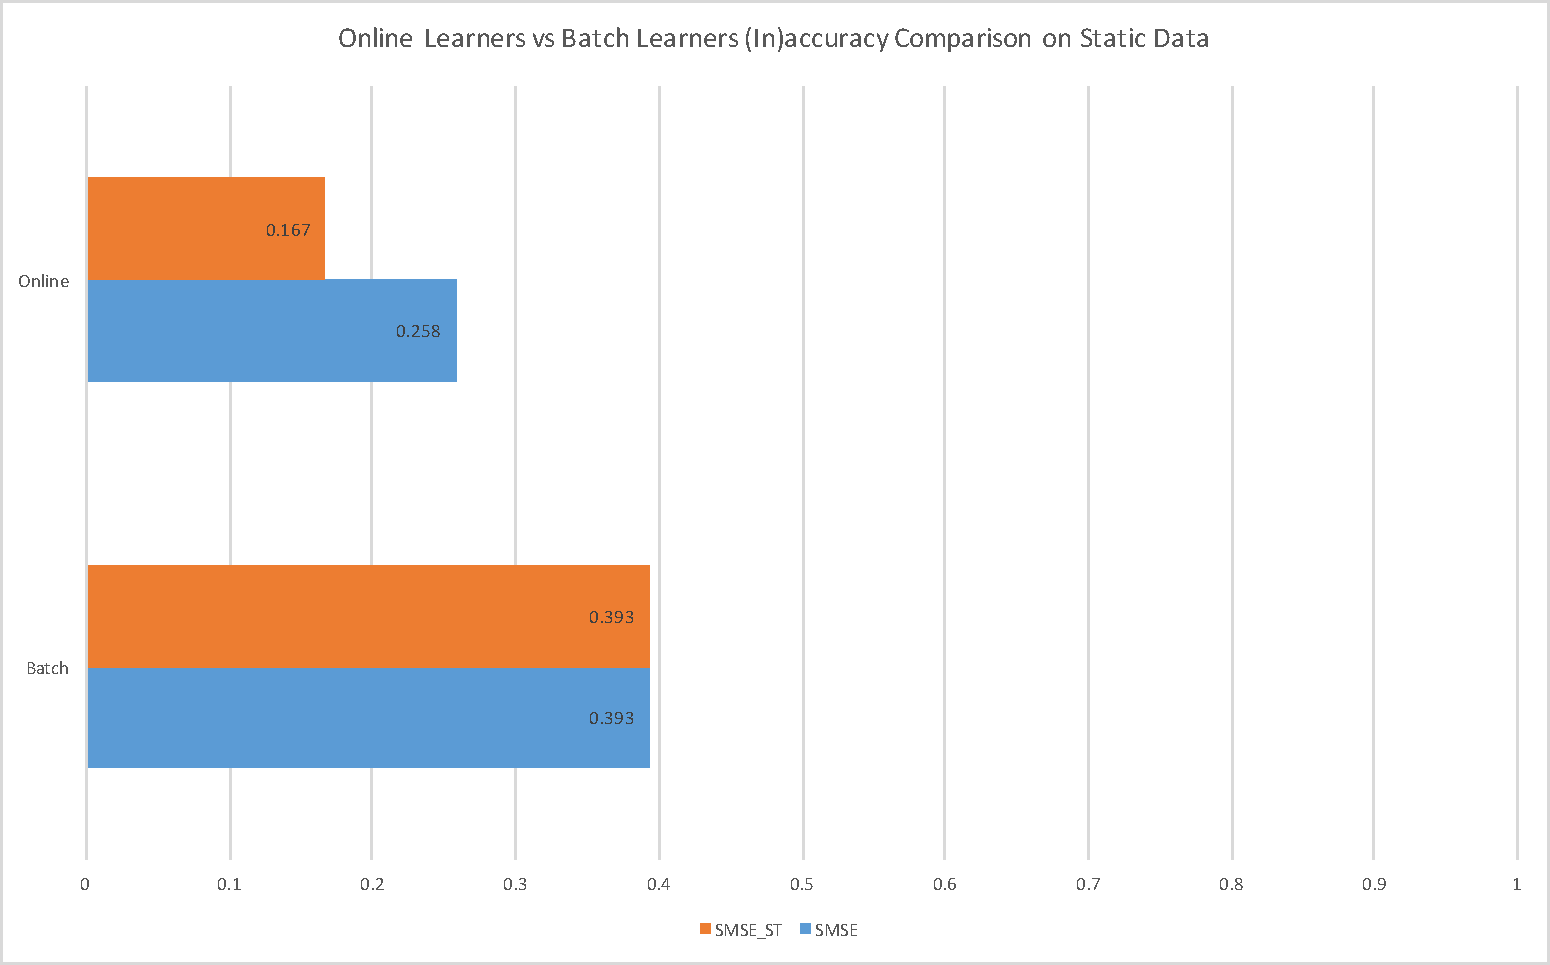
\includegraphics[width=\linewidth]{./Figures/batch_vs_online_inaccuracy_comp1.pdf}
  \caption{Inaccuracy Comparison of Batch and Online Learners. The bar values are obtained through aggregating the corresponding statistics over 576 stream simulations on 36 online learners and 576 tests on 12 batch learners respectively.}
  \label{fig:batch_vs_online_inaccuracy_comp1}
\end{figure}

In \ref{fig:batch_vs_online_inaccuracy_comp1}, what is shown is a \textit{rough} comparison of the accuracy of online learners and batch learners. It is a rough comparison because the first of two \texttt{SMSE} values shown are actually the average of already aggregated (over 576 streams) \texttt{SMSE} values of 52 online learners. As for the second value which is for the offline learners, it is similarly the average of already aggregated (over 576 synthetic data sets) \texttt{SMSE} values of 12 batch learners. According to this highly general results, the average accuracy difference of batch algorithms and online algorithms seems not to be very large in both \texttt{SMSE} and \texttt{SMSE\_ST} terms. Naturally, the average \texttt{SMSE} and \texttt{SMSE\_ST} values for Batch Learners are the same as they do not take any time to stabilize during the testing unlike their online counterparts. By looking at this results only, one might question the effort needed to design and implement online versions of batch learning algorithms since although the improvement is accuracy is still substantial with the online learners, batch ones did not have a worse \texttt{SMSE} than 0.4 which is acceptable. However, as said in the beginning, this rough results can be deceiving.

\begin{figure}[htbp]
  \centering
    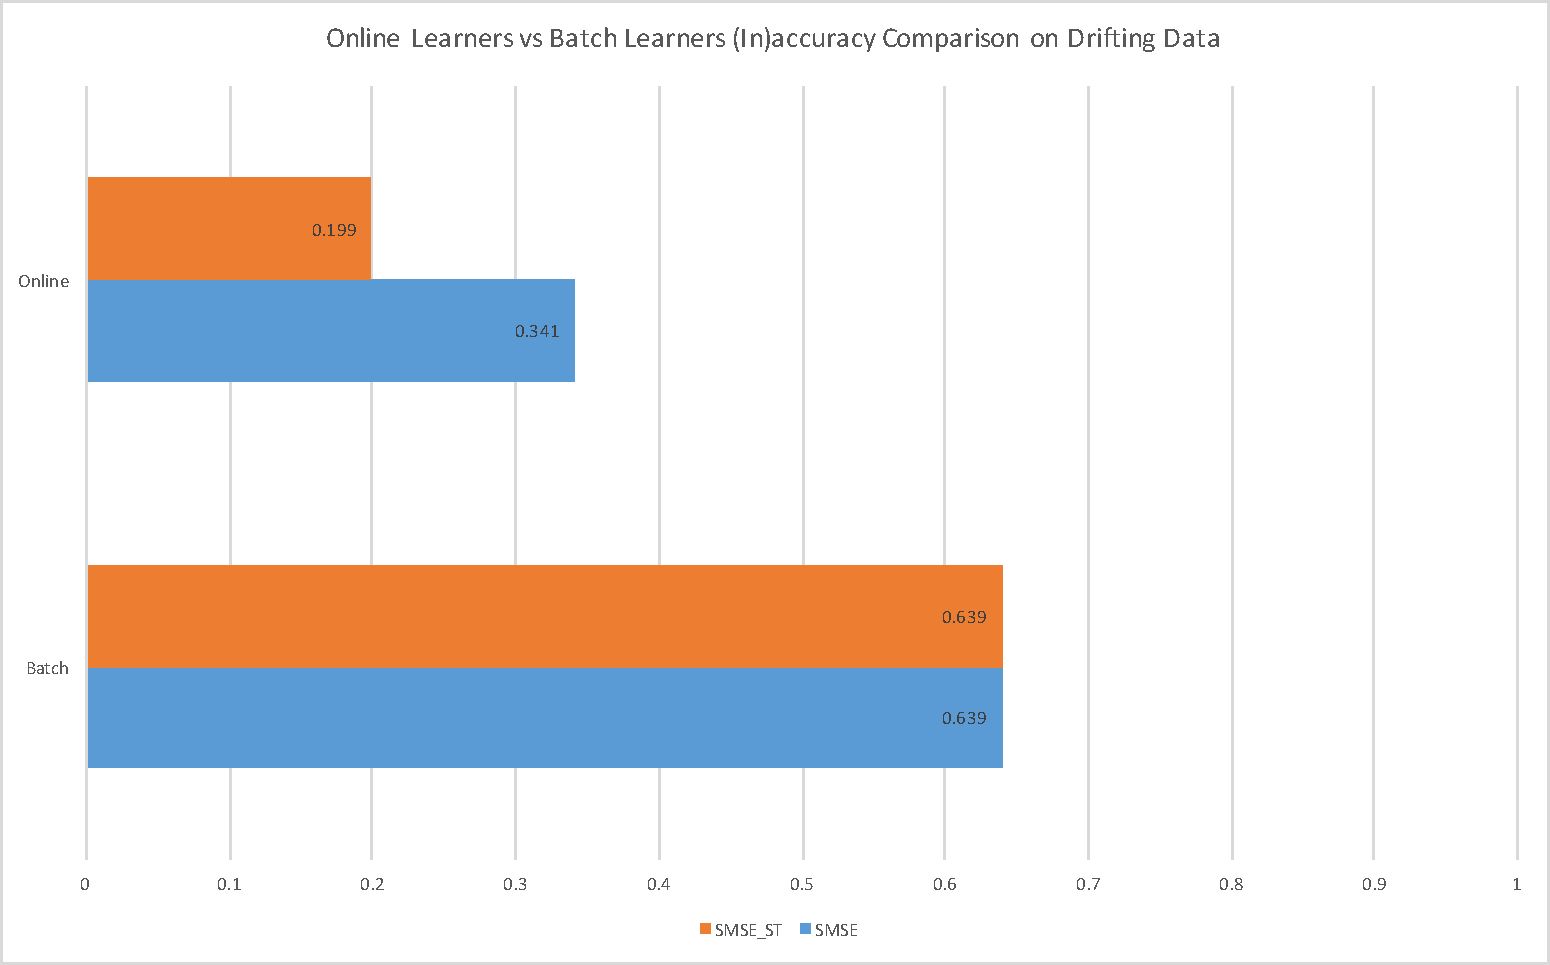
\includegraphics[width=\linewidth]{./Figures/batch_vs_online_inaccuracy_comp2.pdf}
  \caption{Inaccuracy Comparison of Batch and Online Learners on Non-Static Data. The bar values are obtained through aggregating the corresponding statistics over 276 stream simulations on 52 online learners and 276 tests on 12 batch learners respectively.}
  \label{fig:batch_vs_online_inaccuracy_comp2}
\end{figure}

If the accuracy results aggregated over tests with non-stationary data is analyzed, we see a totally different picture than \ref{fig:batch_vs_online_inaccuracy_comp1}. In \ref{fig:batch_vs_online_inaccuracy_comp2}, the accuracy gap between batch and online learners for non-static data tests is huge. What this means is if the changes in data distributions are expected during the online learning process, using a batch learner which is trained with test data beforehand is a very bad idea as the concept changes render the batch learners useless. One can reach this conclusion by looking at a side-by-side \texttt{RMSE} comparison of an individual batch learner and individual online learner on a single data stream \ref{fig:batch_vs_online_sidebyside_comp_res96}. In the simulated stream a concept change has affected the data points after the $1000_{th}$ stream item. We see that both algorithms perform equally well up until the concept drift. After the the drift occurs, the online algorithm was able to adapt itself to the change and recover its \textit{sliding window} error measured by the prequential method extension with sliding window of 128 while batch algorithm becomes \textit{useless}.

\begin{figure}[htbp]
  \centering
    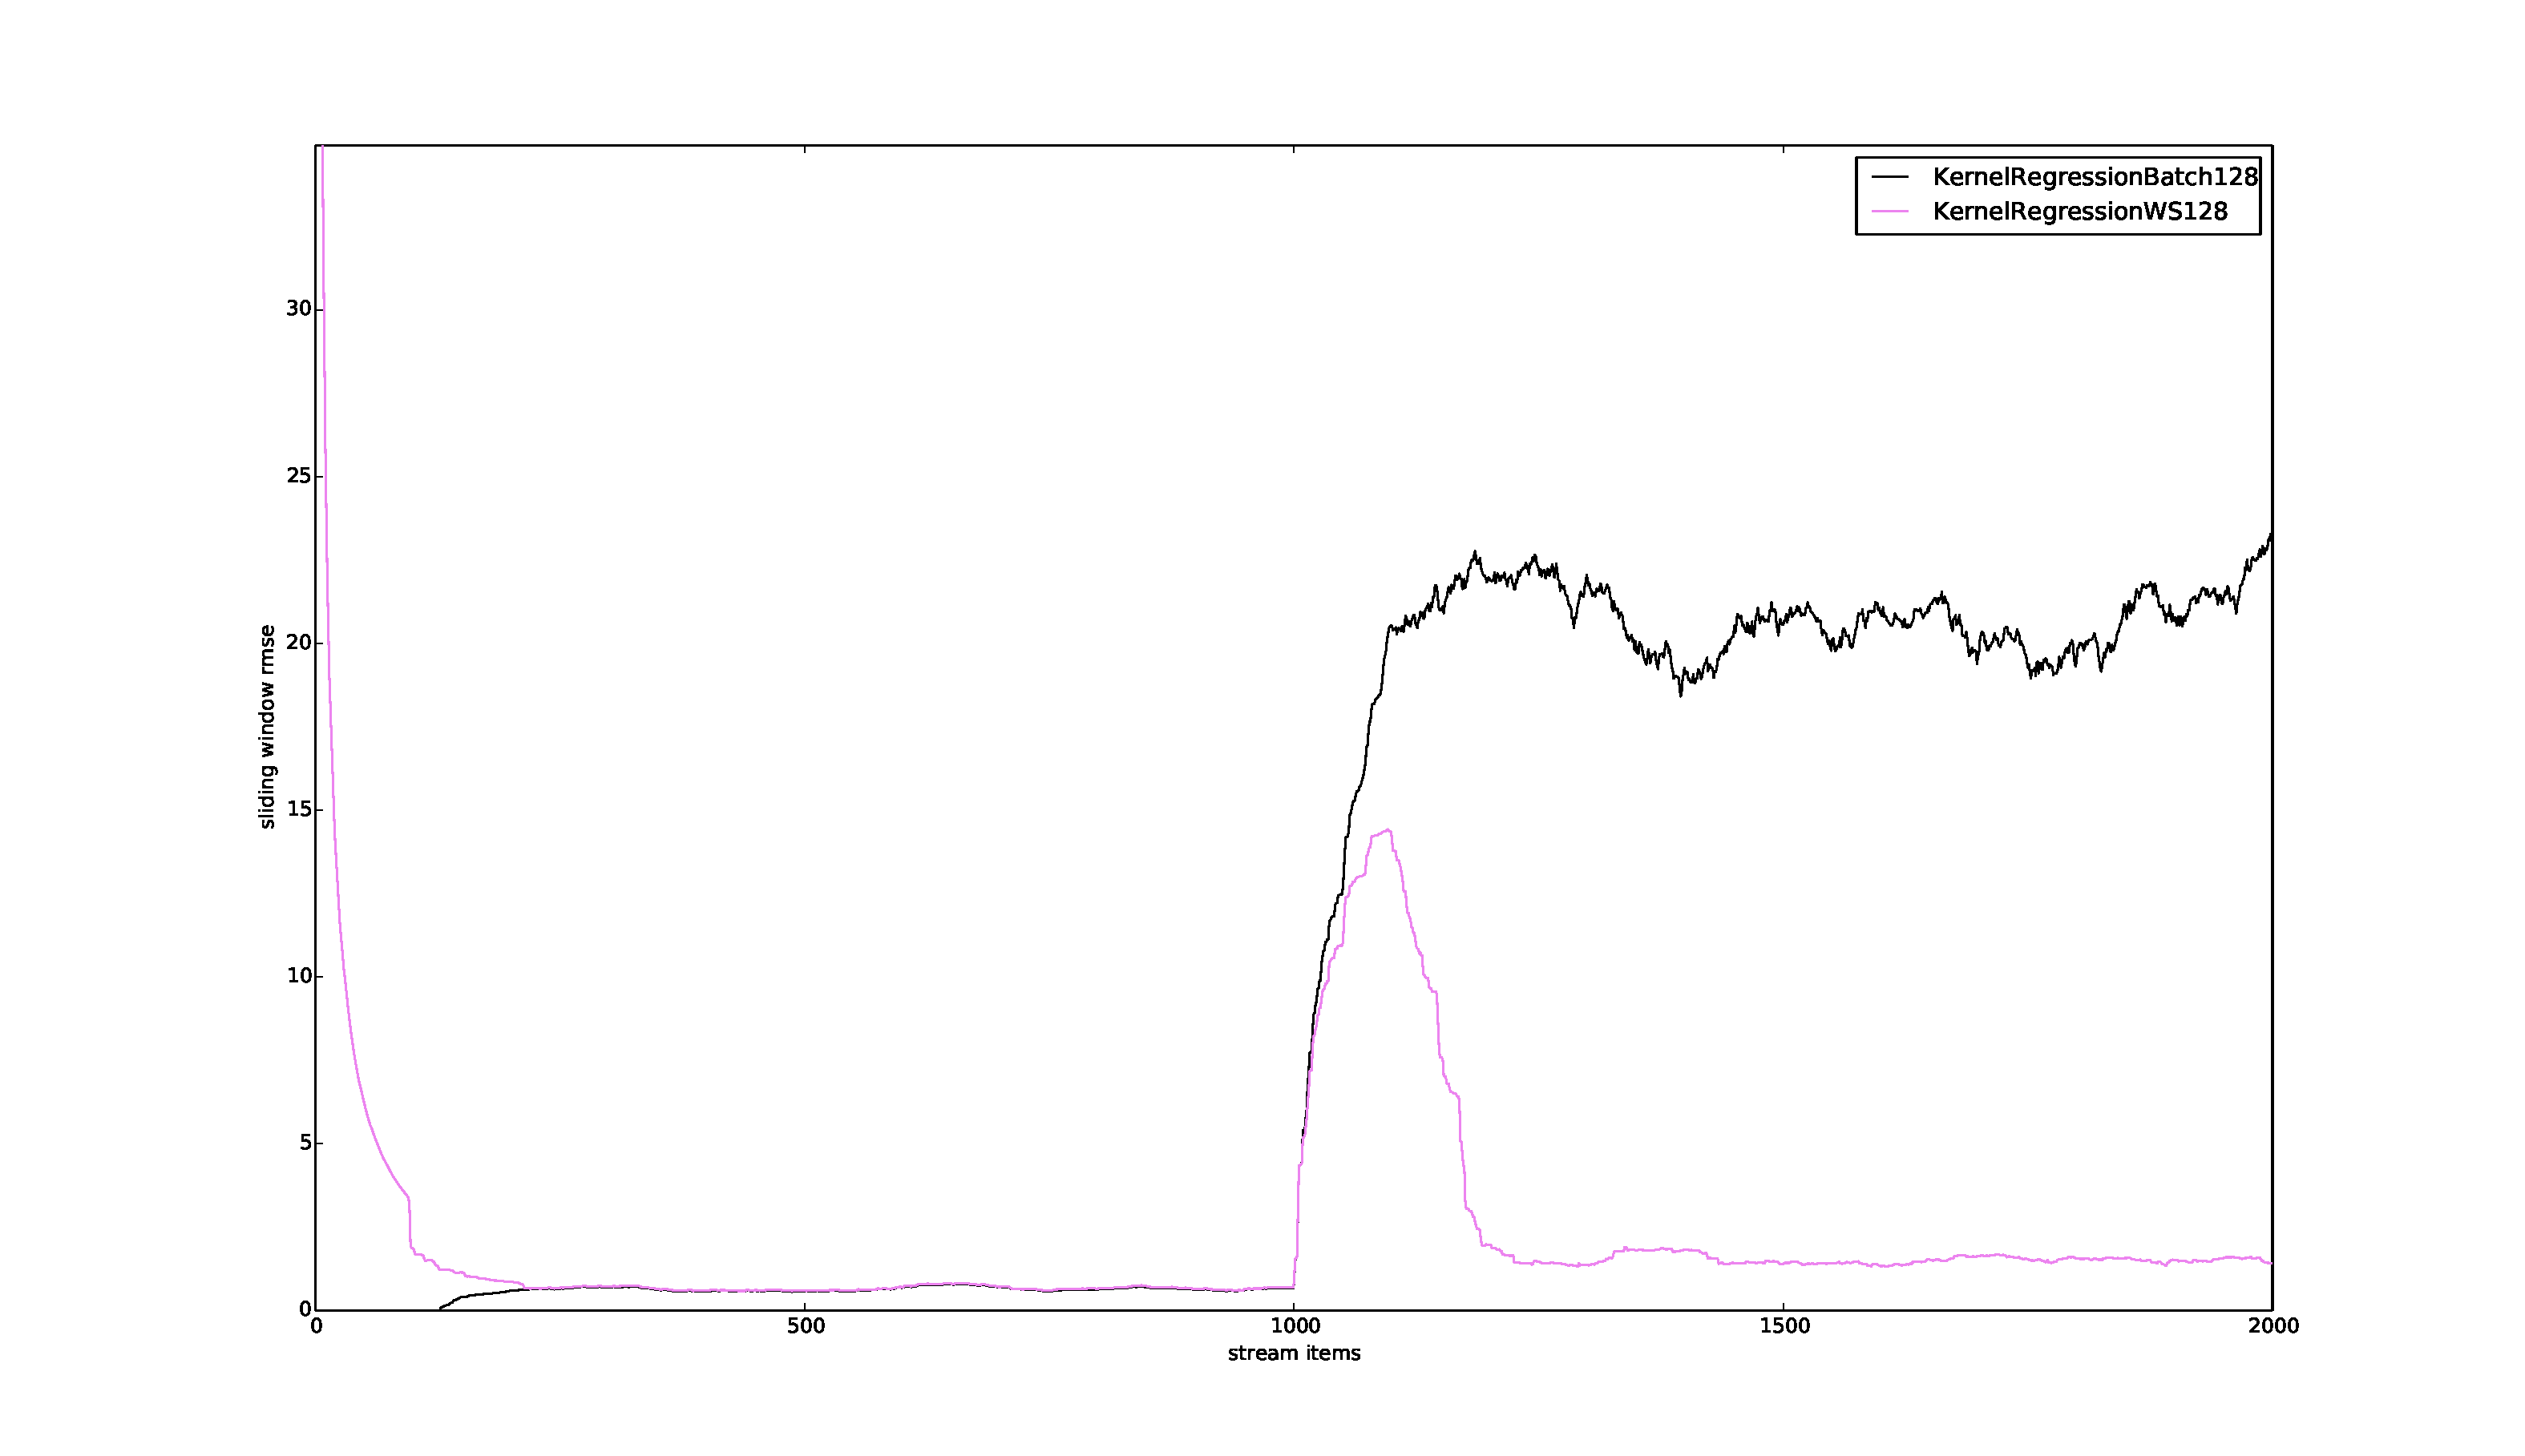
\includegraphics[width=\linewidth]{./Figures/batch_vs_online_sidebyside_comp_res96.pdf}
  \caption{Side-by-side Accuracy Comparison of Batch and Online versions of Kernel Regression with training set of 96 and sliding window size of 96 respectively. The test data used is SYNTH\_ND\_CD\_2000\_2\_10\_1\_22 and the resolution of the sliding error window accuracy evaluation method is set to 96}
  \label{fig:batch_vs_online_sidebyside_comp_res96}
\end{figure}

This first and the most fundamental observation validates the necessity of the use of online learning algorithms in streams. Rest of the analysis will rather concentrate on the comparison within the online learners.

\subsection{A general picture}

In \ref{fig:gen_alg_comparison}, we see the aggregated results of different family of online learning algorithms with 4 different metrics. The metrics used are the most critical ones in deciding which algorithm to deploy. Among the metrics used are \texttt{SMSE} that summarizes the accuracy, \texttt{SAIW} and \texttt{ICR} which together gives an overall opinion about the feasibility of the prediction bounds and lastly \texttt{ATPI} that allows to decide which algorithm category is quicker than the other in predicting the new data point. 

At first glance, it looks like the general accuracy scores (\texttt{SMSE}) of the algorithms are similar whereas in terms of static accuracy (\texttt{SMSE\_ST}), learners with parametric algorithms, \texttt{BayesianMLE} and \texttt{BayesianMAP}, are trailing behind of the non-parametric learners. All the families having the aggregate \texttt{SMSE} value lower than $0.28$ means that online learners were effective learning from streams in general so that all of them performed way better than the hypothetical trivial regression algorithm with \texttt{SMSE} of $1.0$ which returns the average of the targets observed until the point of prediction.

\begin{figure}[htbp]
  \centering
    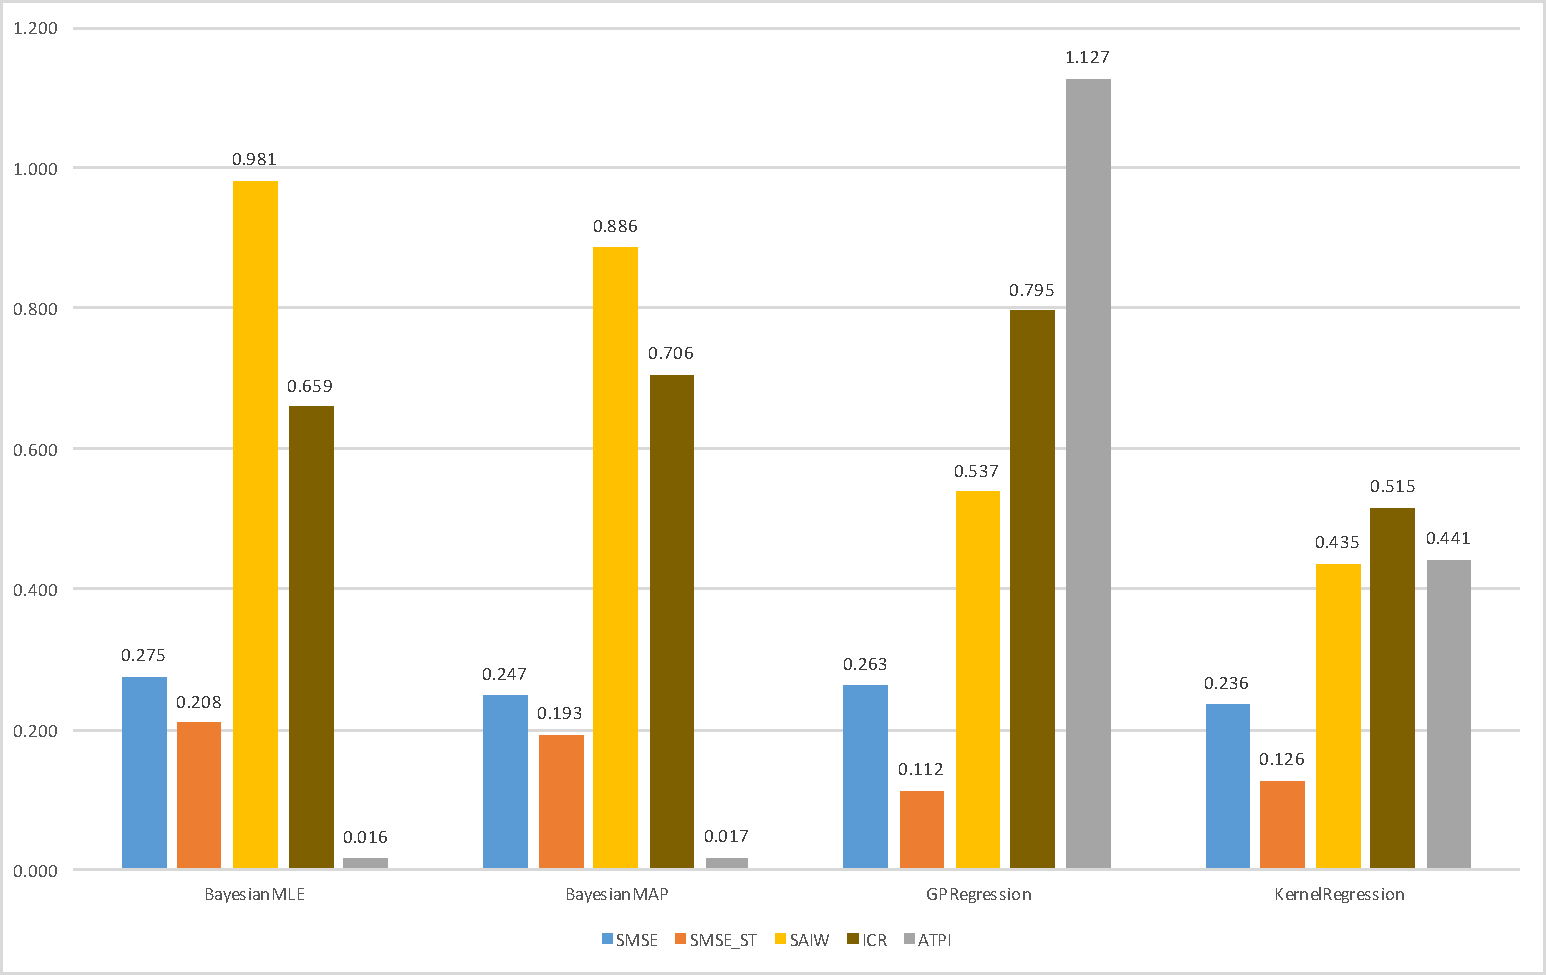
\includegraphics[width=\linewidth]{./Figures/gen_alg_comparison.pdf}
  \caption{A General Comparison of Online Algorithms. The values on columns are aggregated over 576 stream simulations on 52 online learners and grouped by the algorithm family.}
  \label{fig:gen_alg_comparison}
\end{figure}

As for a general comparison of prediction bounds quality, \texttt{KernelRegression} family provided the tightest prediction intervals for the predictions with the average \texttt{SAIW} score of $0.435$. However, in terms of the target coverage of its prediction bounds, it falls behind that of the algorithms of other families. This is not surprising as intuitively wider the prediction bounds are, higher the interval containment ratio is. This is also expected theoretically as discussed in Chapter \ref{Chapter3}, KernelRegression provides confidence intervals that are used as the prediction bounds rather than the prediction intervals which are known to be wider. This graph alone does not say anything conclusive on the quality of prediction bounds that \texttt{KernelRegression} Family provides. Both \texttt{BayesianMLE} and \texttt{BayesianMAP} families have very high \texttt{SAIW} scores (between $0.85$ and $1.0$) meaning that their prediction bounds are almost as big as the overall scale of the target variable. For a single algorithm variant, this alone would be enough to conclude that it is unsuitable for a an application where the online learner to be deployed to does not have a tolerance for wide prediction bounds. However, in the graph, results are aggregated over different variants within the individual algorithm families presented. That is why, it is hard to conclude anything from it. Moreover, \texttt{GPRegression} family has the best \texttt{ICR} score and counterintuitively its \texttt{SAIW} score, $0.535$, is not very high. This indicates that, generally speaking, in terms of prediction bounds, \texttt{GPRegression} family is able to produce good prediction intervals.

In terms of average prediction time which is a very crucial consideration in stream learning scenarios, parametric families, \texttt{BayesianMLE} and \texttt{BayesianMAP}, proved to be very quick with the average ATPI score on the ballpark of 15 $\mu s$. Non-parametric models are relatively slower. \texttt{KernelRegression} family could process stream items with 441 $\mu s$ latency on average, Not so surprisingly due to its sophisticated prediction and update mechanism involving heavy matrix operations together with costly tuning routine that involves a non-convex optimization task, \texttt{GPRegression} family is the slowest with the average item processing latency of 1127 $\mu s$.

As pointed out, it is not possible to draw any significant and concrete conclusions from this general analysis. This is why, it is necessary to further examine the test data by drilling down to more details. To this end, the following sections include a more detailed analysis on the behavior of learners with changing qualities of either themselves (e.g window size, forgetting factor) or of the learning environment (e.g input dimensionality, noise variance, target scale).

\subsection{Sliding window size}

In \ref{fig:ws_on_accuracy1}, on the x- axis we see five different window sizes used in online learners featuring sliding window mechanism. \texttt{SMSE\_ST} values improve (decreases) as the window size gets bigger expectedly. This must be due to the bigger \textit{case base} upon which the predictions of the online algorithm are based. A similar situation exists in batch algorithms with the changing training set size. As shown in \ref{fig:batch_trainingsetsize_on_accuracy}. This is a simple implication of sliding window semantically being a \textit{dynamically} evolving training set. However, this relation between the sliding window size and the accuracy seem to hold only in the case of \texttt{SMSE\_ST} statistic which excludes the prediction errors that online learners make during the \textit{adaptation} periods either before its sliding window gets full or after an abrupt concept drift. 

\begin{figure}[htbp]
  \centering
    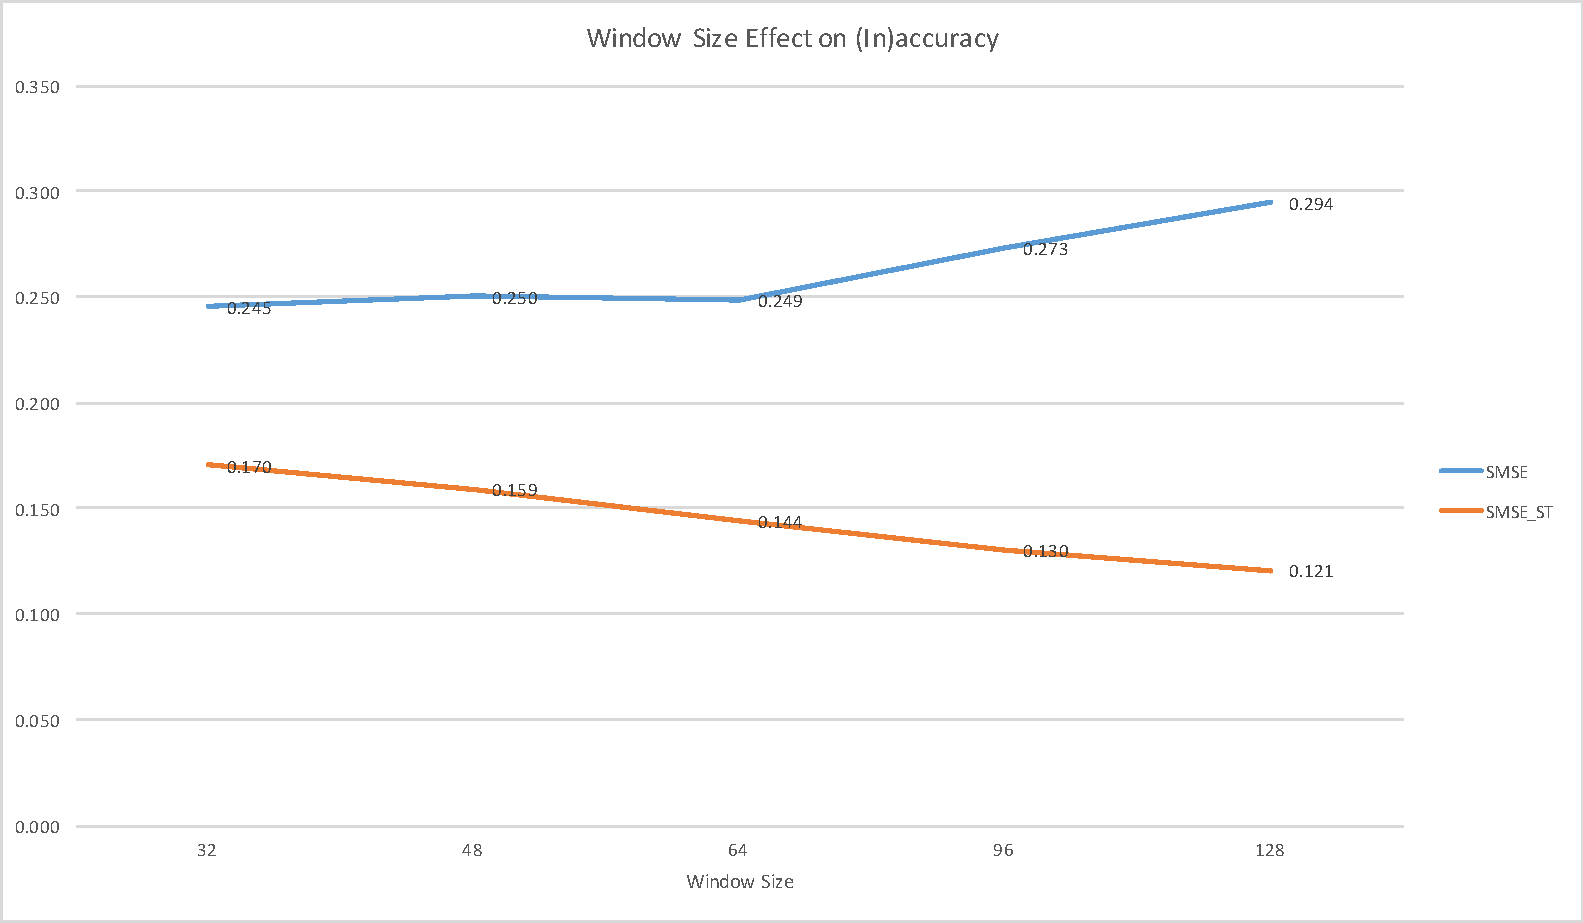
\includegraphics[width=\linewidth]{./Figures/ws_on_accuracy1.pdf}
  \caption{Accuracy comparison of sliding windowed learners with varying window sizes. \texttt{SMSE} and \texttt{SMSE\_ST} values are aggregated over 576 stream simulations on 8 sliding windowed online learners (2 BayesianMAP, 2 BayesianMLE, 3 GPRegression and 1 KernelRegression variants) for each window size}
  \label{fig:ws_on_accuracy1}
\end{figure}

\begin{figure}[htbp]
  \centering
    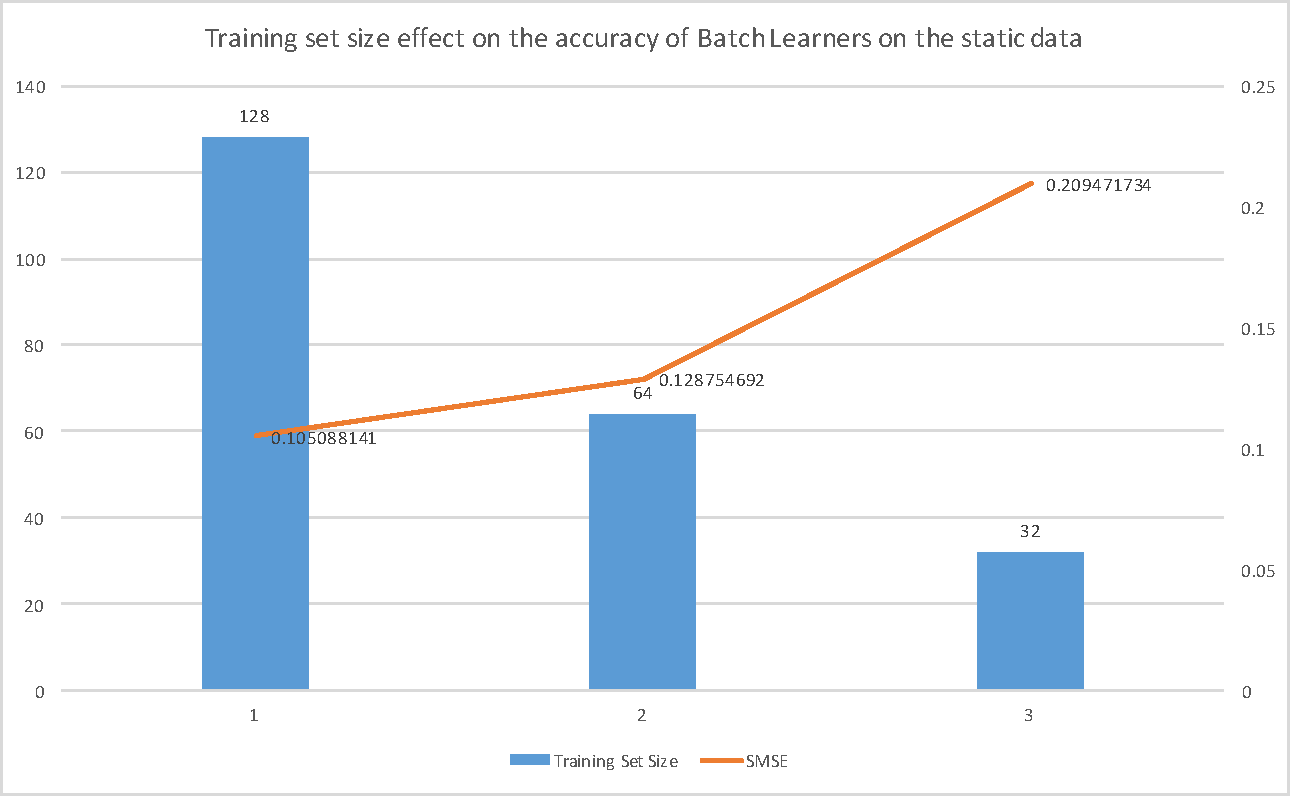
\includegraphics[width=\linewidth]{./Figures/batch_trainingsetsize_on_accuracy.pdf}
  \caption{Accuracy comparison of batch learners with varying training set sizes. \texttt{SMSE} values are aggregated over 288 tests (with static data) on 4 different batch algorithm for each training set size}
  \label{fig:batch_trainingsetsize_on_accuracy}
\end{figure}

If we examine the change in \texttt{SMSE} values with changing window size, something which cannot be explained trivially is observed: The highest choice of the sliding window size, being $128$, resulted in the poorest \texttt{SMSE} result in the averaged test results. Knowing the difference between the computed statistics \texttt{SMSE} and \texttt{SMSE\_ST}, one could link this phenomenon of accuracy drop as the window size increases to the relatively higher stabilization time learners with bigger sliding windows need after concept drifts. In order to validate this claim, one needs to analyze the evolution of the accuracy as a function of time. As discussed previously, the proposed extensions to the prequential evaluation method extensions provide such time-dependent analysis. However, this time the analysis will be confined to an individual test case (single stream simulation) as these extensions forbid the aggregations over different tests. 

\begin{figure}[htbp]
  \centering
    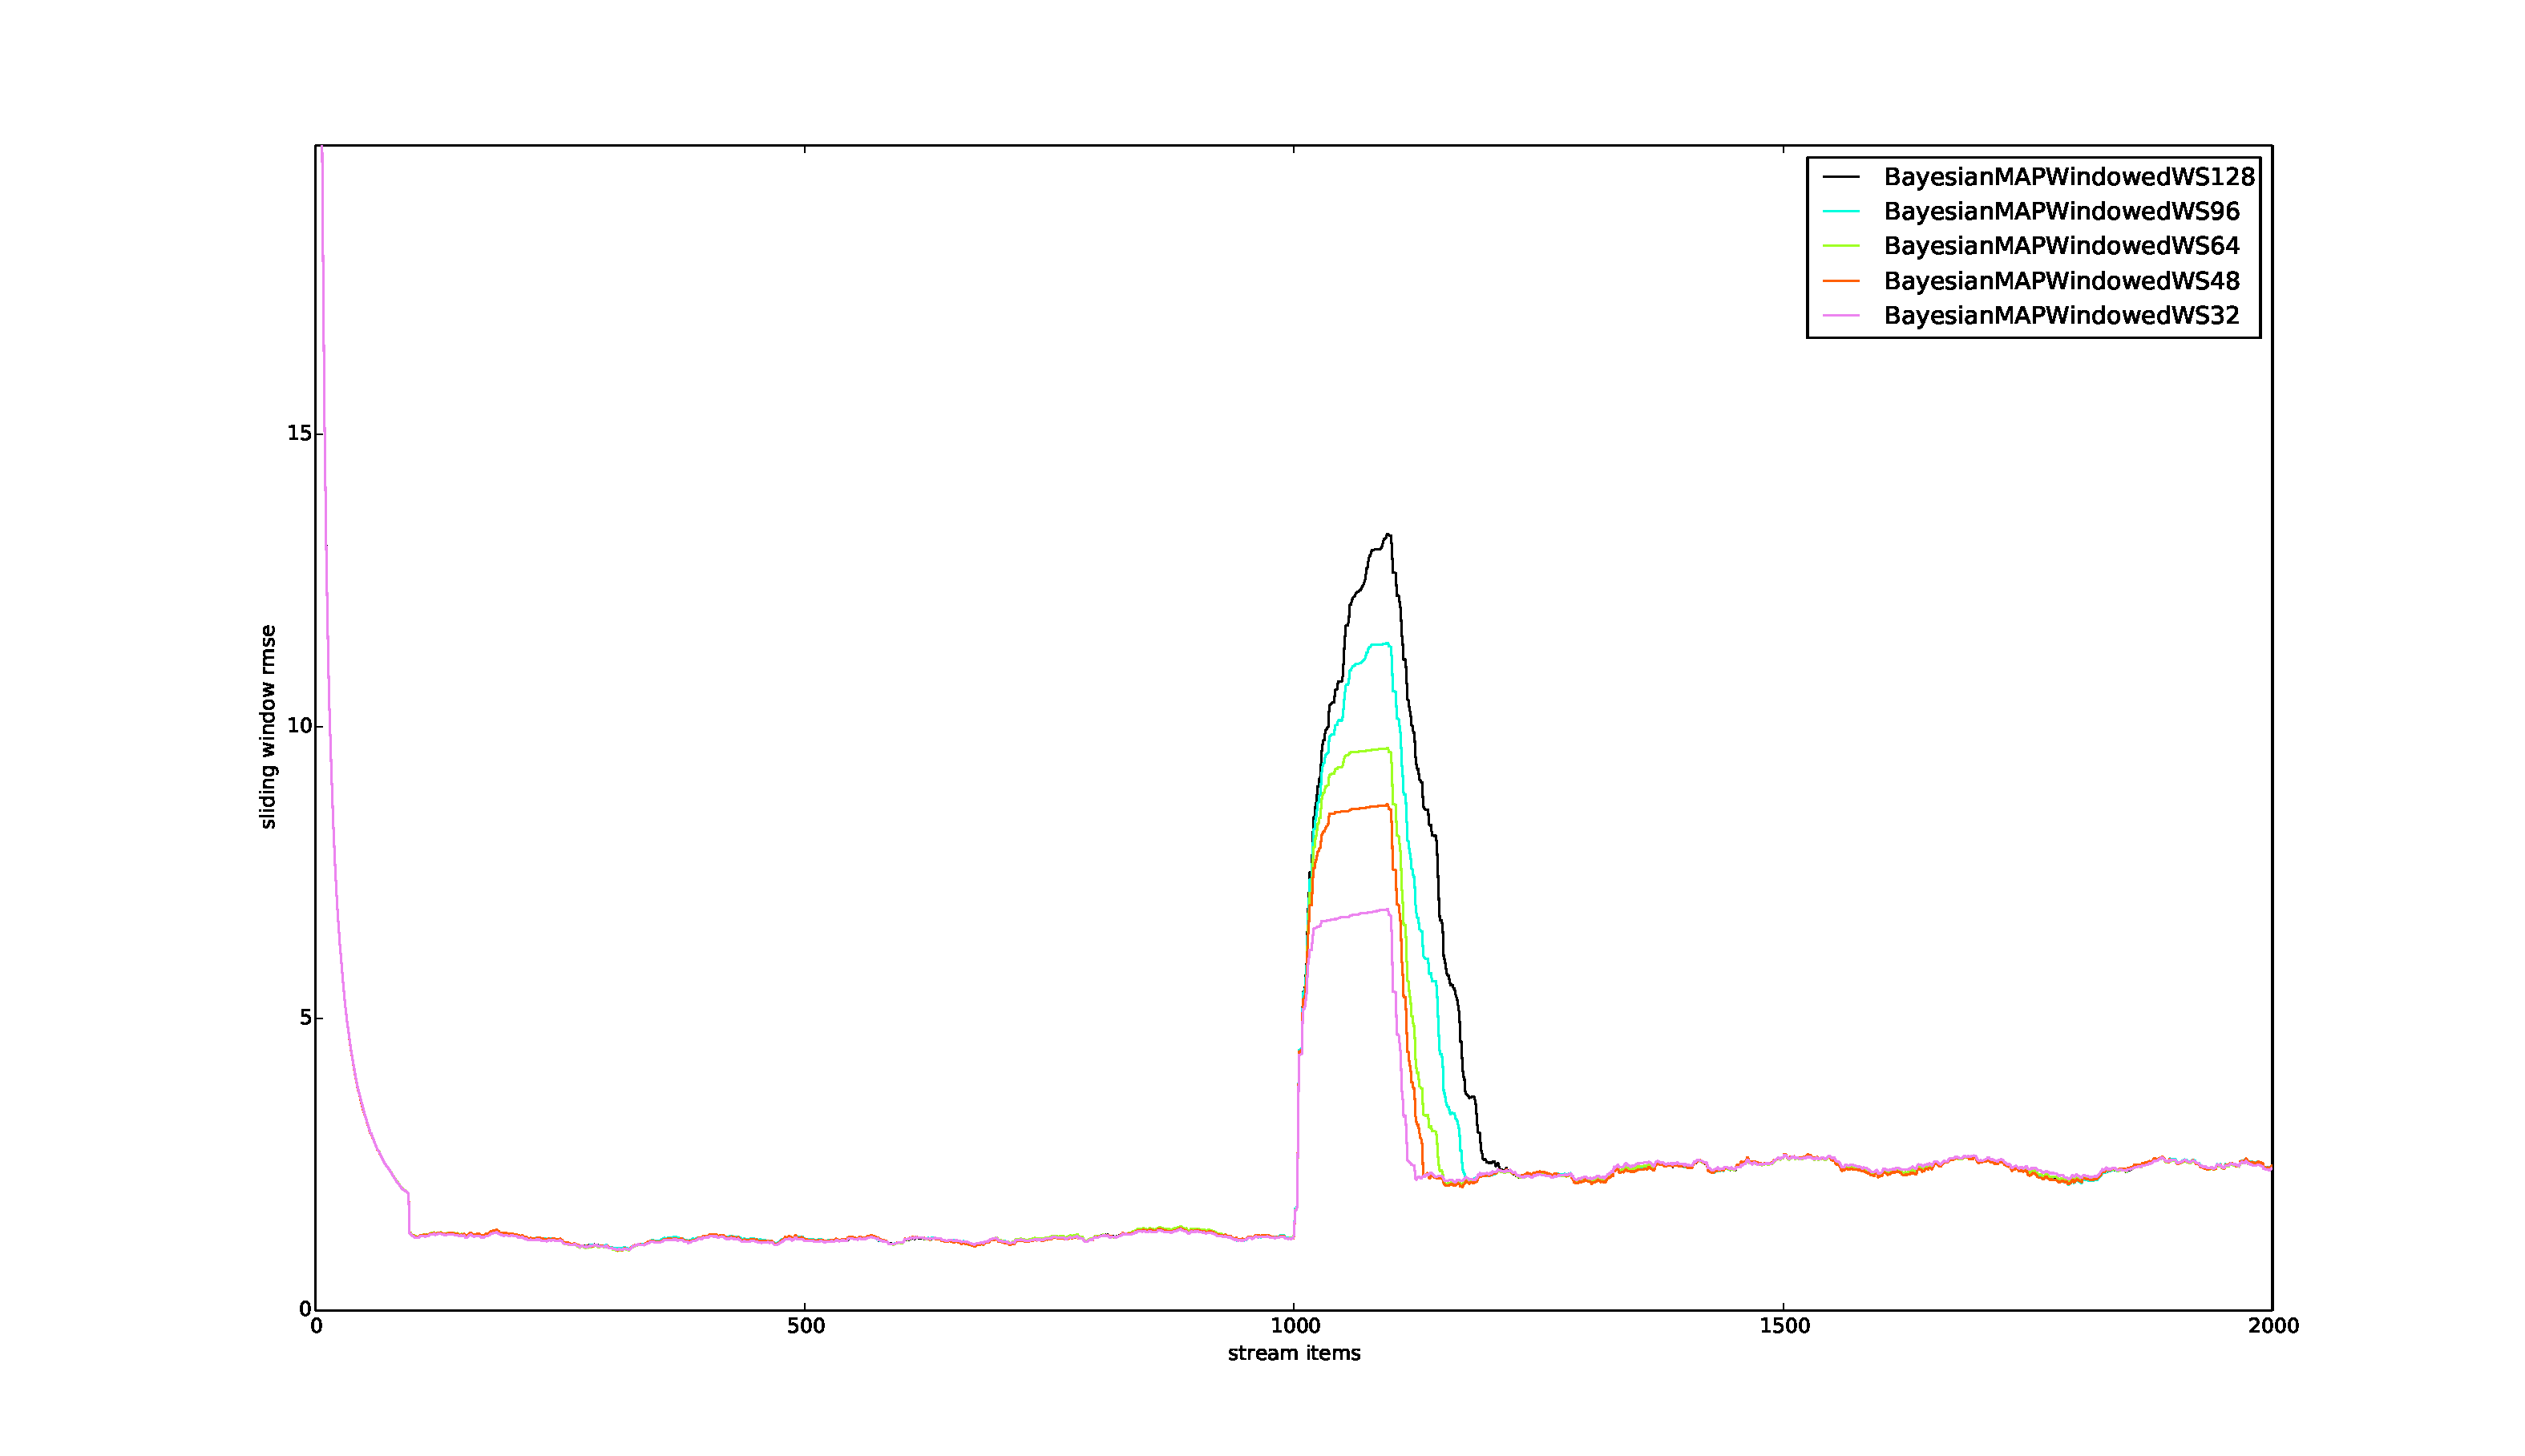
\includegraphics[width=\linewidth]{./Figures/wsize_on_stabilization_sidebyside_comp_res96.pdf}
  \caption{Side-by-side Accuracy Comparison of \texttt{BayesianMAPWindowed} with different window sizes. The test data used is \texttt{SYNTH\_ND\_CD\_2000\_2\_10\_1\_22} and the resolution of the sliding error window accuracy evaluation method is set to 96}
  \label{fig:wsize_on_stabilization_sidebyside_comp_res96}
\end{figure}

\begin{figure}[htbp]
  \centering
    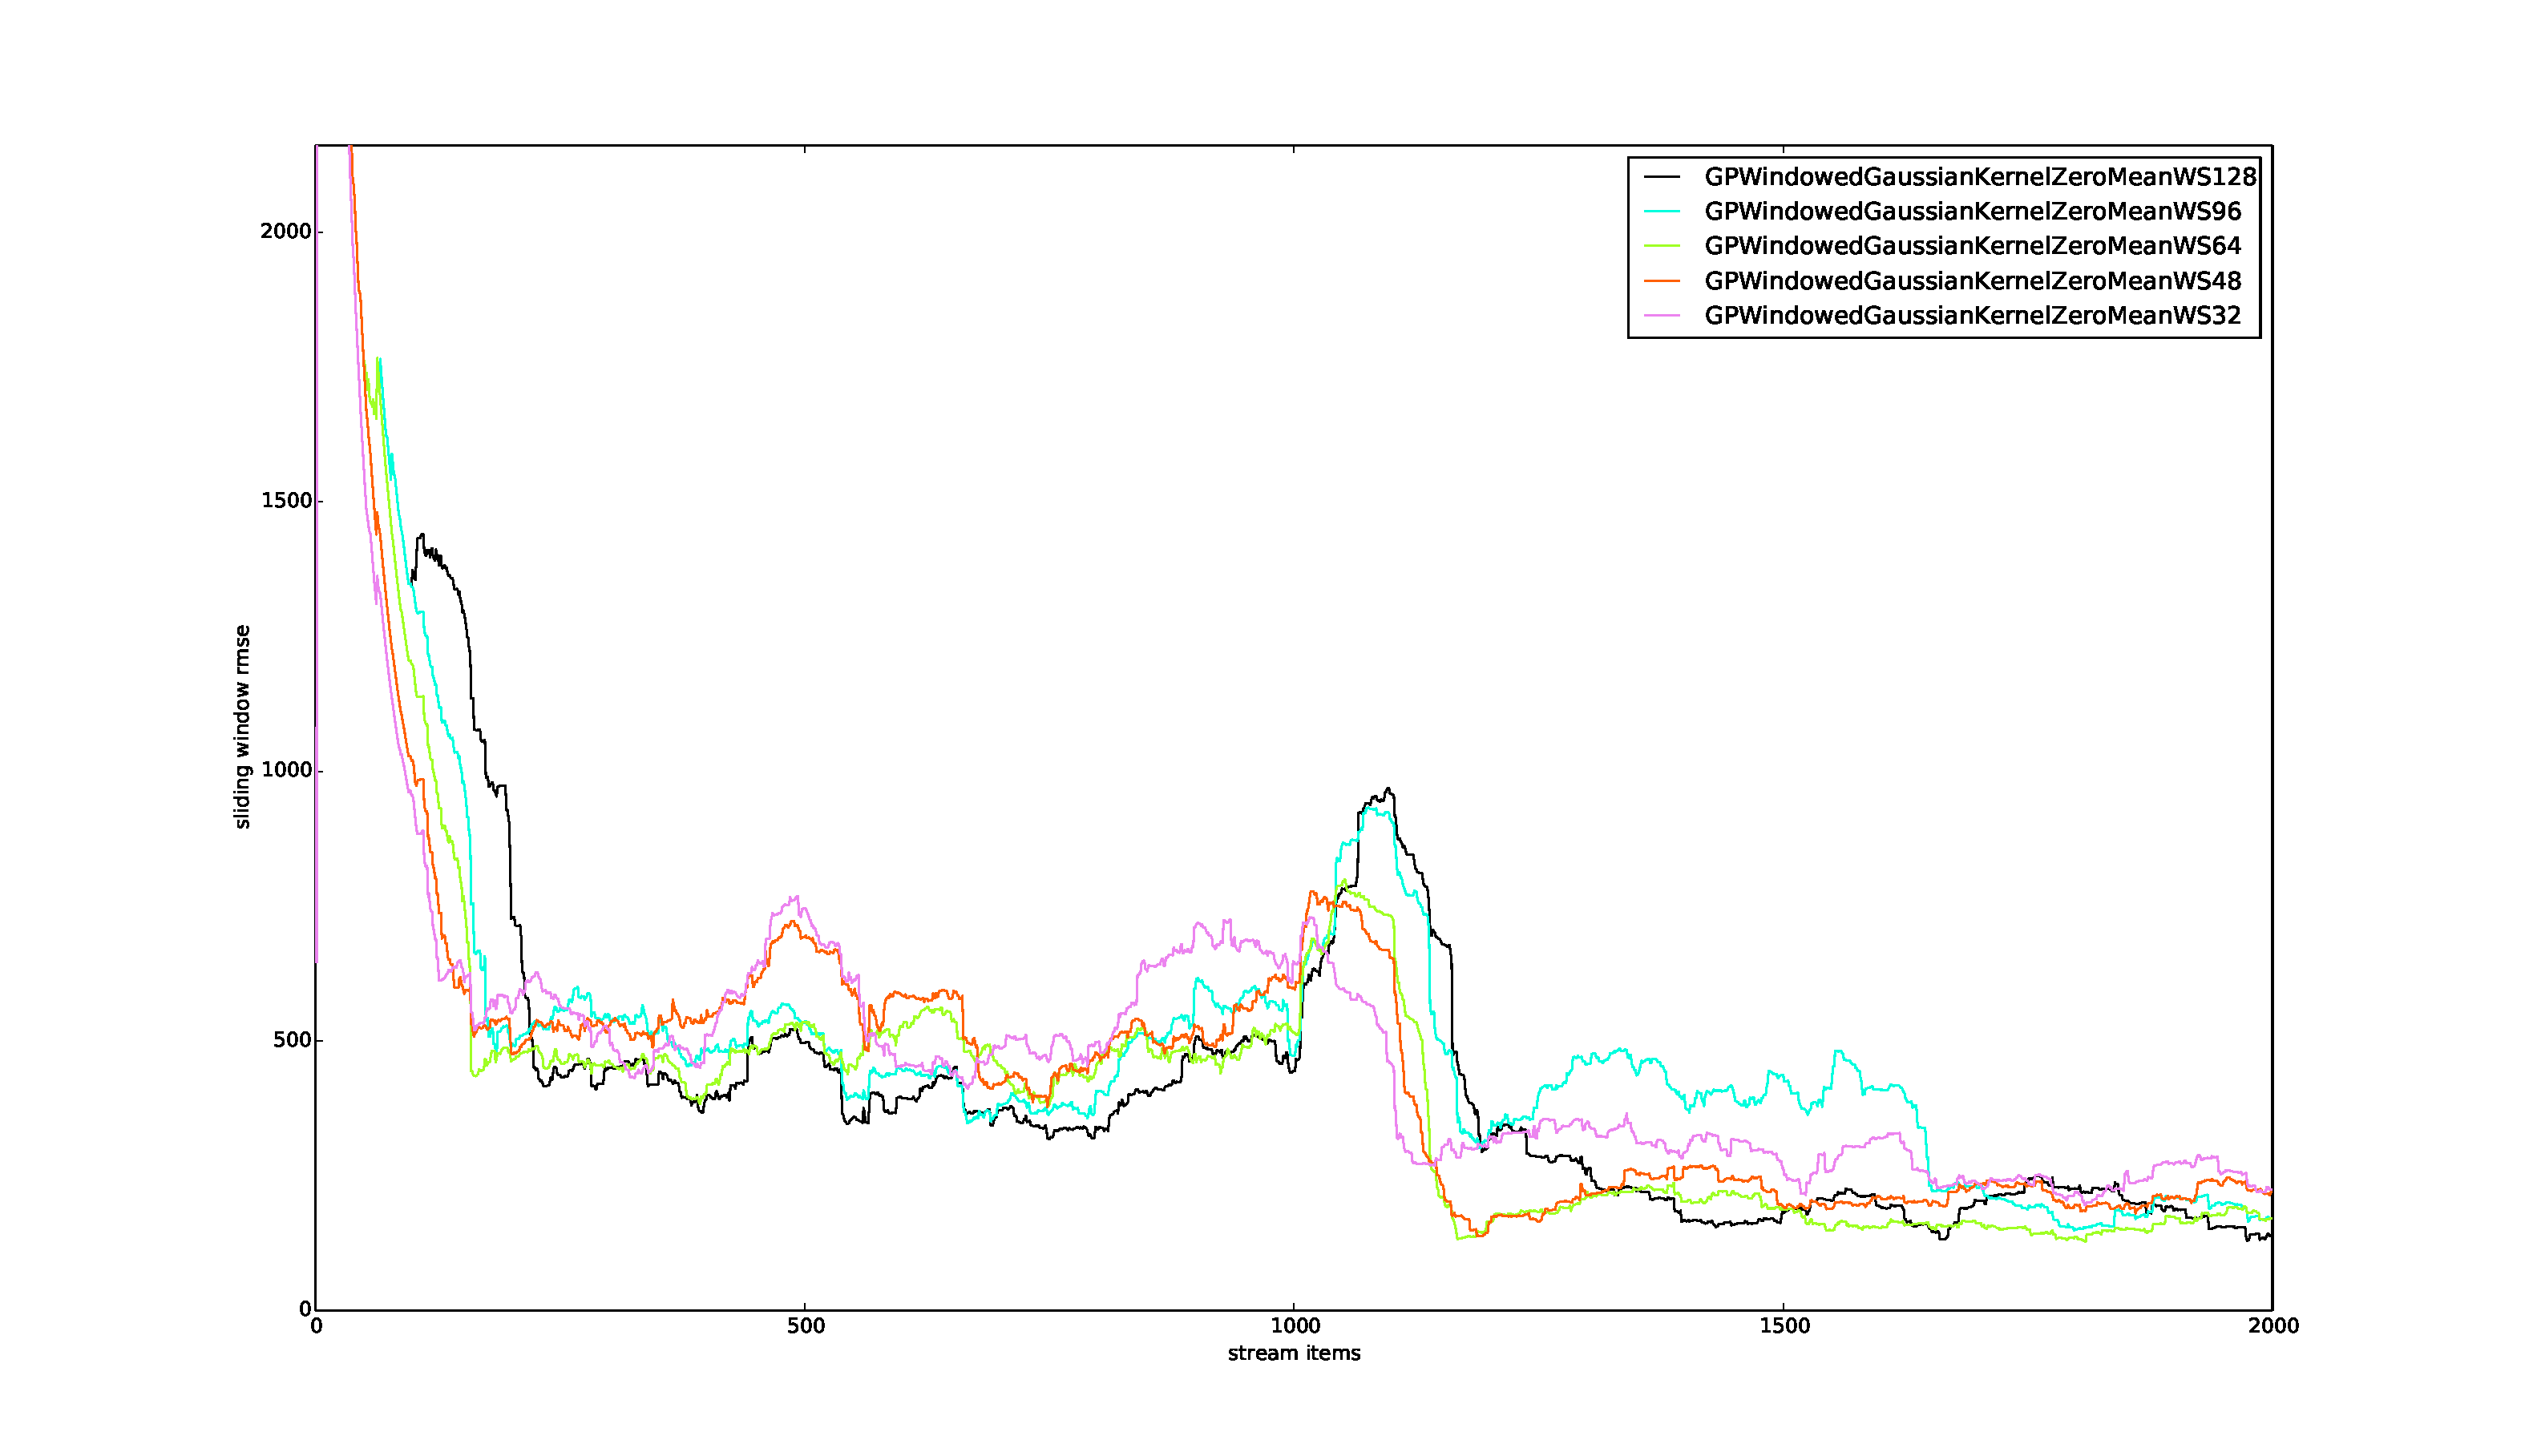
\includegraphics[width=\linewidth]{./Figures/wsize_on_stabilization2_sidebyside_comp_res96.pdf}
  \caption{Side-by-side Accuracy Comparison of Online \texttt{GPWindowedGaussianKernelZeroMean} variants with different window sizes. The test data used is \texttt{SYNTH\_D\_CD\_2000\_4\_10\_1\_24} and the resolution of the sliding error window accuracy evaluation method is set to 96}
 \label{fig:wsize_on_stabilization2_sidebyside_comp_res96}
\end{figure}

In \ref{fig:wsize_on_stabilization_sidebyside_comp_res96} and \ref{fig:wsize_on_stabilization2_sidebyside_comp_res96}, it is clearly seen that after the concept drift the learner with the biggest window size took the longest time to adapt to the changing data distribution. This is not surprising because the sliding window algorithms implemented incorporate the new items one by one after their update mechanism is triggered by high error and until the \textit{deceiving} the data points left in the window from the previous concept are replaced with the new ones, the predictions will suffer from big errors as what is \textit{assumed} to be the reference data points (case base) in building the predictive model internally by the learner are far off in the mentioned unstable phase. This may or may not result in poor general accuracy scores (\texttt{SMSE}) depending on the how big the increased accumulated error term is during the unstable learning periods and the overall accuracy improvement in the stable learning periods with the higher window size. In the experiments carried out, it is observed that the average \texttt{SMSE} result remained the same when the window size is increased from $48$ to $64$ possibly because of the increased stable accuracy compensating the longer unstable period producing larger number of erroneous predictions resulting in unchanged general accuracy. The explained relations between the stable and total accuracy with the window size are inherently present in the case of any sliding-window algorithm regardless of the algorithm used to build a predictive model from the data points stored in the sliding window. 

\begin{figure}[htbp]
  \centering
    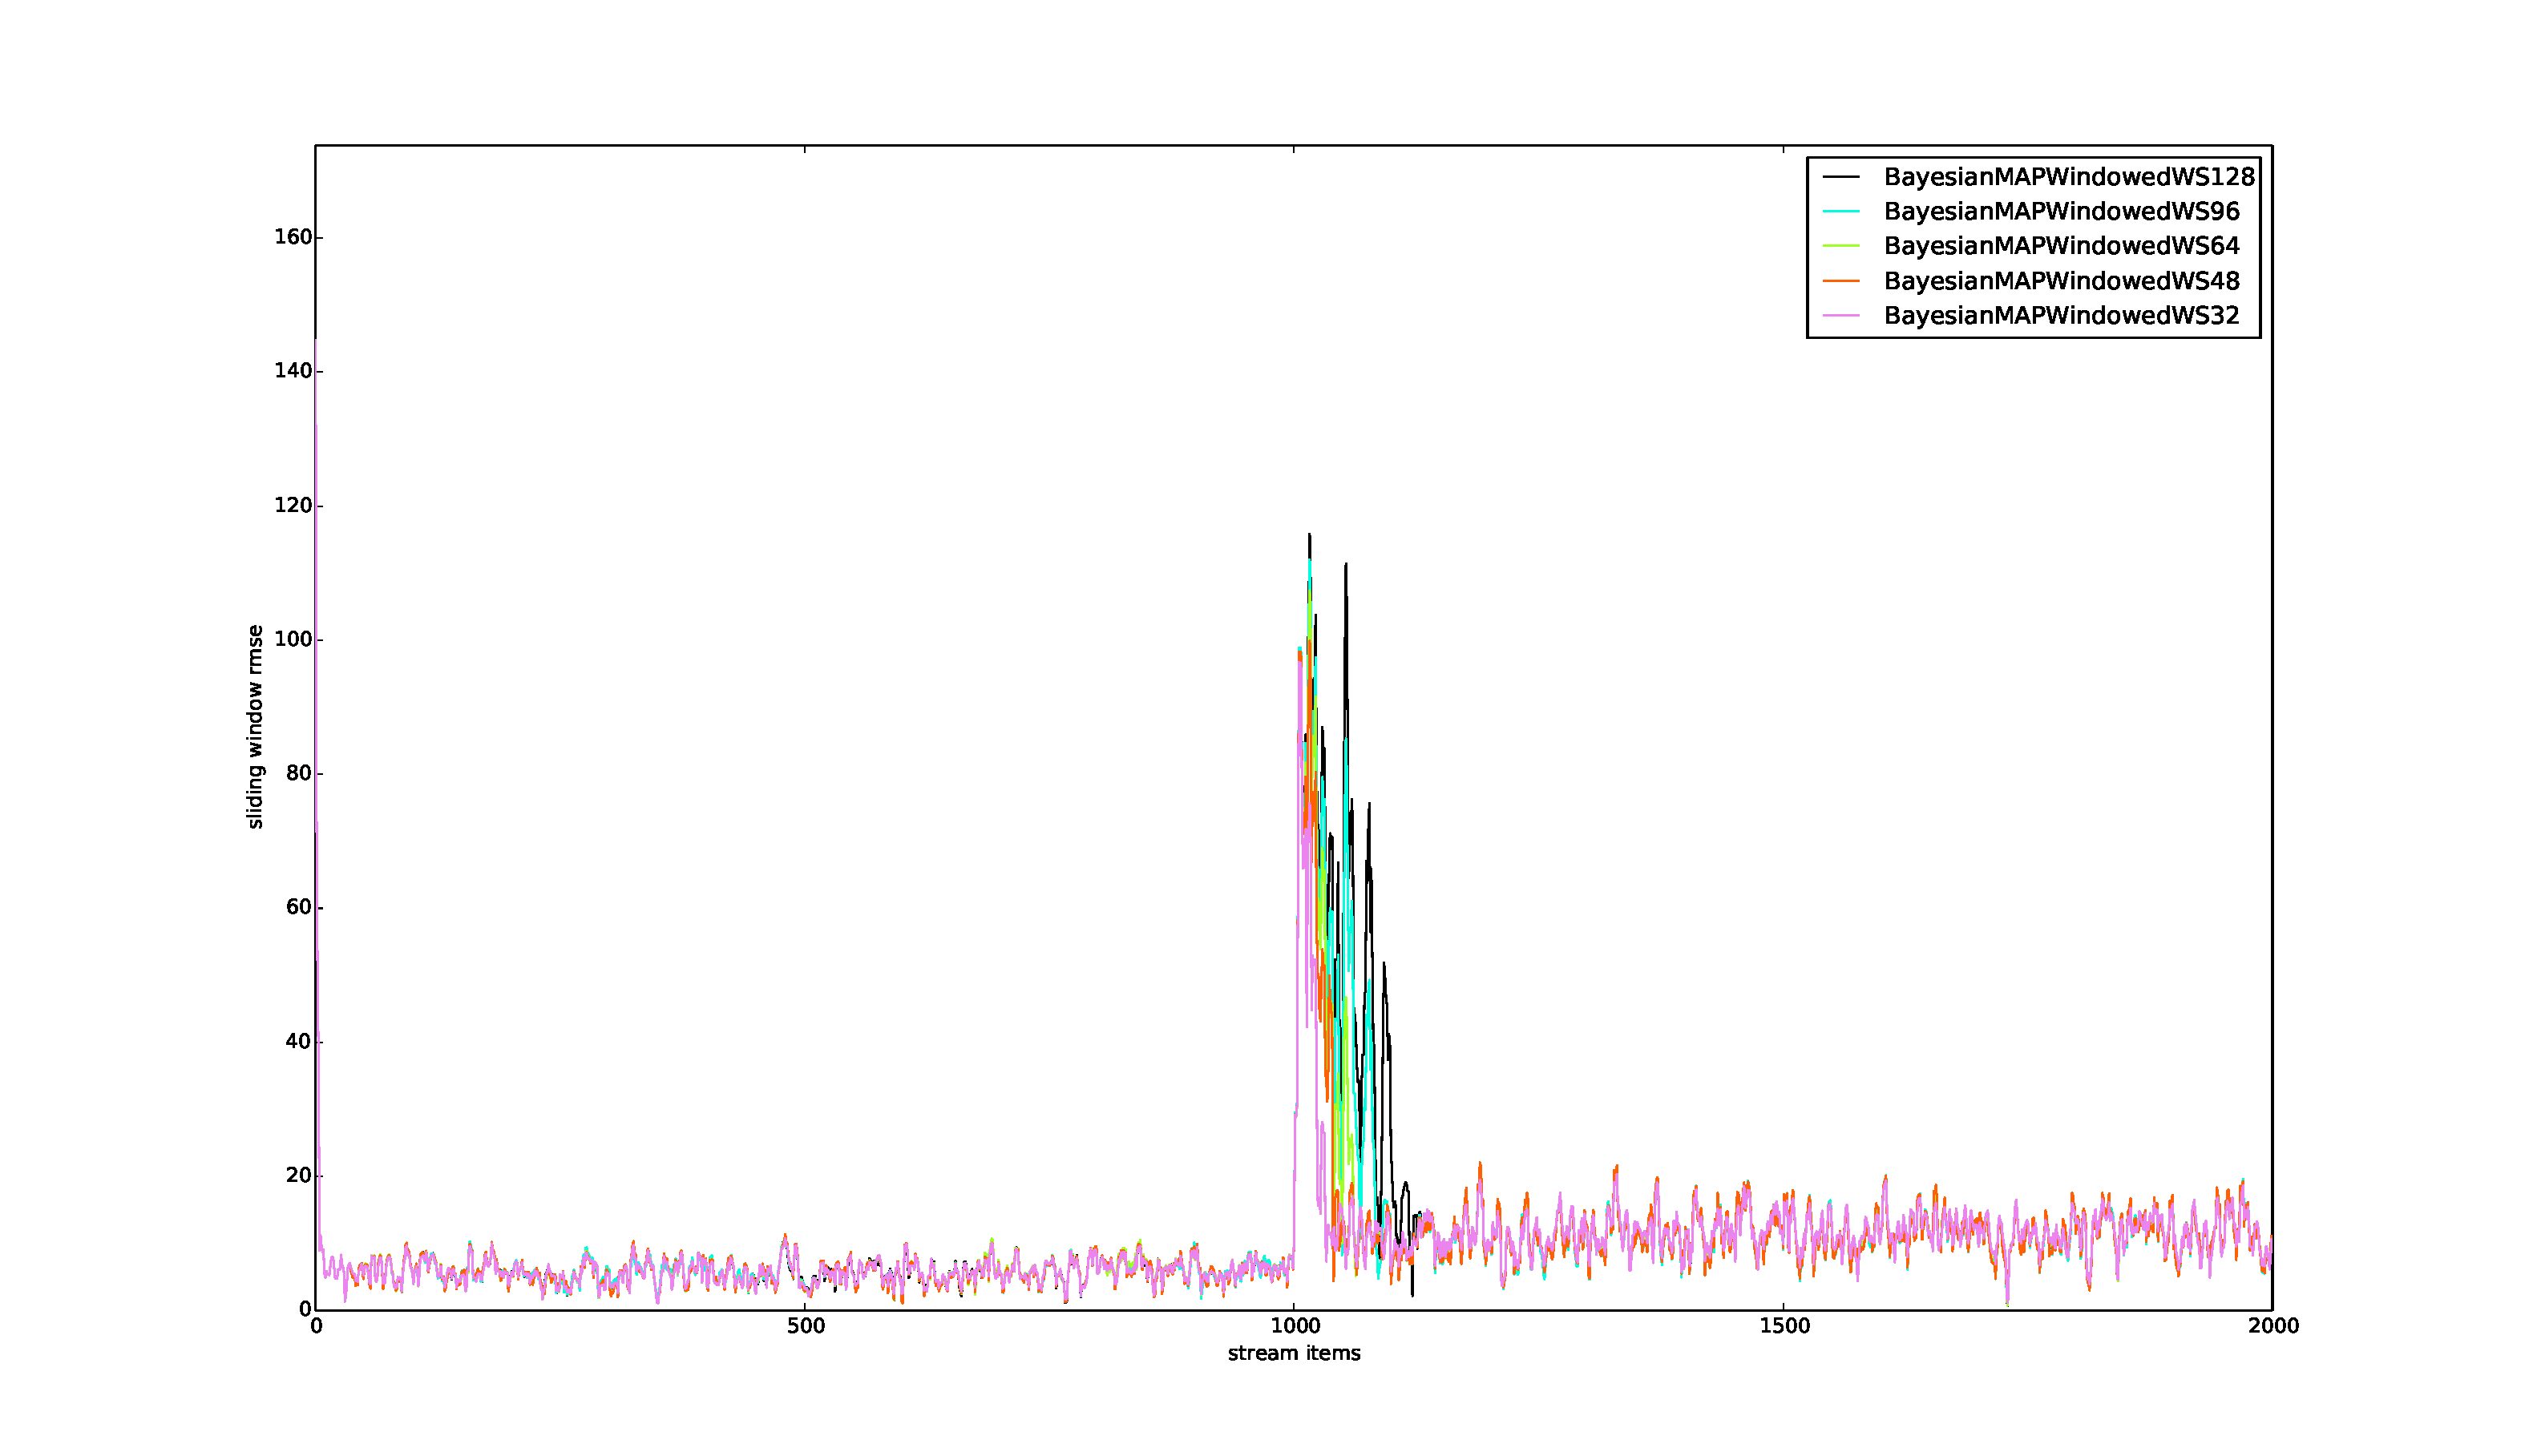
\includegraphics[width=\linewidth]{./Figures/wsize_on_stabilization_sidebyside_comp_res4.pdf}
  \caption{Side-by-side Accuracy Comparison of \texttt{BayesianMAPWindowed} variants with different window sizes. The test data used is \texttt{SYNTH\_ND\_CD\_2000\_2\_10\_1\_22} and the resolution of the sliding error window accuracy evaluation method is set to 4}
  \label{fig:wsize_on_stabilization_sidebyside_comp_res4}
\end{figure}

\begin{figure}[htbp]
  \centering
    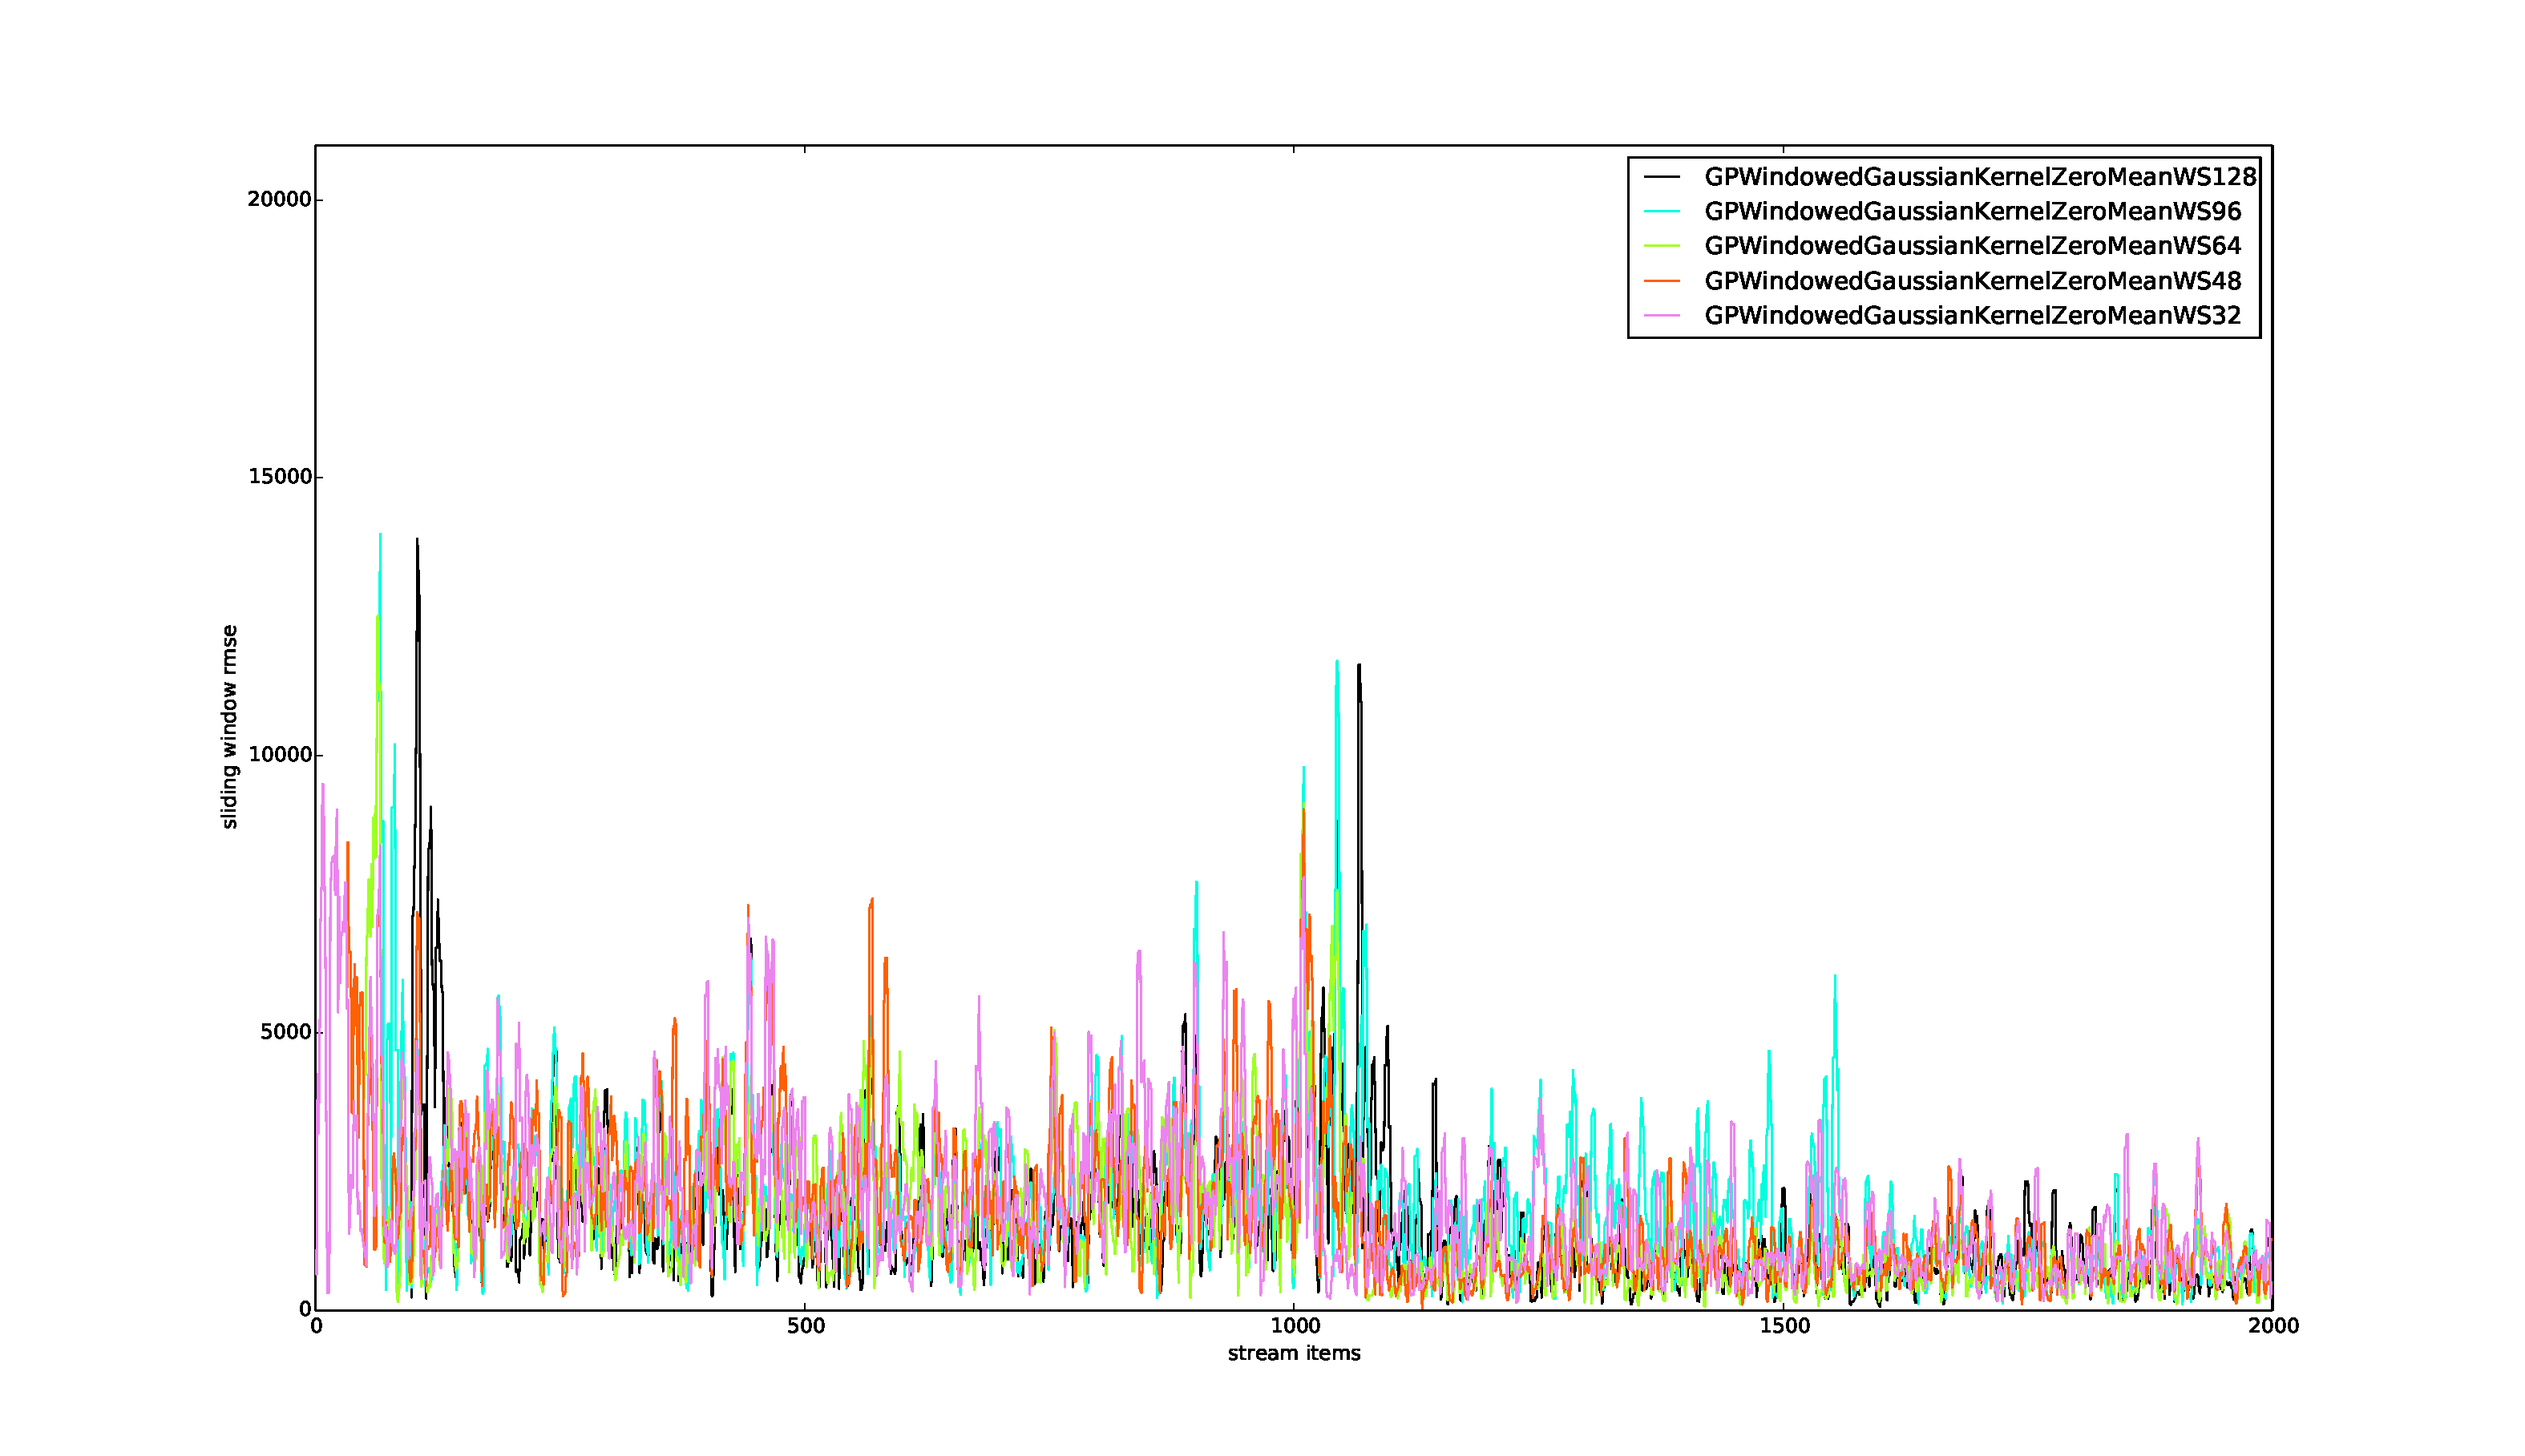
\includegraphics[width=\linewidth]{./Figures/wsize_on_stabilization2_sidebyside_comp_res4.pdf}
  \caption{Side-by-side Accuracy Comparison of \texttt{GPWindowedGaussianKernelZeroMean} variants with different window sizes. The test data used is \texttt{SYNTH\_D\_CD\_2000\_4\_10\_1\_24} and the resolution of the sliding error window accuracy evaluation method is set to 4}
  \label{fig:wsize_on_stabilization2_sidebyside_comp_res4}
\end{figure}

Another observation could be made from \ref{fig:wsize_on_stabilization_sidebyside_comp_res96} and \ref{fig:wsize_on_stabilization_sidebyside_comp_res4} is that the errors that the predictions of the online learner with the biggest window size contained during its unstable phase seems to be larger than that of the learners with smaller window sizes. However, this is an illusion of the sliding error window accuracy evaluation method employed for plotting the accuracy as a function of time. If we set the resolution parameter to a relatively low value, we do not get any clear picture of which learner have suffered from greater errors during their unstable phases as seen in \ref{fig:wsize_on_stabilization_sidebyside_comp_res4} and \ref{fig:wsize_on_stabilization2_sidebyside_comp_res4}.

\begin{figure}[htbp]
  \centering
    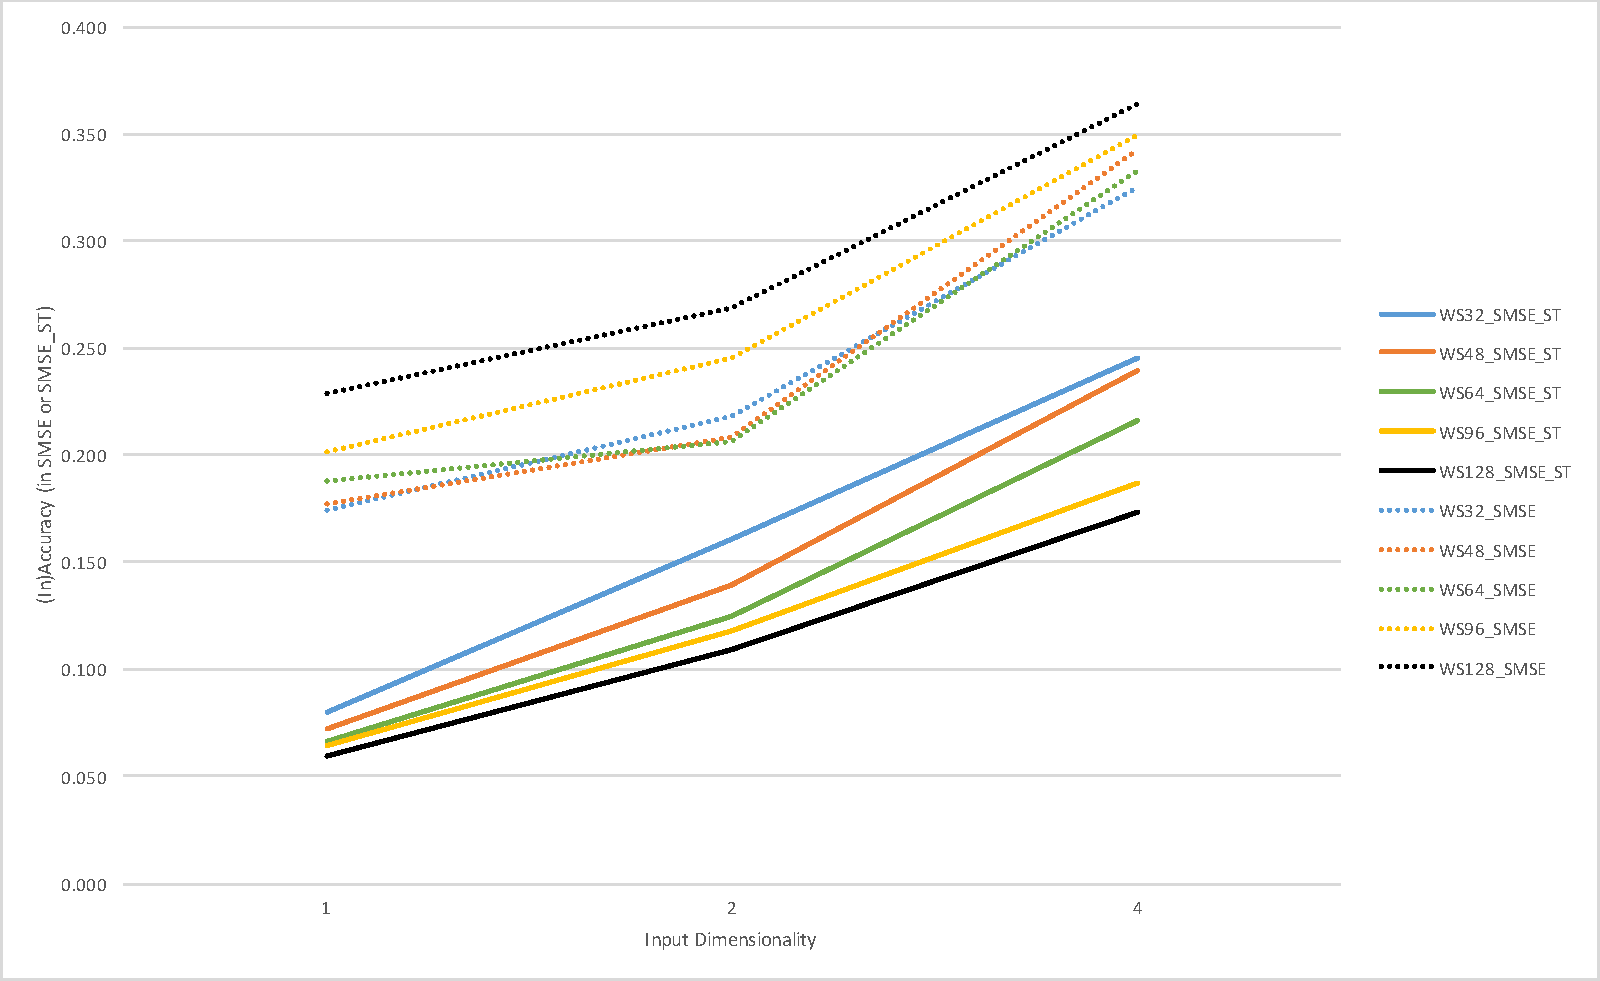
\includegraphics[width=\linewidth]{./Figures/curse_of_dim.pdf}
  \caption{Comparison of the increase in accuracy for different window sizes. \texttt{SMSE\_ST} values are aggregated over 576 stream simulations on 8 online learners (2 BayesianMAP, 2 BayesianMLE, 3 GPRegression and 1 KernelRegression variants) for each window size}
  \label{fig:curse_of_dim}
\end{figure}

Examining how the aggregate \texttt{SMSE\_ST} statistics change as the number of predictor variables increases. Figure \ref{fig:curse_of_dim} clearly shows that both statistics increase (meaning stable and total accuracy decreases) when there are more number of predictors. In the same figure, we also see that the learners with the smallest sliding window achieved a better stable accuracy on single dimensional data (one predictor) than the learners with the biggest sliding window on both two and four dimensional data. In other words, even though with the window size is increased from $36$ to $128$, when the number of dimensions are doubled, the accuracy drops. This suggests that increasing dimensions in the input space are not compensated by increasing the \textit{dynamic} training set as the same rate. This observation is a manifestation of \textit{Curse of Dimensionality}.

Similarly to \texttt{SMSE\_ST}, the change in \texttt{SMSE} results follow the same increasing pattern. However, as \texttt{SMSE} results are contaminated by the high errors during the unstable phases of online learners, drawing conclusions from them is less preferable to using \textit{SMSE\_ST} results if it is a relation between an environmental variable (e.g input dimensionality, input noise etc) and the accuracy in general that is being investigated. Nevertheless, \texttt{SMSE} results are also shown in \ref{fig:curse_of_dim} with by the dotted lines for the records.

The sliding window size affects the stream processing rate of online learners which are important considerations when learning from streams due to input-size dependent time complexity of learning algorithms. As described in \ref{Chapter5}, the lifecycle of an online learner featuring a sliding window is complex and depending on its state, it can take different amount of time to process a single stream item. This makes it harder to evaluate time-efficiency of the online learners. Thus, first a good time-efficiency evaluation strategy is discussed next, considering the variable state of the learners, then this strategy is applied to experiment data to make observations about the sliding window effects on the time-efficiency.

Whenever a significant error increase in the predictions is detected by its update mechanism, its update costs dominate its prediction cost (until it recycles one full window of data points and stabilizes) resulting in a significant amount of time spent on incorporating new points besides making predictions for new data points. This causes the average time to process data points to be higher than the average prediction time in the online algorithms in general. Thus, it can be argued that the pace at which an online learner with error-triggered update mechanism can learn is subject to changes. Therefore, when calculating the maximum data rate that it can learn from, its slowest processing speed should be taken into account. However, this would be a suitable time-efficiency evaluation strategy if the most naive approach dealing with streams is employed. A smarter one would be calculating the maximum stream rate according to the weighted average of the prediction, update and tuning times (weights being the number of times each operation took place until the point an evaluation is requested) and for the periods when the online learner is doing multiple operations on the incoming data stream items making use of a \textit{buffer} to be freed again once the online learner stabilizes on a concept and stops updating and tuning. Another sophisticated one would be using multi-threading to carry out update and tuning operations while new data points are arriving and being predicted. However, in this thesis, by assuming the availability of efficient stream buffering and multi-threading techniques to handle streams, for evaluating the consumption of time resources by the online learners, the weighted average of the prediction, update and tuning average is used as the criterion. In the testing setup employed, an easy way to compute the mentioned weighted average is simply to divide the total time spent on the stream by the learner by the number of data points\footnote{\label{not_violate_assumption}Note that this does not violate the \textit{possibly infinitely long} assumption of the data streams. only the number of stream items until an evaluation on the learner's performance is requested should be known to compute the weighted average.}. Thus, the time-efficiency metric \texttt{ATPI} is the major point of interest in the following time-efficiency analysis of the experiment data although in order to point out remarkable differences in prediction, update and tuning times separately between different learners with different algorithms and/or different window sizes \texttt{APT}, \texttt{TPT}, \texttt{AUT}, \texttt{TUT}, \texttt{ATT}, and \texttt{TTT} metrics are also used.

\begin{figure}[htbp]
  \centering
    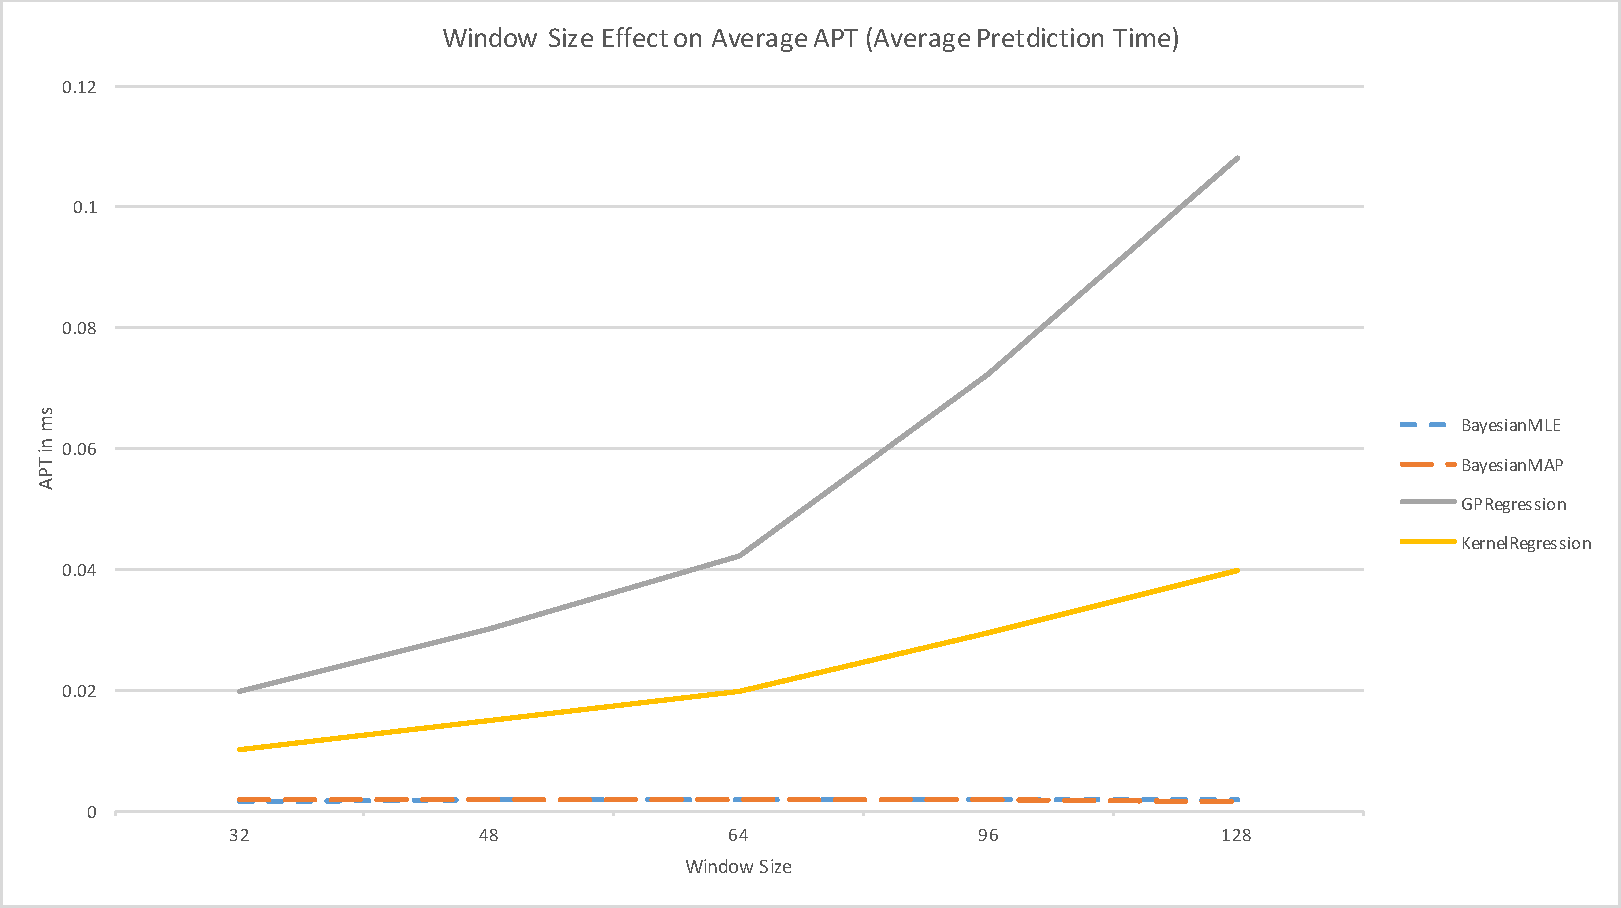
\includegraphics[width=\linewidth]{./Figures/ws_on_apt_per_alg.pdf}
  \caption{Comparison of the increase in average \texttt{APT} for different window sizes and algorithms. APT values are aggregated over 144, 216 and 216 streams which are simulated from data sets with 1,2 and 4 input dimensions respectively on 8 sliding windowed online learning algorithms for each window size}
  \label{fig:ws_on_apt_per_alg}
\end{figure}

\begin{figure}[htbp]
  \centering
    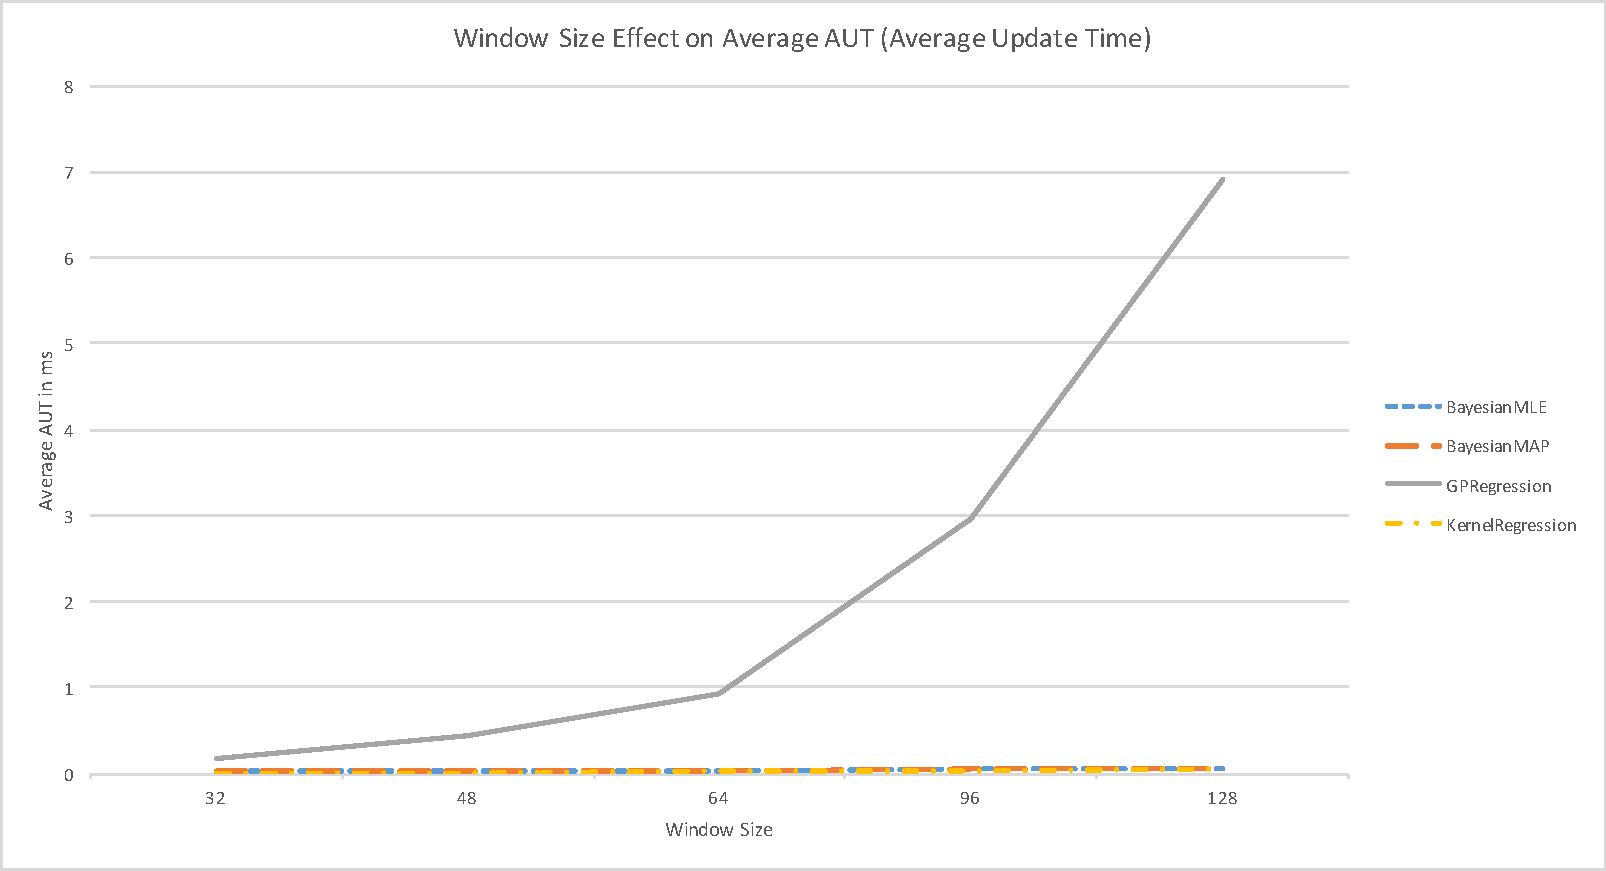
\includegraphics[width=\linewidth]{./Figures/ws_on_aut_per_alg.pdf}
  \caption{Comparison of the increase in average \texttt{AUT} for different window sizes and algorithms. APT values are aggregated over 576 stream simulations on 8 online learners (2 BayesianMAP, 2 BayesianMLE, 3 GPRegression and 1 KernelRegression variants) for each window size}
  \label{fig:ws_on_aut_per_alg}
\end{figure}

In \ref{fig:ws_on_apt_per_alg} and \ref{fig:ws_on_aut_per_alg}, we see how the average prediction time and the average update time respectively changes as the window size changes. Generally speaking, windows size comes at the cost of a slow-down in both prediction and update times however the amount of slow-down depends heavily on the algorithm choice. For example, \texttt{BayesianMLE} and \texttt{BayesianMAP} families are almost window-size insensitive in terms of prediction speed while \texttt{KernelRegression} and \texttt{GPRegression} learners exhibit a significant slow-down with larger window-sizes. As for the update speed, the amount of slow-down with all the algorithms but \texttt{GPRegression} are on the scale of $\mu$ seconds. On the other hand, \texttt{GPRegression} slow-down is measured in $m$ seconds making the points representing the average update time for all the algorithms except for \texttt{GPRegression} connect with an almost horizontal line. 

\begin{figure}[htbp]
  \centering
    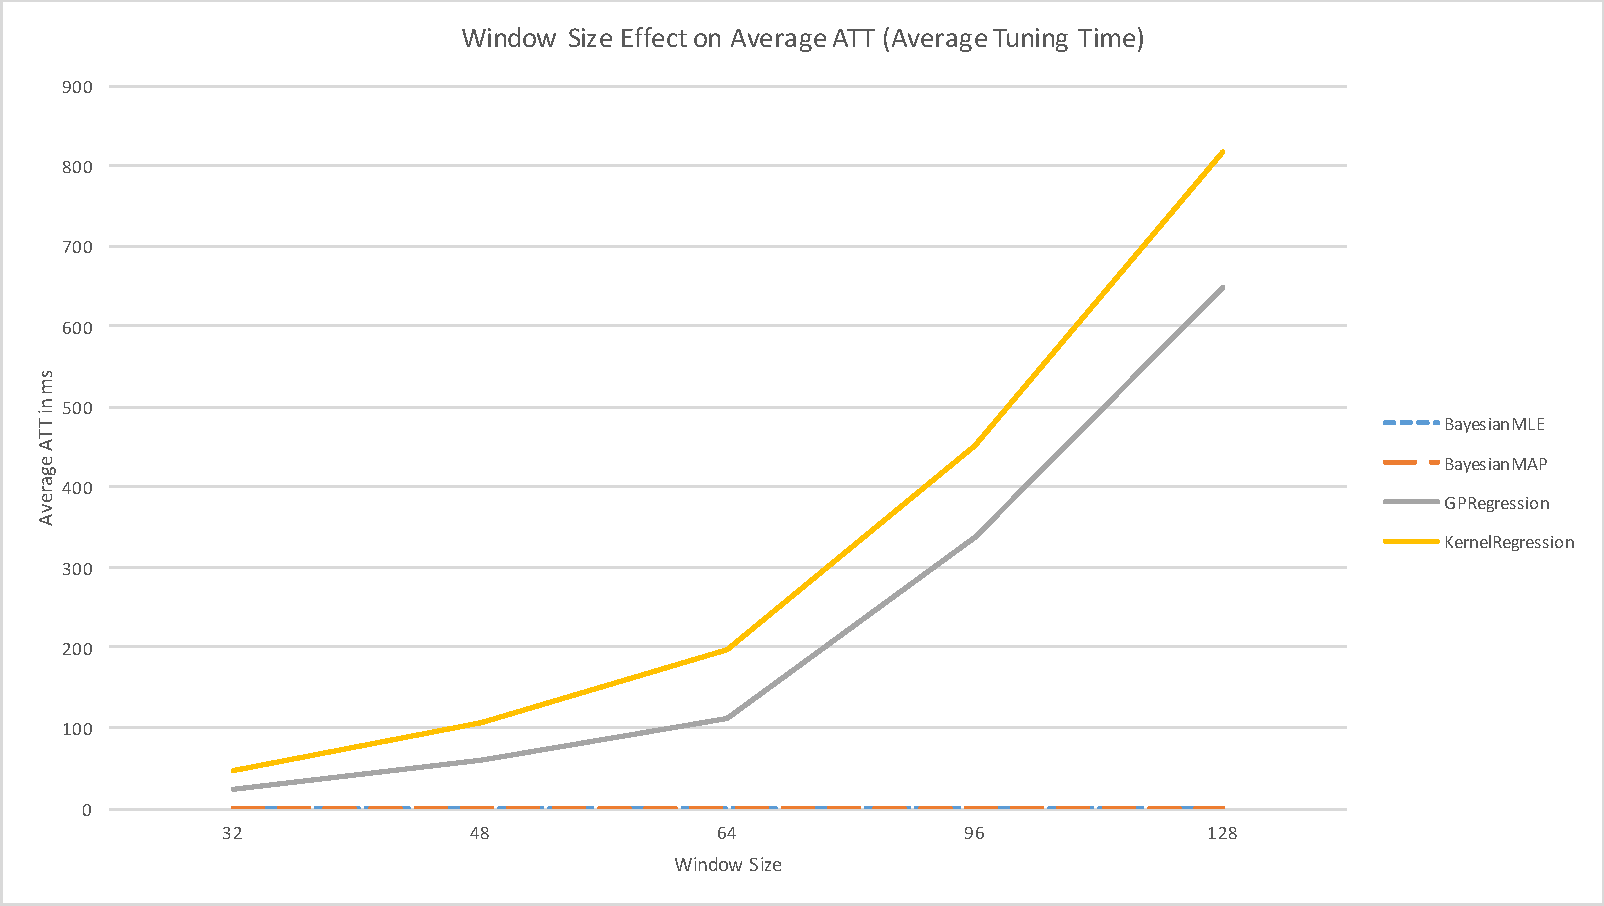
\includegraphics[width=\linewidth]{./Figures/ws_on_att_per_alg.pdf}
  \caption{Comparison of the increase in average \texttt{ATT} for different window sizes and algorithms. APT values are aggregated over 576 stream simulations on 8 online learners (2 BayesianMAP, 2 BayesianMLE, 3 GPRegression and 1 KernelRegression variants) for each window size}
  \label{fig:ws_on_att_per_alg}
\end{figure}

As the online learners with sliding window mechanism are tuned at least once after their window gets full and later conditional on the increasing error, tuning time is an important consideration. Figure \ref{fig:ws_on_att_per_alg} shows how the average \texttt{ATT} changes as the window size increases. \texttt{BayesianMLE} and \texttt{BayesianMAP} family learners appear to be insensitive to window size on the $ms$ scale. As for the learners using non-parametric algorithms exhibits a dramatic increase in their average tuning times. This is not surprising as explained in \ref{subsubsection:impl_tune_gpreg}, the tuning algorithm employed in \texttt{GPRegression} learners attempts to find the optimal hyperparameter configurations by manipulating the the gram-matrices that store as many items as the square of the number of items in the sliding window and as explained in \ref{subsubsection:impl_tune_kreg}, the tuning algorithm used by \texttt{KernelRegression} does a number of passes on the sliding-window which is proportional to the square of the sliding window size. On an important note, \texttt{KernelRegression} tuning routine takes more time than that of \texttt{GPRegression} according to averaged test results.

In order to see how each of the different operations, prediction, update and tuning, contributes to the total time spend by an online learner, a stacked column graph showing the breakdown of the total time spent is presented in \ref{fig:total_time_breakdown}. \texttt{GPRegression} and \texttt{KernelRegression} families spent substantial amount of time for tuning on average. As for \texttt{BayesianMLE} and \texttt{BayesianMAP} families, total time spent for tuning was negligible according to aggregated test results.

\begin{figure}[htbp]
  \centering
    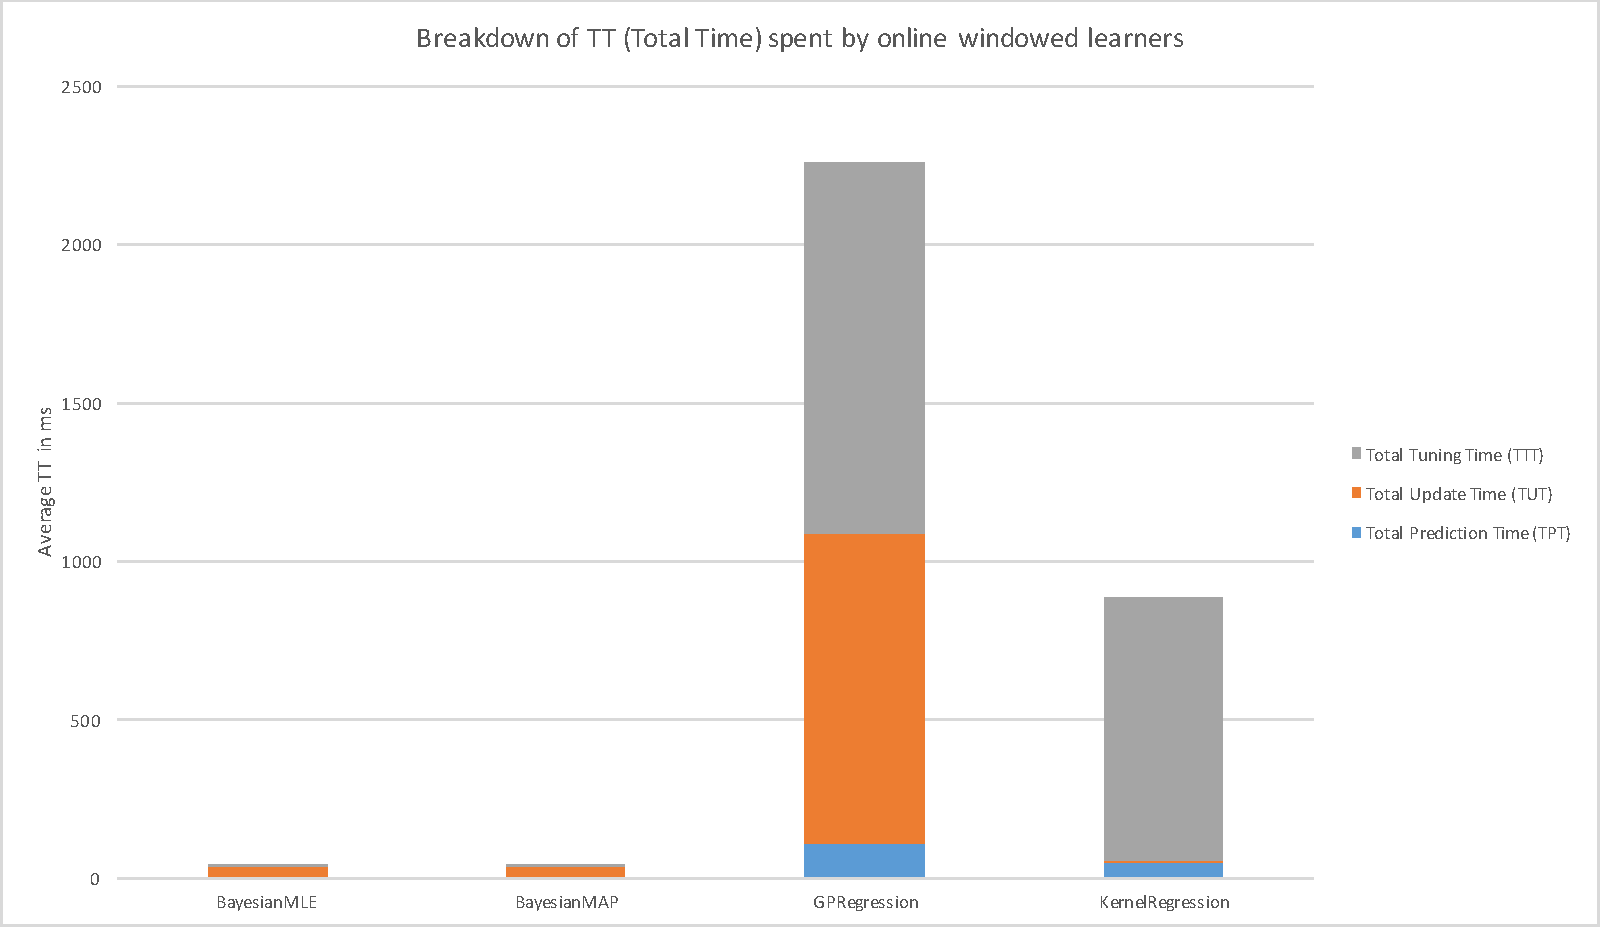
\includegraphics[width=\linewidth]{./Figures/total_time_breakdown.pdf}
  \caption{Average Total time spent per stream simulation shown as the summation of average prediction, update and tuning times. Sum of TPT, TUT and TTT are aggregated over 576 stream simulations on 6 BayesianMLE learners (2 variant parametrized with 3 window sizes), 6 BayesianMAP learners (2 variant parametrized with 3 window sizes), 9 GPRegression learners (3 variant parametrized with 3 window sizes) and 3 KernelRegression learners (Single variant parametrized with 3 window sizes)}
  \label{fig:total_time_breakdown}
\end{figure}

Having investigated how different window sizes affect different dimensions of the evaluation such as accuracy and the time efficiency, the conclusion about the window size to be made is that it has to be chosen very carefully. While with small window sizes, the high speed is guaranteed, big window size does not guarantee higher general accuracy always. Nevertheless, there is a sweet point between high window sizes and low window sizes that need to be picked in order to achieve a good accuracy without suffering from substantial slow-down that prevents the algorithm to be employed from the stream learning scenarios. However, where this sweet point lies depends on the algorithm choice. 

\subsubsection{\texttt{GPRegression} Window Size}
\label{section:gp_reg_win_size}

As shown in \ref{fig:ws_on_gpreg_tt}, total time spent by the \texttt{GPRegression} learners grows with the increasing window size. \texttt{ATPI} statistic which can be used to calculate the maximum data rate an online learner can handle as explained previously is obtained by simply dividing the \texttt{TT} by the number of data points appeared in the stream until the performance evaluation of the online learner is requested. In the test setup, the streams are simulated from $2000$ data points, in this case, if \texttt{TT} is known, \texttt{ATPI},  maximum data rate, denoted as \texttt{DRmax} and measured in items per $ms$ can be handled by an online learner, can be obtained using the following formula.
\begin{flalign} 
& \texttt{ATPI} = \frac{\texttt{TT}}{2000} \\
& \texttt{DRmax} = \texttt{ATPI}^{-1}
\end{flalign}

\begin{figure}[htbp]
  \centering
    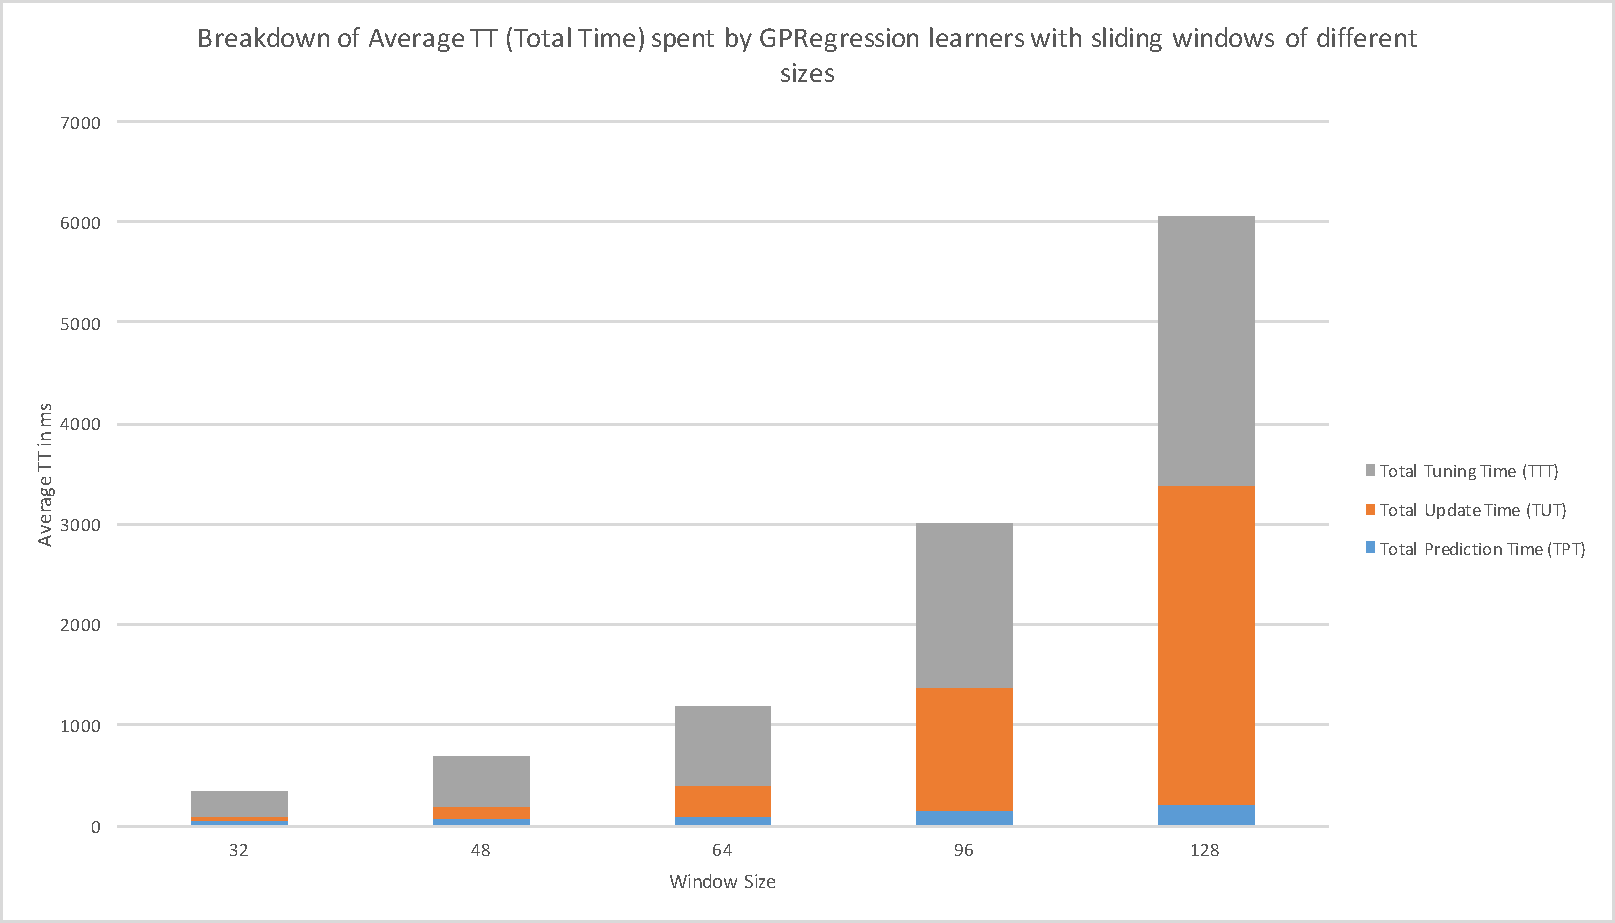
\includegraphics[width=\linewidth]{./Figures/ws_on_gpreg_tt.pdf}
  \caption{Average Total time spent per stream simulation shown as the summation of average prediction, update and tuning times. Sum of TPT, TUT and TTT are aggregated over 576 stream simulations on 3 KernelRegression variants for each different window sizes)}
  \label{fig:ws_on_gpreg_tt}
\end{figure}

\begin{figure}[htbp]
  \centering
    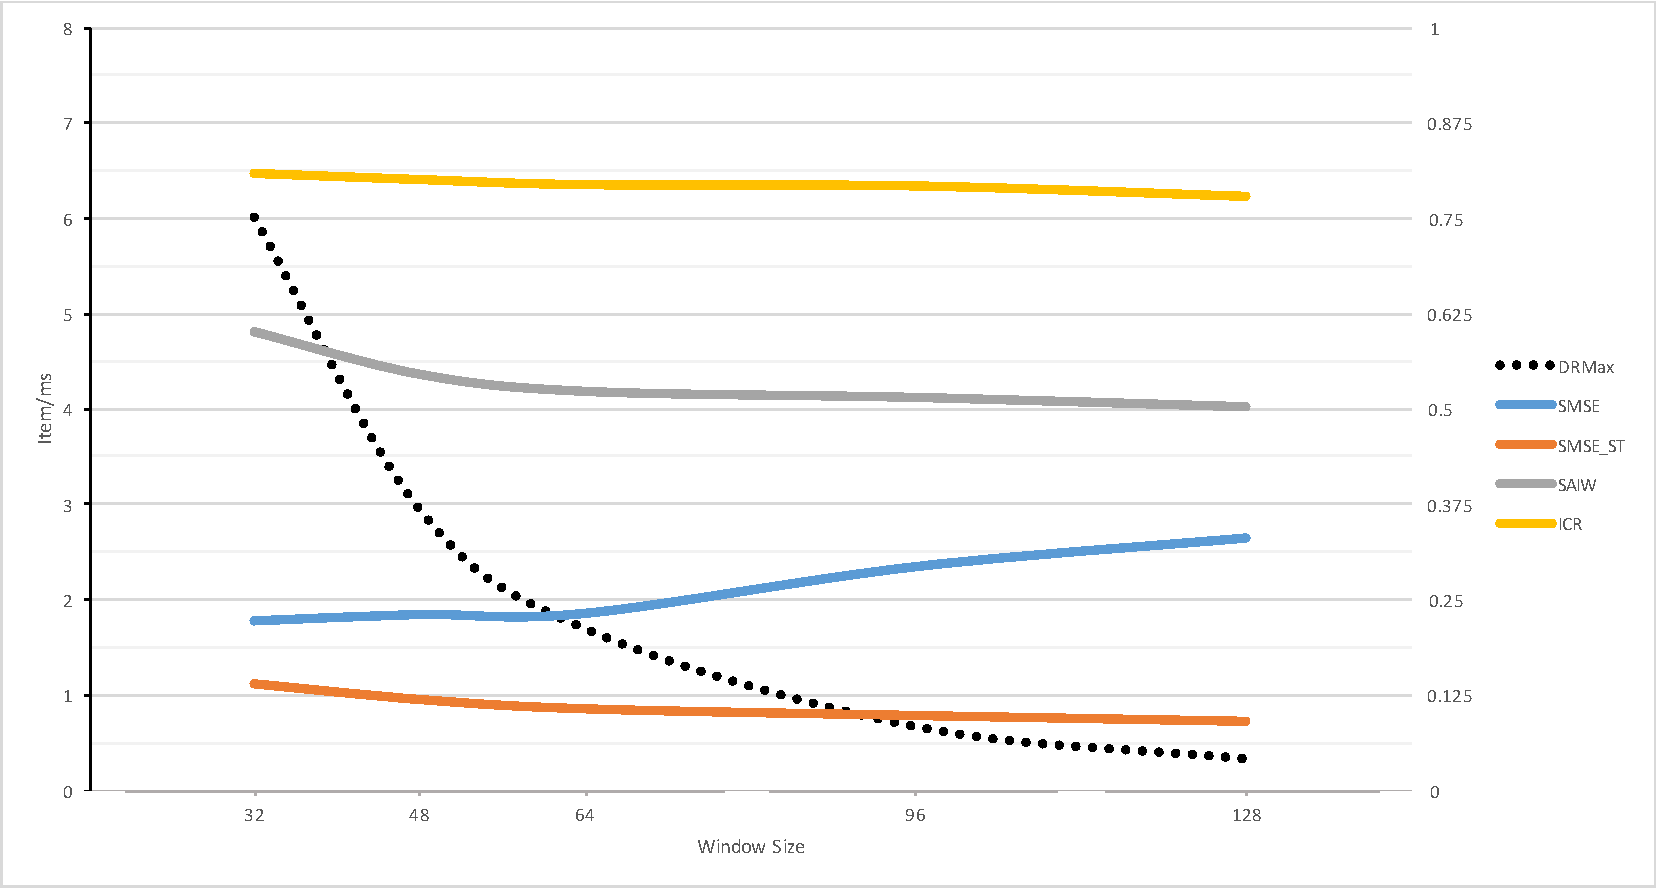
\includegraphics[width=\linewidth]{./Figures/gpreg_wsize_sweet_pt.pdf}
  \caption{Average \texttt{DRmax}, \texttt{SMSE}, \texttt{SMSE\_ST}, \texttt{SAIW} and \texttt{ICR} scores for \texttt{GPRegression} learners are graphed. First statistic \texttt{DRmax} uses the primary axis with the interval $[0,8]$ while the rest use the secondary y- axis with the $[0,1]$ interval. The statistics are aggregated from 576 stream simulations on 3 KernelRegression variants for each different window sizes)}
  \label{fig:gpreg_wsize_sweet_pt}
\end{figure}

Applying above formula to the \texttt{GPRegression} learners to obtain the average \texttt{DRMax} scores of them over different tests and three different variants of \texttt{GPRegression} and using the average \texttt{SMSE} presented previously, we get Figure \ref{fig:gpreg_wsize_sweet_pt} which helps spot the sweet point for the size of the sliding window that \texttt{GPRegression} learners have. The figure indicates that the prediction bound coverage are nearly the same for all the window sizes. In terms of the average width of prediction bounds, all the window sizes produced reasonably sized bounds although the prediction bounds of the learners with the smallest choice of window size was a bit larger than the rest. Having verified that prediction bounds and their coverage are good for all window sizes, the trade-off between accuracy and the maximum data rate can be handled is the major consideration to pick a good window size. 

In the same graph, we see that there is actually no trade-off between the general accuracy \texttt{SMSE} and \texttt{DRmax}. The smallest window size appears to dominate the other window sizes by providing the lowest \texttt{SMSE} and highest \texttt{DRmax} values. However, when evaluating the \texttt{SMSE} scores one should keep in mind that in addition to the window size, the general accuracy scores depend on the number of concept drifts and the number of stream items arrived until the moment online learner performance statistics are computed in the lifetime of the stream. In the stream simulations, these parameters are all fixed. As explained previously in this chapter, half of the stream simulations feature an abrupt concept drift at the $1000_{th}$ data point. In a real-life stream learning scenario, it is not possible to know how many concept changes how frequently will occur. Therefore, instead of \texttt{SMSE}, looking at the \texttt{SMSE\_ST} scores which is a measure of the stable (in)accuracy while still keeping in mind that high window sizes have longer adaptation times is better when finding the sweet point for the window sizes. 

When the \texttt{SMSE\_ST} scores are examined in \ref{fig:gpreg_wsize_sweet_pt}, there indeed seems to be a true trade-off between the stable accuracy and maximum data rate. Higher the stable accuracy is lower the maximum data rate is. The highest window sizes namely $96$ and $128$ having the superior stable accuracy to the other window sizes can handle streams up to approximately $0.33$ and $0.67$ items per millisecond. Since, the Ocelot runtime predictor is expected to get performance estimation requests once in a millisecond on average, window size of $96$ and $128$ are not good choices. After $96$ and $128$, the window size choice of $64$ has the best stable accuracy and it allows to process stream items approximately at $1.69$ items per millisecond meeting the data rate requirement. Therefore, the sweet point for the window size choice in \texttt{GPRegression} learners is determined to be $64$.

\subsubsection{\texttt{KernelRegression} Window Size}

For \texttt{KernelRegresison} learners, Figure \ref{fig:ws_on_kreg_tt} allows for a detailed analysis on their time-efficiency. Similarly to \texttt{GPRegression} learners, the average total time spent grows with the increasing window size although differently from \texttt{GPRegression} the biggest contribution to the total time spent is from the tuning costs. Also similarly to \texttt{GPRegression}, the average \texttt{ICR} scores appear to be insensitive to the window size choice. However, they show that the interval coverage rate of \texttt{KernelRegression} is not sufficient. Nevertheless, when deciding for a good window size, this deficiency is not considered and in the next section a good workaround for it is proposed. As for the average \texttt{SAIW} scores, except for the lowest choice of window size $32$, they seem to be pretty low meaning that prediction bounds were tight which is a desirable result in general. Moreover, with the highest window size option $128$, \texttt{SAIW} shows prediction bounds were even tighter.

\begin{figure}[htbp]
  \centering
    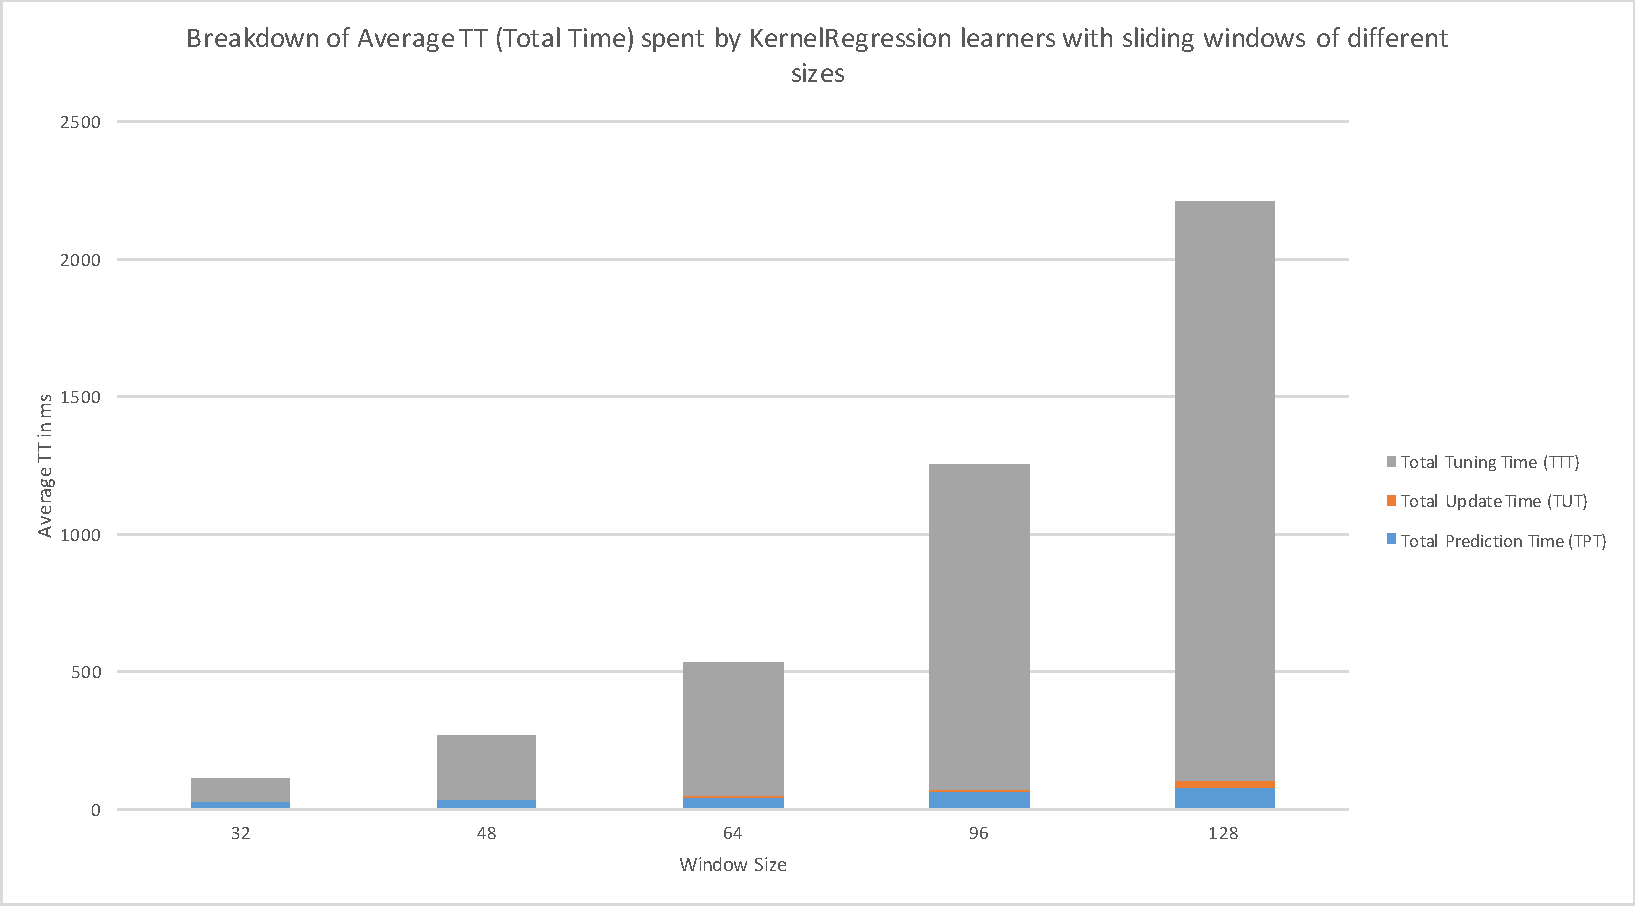
\includegraphics[width=\linewidth]{./Figures/ws_on_kreg_tt.pdf}
  \caption{Average Total time spent per stream simulation shown as the summation of average prediction, update and tuning times. Sum of TPT, TUT and TTT are aggregated over 576 stream simulations on the only existing KernelRegression variant for each different window sizes)}
  \label{fig:ws_on_kreg_tt}
\end{figure}

The discussion in \ref{section:gp_reg_win_size} regarding the choice between \texttt{SMSE} and \texttt{SMSE\_ST} as the (in)accuracy criteria also holds here. When the average \texttt{SMSE\_ST} and \texttt{DRmax} scores are compared between different window sizes, performance-accuracy trade-off catches attention. Simply, the higher stable accuracy, lower the maximum data rate can be handled. \texttt{GPRegression} learners with the largest window size choice $128$ can process stream items approximately at $0.95$ items per millisecond. This is just below the expected data rate in Ocelot operator runtime performance behavior. Also considering the evident late-stabilization times that large-windowed learners have, the largest window size among the other options is not the best choice. The second biggest window-size among the available options $96$ can handle stream items arriving $1.69$ items per millisecond making it employable for Ocelot operator runtime predictor.
\begin{figure}[htbp]
  \centering
    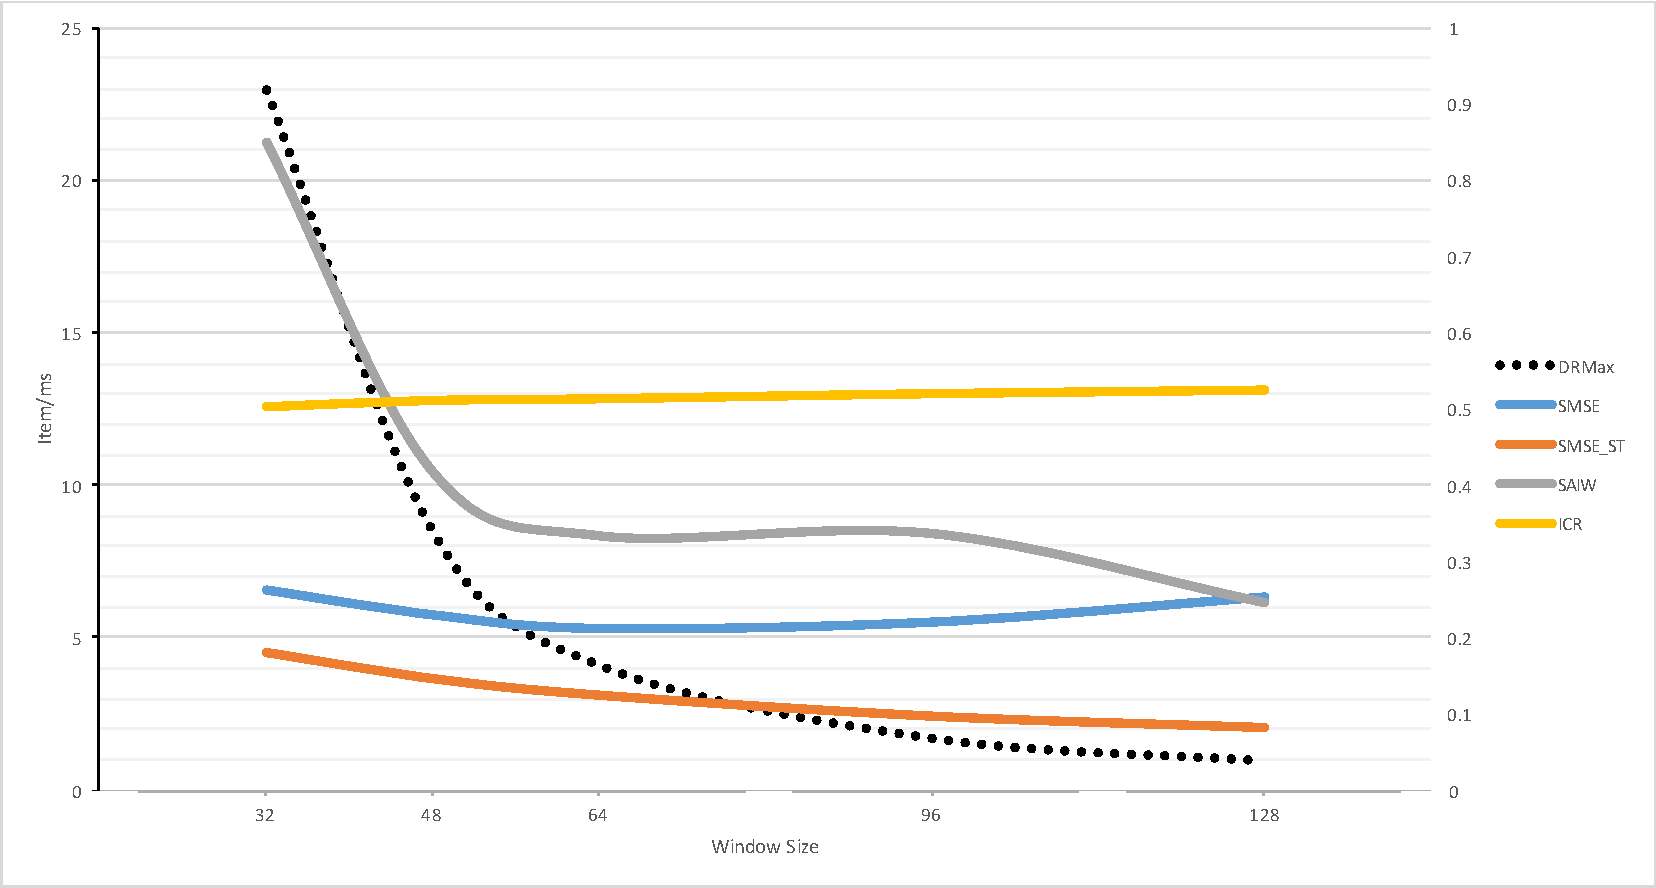
\includegraphics[width=\linewidth]{./Figures/kreg_wsize_sweet_pt.pdf}
  \caption{Average \texttt{DRmax}, \texttt{SMSE}, \texttt{SMSE\_ST}, \texttt{SAIW} and \texttt{ICR} scores for \texttt{GPRegression} learners are graphed. First statistic \texttt{DRmax} uses the primary axis with the interval $[0,25]$ while the rest use the secondary y- axis with the $[0,1]$ interval. The statistics are aggregated from 576 stream simulations on 3 KernelRegression variants for each different window sizes)}
  \label{fig:kreg_wsize_sweet_pt}
\end{figure}

When the biggest window size among the available options are employed, KernelRegression is still quicker than the GPRegression with the window size of $64$. Despite this, it may not be the best option to stick with the largest choices for the window size due to the accuracy problems that sliding windowed algorithms with big windows have more during their are unstable periods than their smaller windowed versions. Hence, the preferred window sizes for the \texttt{KernelRegression} is $64$ and $96$.

\subsubsection{\texttt{BayesianMLE} and \texttt{BayesianMAP} Window Size}

Although the same relation between the window size and the total time spent observed in parametric learners is also present in the case of non-parametric learners, in \ref{fig:ws_on_bmle_bmap_tt}, we see that even the learners with the window size of $128$ is way quicker than their counterparts from other algorithms with the window size of $32$. As a result, the streams that can be handled with parametric learners can be way faster. For example, \texttt{BayesianMAP} learner with the sliding window of $128$ data points can handle streams up to $(\frac{57.87}{2000})^{-1}\approx 34.56$ items per millisecond. Therefore, performance-wise, any window-size from 32 to 128 is fine for \texttt{BayesianMLE} and \texttt{BayesianMAP} to be employed as the runtime predictor module in Ocelot.

\begin{figure}[htbp]
  \centering
    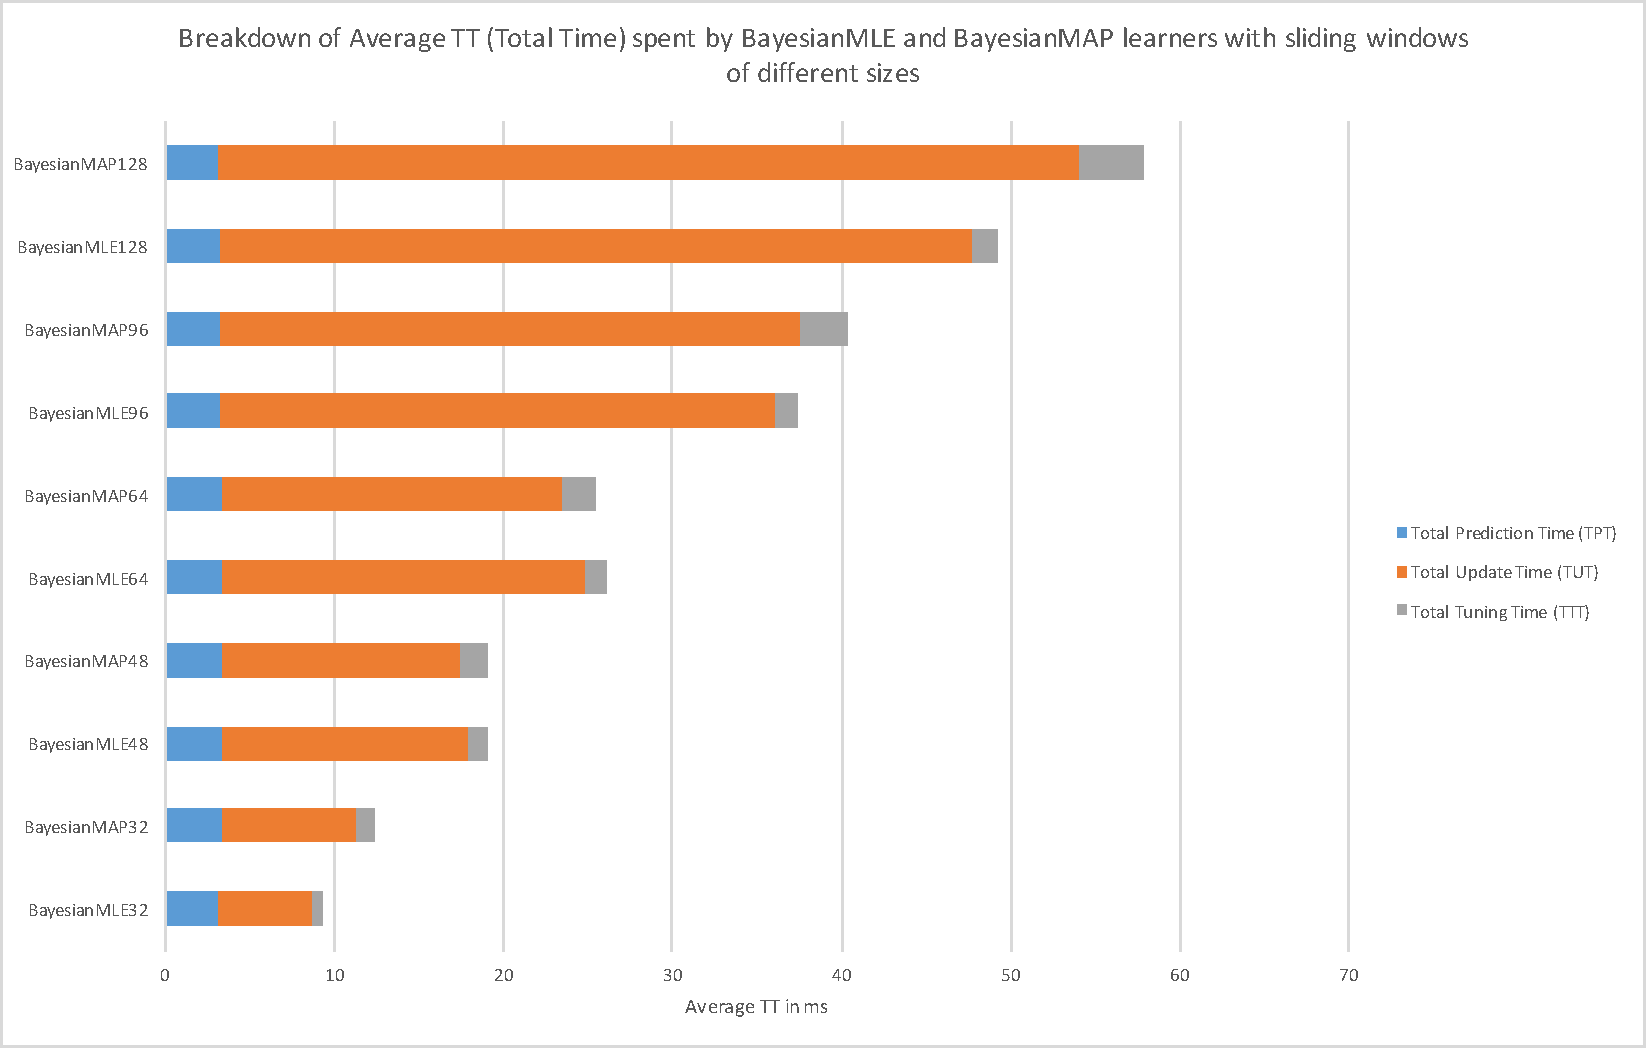
\includegraphics[width=\linewidth]{./Figures/ws_on_bmle_bmap_tt.pdf}
  \caption{Average Total time spent per stream simulation shown as the summation of average prediction, update and tuning times. Sum of TPT, TUT and TTT are aggregated over 576 stream simulations on 2 BayesianMLE and 2 BayesianMAP variants with three different window sizes each)}
  \label{fig:ws_on_bmle_bmap_tt}
\end{figure}

\begin{figure}[htbp]
  \centering
    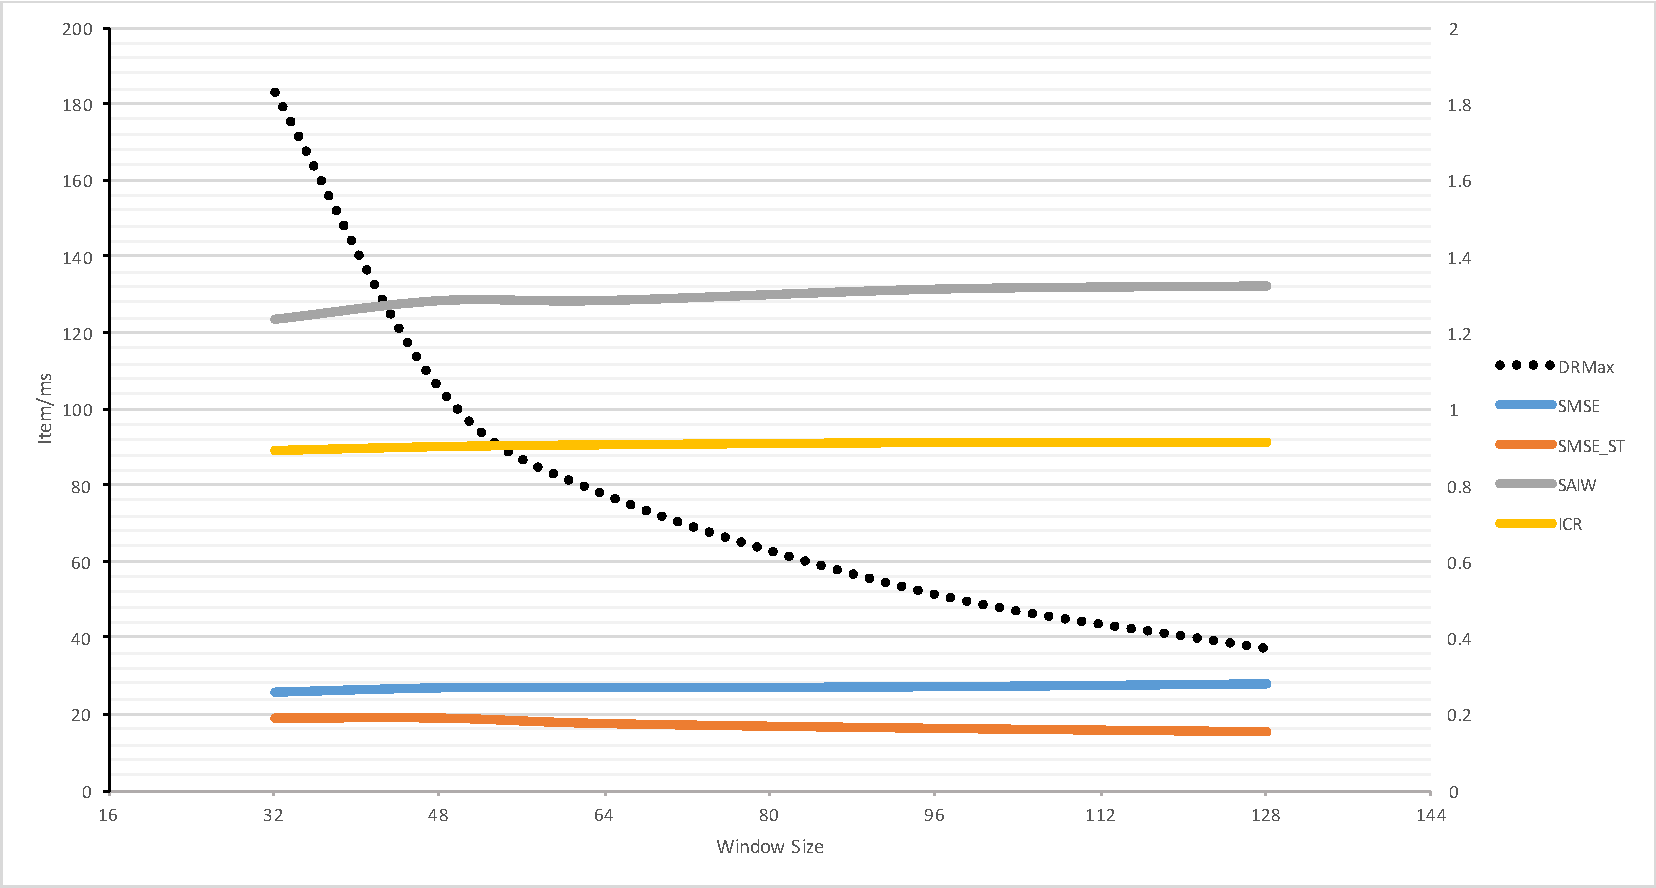
\includegraphics[width=\linewidth]{./Figures/bmle_bmap_sweet_pt.pdf}
  \caption{Average \texttt{DRmax}, \texttt{SMSE}, \texttt{SMSE\_ST}, \texttt{SAIW} and \texttt{ICR} scores for \texttt{GPRegression} learners are graphed. First statistic \texttt{DRmax} uses the primary axis with the interval $[0,200]$ while the rest use the secondary y- axis with the $[0,2]$ interval. The statistics are aggregated from 576 stream simulations on 2 \texttt{BayesianMLE} and 2 \texttt{BayesianMAP} variants for each different window sizes)}
  \label{fig:gpreg_wsize_sweet_pt}
\end{figure}

In terms of prediction bound related statistics namely \texttt{ICR} and \texttt{SAIW}, window size appeared to have no effect. Therefore, these metrics are not considered when choosing the window-size.

Since all the window sizes offer satisfactory processing speeds, there is no trade-off between the accuracy and the performance. One can simply opt for the the window size that affords the best performance. However, the inherited unstable phase accuracy drop problem is more troublesome with the larger window sizes similar to any other sliding-windowed learner. Therefore, it is not wisest choice to opt for the highest window size possible. Thus the moderate sizes such as $64$ and $96$ are considered for the further evaluation.

\subsection{Forgetting-factor}

A similar parameter to the sliding window size for the online learners that do not feature a sliding window is the forgetting factor. Out of 52 online learner, 12 use a forgetting mechanism to adapt to potential concept drifts. Similar to sliding-windowed approaches, the forgetting factor, being the essential parameter in forgetting-factor based learners is expected to affect the evaluation metrics. In order to discover how it affects the learning performance (accuracy, time costs, prediction bounds quality) of the forgetting-windowed learners, the figure \ref{fig:bmle_bmap_ff_sweet_pt} is prepared.

\begin{figure}[htbp]
  \centering
    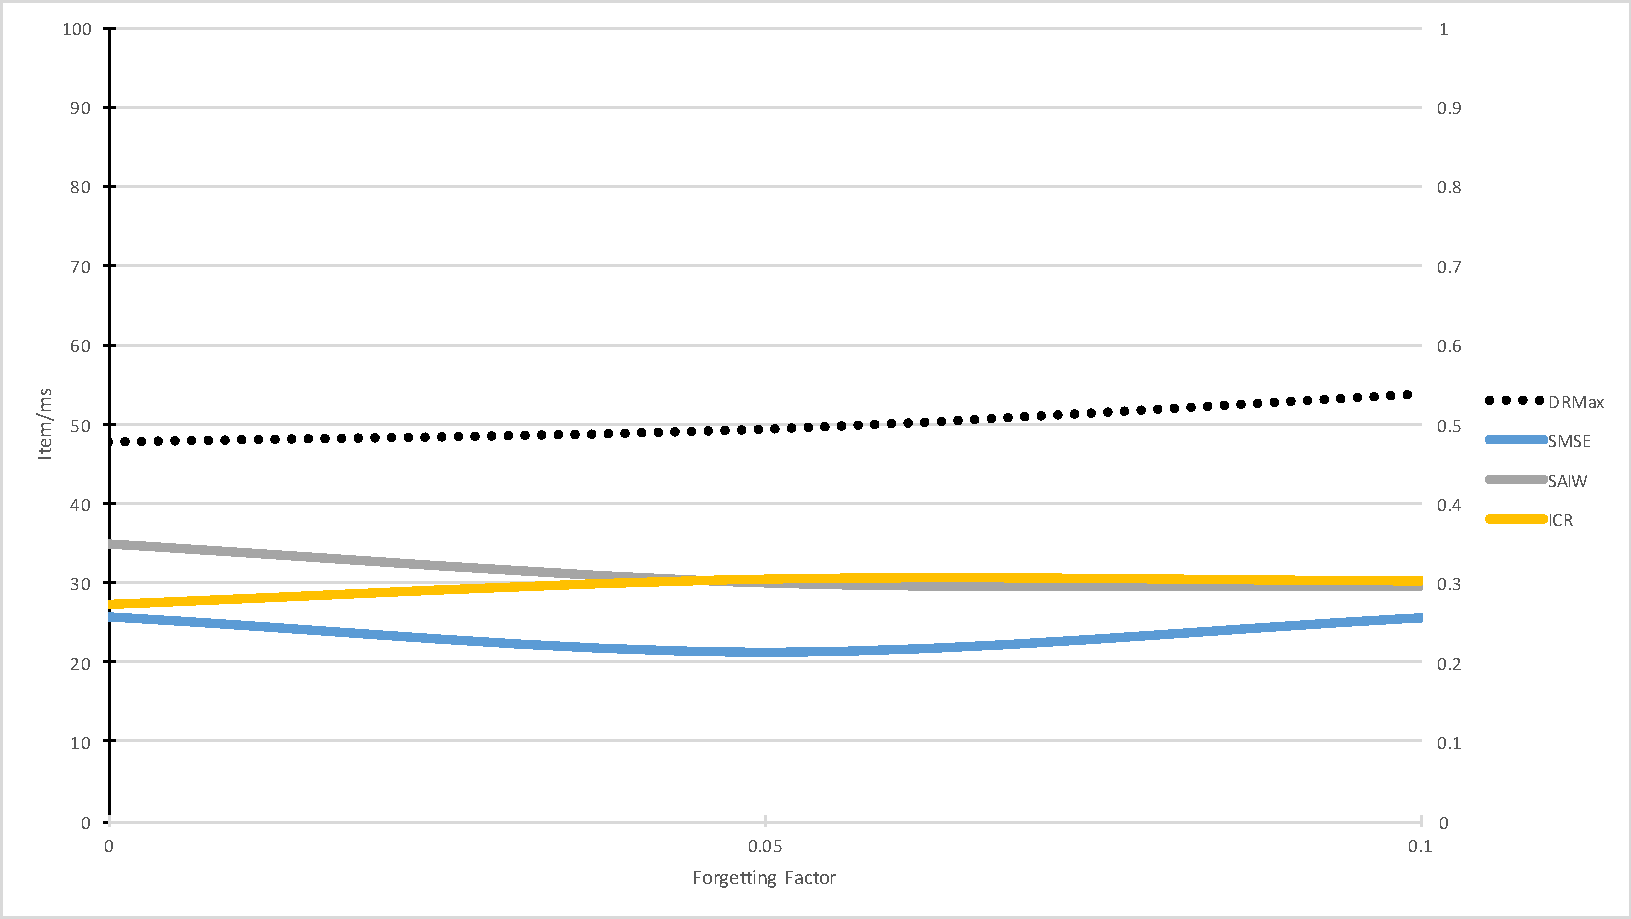
\includegraphics[width=\linewidth]{./Figures/bmle_bmap_ff_sweet_pt.pdf}
  \caption{Average \texttt{DRmax}, \texttt{SMSE}, \texttt{SAIW} and \texttt{ICR} scores for \texttt{BayesianMAP} and \texttt{BayesianMLE} learners are graphed. First statistic \texttt{DRmax} uses the primary axis with the interval $[0,100]$ while the rest use the secondary y- axis with the $[0,1]$ interval. The statistics are aggregated from 576 stream simulations on 2 \texttt{BayesianMLE} and 2 \texttt{BayesianMAP} variants for each forgetting factors)}
  \label{fig:bmle_bmap_ff_sweet_pt}
\end{figure}

According to the test results presented in the graph, the average prediction bounds scores namely \texttt{SAIW} and \texttt{ICR} were almost the same for the forgetting factors $0.05$ and $0.1$. For the $0$, the average \texttt{SAIW} was higher and the average \texttt{ICR} was lower than those of the learners with other forgetting factors although the differences were not significantly high. As for the performance implications, the change in forgetting factor did not cause a remarkable change in the maximum data rate can be handled.

The evaluation dimensions such as time-efficiency and the prediction bounds did not give a clue which forgetting factor is a better choice. In terms of the accuracy, similarly to the window-size parameter, there seems to be a sweet point for the forgetting factor to be chosen. Among the three forgetting factor choices used in the experiments namely $0$, $0.05$ and $0.1$, the forgetting factor of $0.05$ proved to be the best choice in terms of the accuracy\footnote{Note that there is no distinction of stable and general accuracy in the case of online learners not featuring a sliding window} of the predictions that the learners produced. This is not surprising since at the lower end using $0$ as the forgetting factor means not allowing algorithm to forget anything which obviously makes the adaptation of algorithm to the new concepts last forever. Setting forgetting-factor too high would result in underfacilitating the training examples that the online learner has observed making the algorithm always undertrained. 

As a result, when the experiment data is analyzed, it is observed that the sweet point for the forgetting factor lies somewhere in between $0.0$ and $0.1$. Thus, the forgetting factor $0.05$ works best among the available forgetting factor options.

\subsection{Feature Space Mapping}

As explained in Chapter \ref{Chapter4}, learners using a parametric learning algorithm have the option to map the input data point to a feature space which has a higher dimensionality than the input space. In the subsection, the implications of the feature space mapping on the evaluation criteria namely accuracy, prediction bounds and time-efficiency are discussed.

\begin{figure}[htbp]
  \centering
    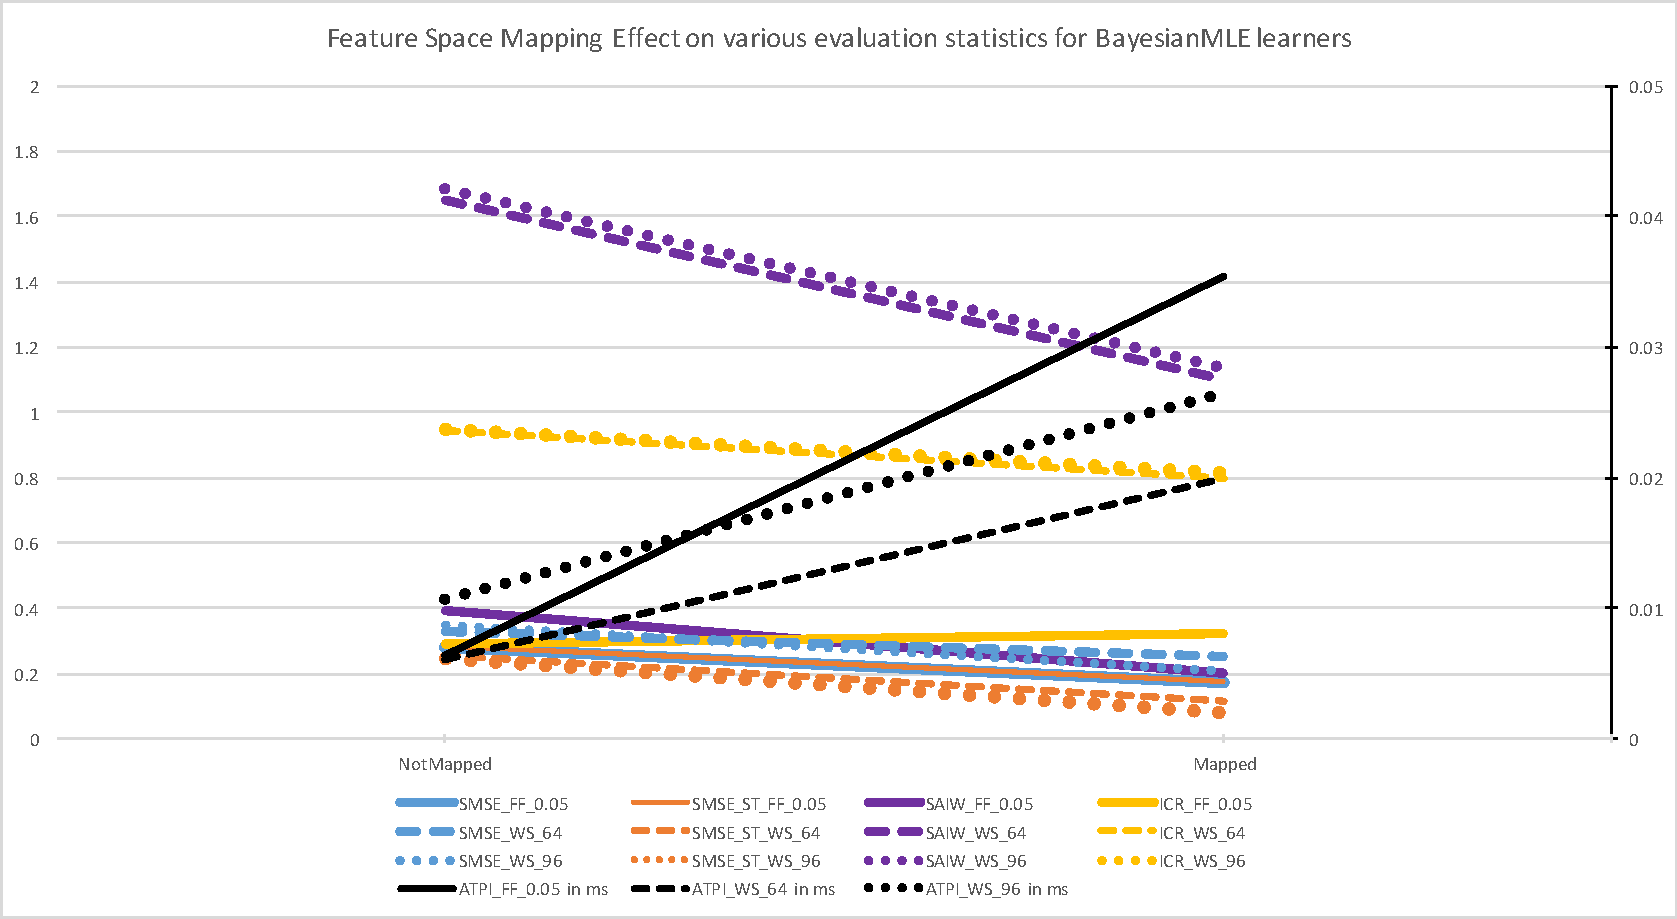
\includegraphics[width=\linewidth]{./Figures/fsm_effect_bmle.pdf}
  \caption{\texttt{SMSE}, \texttt{SAIW},\texttt{ICR} and \texttt{ATPI} scores for 6 different \texttt{BayesianMLE} learners are graphed. \texttt{ATPI} scores measured with respect to the secondary y-axis with the interval $[0,0.005]$ while the rest use the primary y-axis with the $[0,2]$ interval. The statistics are aggregated from 576 stream simulations on \texttt{BayesianMLEForgetting\_FF0.05}, \texttt{BayesianMLEWindowed\_WS64} and \texttt{BayesianMLEWindowed\_WS96} learners (each having one mapped and one non-mapped version)}
  \label{fig:fsm_effect_bmle}
\end{figure}

In Figure \ref{fig:fsm_effect_bmle}, how feature space mapping affects the accuracy, prediction bounds quality and time-efficiency of \texttt{BayesianMLE} learners with the window sizes and forgetting factors chosen in the previous subsections is shown. Except for \texttt{ICR}, feature space mapping has affected the other statistics in the same way for all the \texttt{BayesianMLE} learners analyzed to discover feature space mapping implications. \texttt{SMSE}, \texttt{SMSE\_ST} and \texttt{SAIW} appear to be lower when the feature space mapping is employed. This means, feature-space mapping boosts accuracy and tightens the prediction bounds. In terms of the time-efficiency, feature-space mapping has increased the \texttt{ATPI} meaning that more processing time per stream item is needed with the feature-space mapping. However, the average increased processing times for all the learners considered in the figure are all still below $0.04$ millisecond which is still way lower than that of than non-parametric models.  As for \texttt{ICR}, feature-space mapping caused a slight drop in the case of windowed learners making the coverage of the prediction bounds lower prediction bound coverage. However, the \texttt{ICR} values when the feature space is enabled is above $0.8$ for the windowed learners considered in the graph meaning that with feature space mapping, the the prediction bounds coverage of the unobserved targets are still satisfactory. As for the only forgetting factor variant considered, feature-space mapping has improved its interval coverage although the difference is negligible.

Feature-space mapping is observed to boost accuracy and tighten the prediction bounds while keeping the prediction bound coverage at the acceptable levels. This comes at the cost of slight increase in the average processing time. Having also observed that the mapped \texttt{BayesianMLE} learners are still way faster than what is required (all the mapped versions considered can process data streams faster than $25$ item per ms while the requirement is set to be around $1$ item per ms), \texttt{BayesianMLE} learners with feature-space mapping are preferred over their counterparts not featuring feature-space mapping.

\begin{figure}[htbp]
  \centering
    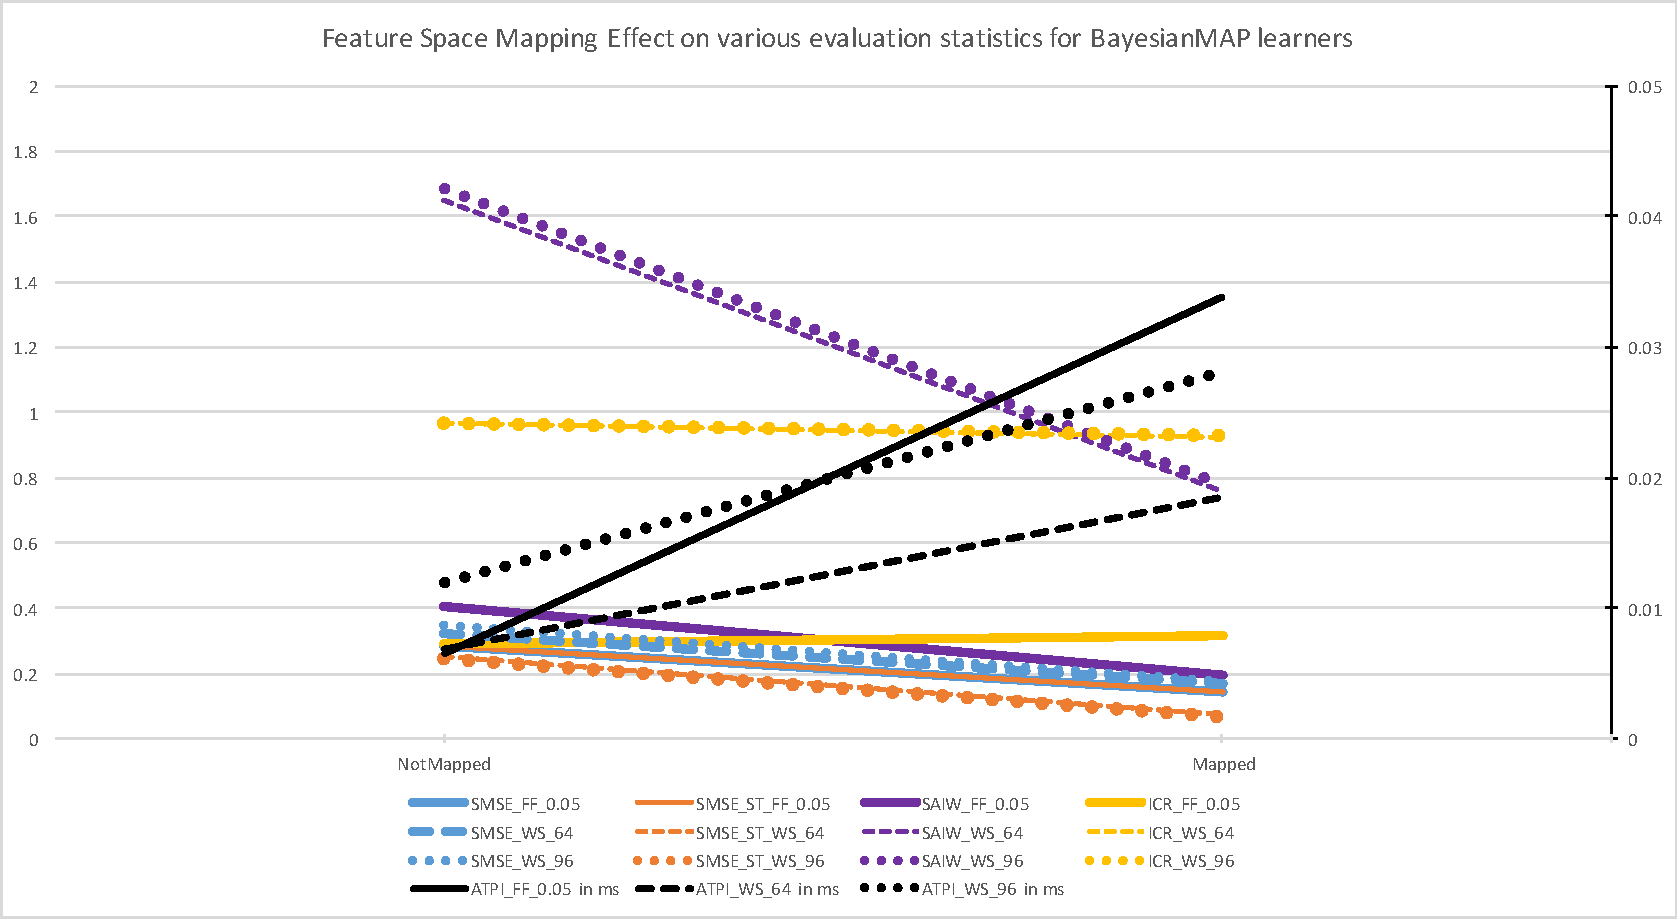
\includegraphics[width=\linewidth]{./Figures/fsm_effect_bmap.pdf}
  \caption{\texttt{SMSE}, \texttt{SAIW},\texttt{ICR} and \texttt{ATPI} scores for 6 different \texttt{BayesianMLE} learners are graphed. \texttt{ATPI} scores measured with respect to the secondary y-axis with the interval $[0,0.005]$ while the rest use the primary y-axis with the $[0,2]$ interval. The statistics are aggregated from 576 stream simulations on \texttt{BayesianMLEForgetting\_FF0.05}, \texttt{BayesianMLEWindowed\_WS64} and \texttt{BayesianMLEWindowed\_WS96} learners (each having one mapped and one non-mapped version)}
  \label{fig:fsm_effect_bmap}
\end{figure}

In Figure \ref{fig:fsm_effect_bmap}, how feature space mapping affects the accuracy, prediction bounds quality and time-efficiency of \texttt{BayesianMAP} learners with the window sizes and forgetting factors chosen in the previous subsections is shown. The same patterns observed as in the relation between the feature-space mapping and the accuracy, prediction bounds and time-efficiency scores appeared for the \texttt{BayesianMLE} learners. Briefly, feature-space mapping has improved the accuracy and without sacrificing a good coverage of the prediction bounds, it tightens them. In return, the average time needed for processing a single data stream item increased although this does not change the employability of the considered \texttt{BayesianMAP} learners with the feature-space mapping. Thus, the option of feature-space mapping is opted in for the considered \texttt{BayesianMAP} namely \texttt{BayesianMAPForgetting\_FF0.05}, \texttt{BayesianMAPWindowed\_WS64} and \texttt{BayesianMAPWindowed\_WS96}.

\subsection{Algorithm comparison}

Having uncovered the effect of sliding window size and forgetting-factor parameters on the qualities of the predictions such as accuracy, prediction bounds quality and time-efficiency and picking more preferable choices for these parameters, now a more detailed comparison of the algorithms than the previous section can be made as a significant number of learners are filtered out. This allows to make more confident conclusions on the applicability of the learners to the runtime prediction problem.

The learners compared are listed as follows:

\begin{itemize}
\label{final_11}
\item \texttt{BayesianMLEForgettingMapped\_FF0.05}
\item \texttt{BayesianMLEWindowedMapped\_WS64} 
\item \texttt{BayesianMLEWindowedMapped\_WS96}
\item \texttt{BayesianMAPForgettingMapped\_FF0.05}
\item \texttt{BayesianMAPWindowedMapped\_WS64} 
\item \texttt{BayesianMAPWindowedMapped\_WS96}
\item \texttt{GPRegressionGaussianKernelZeroMean\_WS64}
\item \texttt{GPRegressionGaussianKernelAvgMean\_WS64}
\item \texttt{GPRegressionGaussianKernelOLSMean\_WS64}
\item \texttt{KernelRegression\_WS64}
\item \texttt{KernelRegression\_WS96}
\end{itemize}

When the \texttt{ICR} and \texttt{SAIW} results examined in \ref{fig:final_11_comparison}, something quite wrong with the the forgetting-factor based learners from the above list is observed. Although their average \texttt{SAIW} results seem to be acceptable, their \texttt{ICR} results are very poor. This means, the prediction bounds the chosen forgetting-based algorithms produce along with the point predictions do not cover the observed targets well. In order to visualize the problem, randomly selected $50$ data points from a simulated stream together with their corresponding target, prediction and prediction bounds estimated by the \texttt{BayesianMLEForgettingMapped\_FF0.05} and \texttt{BayesianMAPForgettingMapped\_FF0.05} are shown in \ref{fig:sampled_50_predictions_bmle_mapped_fr5_SYNTH_D_CD_2000_1_100_1_12} and \ref{fig:sampled_50_predictions_bmap_mapped_fr5_SYNTH_D_CD_2000_1_100_1_12}.

\begin{figure}[htbp]
  \centering
    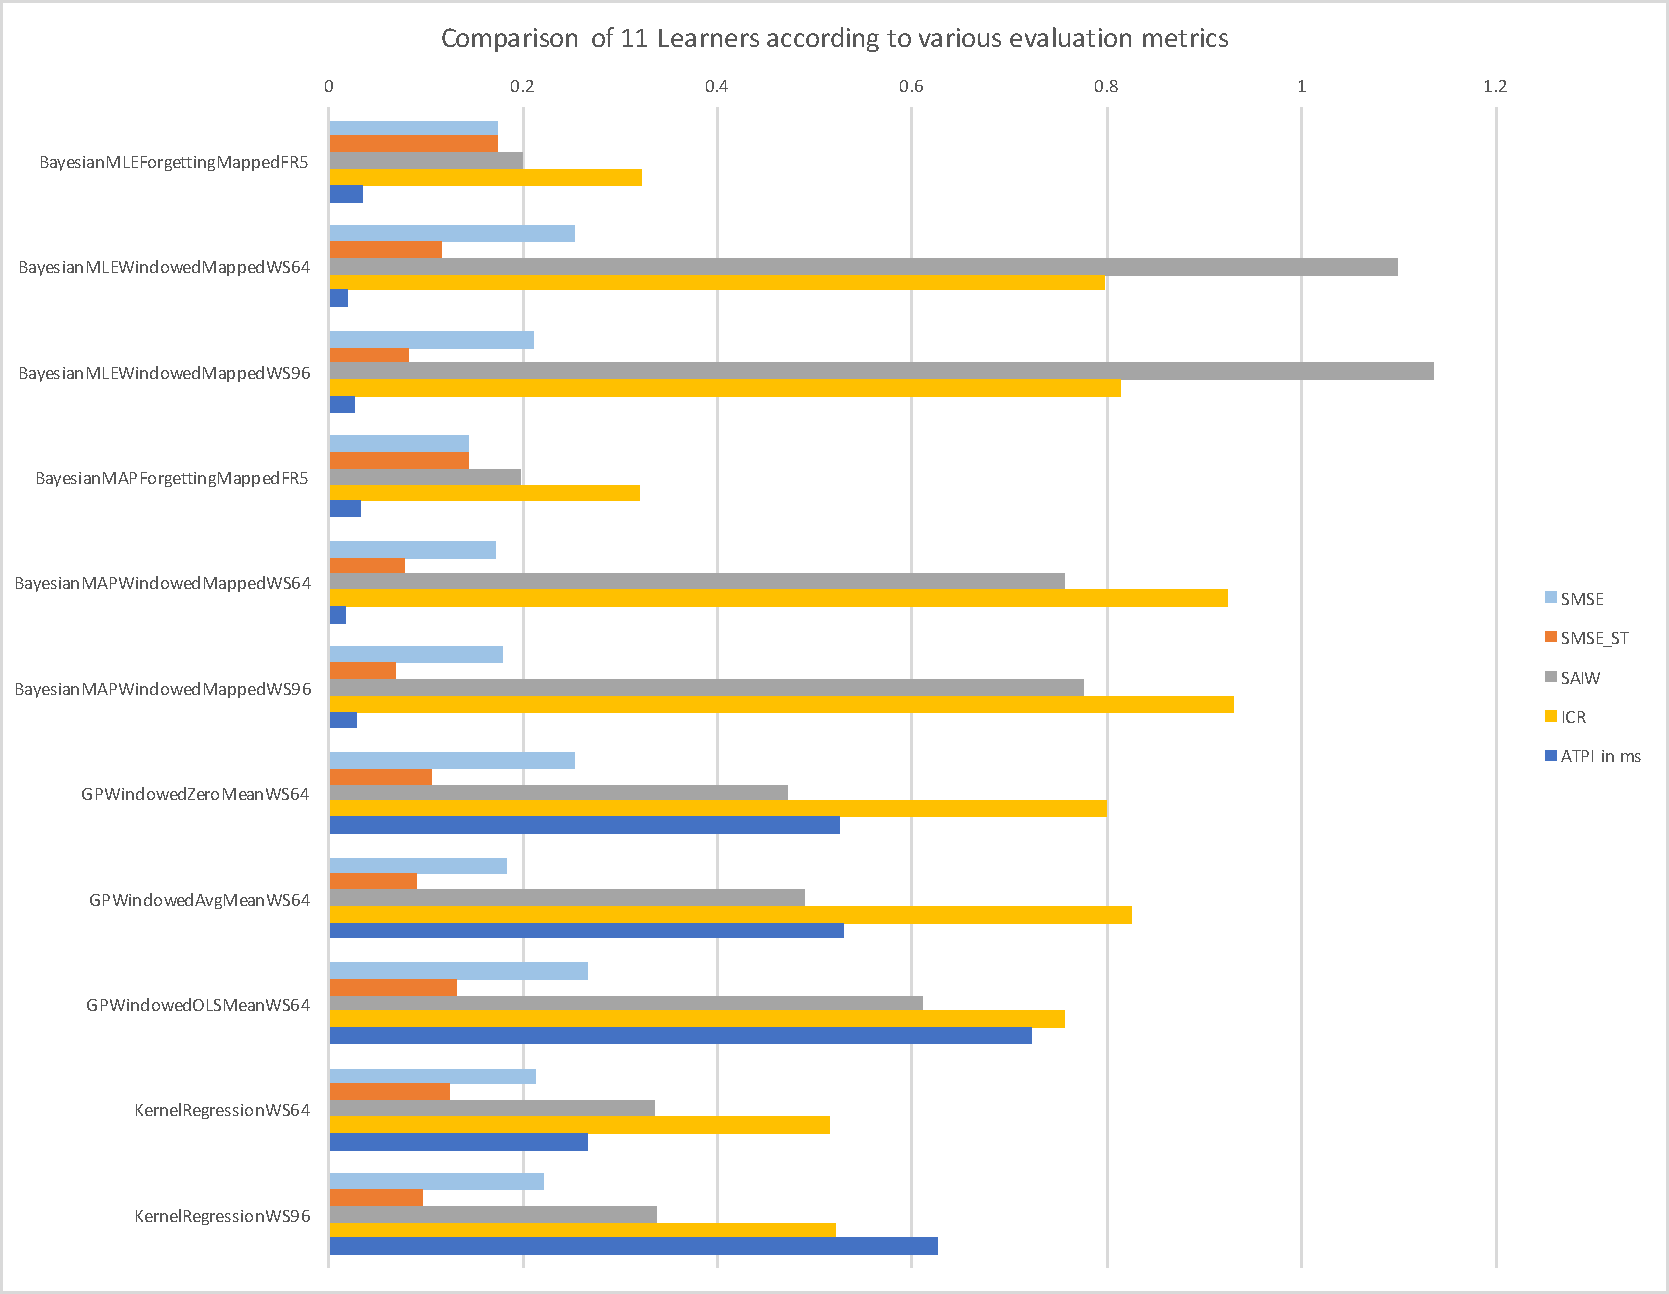
\includegraphics[width=\linewidth]{./Figures/final_11_comparison.pdf}
  \caption{Comparison of \texttt{SMSE}, \texttt{SAIW}, \texttt{ICR} and PIT statistics for 11 different learners whose full codenames are shown on the x- axis. The results are aggregated over the 576 session results.}
  \label{fig:final_11_comparison}
\end{figure}

\begin{figure}[htbp]
  \centering
    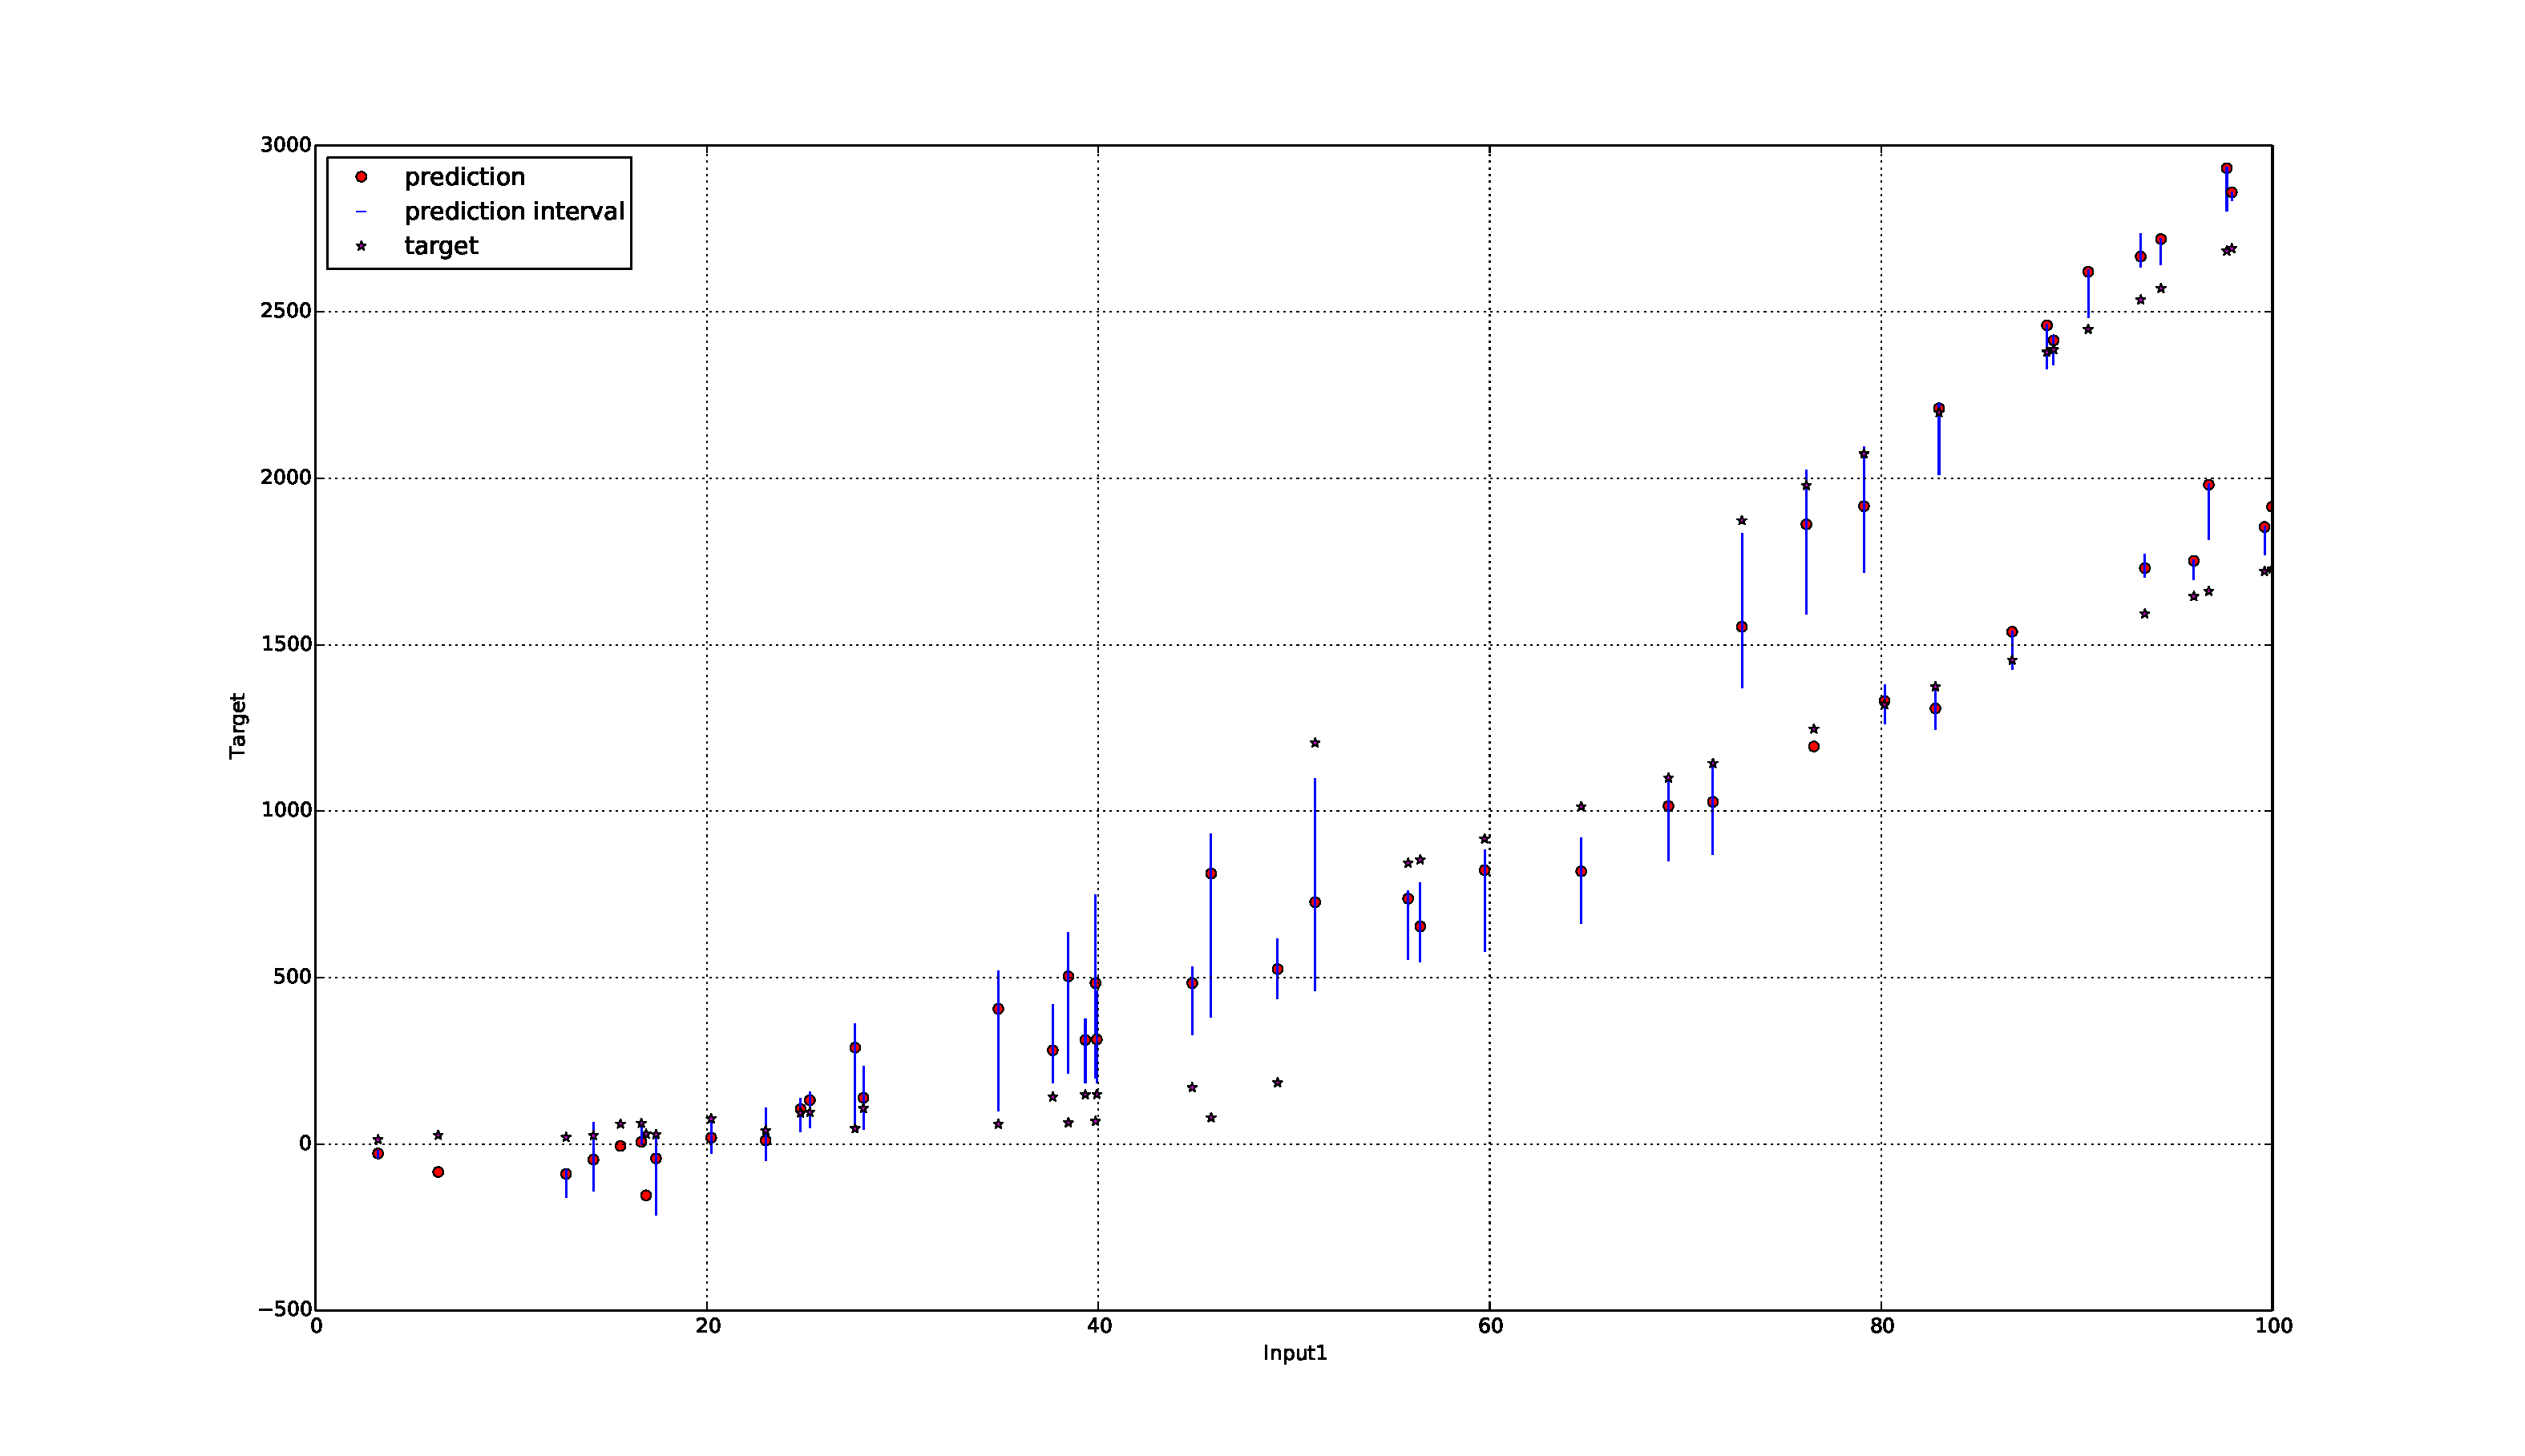
\includegraphics[width=\linewidth]{./Figures/sampled_50_predictions_bmle_mapped_fr5_SYNTH_D_CD_2000_1_100_1_12.pdf}
  \caption{\texttt{BayesianMLEForgettingMapped\_FF0.05} tested on SYNTH\_D\_CD\_2000\_1\_100\_1\_12. 50 sample predictions along with their corresponding targets and prediction intervals are shown}
 \label{fig:sampled_50_predictions_bmle_mapped_fr5_SYNTH_D_CD_2000_1_100_1_12}
\end{figure}

\begin{figure}[htbp]
  \centering
    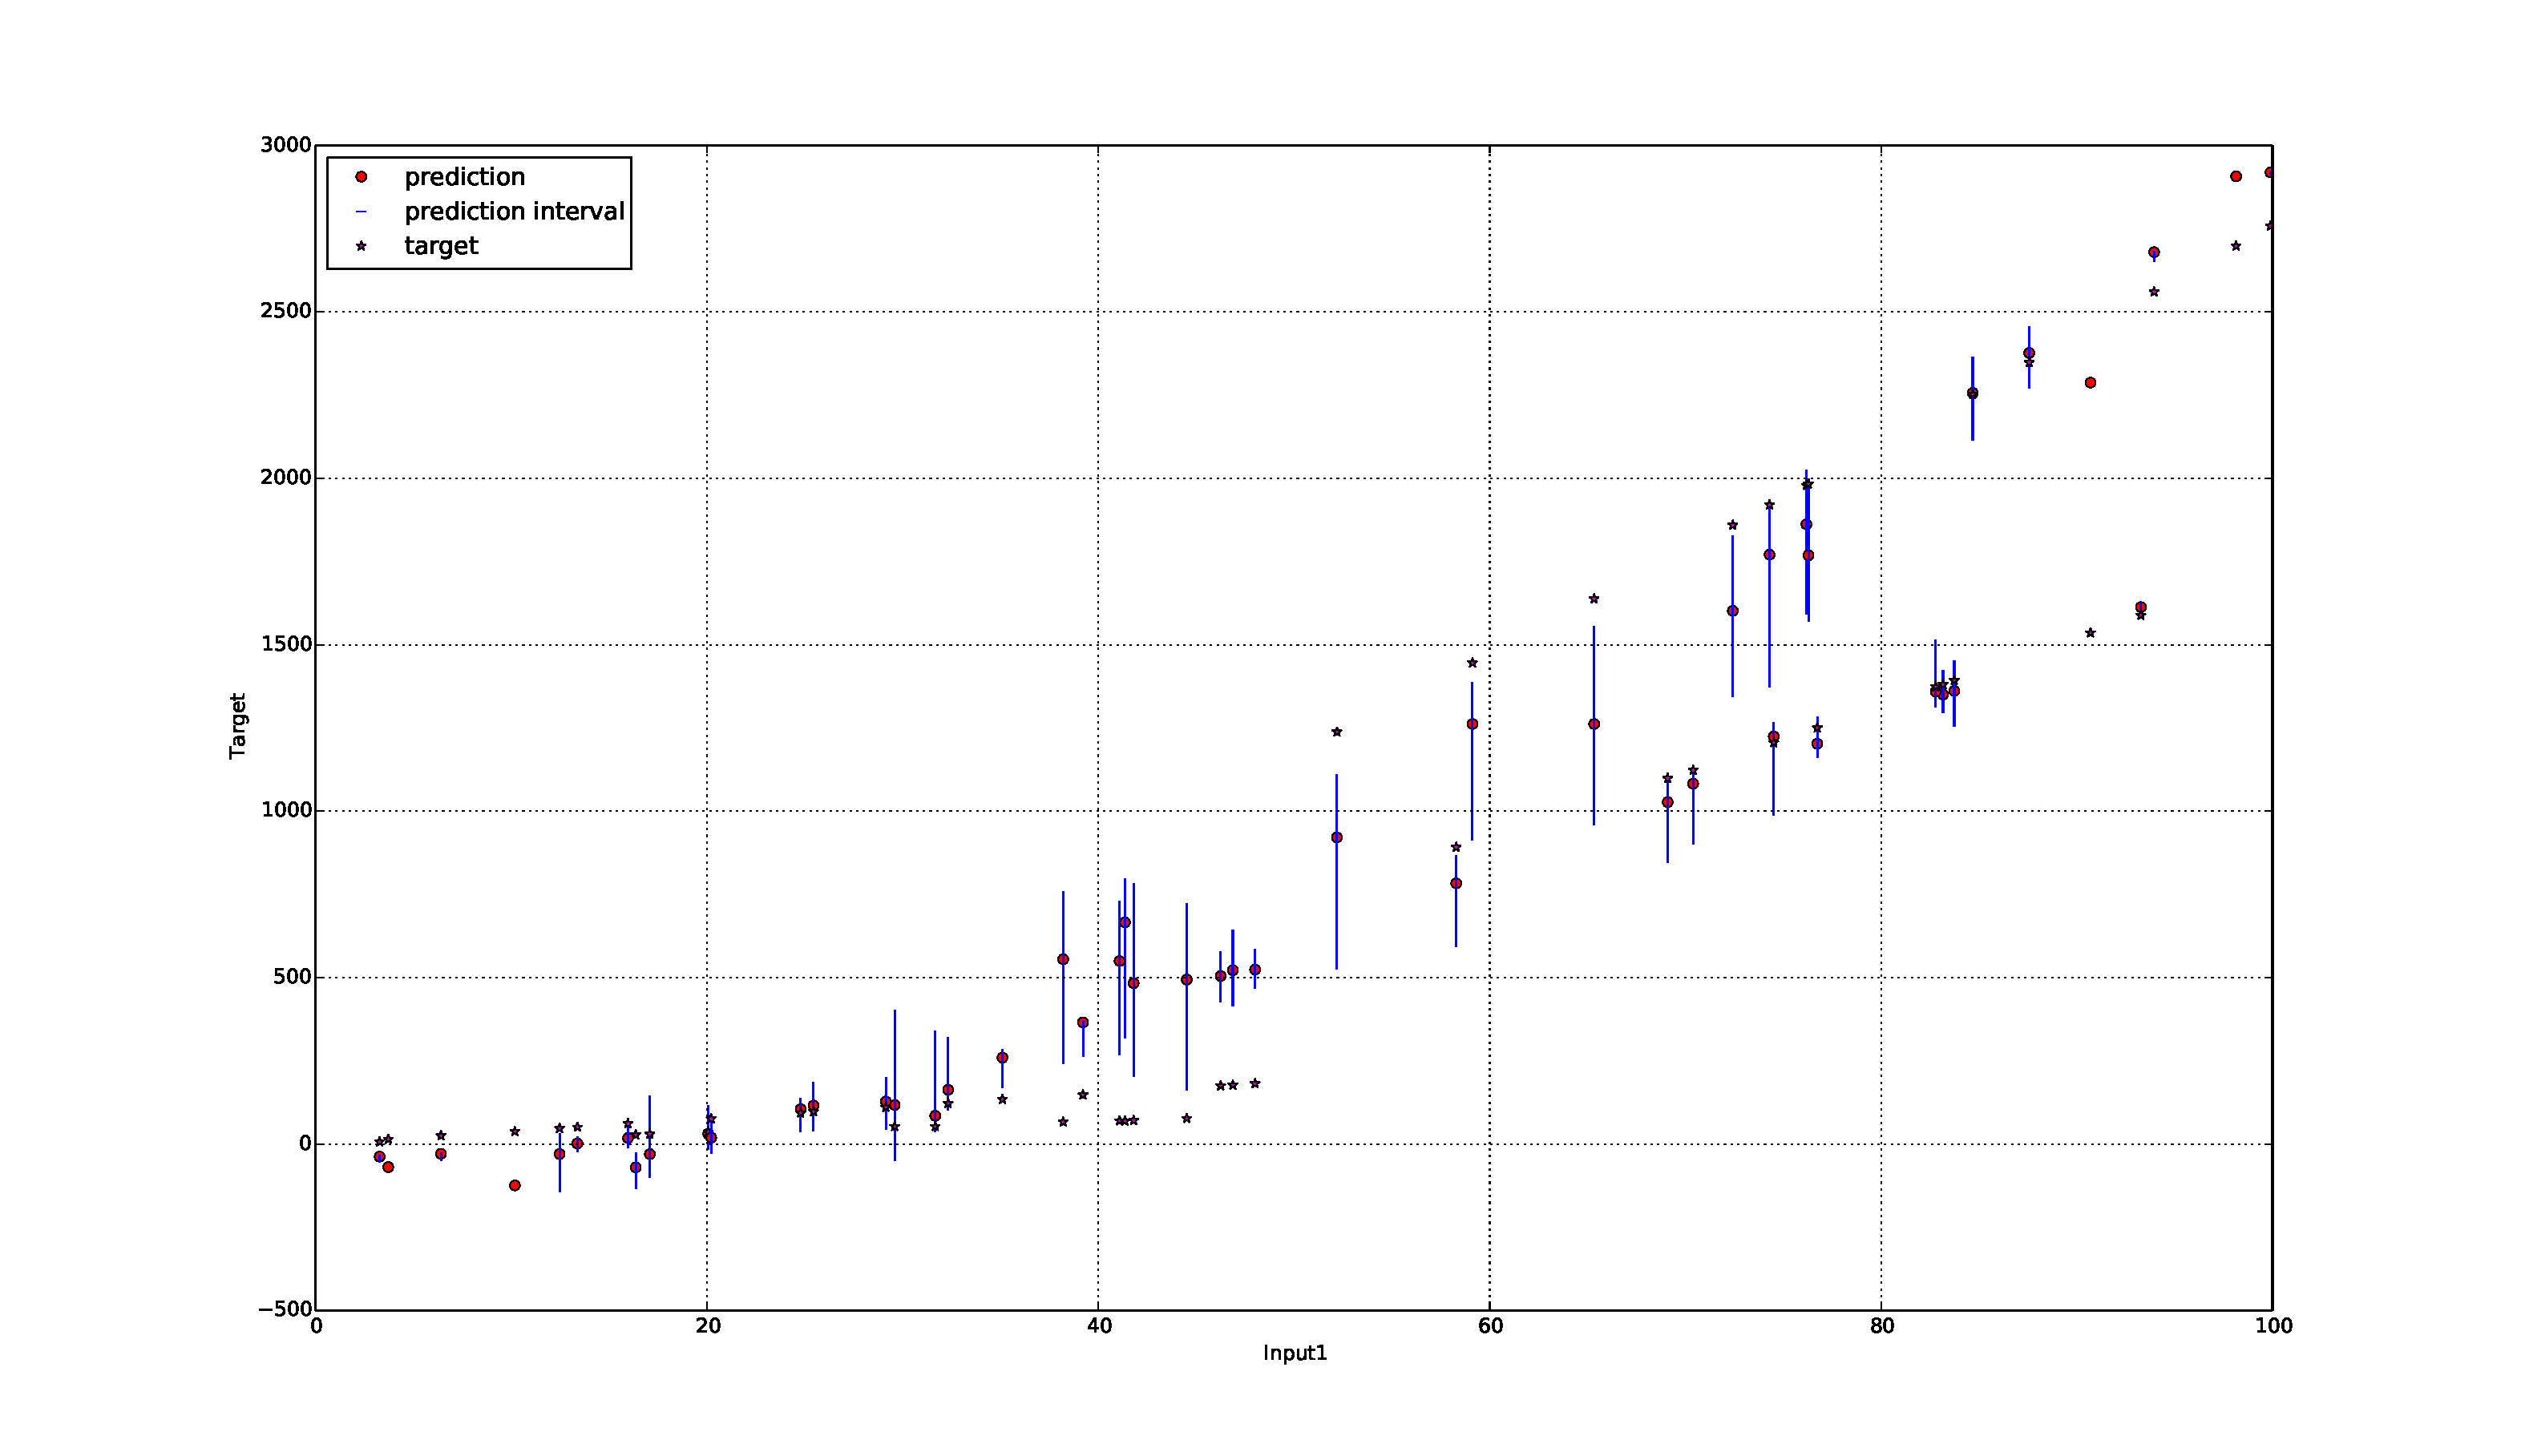
\includegraphics[width=\linewidth]{./Figures/sampled_50_predictions_bmap_mapped_fr5_SYNTH_D_CD_2000_1_100_1_12.pdf}
  \caption{\texttt{BayesianMAPForgettingMapped\_FF0.05} tested on SYNTH\_D\_CD\_2000\_1\_100\_1\_12. 50 sample predictions along with their corresponding targets and prediction intervals are shown}
 \label{fig:sampled_50_predictions_bmap_mapped_fr5_SYNTH_D_CD_2000_1_100_1_12}
\end{figure}

Evidently, forgetting-factor based learners does not provide prediction bounds having good coverage of the target values. Thus, using forgetting-factor based learners for the runtime estimation is not a good idea despite their desirable properties also shared by sliding-windowed learners such as high prediction and update speeds and acceptable accuracy scores.

Other parametric learners apart from the forgetting-based ones also exhibit problems with the prediction bounds they produce. In Figure \ref{fig:final_11_comparison}, it appears that \texttt{SAIW} scores of \texttt{BayesianMLE} algorithms are above 1.0 and the \texttt{SAIW} scores of \texttt{BayesianMAP} are close to $0.8$. These \texttt{SAIW} scores indicate that the average gap between the upper and the lower prediction bounds is very high. For reference, one can imagine having the \texttt{SAIW} score if $1.0$ being equivalent of producing lower and upper prediction bounds that are as far as the magnitude of the target mean apart from each other. In order to visualize how high that is, randomly chosen $25$ data points occurred on a simulated stream which each of the sliding-windowed parametric algorithms from the list \ref{final_11} are tested along with the target, prediction and prediction bounds of them are visualized in \ref{fig:sampled_25_predictions_bmle_mapped_ws64_SYNTH_D_NCD_2000_2_50_3_12},
\ref{fig:sampled_25_predictions_bmle_mapped_ws96_SYNTH_D_NCD_2000_2_50_3_12},
\ref{fig:sampled_25_predictions_bmap_mapped_ws64_SYNTH_D_NCD_2000_2_50_3_12},
and \ref{fig:sampled_25_predictions_bmap_mapped_ws96_SYNTH_D_NCD_2000_2_50_3_12}.
Some of the prediction intervals shown with the blue lines in the graphs are too big that lower bound of some of them are even negative which do not make sense for runtime predictions.

\begin{figure}[htbp]
  \centering
    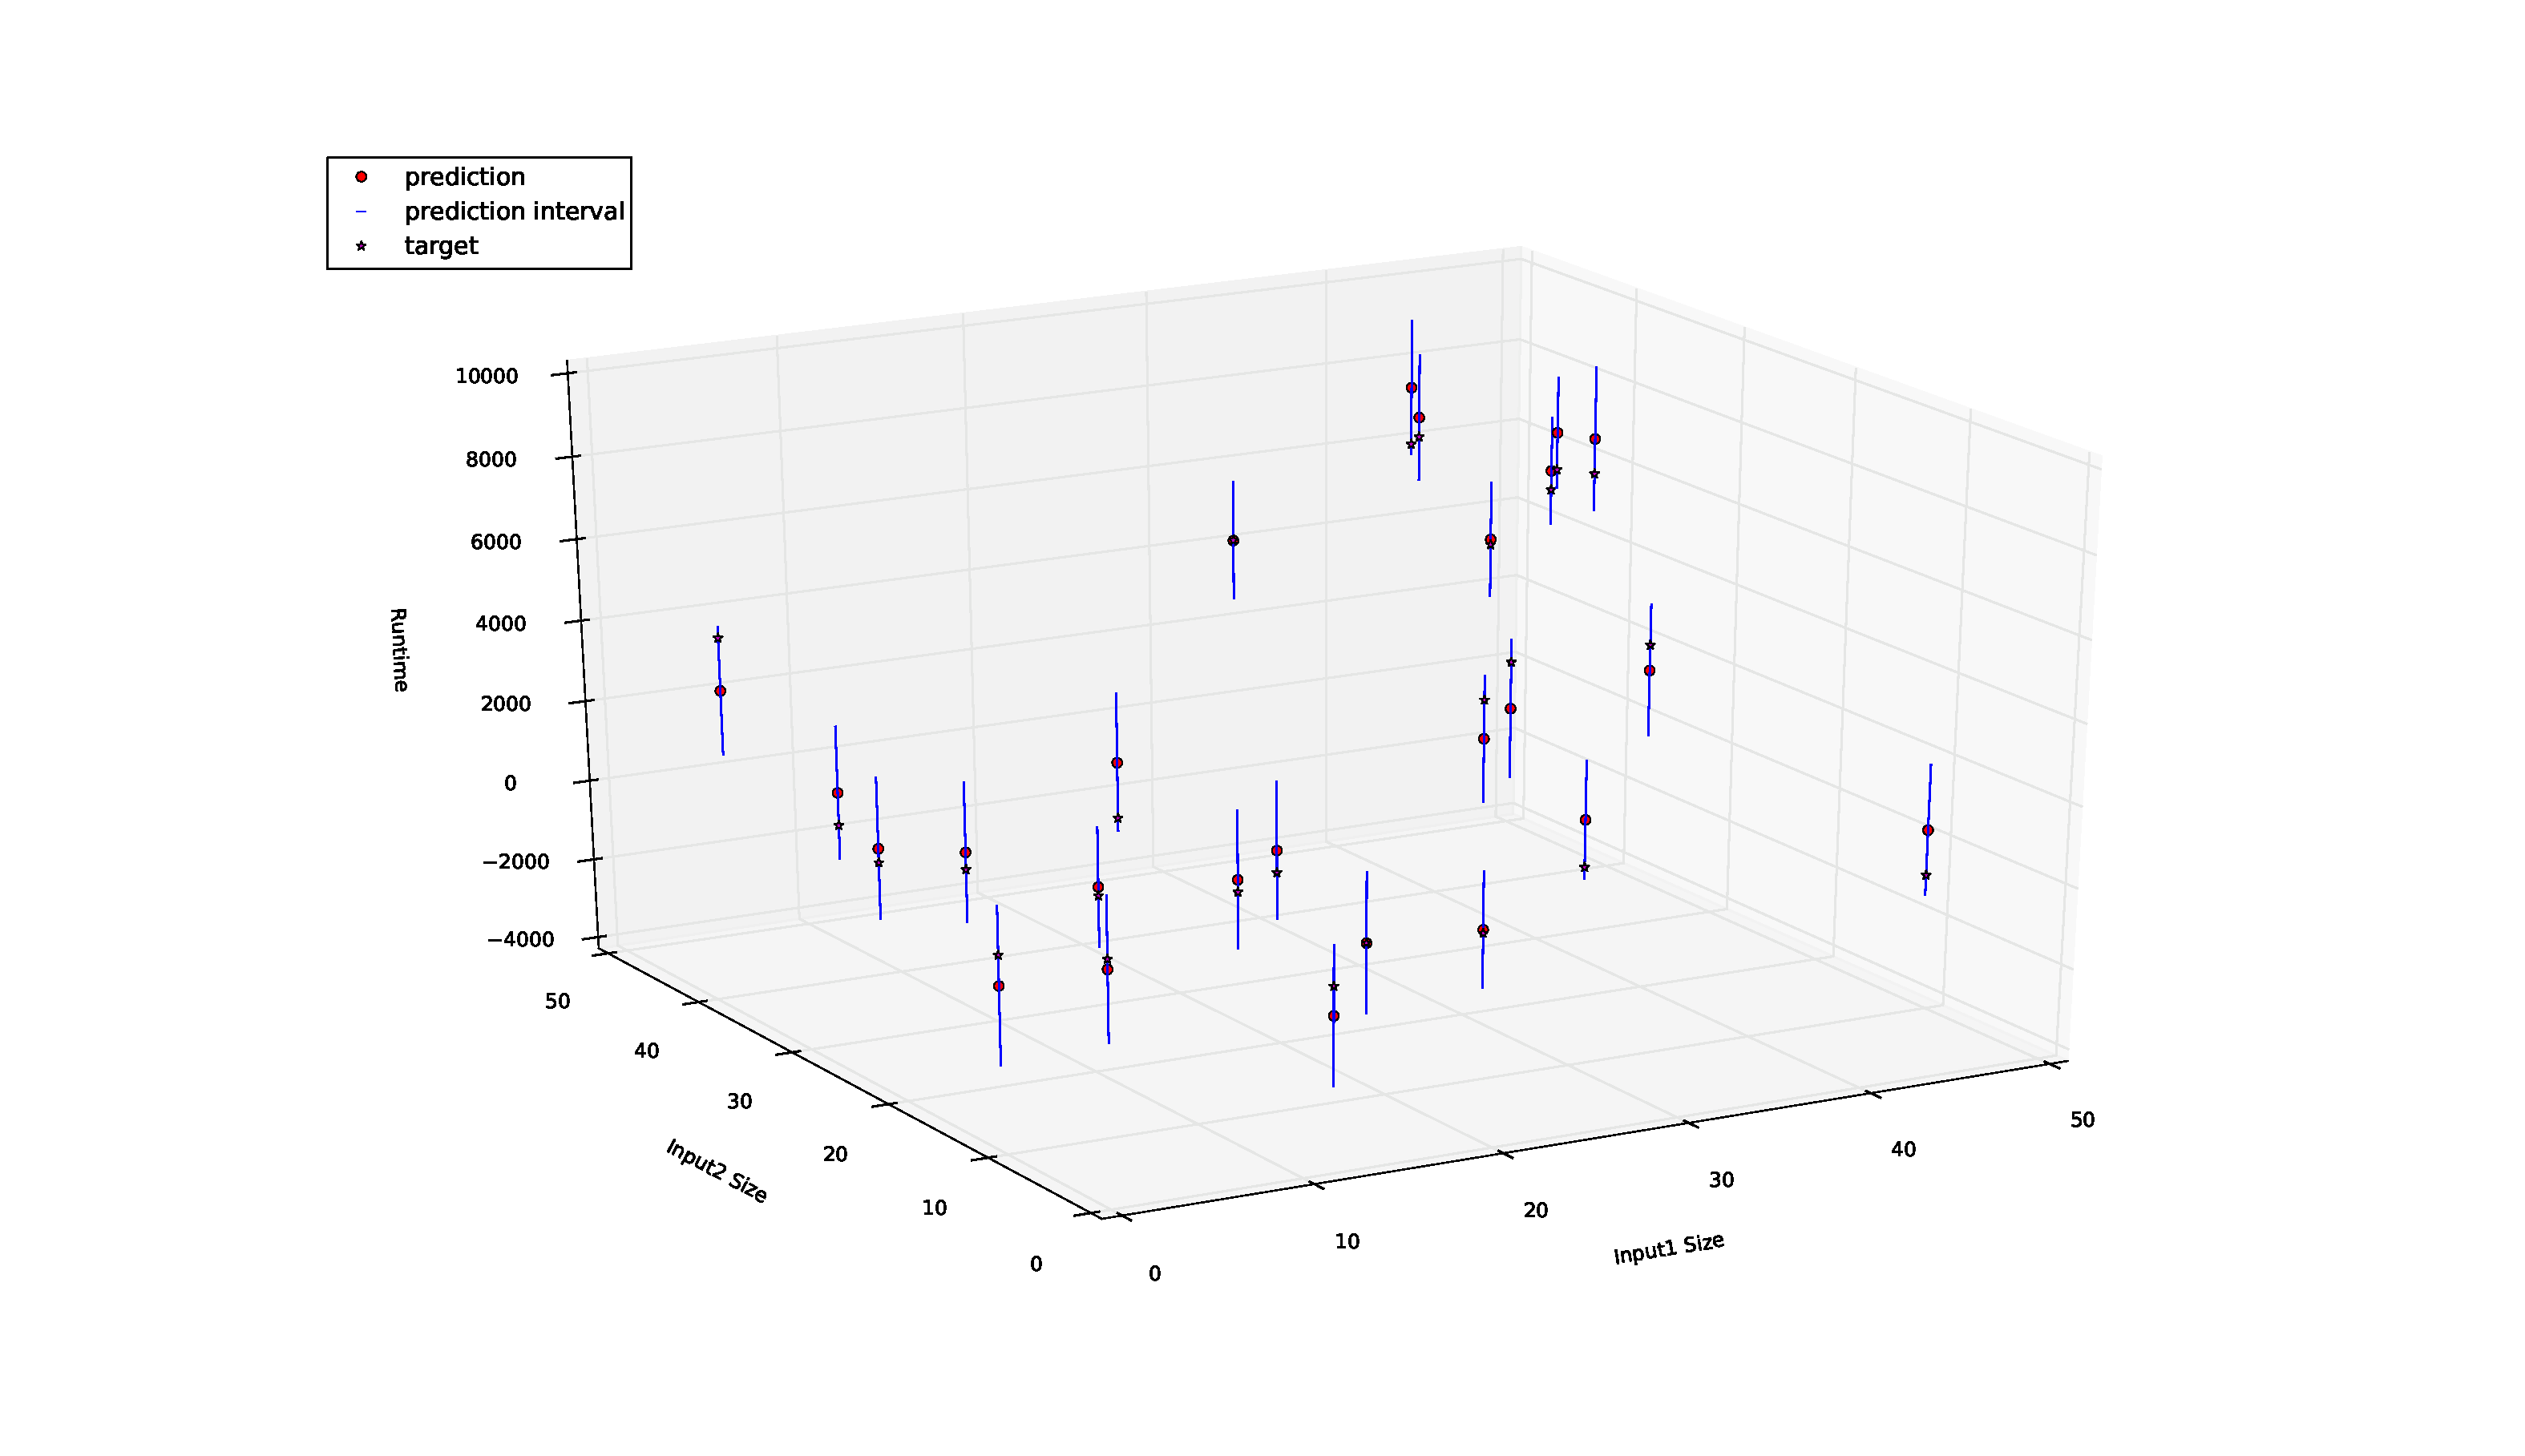
\includegraphics[width=\linewidth]{./Figures/sampled_25_predictions_bmle_mapped_ws64_SYNTH_D_NCD_2000_2_50_3_12.pdf}
  \caption{\texttt{BayesianMLEWindowedMapped\_WS64} tested on \texttt{SYNTH\_N\_NCD\_2000\_2\_50\_3\_12}. 25 sample predictions along with their corresponding targets and prediction intervals are shown}
 \label{fig:sampled_25_predictions_bmle_mapped_ws64_SYNTH_D_NCD_2000_2_50_3_12}
\end{figure}

\begin{figure}[htbp]
  \centering
    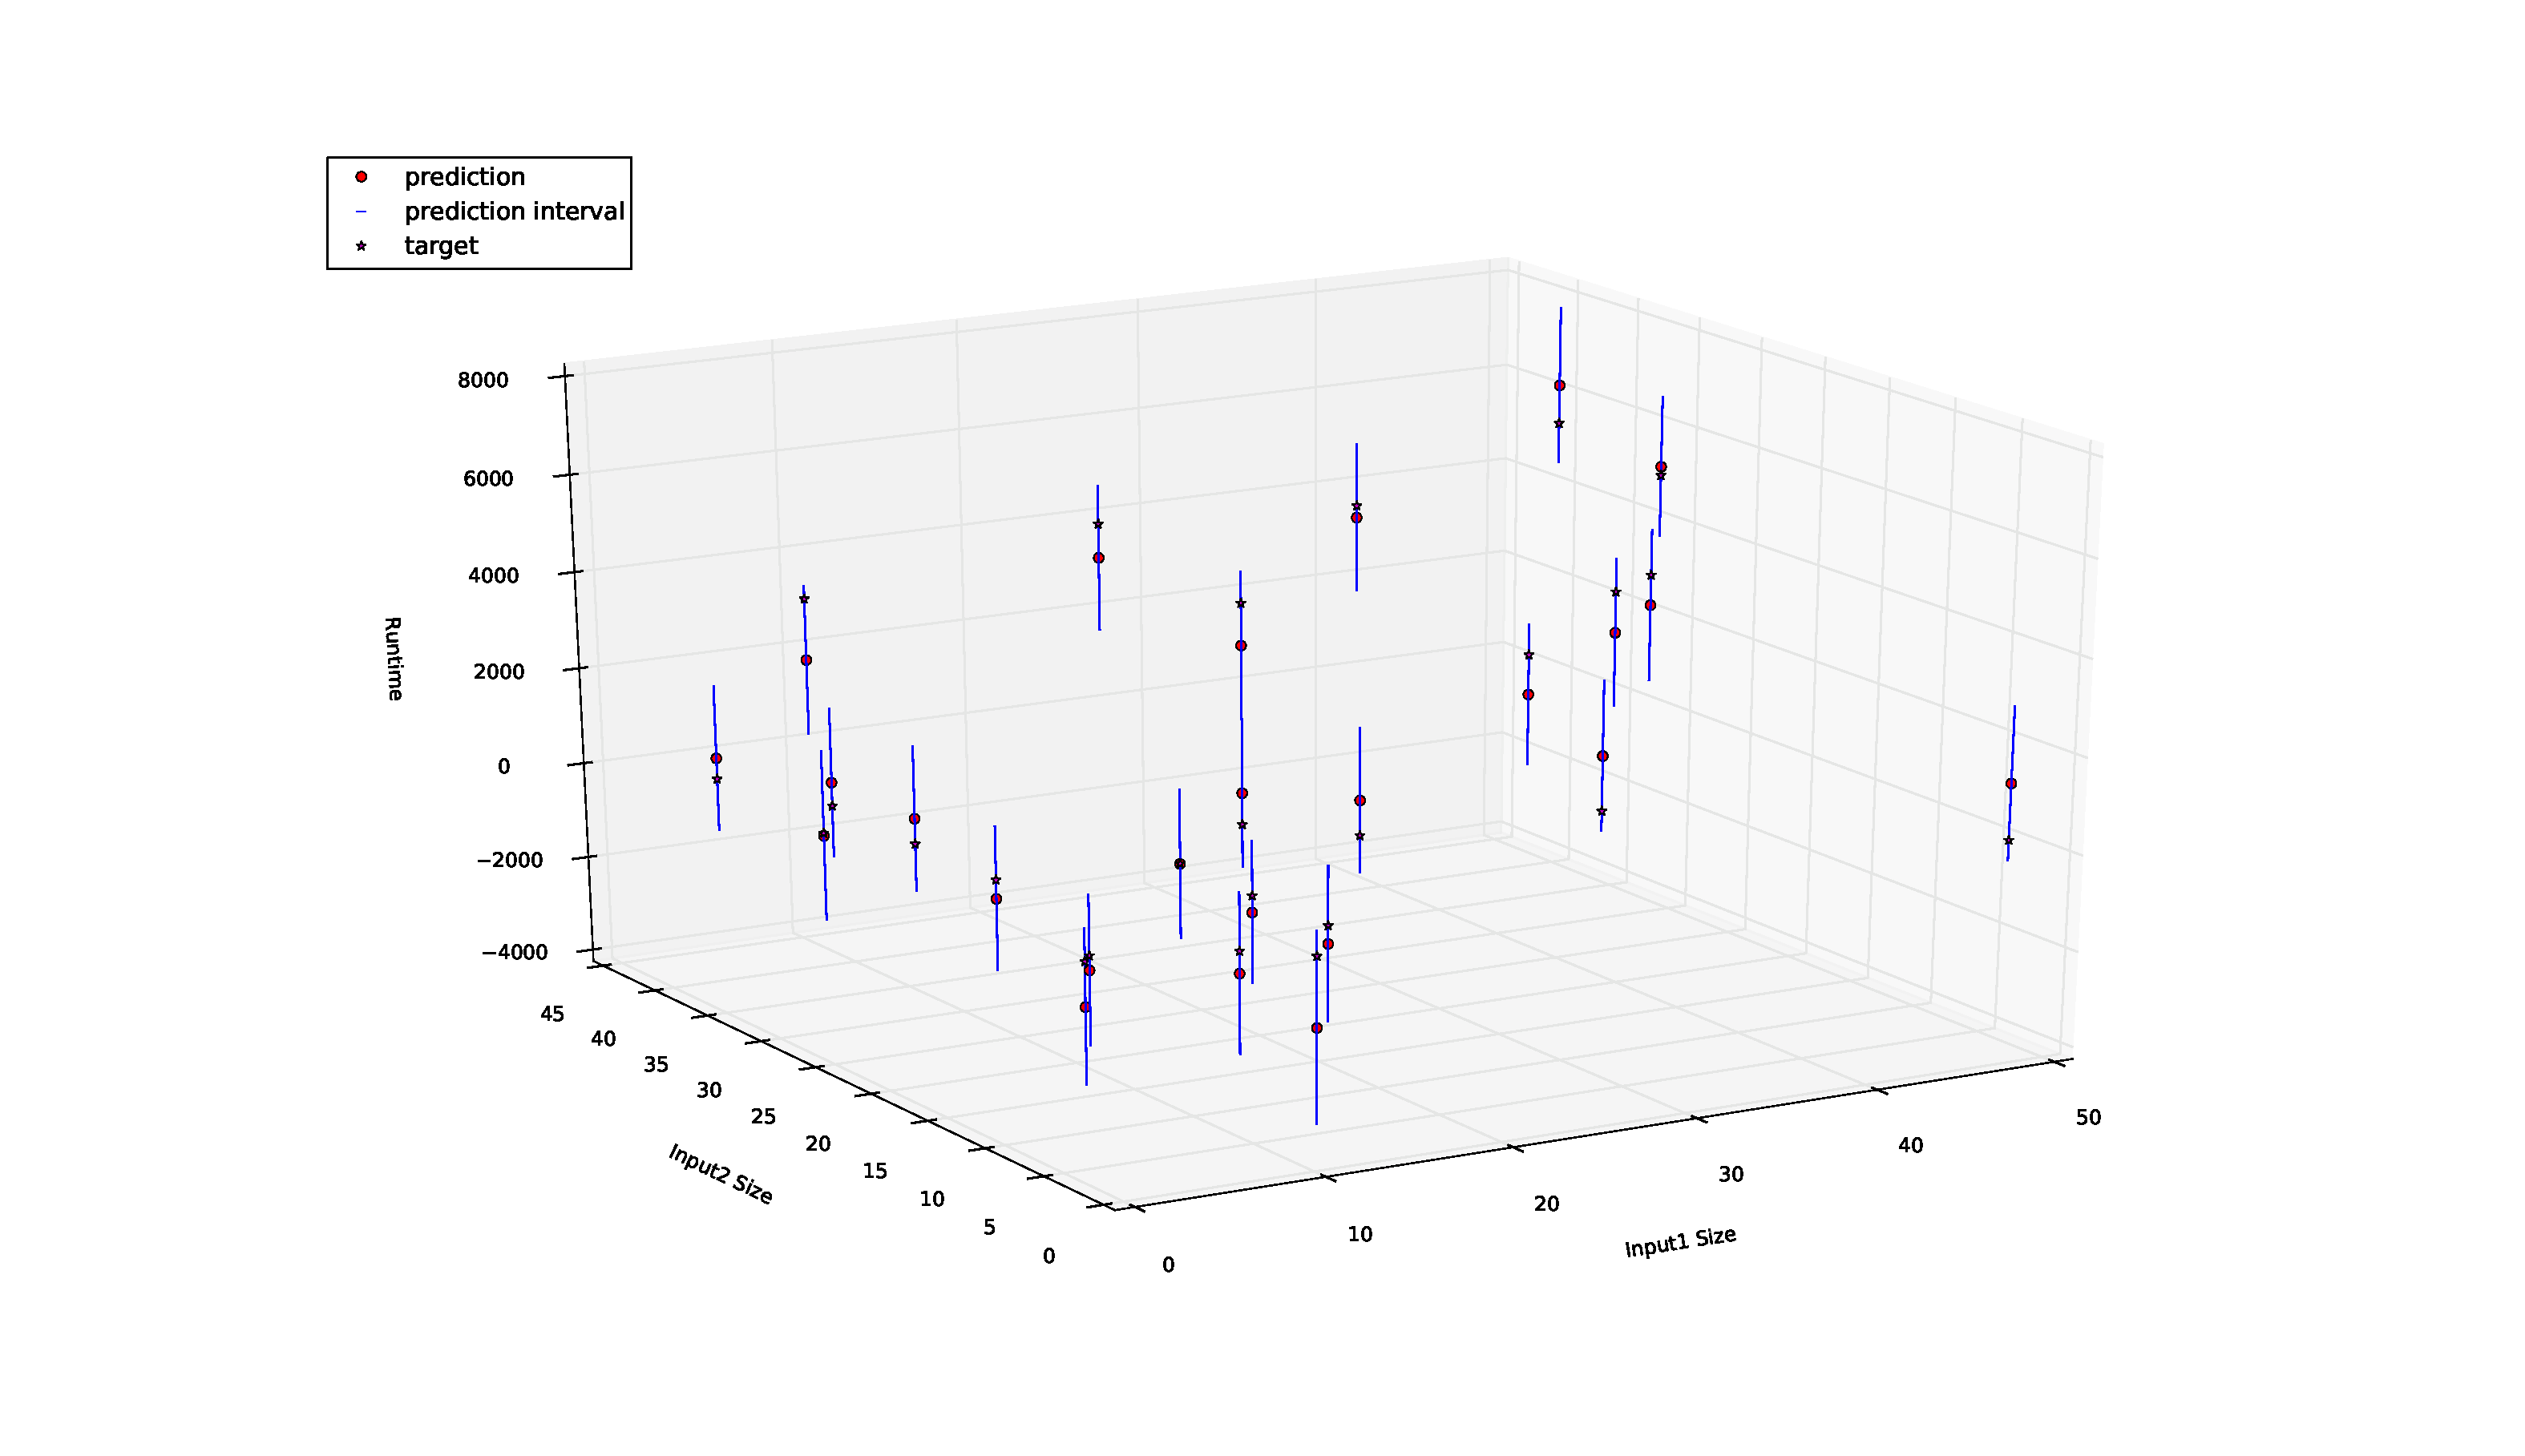
\includegraphics[width=\linewidth]{./Figures/sampled_25_predictions_bmle_mapped_ws96_SYNTH_D_NCD_2000_2_50_3_12.pdf}
  \caption{\texttt{BayesianMLEWindowedMapped\_WS96} tested on \texttt{SYNTH\_N\_NCD\_2000\_2\_50\_3\_12}. 25 sample predictions along with their corresponding targets and prediction intervals are shown}
 \label{fig:sampled_25_predictions_bmle_mapped_ws96_SYNTH_D_NCD_2000_2_50_3_12}
\end{figure}

\begin{figure}[htbp]
  \centering
    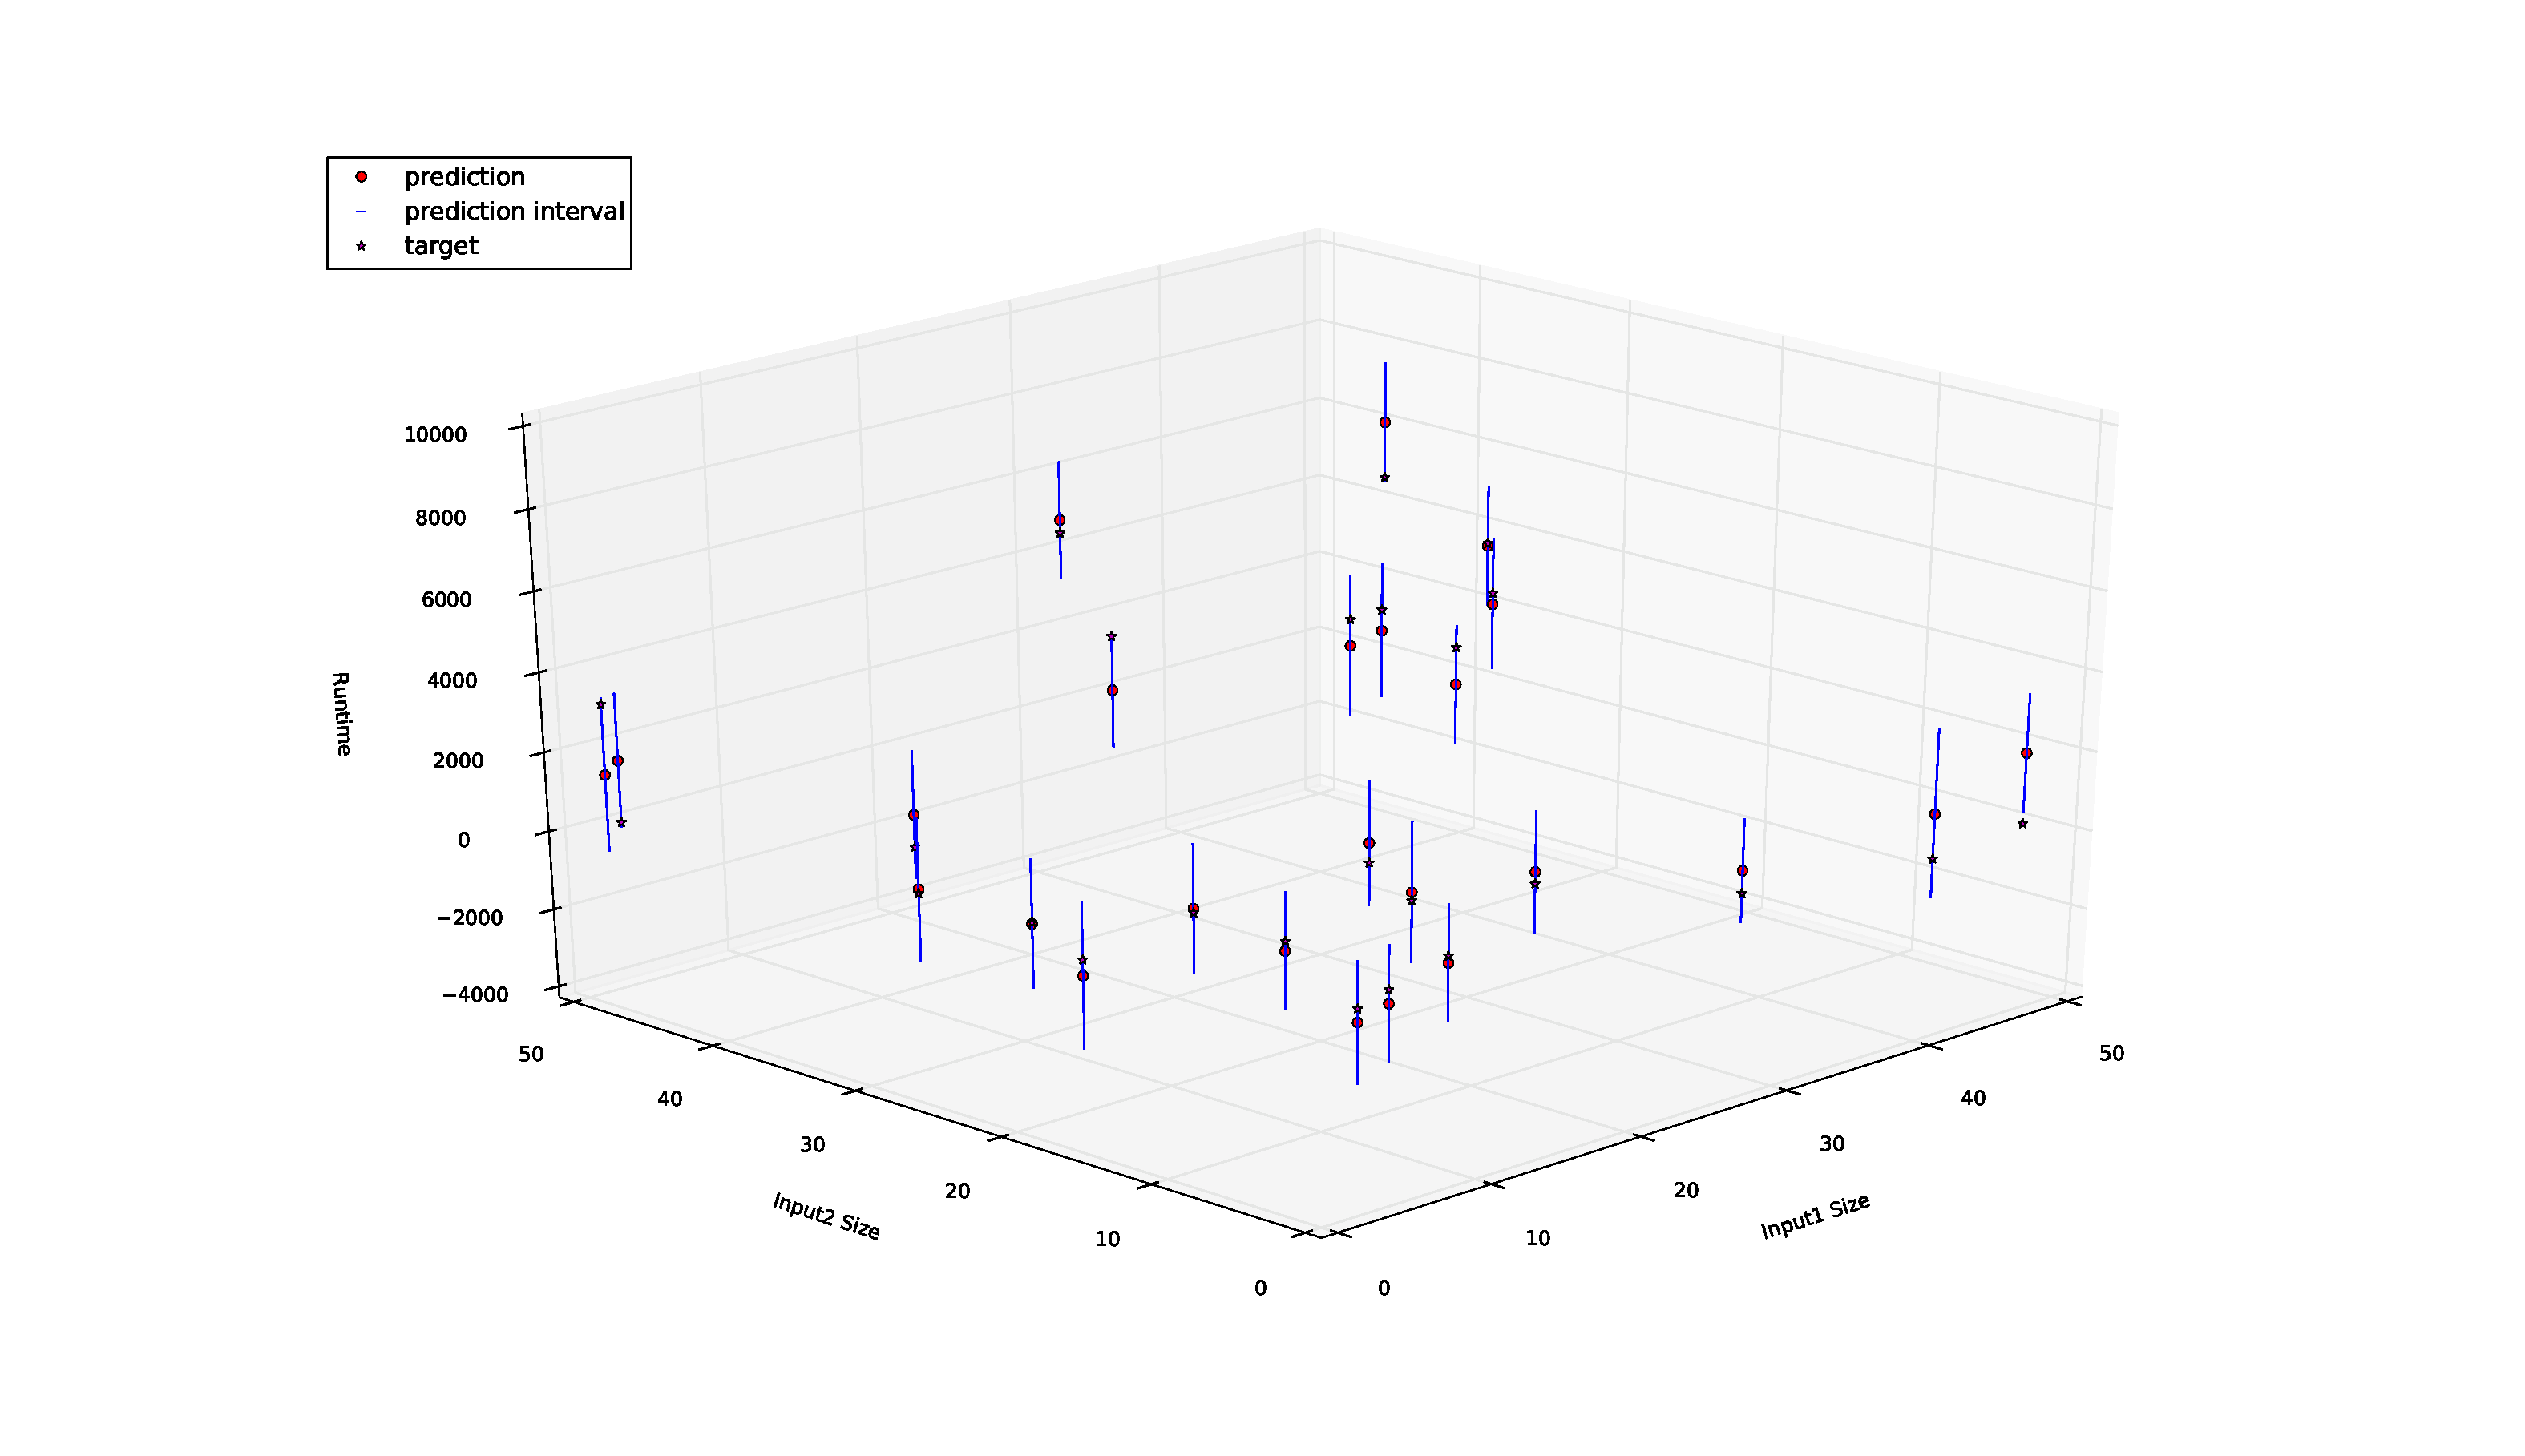
\includegraphics[width=\linewidth]{./Figures/sampled_25_predictions_bmap_mapped_ws64_SYNTH_D_NCD_2000_2_50_3_12.pdf}
  \caption{\texttt{BayesianMAPWindowedMapped\_WS64} tested on \texttt{SYNTH\_N\_NCD\_2000\_2\_50\_3\_12}. 25 sample predictions along with their corresponding targets and prediction intervals are shown}
 \label{fig:sampled_25_predictions_bmap_mapped_ws64_SYNTH_D_NCD_2000_2_50_3_12}
\end{figure}

\begin{figure}[htbp]
  \centering
    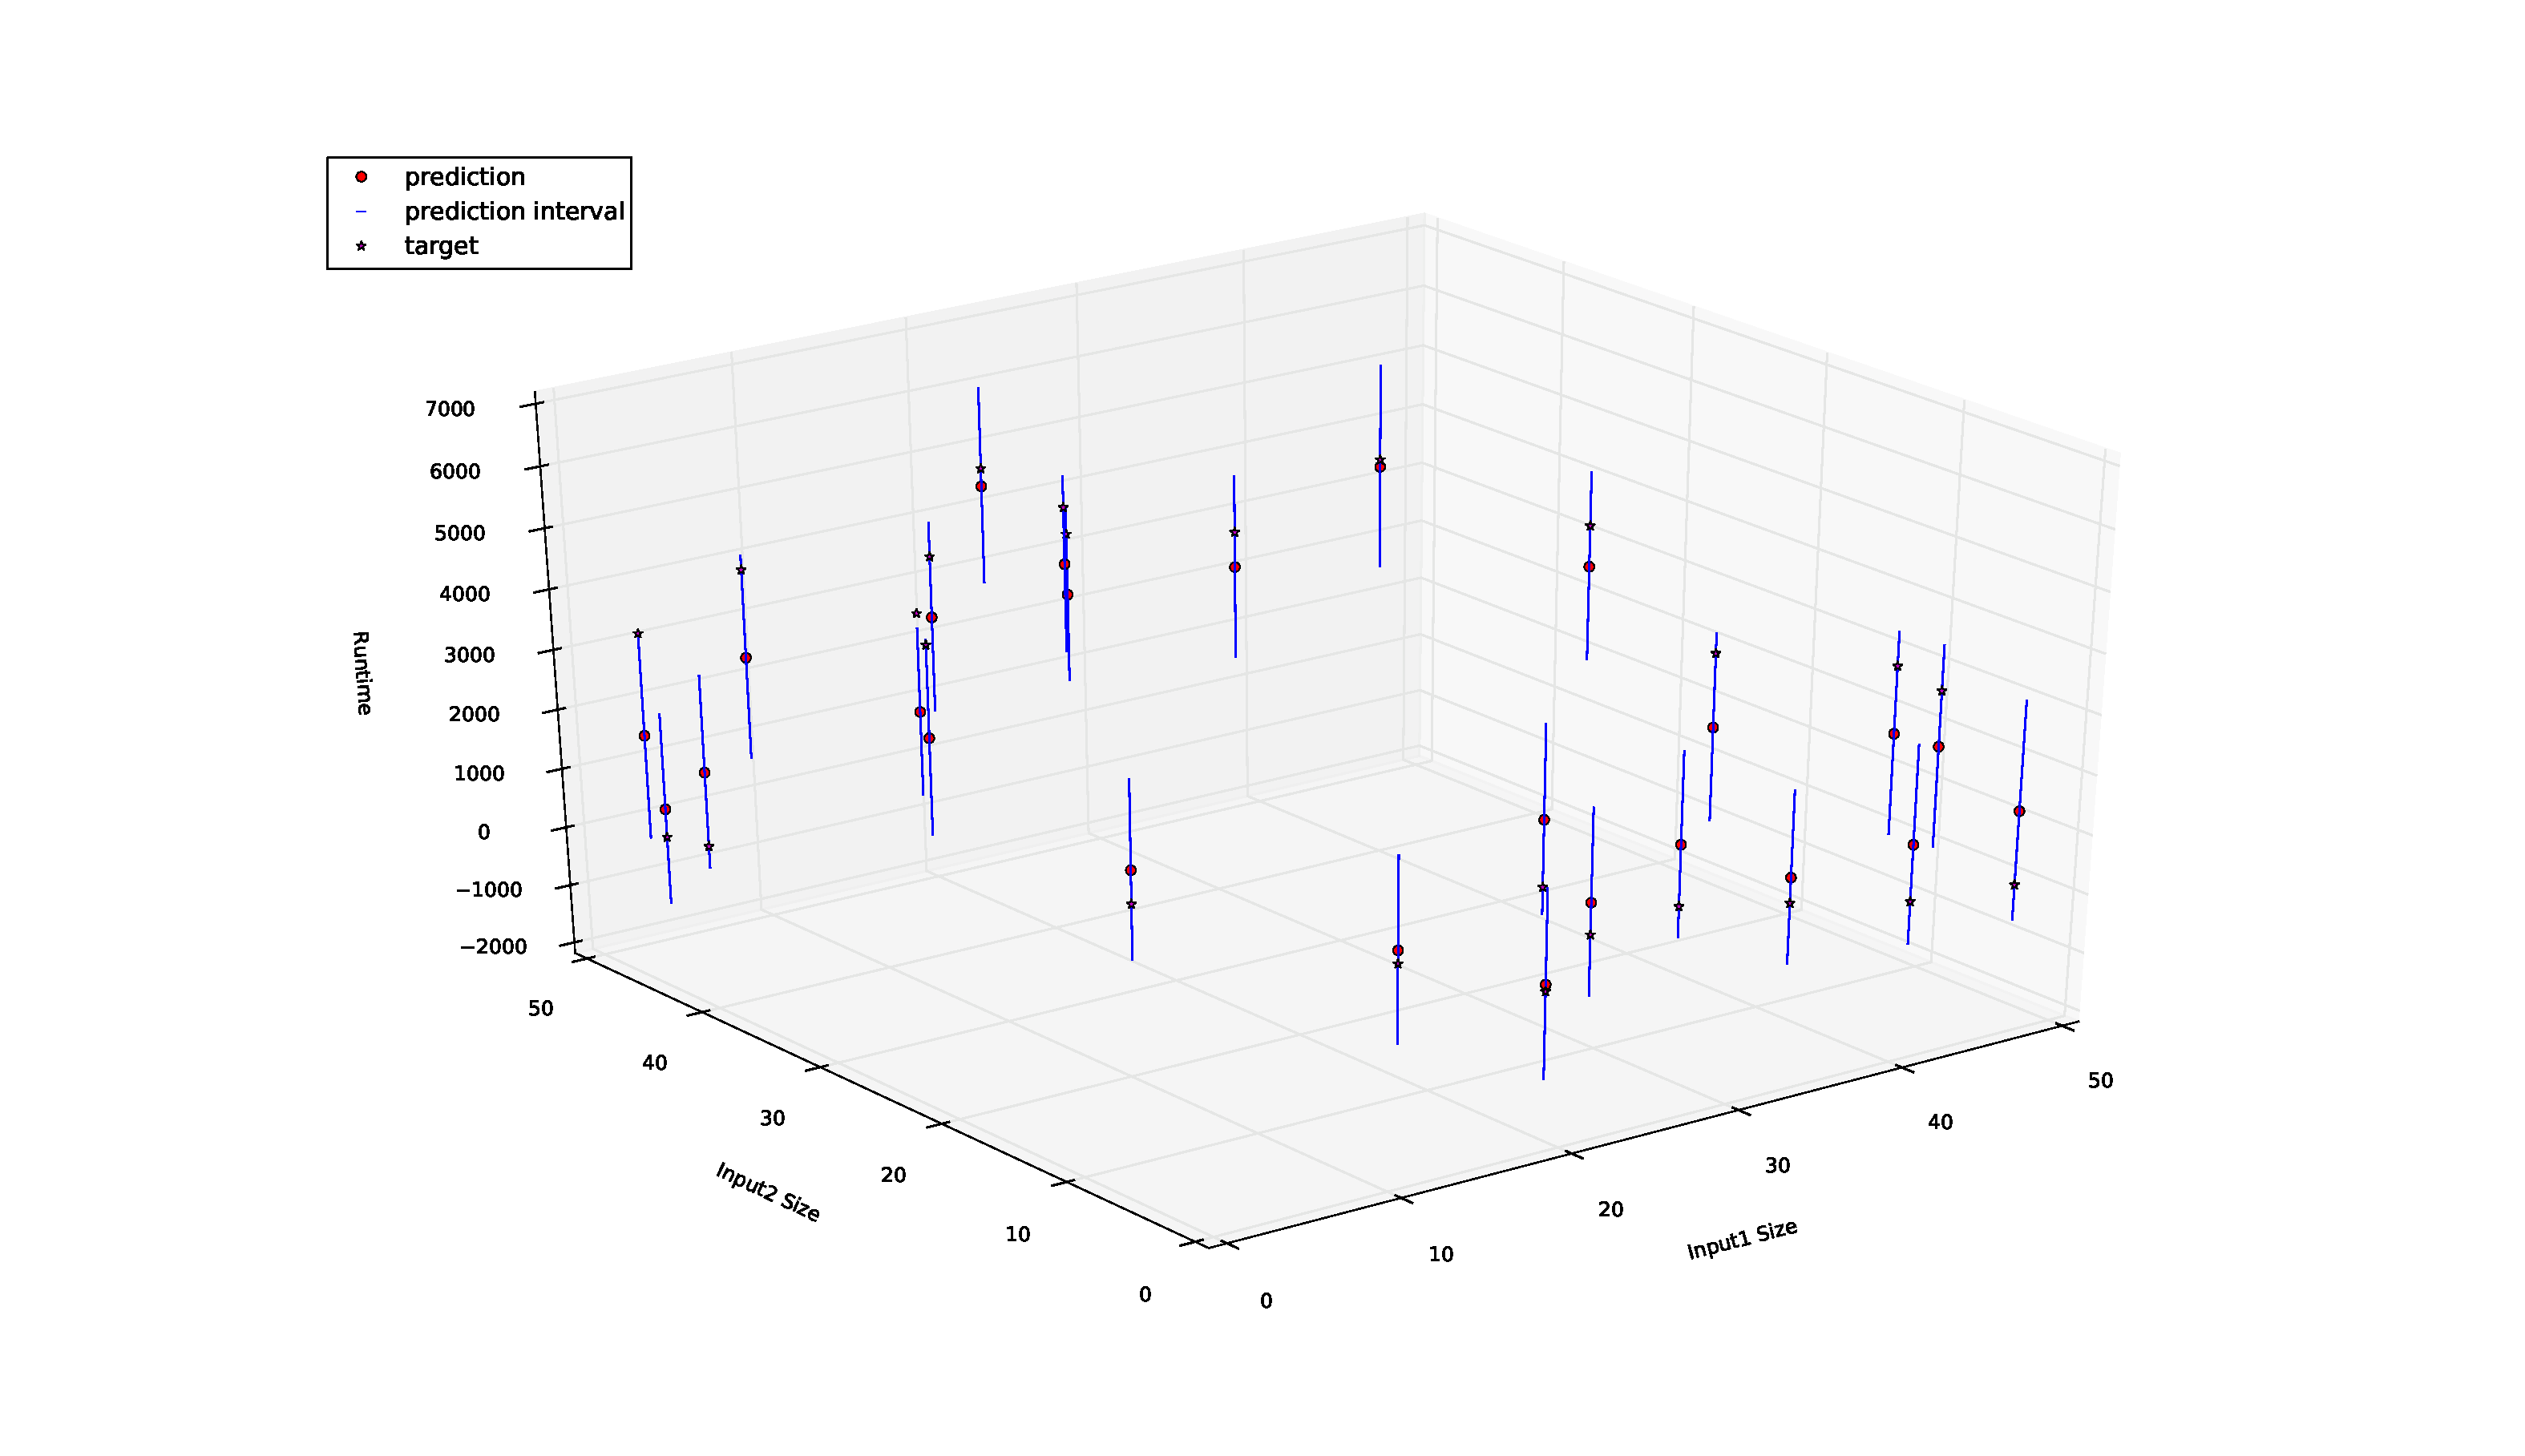
\includegraphics[width=\linewidth]{./Figures/sampled_25_predictions_bmap_mapped_ws96_SYNTH_D_NCD_2000_2_50_3_12.pdf}
  \caption{\texttt{BayesianMAPWindowedMapped\_WS96} tested on \texttt{SYNTH\_N\_NCD\_2000\_2\_50\_3\_12}. 25 sample predictions along with their corresponding targets and prediction intervals are shown}
 \label{fig:sampled_25_predictions_bmap_mapped_ws96_SYNTH_D_NCD_2000_2_50_3_12}
\end{figure}
 
For the sake of explaining why the theoretically sound prediction interval estimation method (unlike the one used by the forgetting-factor based learners) employed by the sliding-windowed \texttt{BayesianMAP} and \texttt{BayesianMLE} variants did not work as expected, the experiment data is analyzed from the streams simulated by the data which is generated by a function with discontinuity and without discontinuity separately. This is because, the only data quality that may have caused a parametric regression algorithm fail to make accurate predictions with tight prediction bounds is discontinuity of the function that is used to generate the data. To this end, a graph with showing only \texttt{ICR} and \texttt{SAIW} scores of the sliding window algorithms considered in \ref{final_11} on the streams of different natures in terms of the continuity of the data generation function used for the generation of the data set which they are simulated from is prepared.

\begin{figure}[htbp]
  \centering
    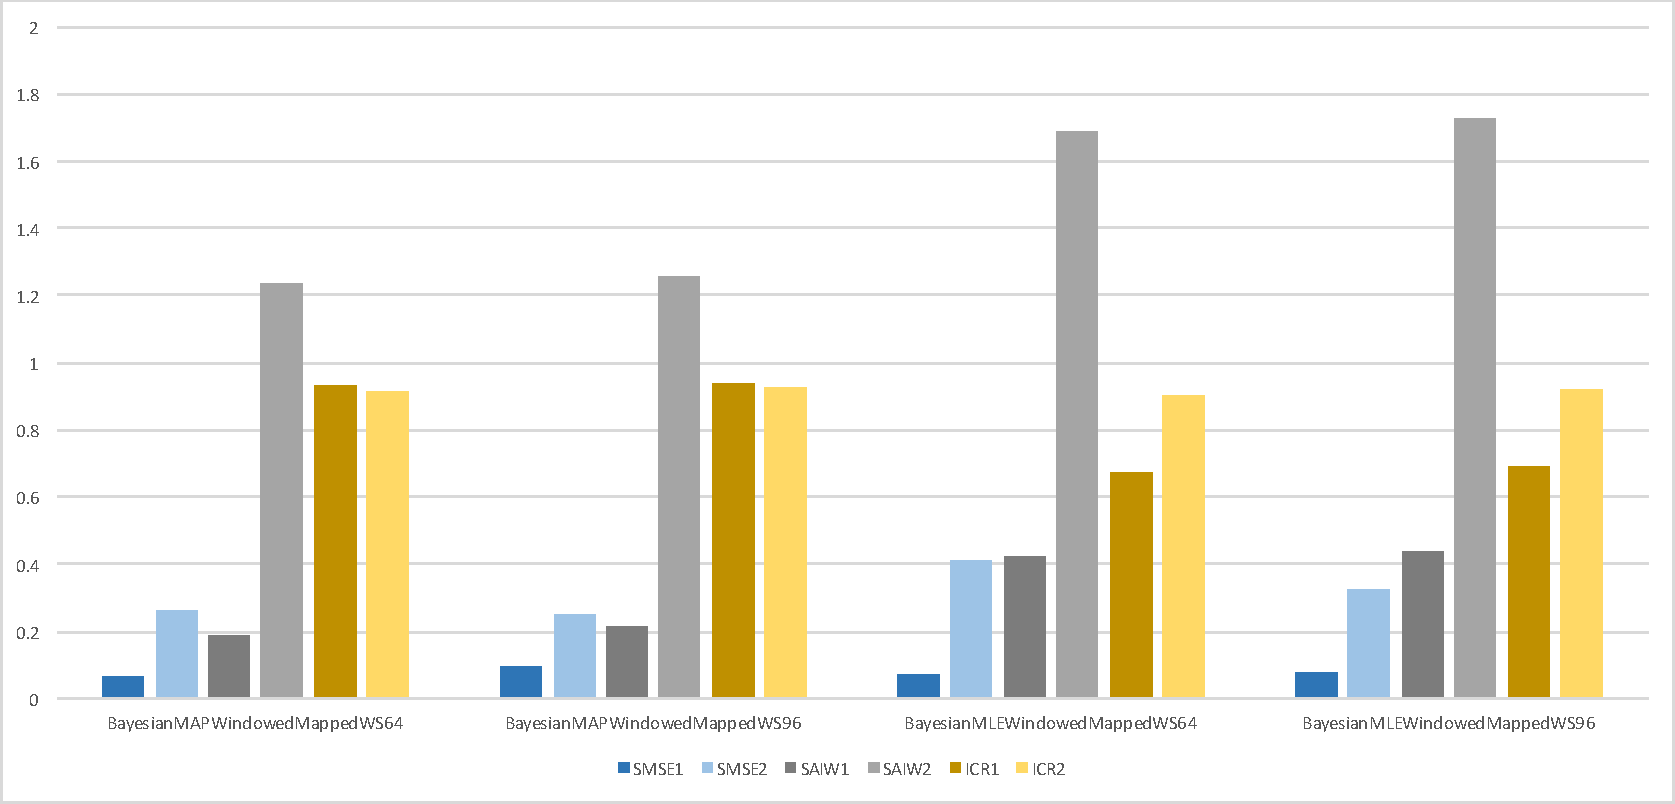
\includegraphics[width=\linewidth]{./Figures/disc_nondisc_bmap_bmap_mapped_ws64_ws96.pdf}
  \caption{A comparison of \texttt{SMSE}, \texttt{SAIW} and \texttt{ICR} metrics for 4 different learners whose full codenames are shown on the x- axis on the streams simulated of different nature in terms of the continuity of the function that generated the data set which they are simulated from. The values are obtained through aggregation of session results of 276 stream simulations for each class}
  \label{fig:disc_nondisc_bmap_bmap_mapped_ws64_ws96}
\end{figure}

In \ref{fig:disc_nondisc_bmap_bmap_mapped_ws64_ws96}, the statistics represented by darker colors (and also denoted by a name ending with 1 in the legend) are obtained from the tests containing data from continuous functions whereas the light ones (in the legend, having names ending with 2) are obtained from the test data generated by discontinuous functions. Looking only at the difference between \texttt{SMSE}1 and \texttt{SMSE}2 values makes is clear the data from the discontinuous functions was the culprit. This is a clear manifestation of \textit{underfitting} explained in Chapter \ref{Chapter2}. Parametric models fail when the data they learn from generated from a function that belongs to a different class than the one assumed by the parametric model. And due to this failure causing large errors for data points, prediction interval estimation method based on the errors accumulated produces very large prediction intervals making \texttt{SAIW} to jump to very high values from dark blue columns to light blue ones in the graph. 

Since the growth of the runtime of the database operators usually change characteristics as the inputs growth as pointed out in Chapter \ref{Chapter3}, synthetic data generated to mock this situation is important. This is why, parametric models that fails to provide prediction bounds of good quality are found unsuitable for runtime estimation problem. 

In Figure \ref{fig:final_11_comparison}, the bottom $2$ bars indicate that \texttt{KernelRegression} learners do not produce prediction bounds that provide high target variable coverage just like forgetting-based parametric learners. In order to visualize the problem with the prediction bounds that \texttt{KernelRegression} learners have, prediction bounds they provided along with the predictions and targets for randomly chosen $50$ data points from a test stream is displayed in \ref{fig:sampled_50_predictions_kreg_ws64_SYNTH_D_CD_2000_1_50_3_23} and \ref{fig:sampled_50_predictions_kreg_ws96_SYNTH_D_CD_2000_1_50_3_23}. 

\begin{figure}[htbp]
  \centering
    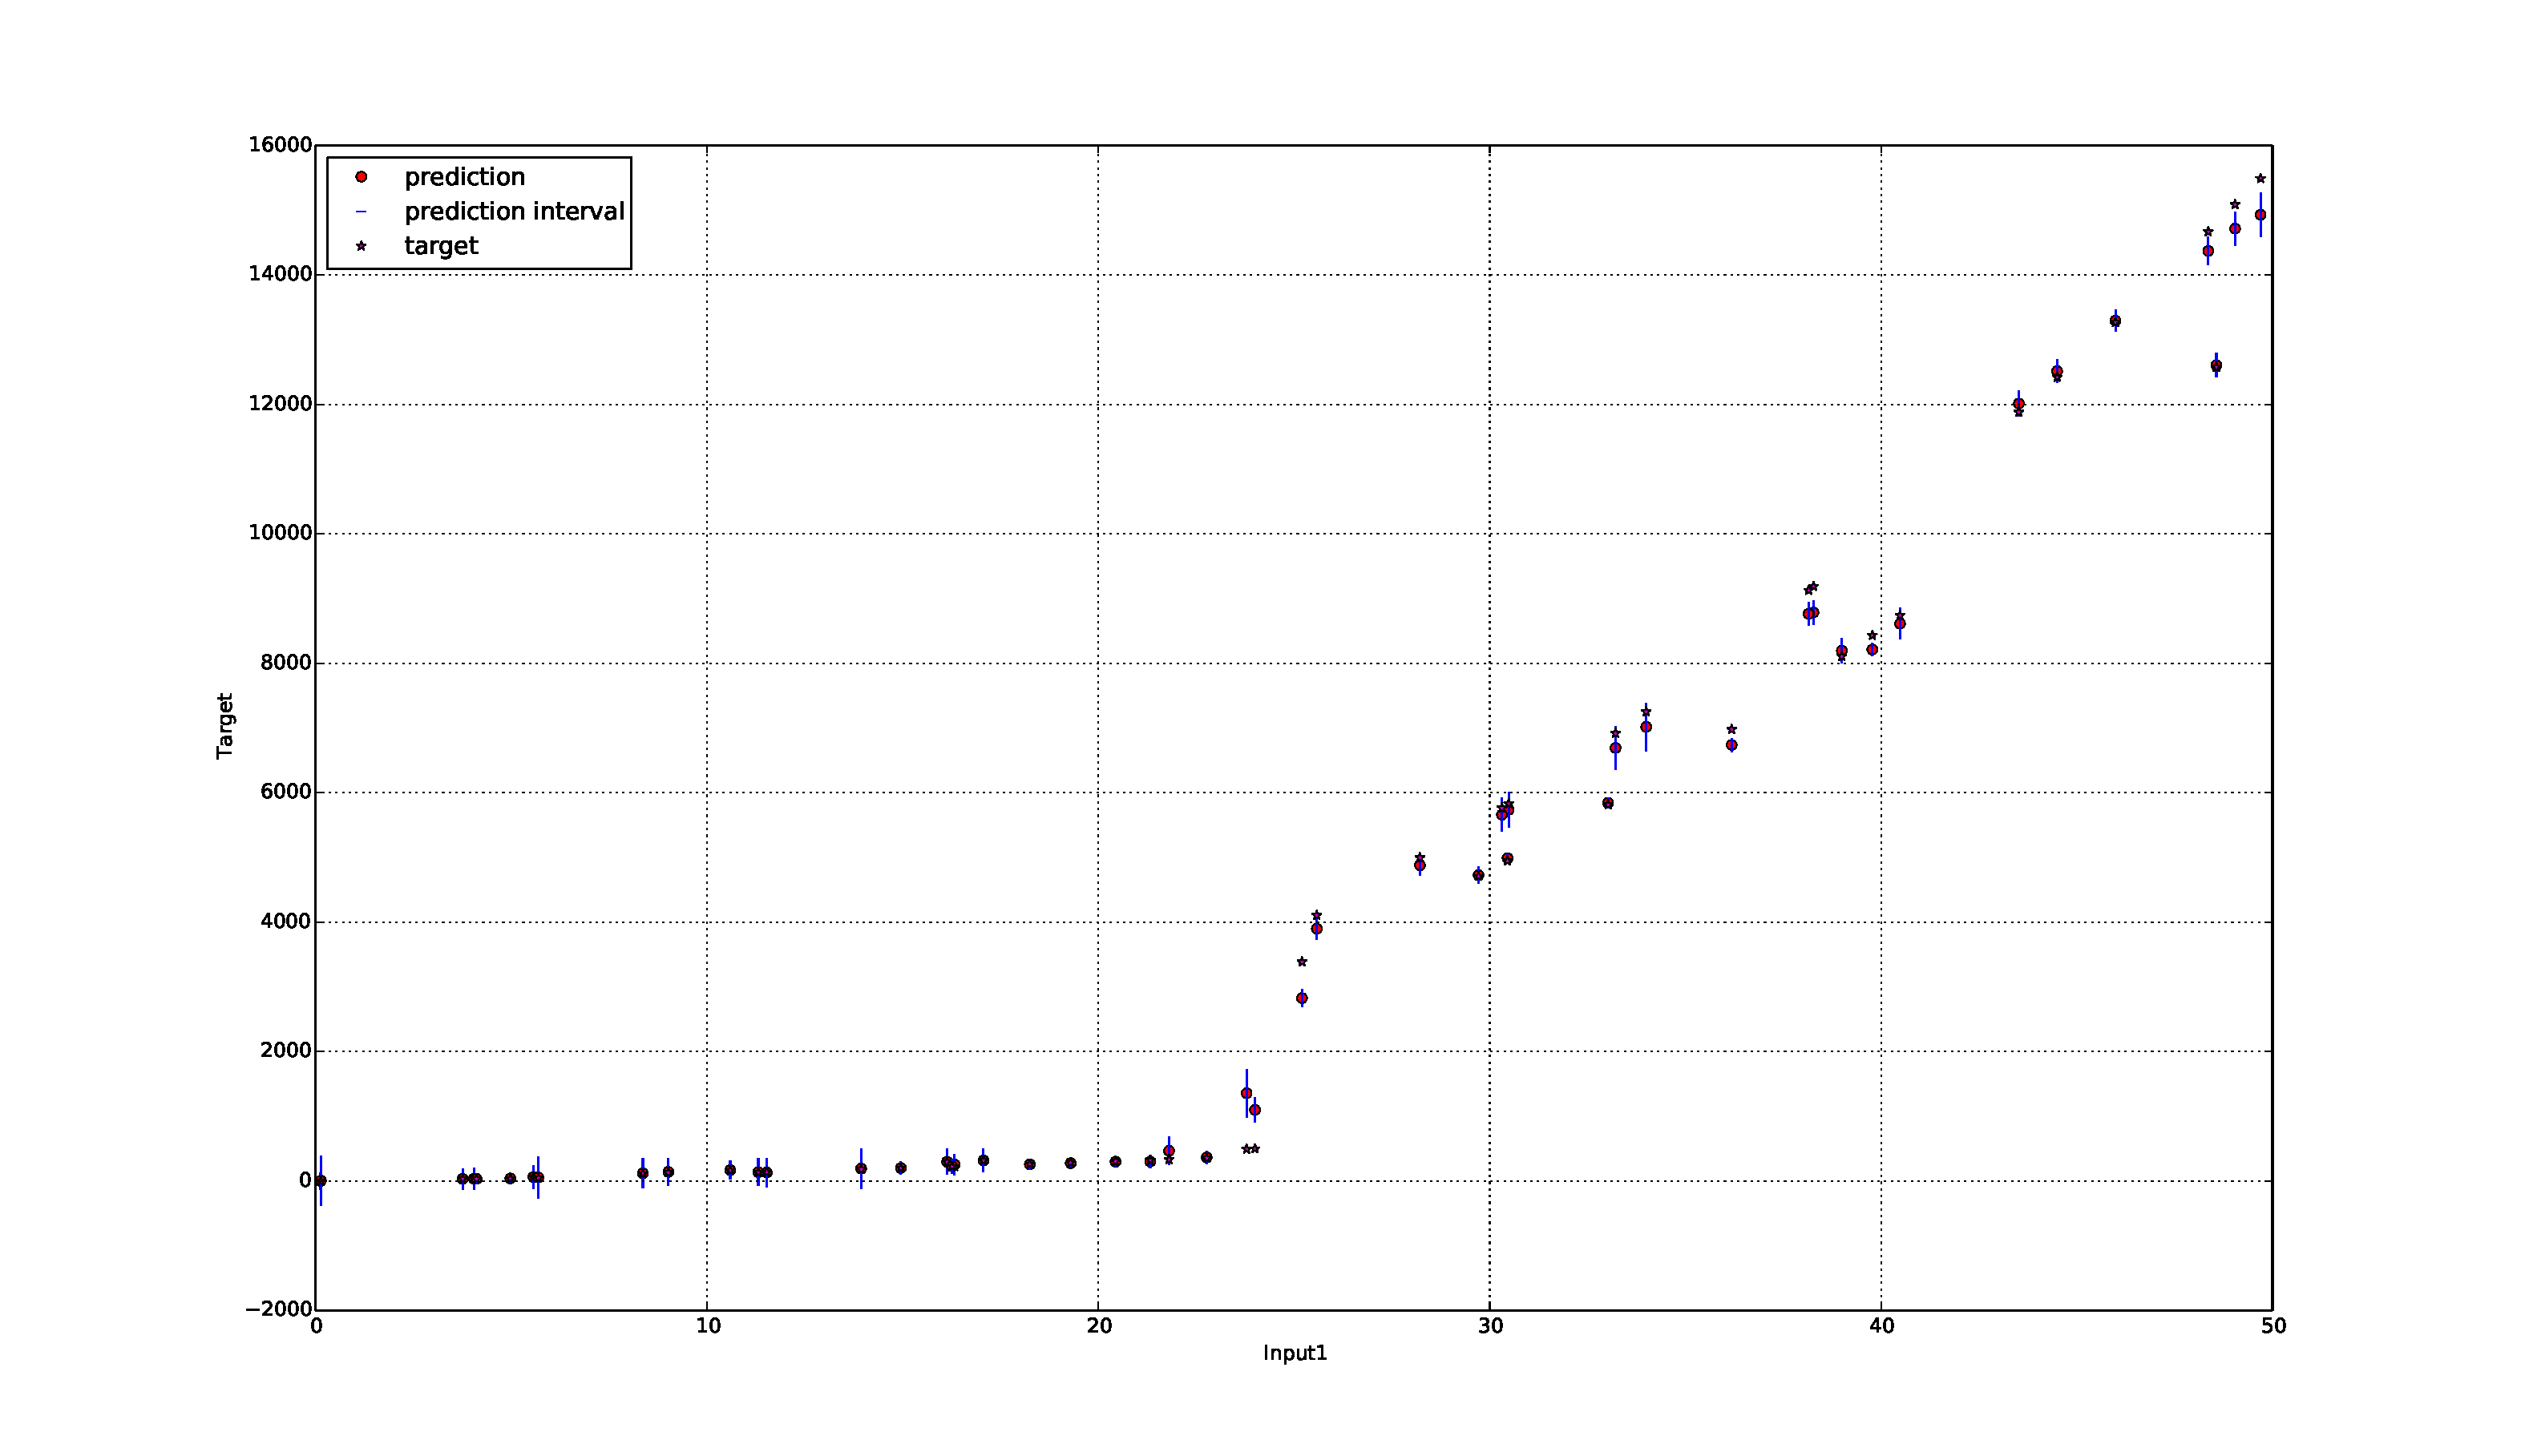
\includegraphics[width=\linewidth]{./Figures/sampled_50_predictions_kreg_ws64_SYNTH_D_CD_2000_1_50_3_23.pdf}
  \caption{\texttt{KernelRegression\_WS64} tested on \texttt{SYNTH\_D\_CD\_2000\_1\_50\_3\_23}. 50 sample predictions along with their corresponding targets and prediction intervals are shown}
 \label{fig:sampled_50_predictions_kreg_ws64_SYNTH_D_CD_2000_1_50_3_23}
\end{figure}

\begin{figure}[htbp]
  \centering
    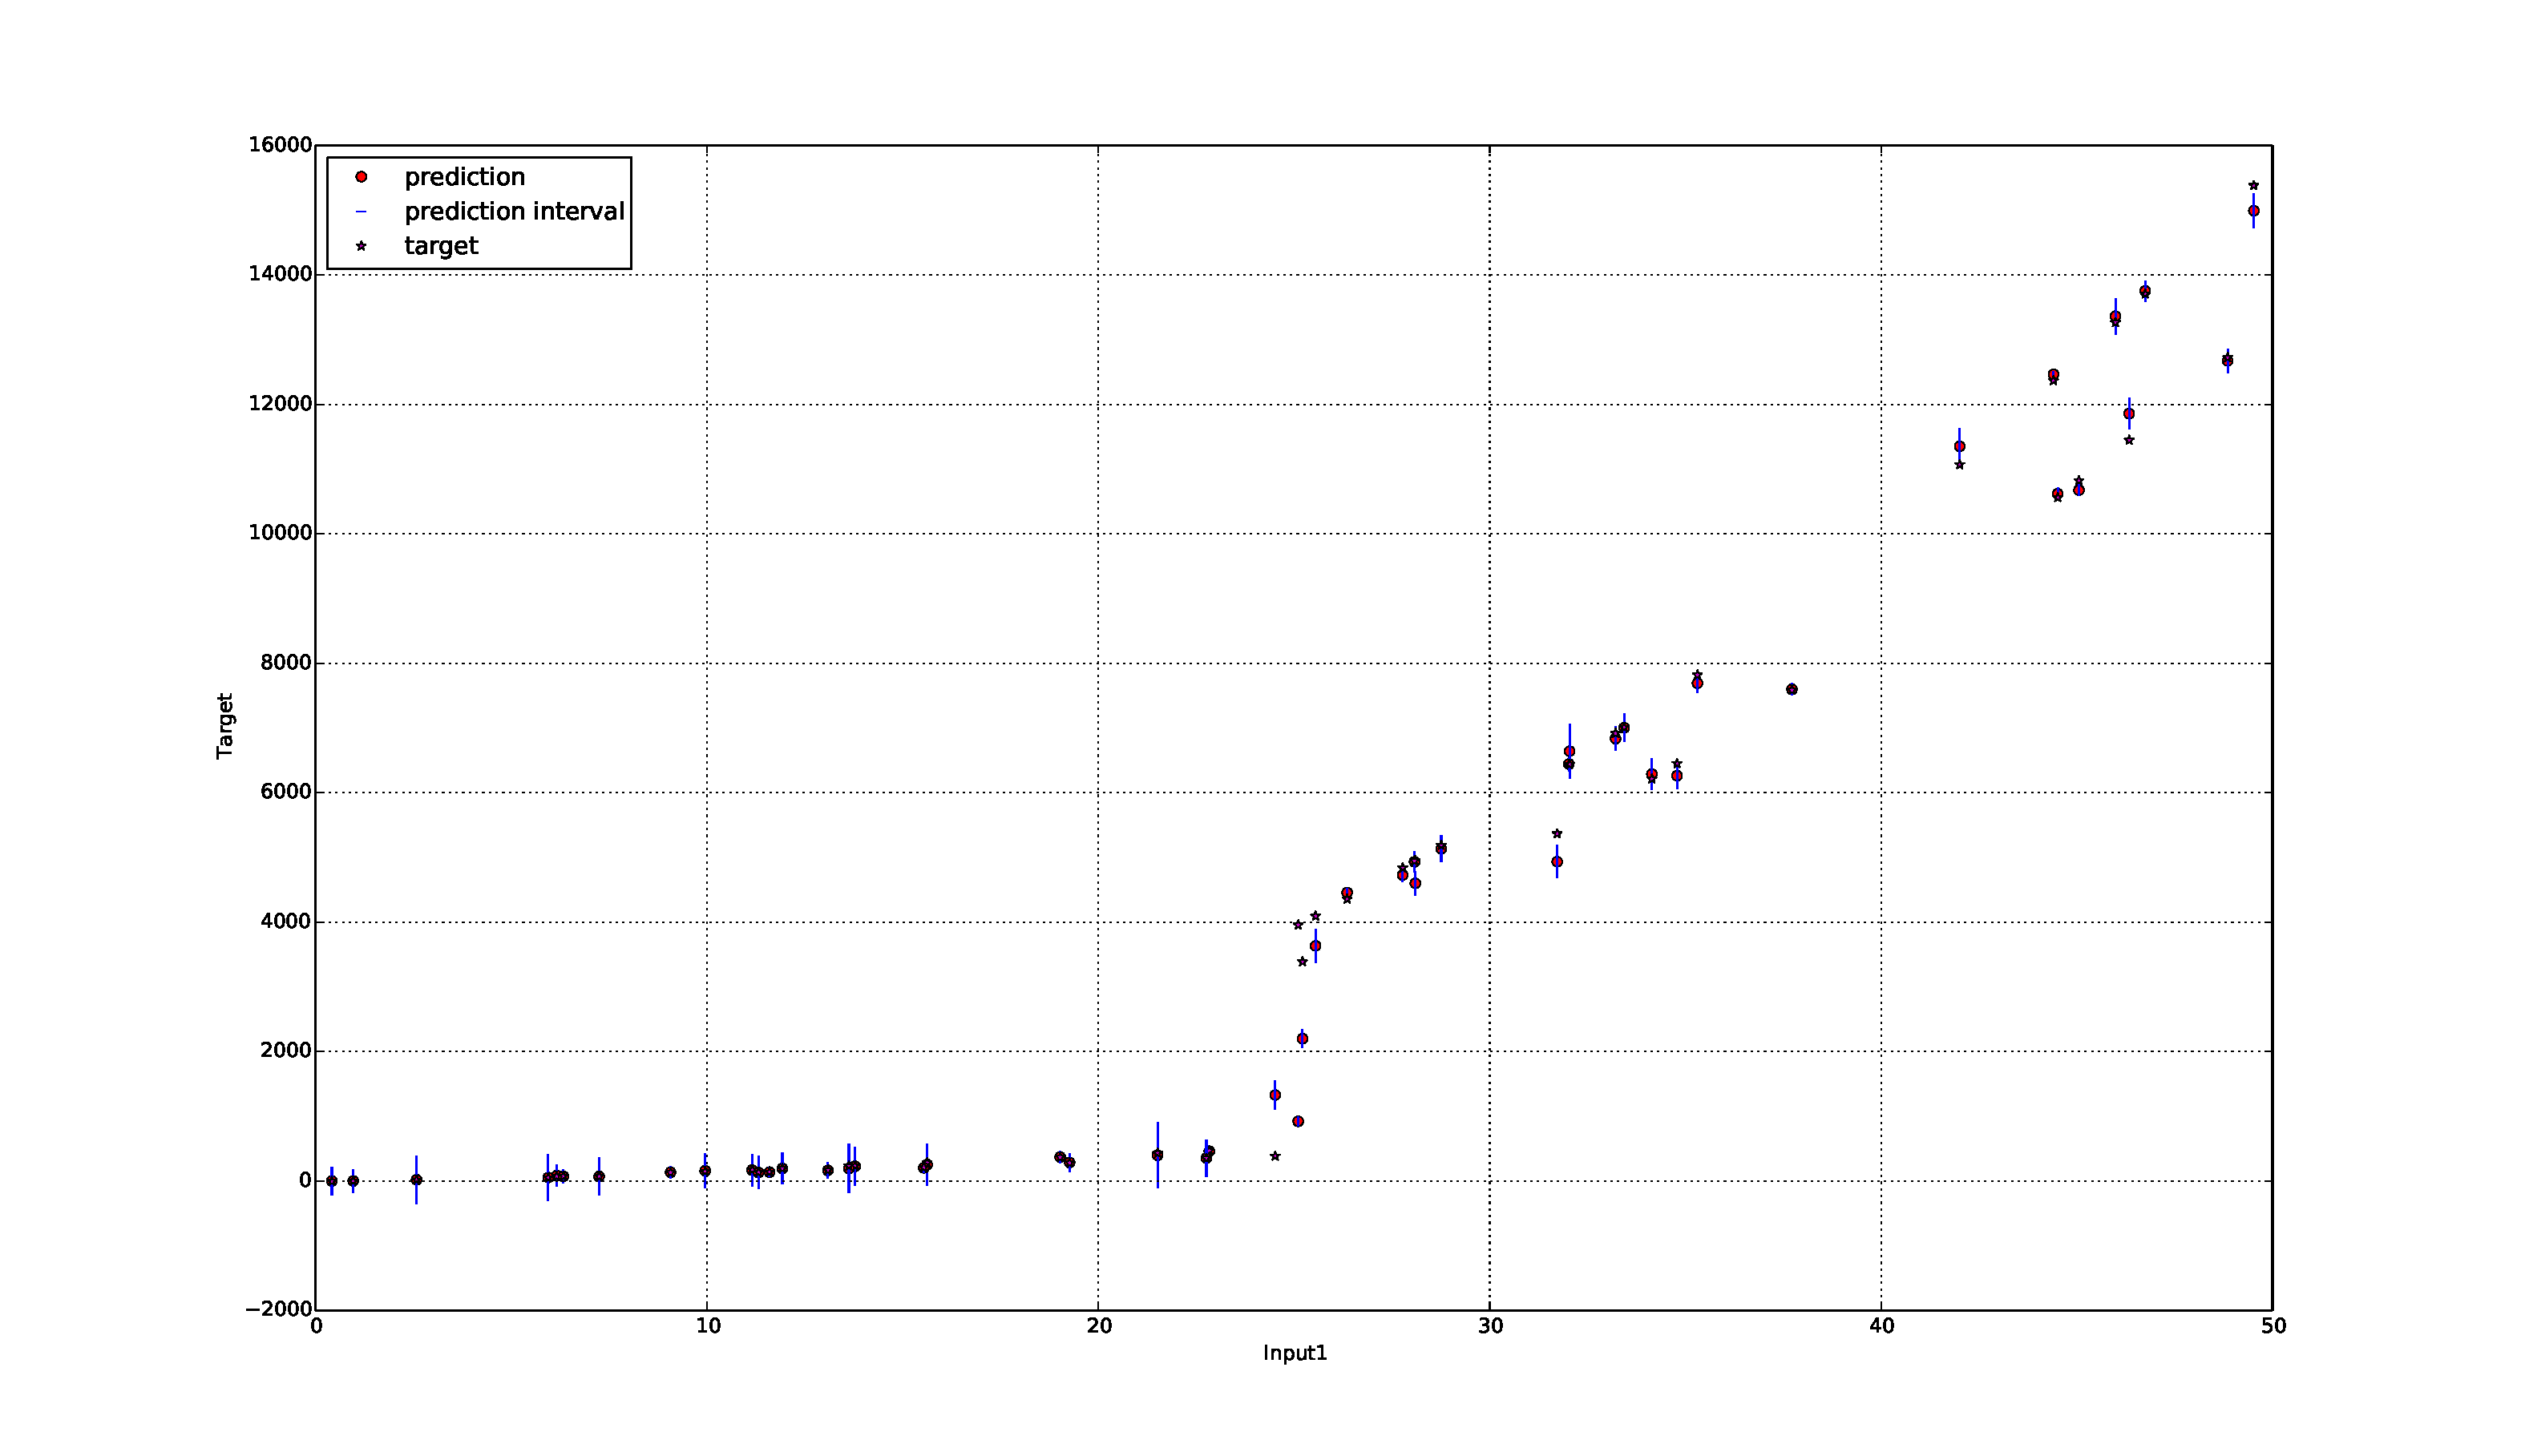
\includegraphics[width=\linewidth]{./Figures/sampled_50_predictions_kreg_ws96_SYNTH_D_CD_2000_1_50_3_23.pdf}
  \caption{\texttt{KernelRegression\_WS96} tested on \texttt{SYNTH\_D\_CD\_2000\_1\_50\_3\_23}. 50 sample predictions along with their corresponding targets and prediction intervals are shown}
 \label{fig:sampled_50_predictions_kreg_ws96_SYNTH_D_CD_2000_1_50_3_23}
\end{figure}

When \ref{fig:sampled_50_predictions_kreg_ws64_SYNTH_D_CD_2000_1_50_3_23} and \ref{fig:sampled_50_predictions_kreg_ws96_SYNTH_D_CD_2000_1_50_3_23} are examined carefully, what is observed from the figures is that although the point predictions are pretty close to targets, the prediction bounds around them are so tight that they cannot reach the target points for significantly many of the $50$ points sampled. However, this is not an unavoidable problem unlike the prediction interval issues with sliding windowed parametric models on the data from discontinuous functions or forgetting-factor based parametric models in general. A possible solution to this problem arbitrarily extend the reach of the prediction bounds. This will surely result in an increase in \texttt{SAIW} but since \texttt{SAIW} values are relatively low as seen in \ref{fig:gen_alg_comparison} ($0.33$ for both learners), this interval extension method can be applied to some extent without trouble. From a theoretical point of view, extending the interval between the prediction bounds by multiplying the length between the bounds and the point prediction by some constant is equivalent of asking the prediction bound estimation method to return the bounds with a higher confidence parameter than the \textit{usual} $95\%$.

Following the the idea proposed above, $2$ \texttt{KernelRegression} learners were again tested on $576$ stream simulations after modifying the prediction bound estimation mechanism so that it returns the confidence intervals\footnote{Note that confidence intervals instead of prediction intervals are used as the prediction bounds for \texttt{KernelRegression} learners.} with $99.9\%$ confidence instead of $95\%$. The modified \texttt{KernelRegression} learners are referred to as \texttt{KernelRegression\_HighConf}.

\begin{figure}[htbp]
  \centering
    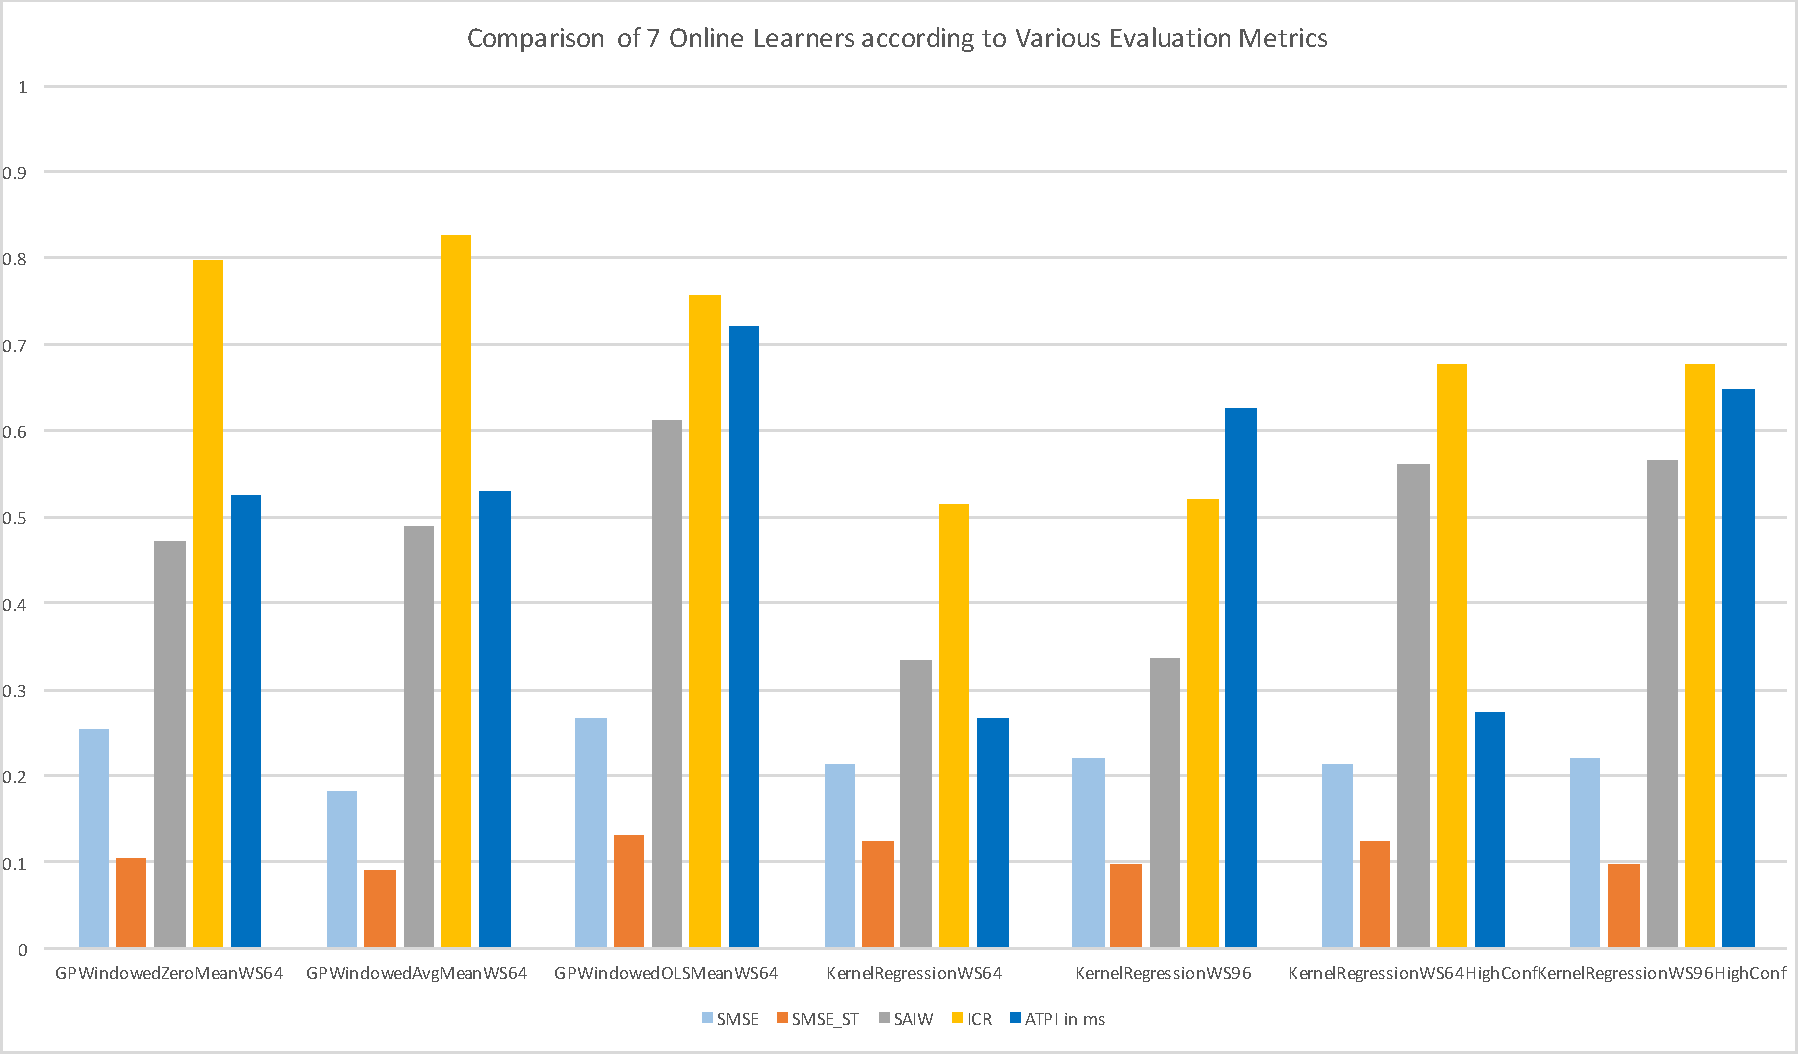
\includegraphics[width=\linewidth]{./Figures/final_7_comparison.pdf}
  \caption{Comparison of \texttt{SMSE}, \texttt{SMSE\_ST}, \texttt{ICR} and \texttt{ATPI} statistics for 7 different learners whose full codenames are shown on the x- axis tested on 576 streams}
  \label{fig:final_7_comparison}
\end{figure}

Figure \ref{fig:final_7_comparison}, shows various statistics of the both original and modified \texttt{KernelRegression} learners along with the \texttt{GPRegression} learners for comparison. In the graph, it appears that all $7$ learners were pretty accurate keeping \texttt{SMSE} and \texttt{SMSE\_ST} scores below $0.25$ and $0.15$ respectively. \texttt{GPRegressionAvgMean} seems to be a bit more accurate than the rest. It is followed by the \texttt{KernelRegressionWS96} (both versions) and \texttt{GPRegressionZeroMean}. \texttt{GPRegressionOLSMean} trails behind the other $6$ learners in terms of accuracy. With the prediction interval modification on the \texttt{KernelRegression} algorithms, target variable coverage scores of \texttt{KernelRegression} learners are brought to the same levels of that of \texttt{GPRegression} learners. This unsurprisingly resulted in increasing \texttt{SAIW} scores although they did not pass $0.6$ meaning the average gap between prediction bounds were still not too high. In terms of the prediction time per item, none of the $7$ learners spend more than $0.75$ ms per item on average. \texttt{KernelRegressionWS64}, processing a stream item $0.27$ ms on average, appears to be the quickest learner while \texttt{GPRegressionOLSMean} is the slowest one with \texttt{APTI} of $0.72$ ms.

Modifying the \texttt{KernelRegression} learners from the list \ref{final_11} as discussed above and eliminating the unsuitable ones, $5$ learners out of the initial $52$ are left. These are listed as follows:

\begin{itemize}
\label{final_5}
\item \texttt{GPRegressionZeroMean\_WS64}
\item \texttt{GPRegressionAvgMean\_WS64}
\item \texttt{GPRegressionOLSMean\_WS64}
\item \texttt{KernelRegression\_HighConf\_WS64}
\item \texttt{KernelRegression\_HighConf\_WS96}
\end{itemize}

Next, using the advantage of having synthetic test data, how the accuracy, prediction bounds quality and time-efficiency change with the changing noise levels, input dimensionality\footnote{Note that analyzing the experiment results by the input dimensionality would be possible with the real measurement data as well.} and discontinuity of the function used for mocking the streaming data.

\begin{figure}[htbp]
  \centering
    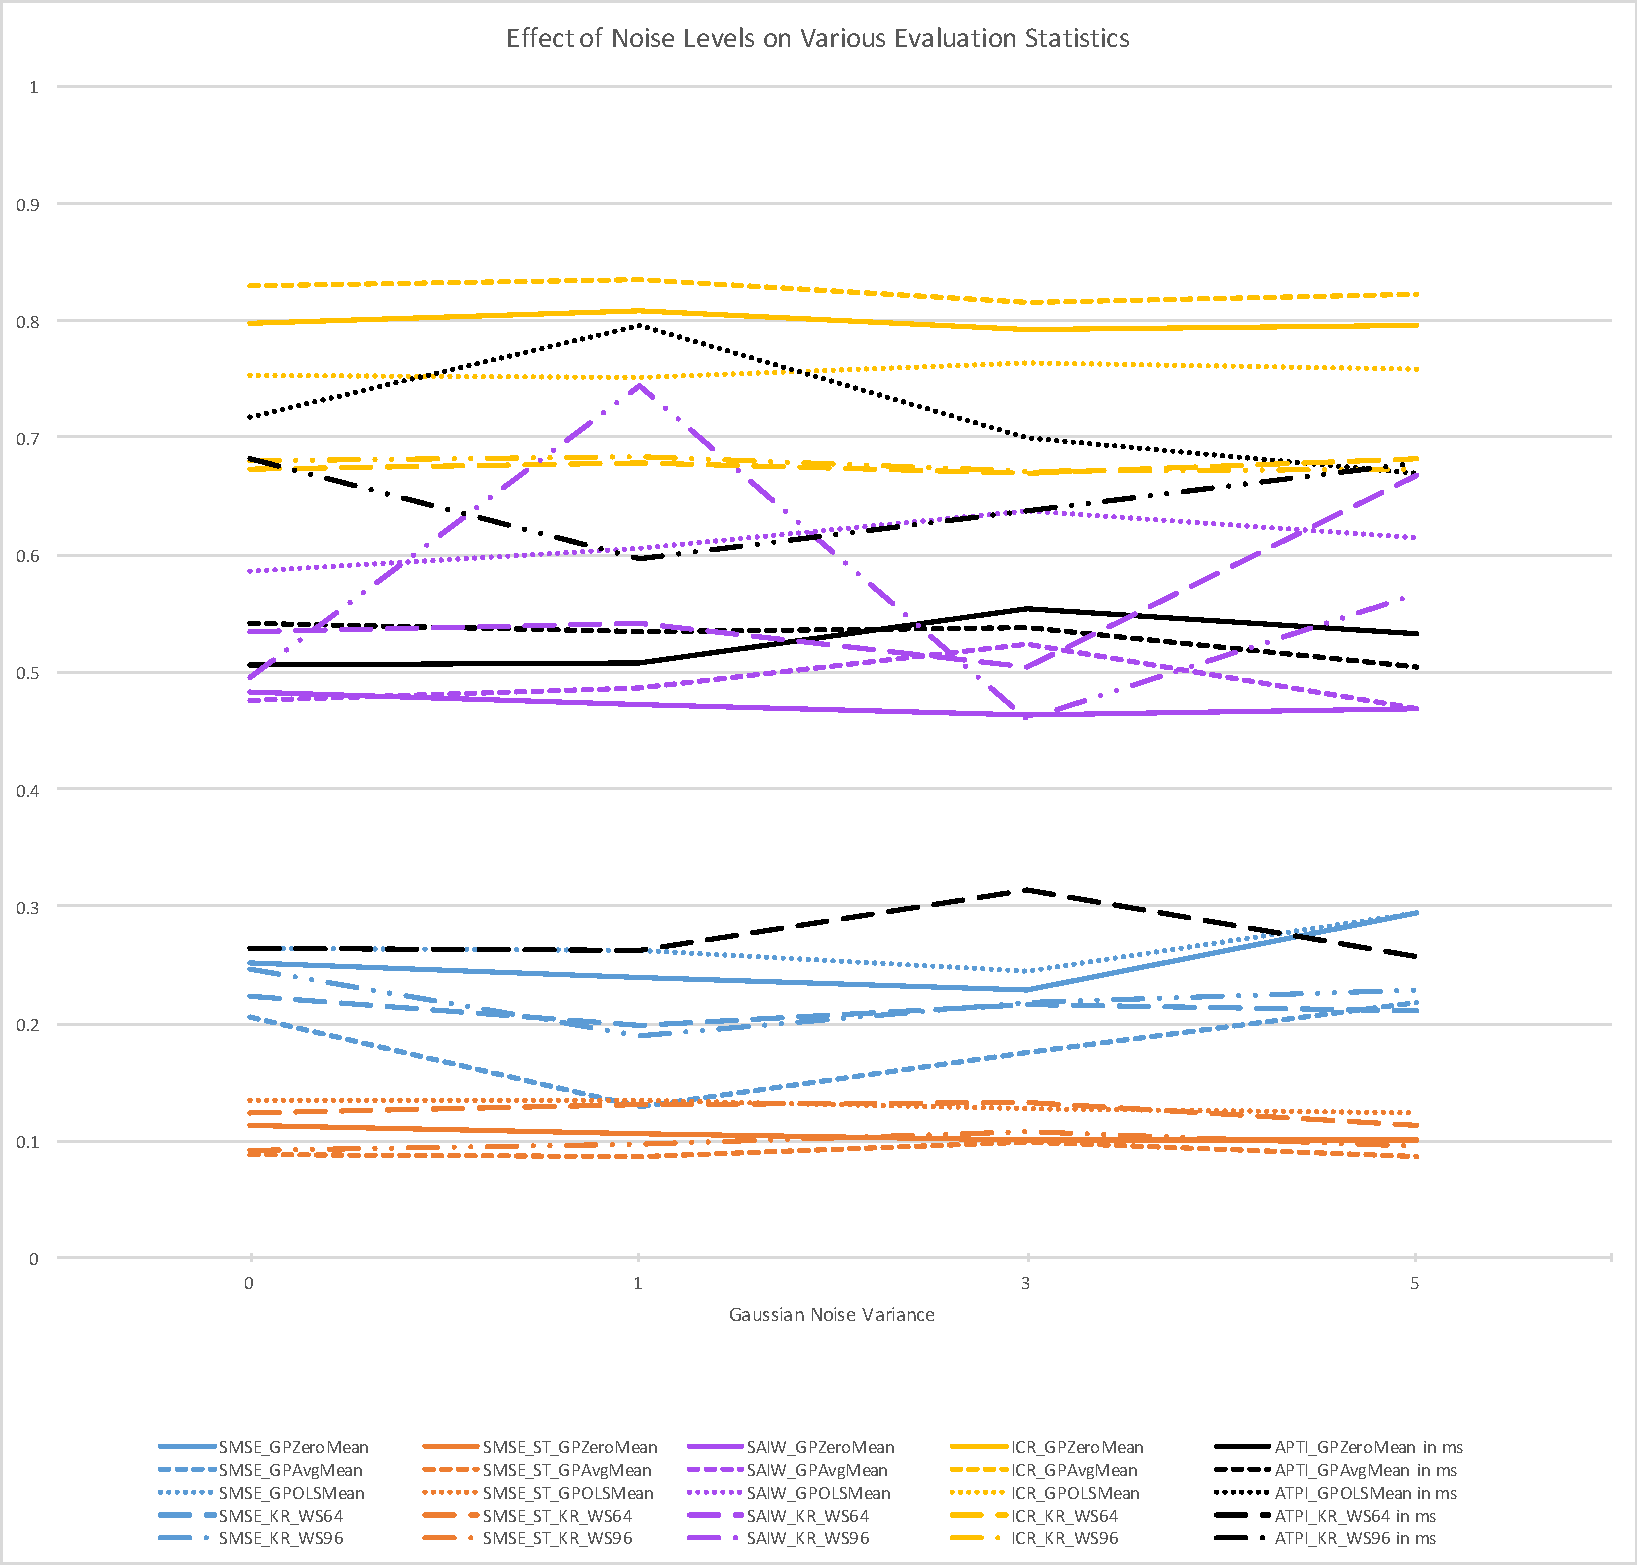
\includegraphics[width=\linewidth]{./Figures/noise_effect_on_final_5.pdf}
  \caption{Visualization of how \texttt{SMSE}, \texttt{SMSE\_ST}, \texttt{ICR} and \texttt{ATPI} scores change as the measurement noise increases for 5 different learners listed in \ref{final_5}. The results are aggregated over 144 stream simulations for each noise level}
  \label{fig:noise_effect_on_final_5}
\end{figure}

Figure \ref{fig:noise_effect_on_final_5} shows that the average stable and general accuracy of the learners \textit{remarkably} did not increase with the increasing noise levels. This allows for a quick yet an important conclusion about the online learning algorithms employed: More measurement noise does not mean more error. In other words, the online learners employed are robust to noise.

Average prediction bounds coverage also remained nearly the same when the noise variance is increased from $0.0$ (no noise) to $5.0$. Moreover, in terms of the average width of the intervals set by the prediction bounds, \texttt{GPRegression} learners were almost insensitive to noise exhibiting small fluctuations with the increasing noise. As for \texttt{KernelRegression}, the \texttt{SAIW} statistic of the learner with the sliding-window size of $96$ is funky. It jumps to high levels when switching from no-noise to the minimal noise as indicated by the double dotted dashed line. Moreover, It decreases when the noise is set to a moderate level and then increases again when the noise is high. This jumpy pattern does not allow to draw a confident conclusion about the prediction bounds behavior with the changing noise variance for the \texttt{KernelRegression\_HighConfidence\_WS96}. The other \texttt{KernelRegression} learner from the list \ref{final_5} seems to represent the same pattern but with the smaller amounts of \textit{jumps} from one noise level to another. 

As indicated by the black lines in the Figure \ref{fig:noise_effect_on_final_5}, average time spent for one stream item also fluctuates with the increasing noise. Similar to the prediction bounds behavior of \texttt{KernelRegression}, black lines for the all $5$ learners do not represent a steady trend making it hard to infer a relation between the average processing time per item and the noise level. However, it is not surprising as the underlying mechanism that produced this experiment data, being the execution flow of the learning algorithms that is partially controlled by the drift detection mechanism that modifies the internal state of the learners causing update and tuning operations that increases the item processing time to be fired or inhibited, is complex. 

\begin{figure}[htbp]
  \centering
    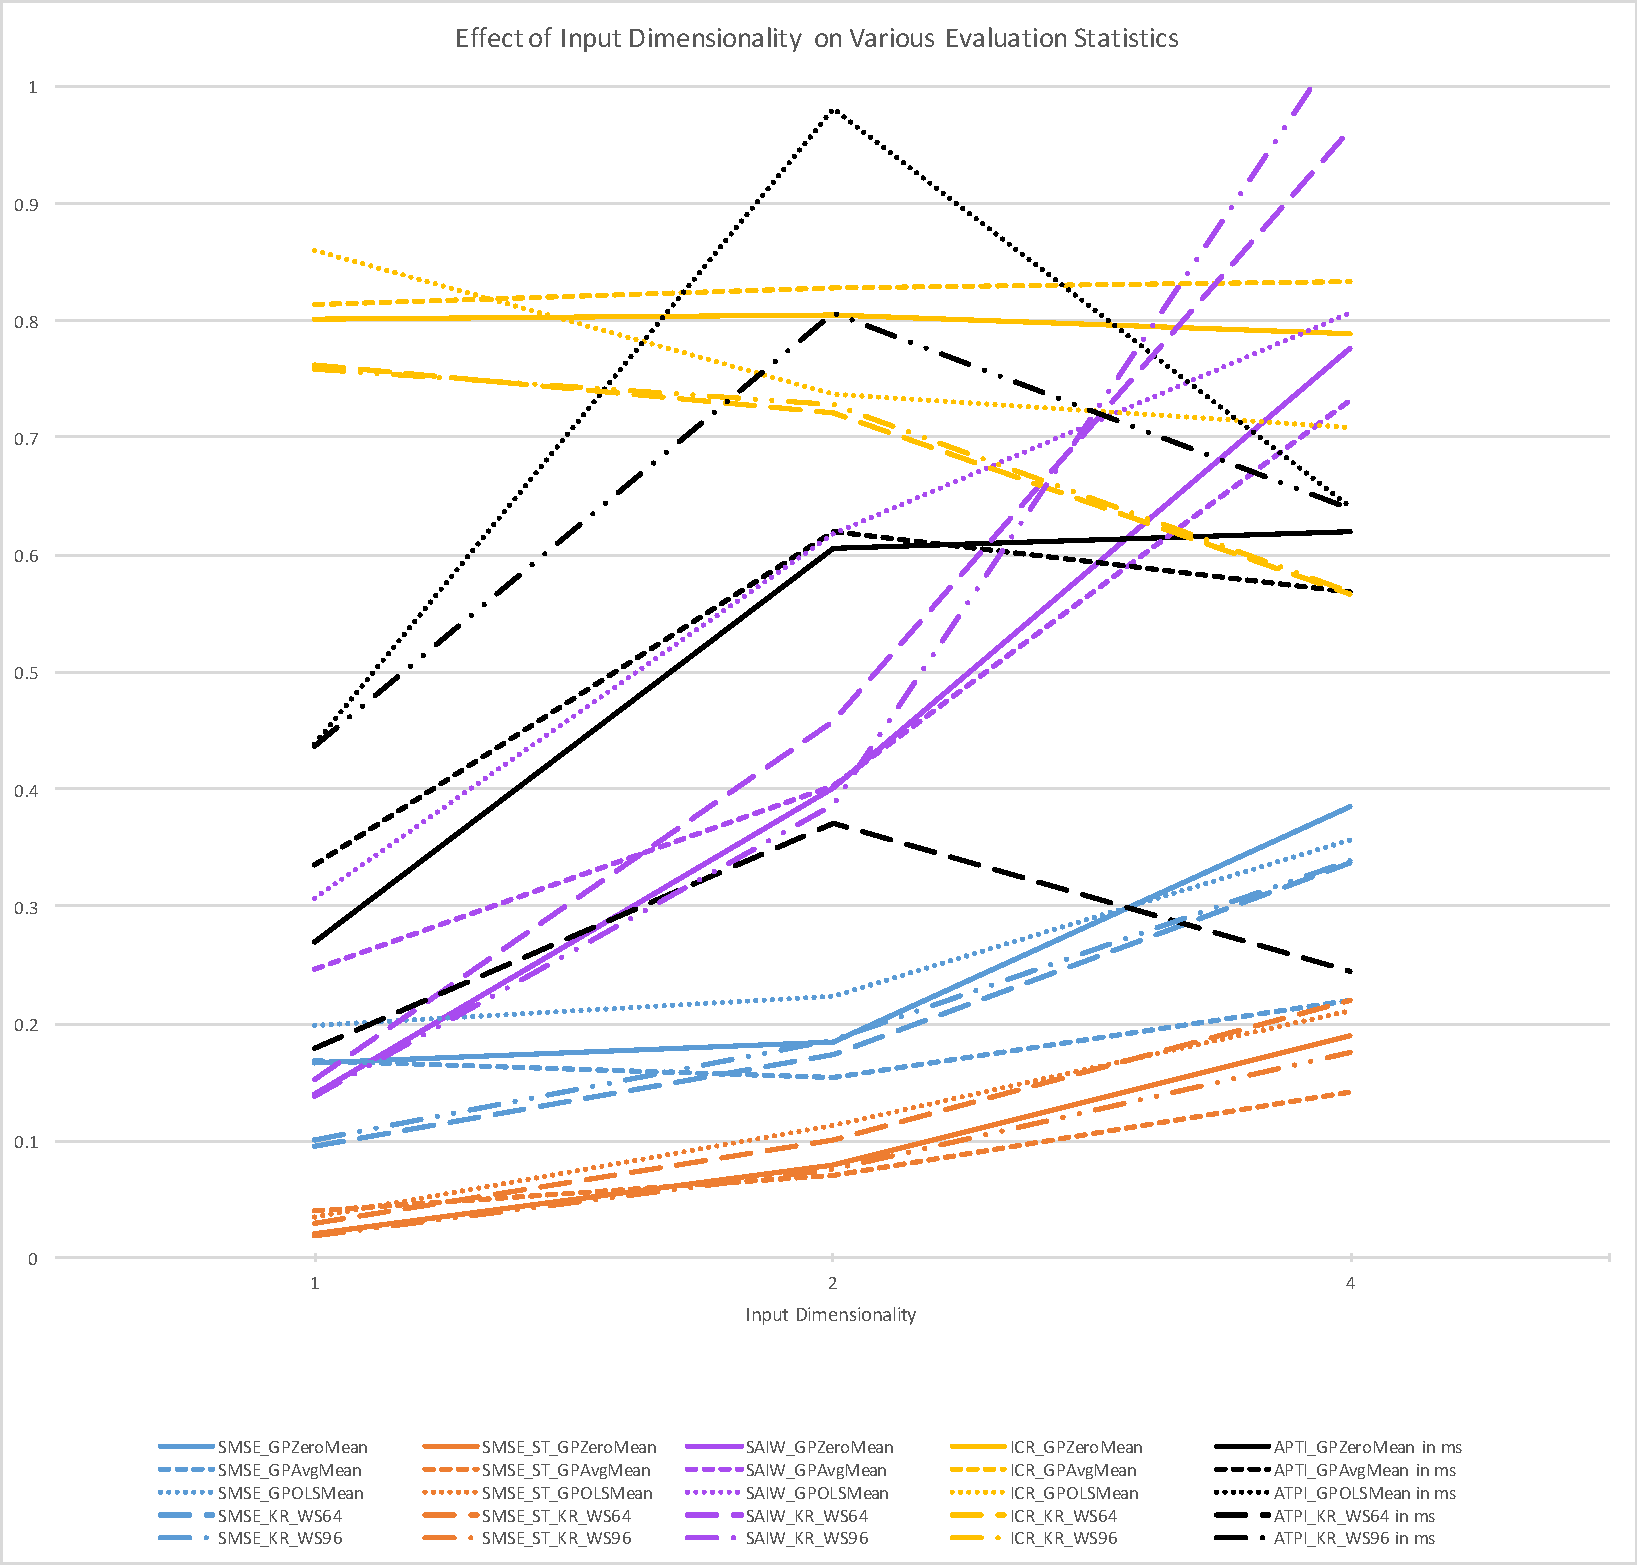
\includegraphics[width=\linewidth]{./Figures/inpdim_effect_on_final_5.pdf}
  \caption{Visualization of how \texttt{SMSE}, \texttt{SMSE\_ST}, \texttt{ICR} and \texttt{ATPI} scores change as the input dimensionality increases for 5 different learners listed in \ref{final_5}. The results are aggregated over 144, 216 and 216 stream simulations for input dimensionalities of 1,2 and 4 respectively}
  \label{fig:inpdim_effect_on_final_5}
\end{figure}

In Figure \ref{fig:inpdim_effect_on_final_5}, as observed in the previous more general experiment results presented in \ref{fig:curse_of_dim}, average general and stable accuracy seem to increase with the growing number of predictor variables.  As for the averaged \texttt{ICR} values, learners except for the \texttt{KernelRegression\_HighConf\_WS64} and \texttt{KernelRegression\_HighConf\_WS96} that appeared to be input dimensionality-oblivious, all exhibited a drop when the input dimensionality increased. This means that the average coverage of the prediction bounds decreases when the number of predictors in the input increases. This drop is more more remarkable in the case of \texttt{KernelRegression} learners and especially when the number of predictors are bumped up to $4$ from $2$. As for, \texttt{GPRegressionOLSMean\_WS64}, the prediction bound coverage drop did not make the learner unemployable but it definitely shows that \texttt{GPRegressionOLSMean\_WS64} is not robust to growing input-dimensionality. This is expected as unlike the other \texttt{GPRegression} learners, it partially uses Ordinary Least Squares algorithm in addition to Gaussian Processes.

A more striking observation than the \texttt{ICR} drop with the growing number of predictors is the dramatic increase in \texttt{SAIW} under the same conditions. Without an exception, the average gap between the upper and the lower prediction bounds that online learners estimate significantly increases as the number of dimensions in the input is raised. This is even more exaggerated in the case of \texttt{GPRegressionZeroMean\_WS64} and \texttt{GPRegressionAvgMean\_WS96}. These results are not totally surprising when the mechanism used to estimate prediction bounds are understood. These are covered in Chapter \ref{Chapter4}.

When the change in the average time spent for each data stream item as the number of predictors increase are examined, a pattern which all 5 learners exhibit is observed. The \texttt{ATPI} first significantly increases when the input dimensionality is raised from $1$ to $2$, then, it either remained almost same or decreased when it the number of predictors are doubled to $4$ from $2$. The first bump is rather understandable as the decrease in the accuracy might have caused the error-triggered update and tuning mechanism to fire more often resulting in increased processing time per stream item. The explanation for the mentioned \textit{drop} in the processing time is somewhat involved and it lies in the implementation details of the error-triggered update and tuning mechanism that is covered in \ref{section:online_learner_semantics}. In short, the magnitude of the increase in error terms was not high enough for error-triggered update and tuning mechanism to kick in in the case of four dimensional input space as frequently as it does with the streams with data points having two predictors.

\begin{figure}[htbp]
  \centering
    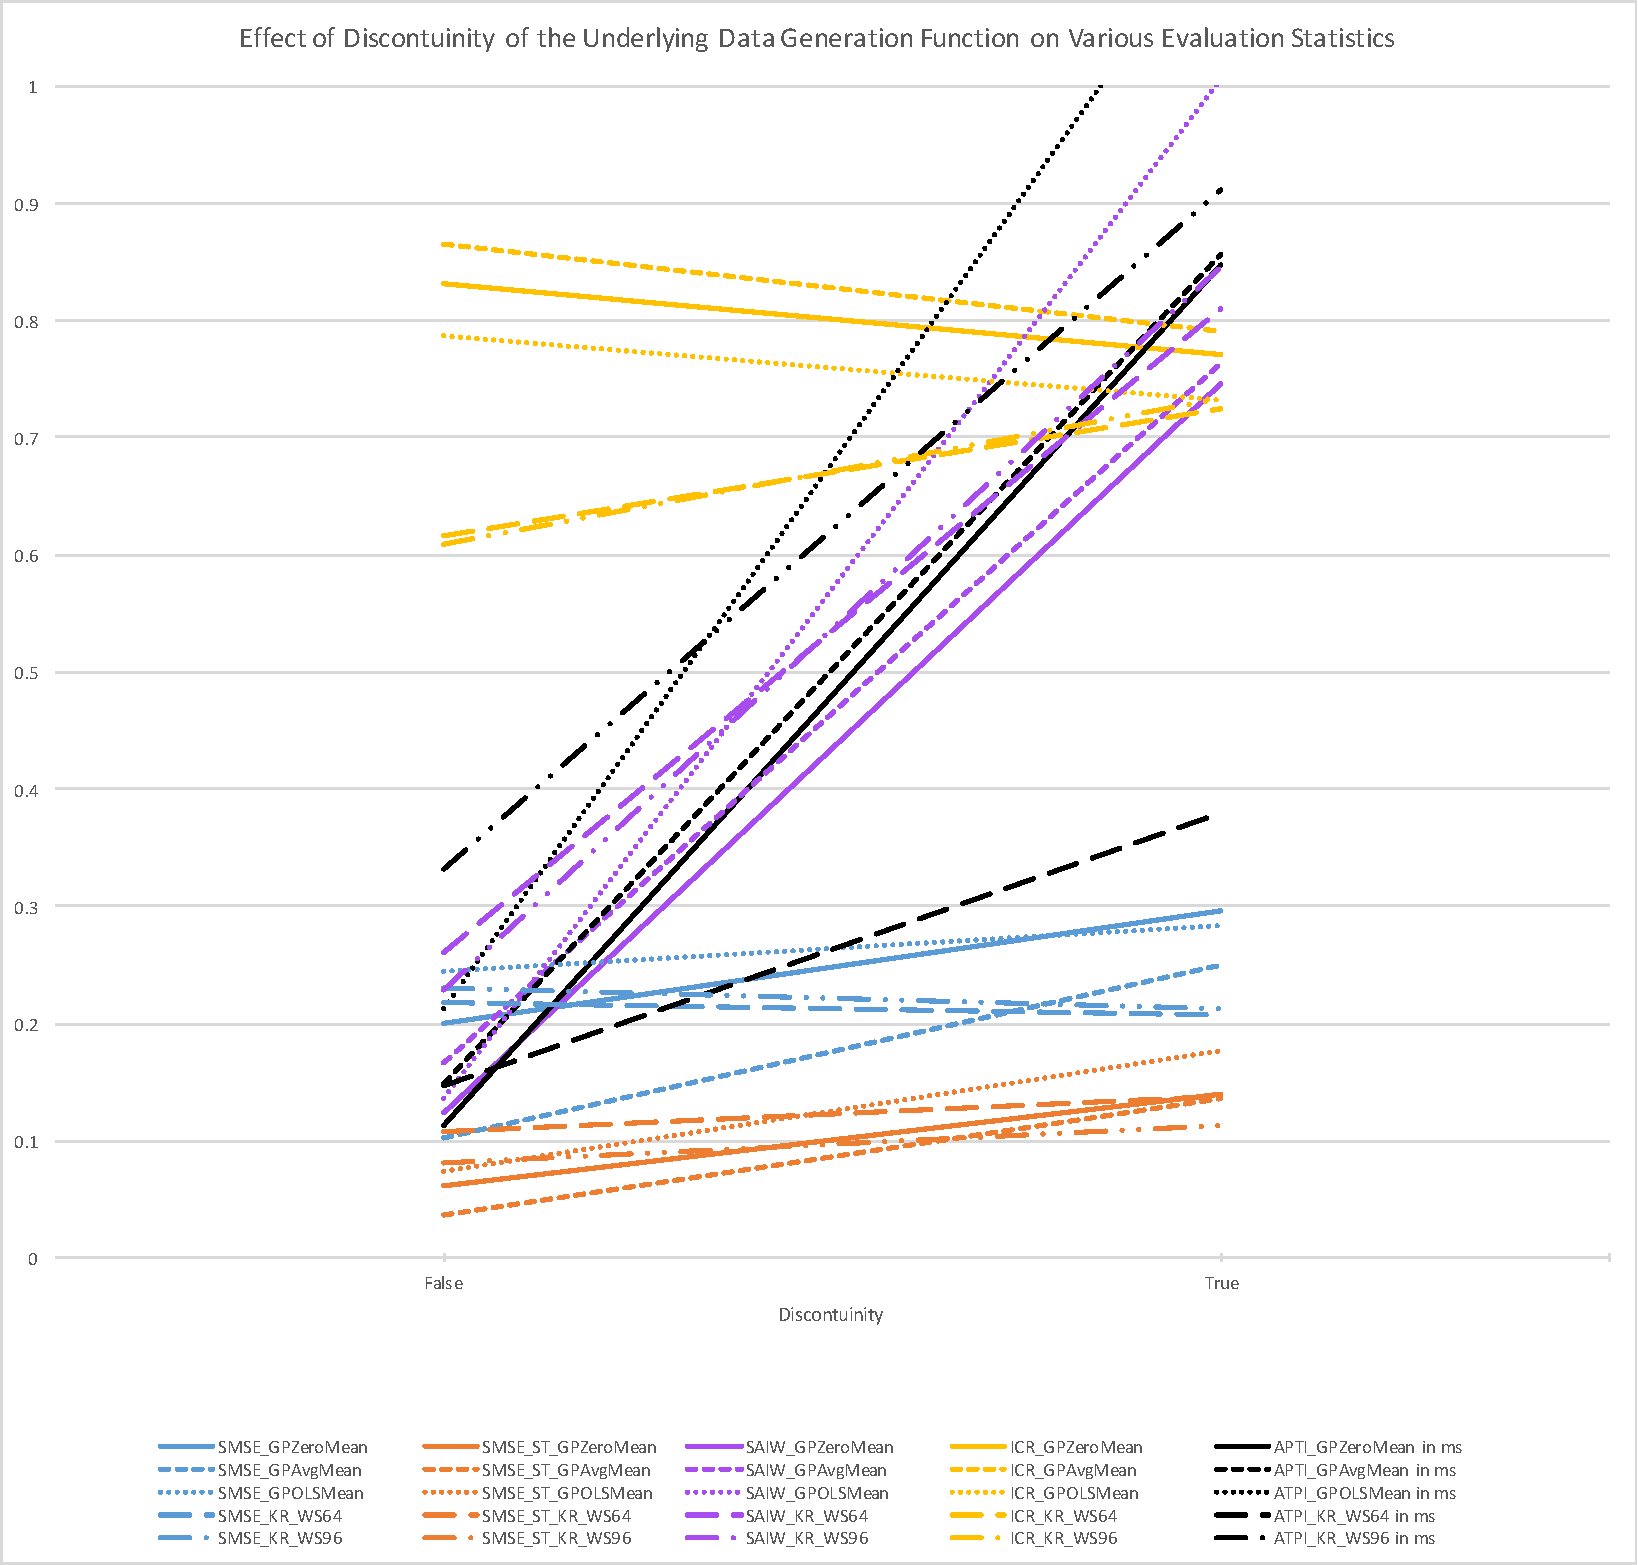
\includegraphics[width=\linewidth]{./Figures/disc_effect_on_final_5.pdf}
  \caption{Visualization of how discontinuity of the function used to generate data sets which the streams are simulated from affects \texttt{SMSE}, \texttt{SMSE\_ST}, \texttt{ICR} and \texttt{ATPI} scores for 5 different learners listed in \ref{final_5}. The results are aggregated over 276 discontinuous and 276 continuous cases.}
  \label{fig:disc_effect_on_final_5}
\end{figure}

The Graph \ref{fig:disc_effect_on_final_5} shows that all the statistics except for \texttt{ICR} are higher in the discontinuous case than in the continuous case\footnote{continuous and discontinuous case refer to the the function that generated the data set which the test streams are simulated from having discontinuity or not.}. Increasing \texttt{SAIW} and \texttt{APTI} can be explained by the descent increase in the \texttt{SMSE} and \texttt{SMSE\_ST} as lower accuracy is the result of higher errors that also cause the gaps between the prediction bounds to grow larger to avoid declining \texttt{ICR} scores and activating the error-triggered update-tuning mechanism more often. As for \texttt{ICR} scores, they did not change as dramatically as the other statistics. \texttt{GPRegression} learners had lowered \texttt{ICR} when switched from continuous case to discontinuous case while \texttt{KernelRegression} learners improved their \texttt{ICR} scores. This obviously suggests that the different behaviour of the prediction bounds estimated by the different learners using different learning algorithms is linked to their different prediction bound estimation mechanism. However, why exactly the discontinuity of the data generation function has boosted the prediction bounds coverage of the learners of one learning algorithm family as well as the reason why it dropped that of the learners of the other learning algorithm family remain an open question.

\subsection{Visualization of the cost function approximations by the shortlisted learners on synthetic data sets}

In this subsection, predictions of the learners listed in \ref{final_5} on $2$  simulated streams and their visual comparison to the layout of the data points in the stream together with their corresponding target points are presented. The chosen datasets used for the stream simulations are all generated by discontinuous functions. Moreover, the streams on which the learners are tested feature concept drifts. As a result, when the data points in the test streams are visualized, four partial functions constituting one discontinuous function per stream appear. The motivation for using concept-drifting data streams simulated from datasets generated by discontinuous functions is that the stream learning scenario that Ocelot's runtime operator estimator module will confront are mostly expected to be similar. 

\begin{figure}[htbp]
  \centering
    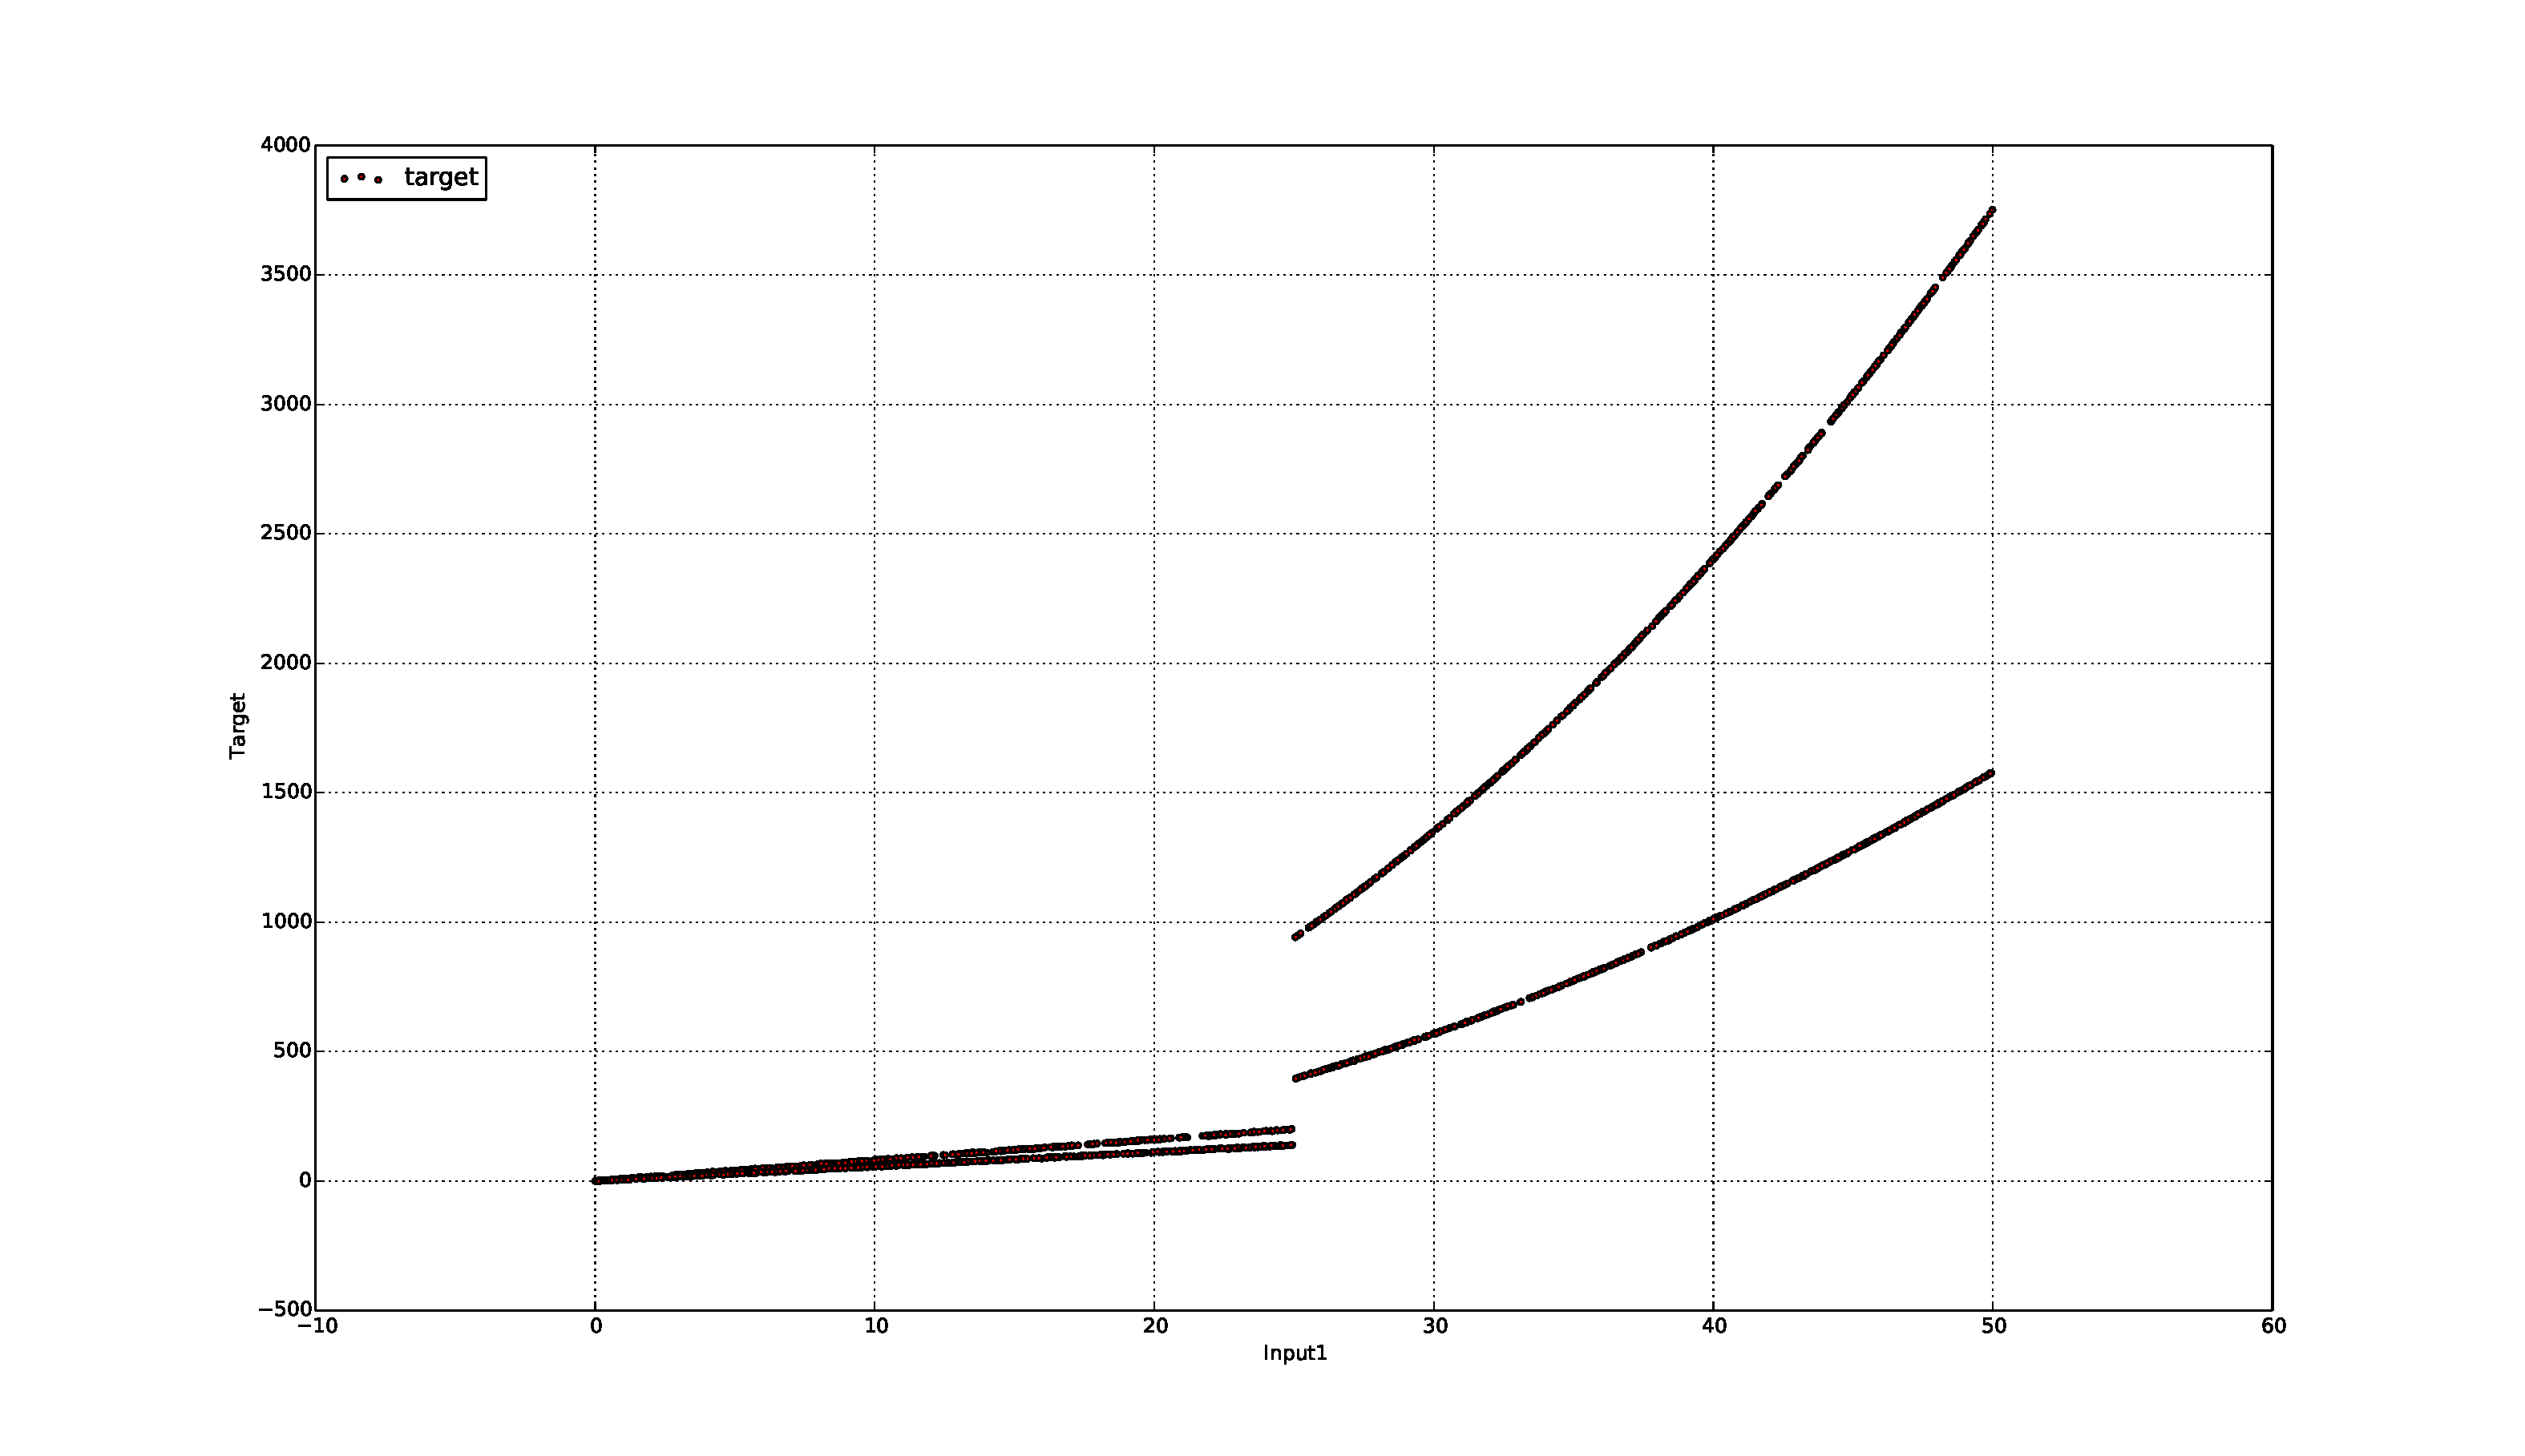
\includegraphics[width=\linewidth]{./Figures/ref_func_SYNTH_D_CD_2000_1_50_1_13.pdf}
  \caption{Visualization of the stream simulated from dataset} \texttt{SYNTH\_D\_CD\_2000\_1\_50\_1\_13}
  \label{fig:ref_func_SYNTH_D_CD_2000_1_50_1_13}
\end{figure}

\begin{figure}[htbp]
  \centering
    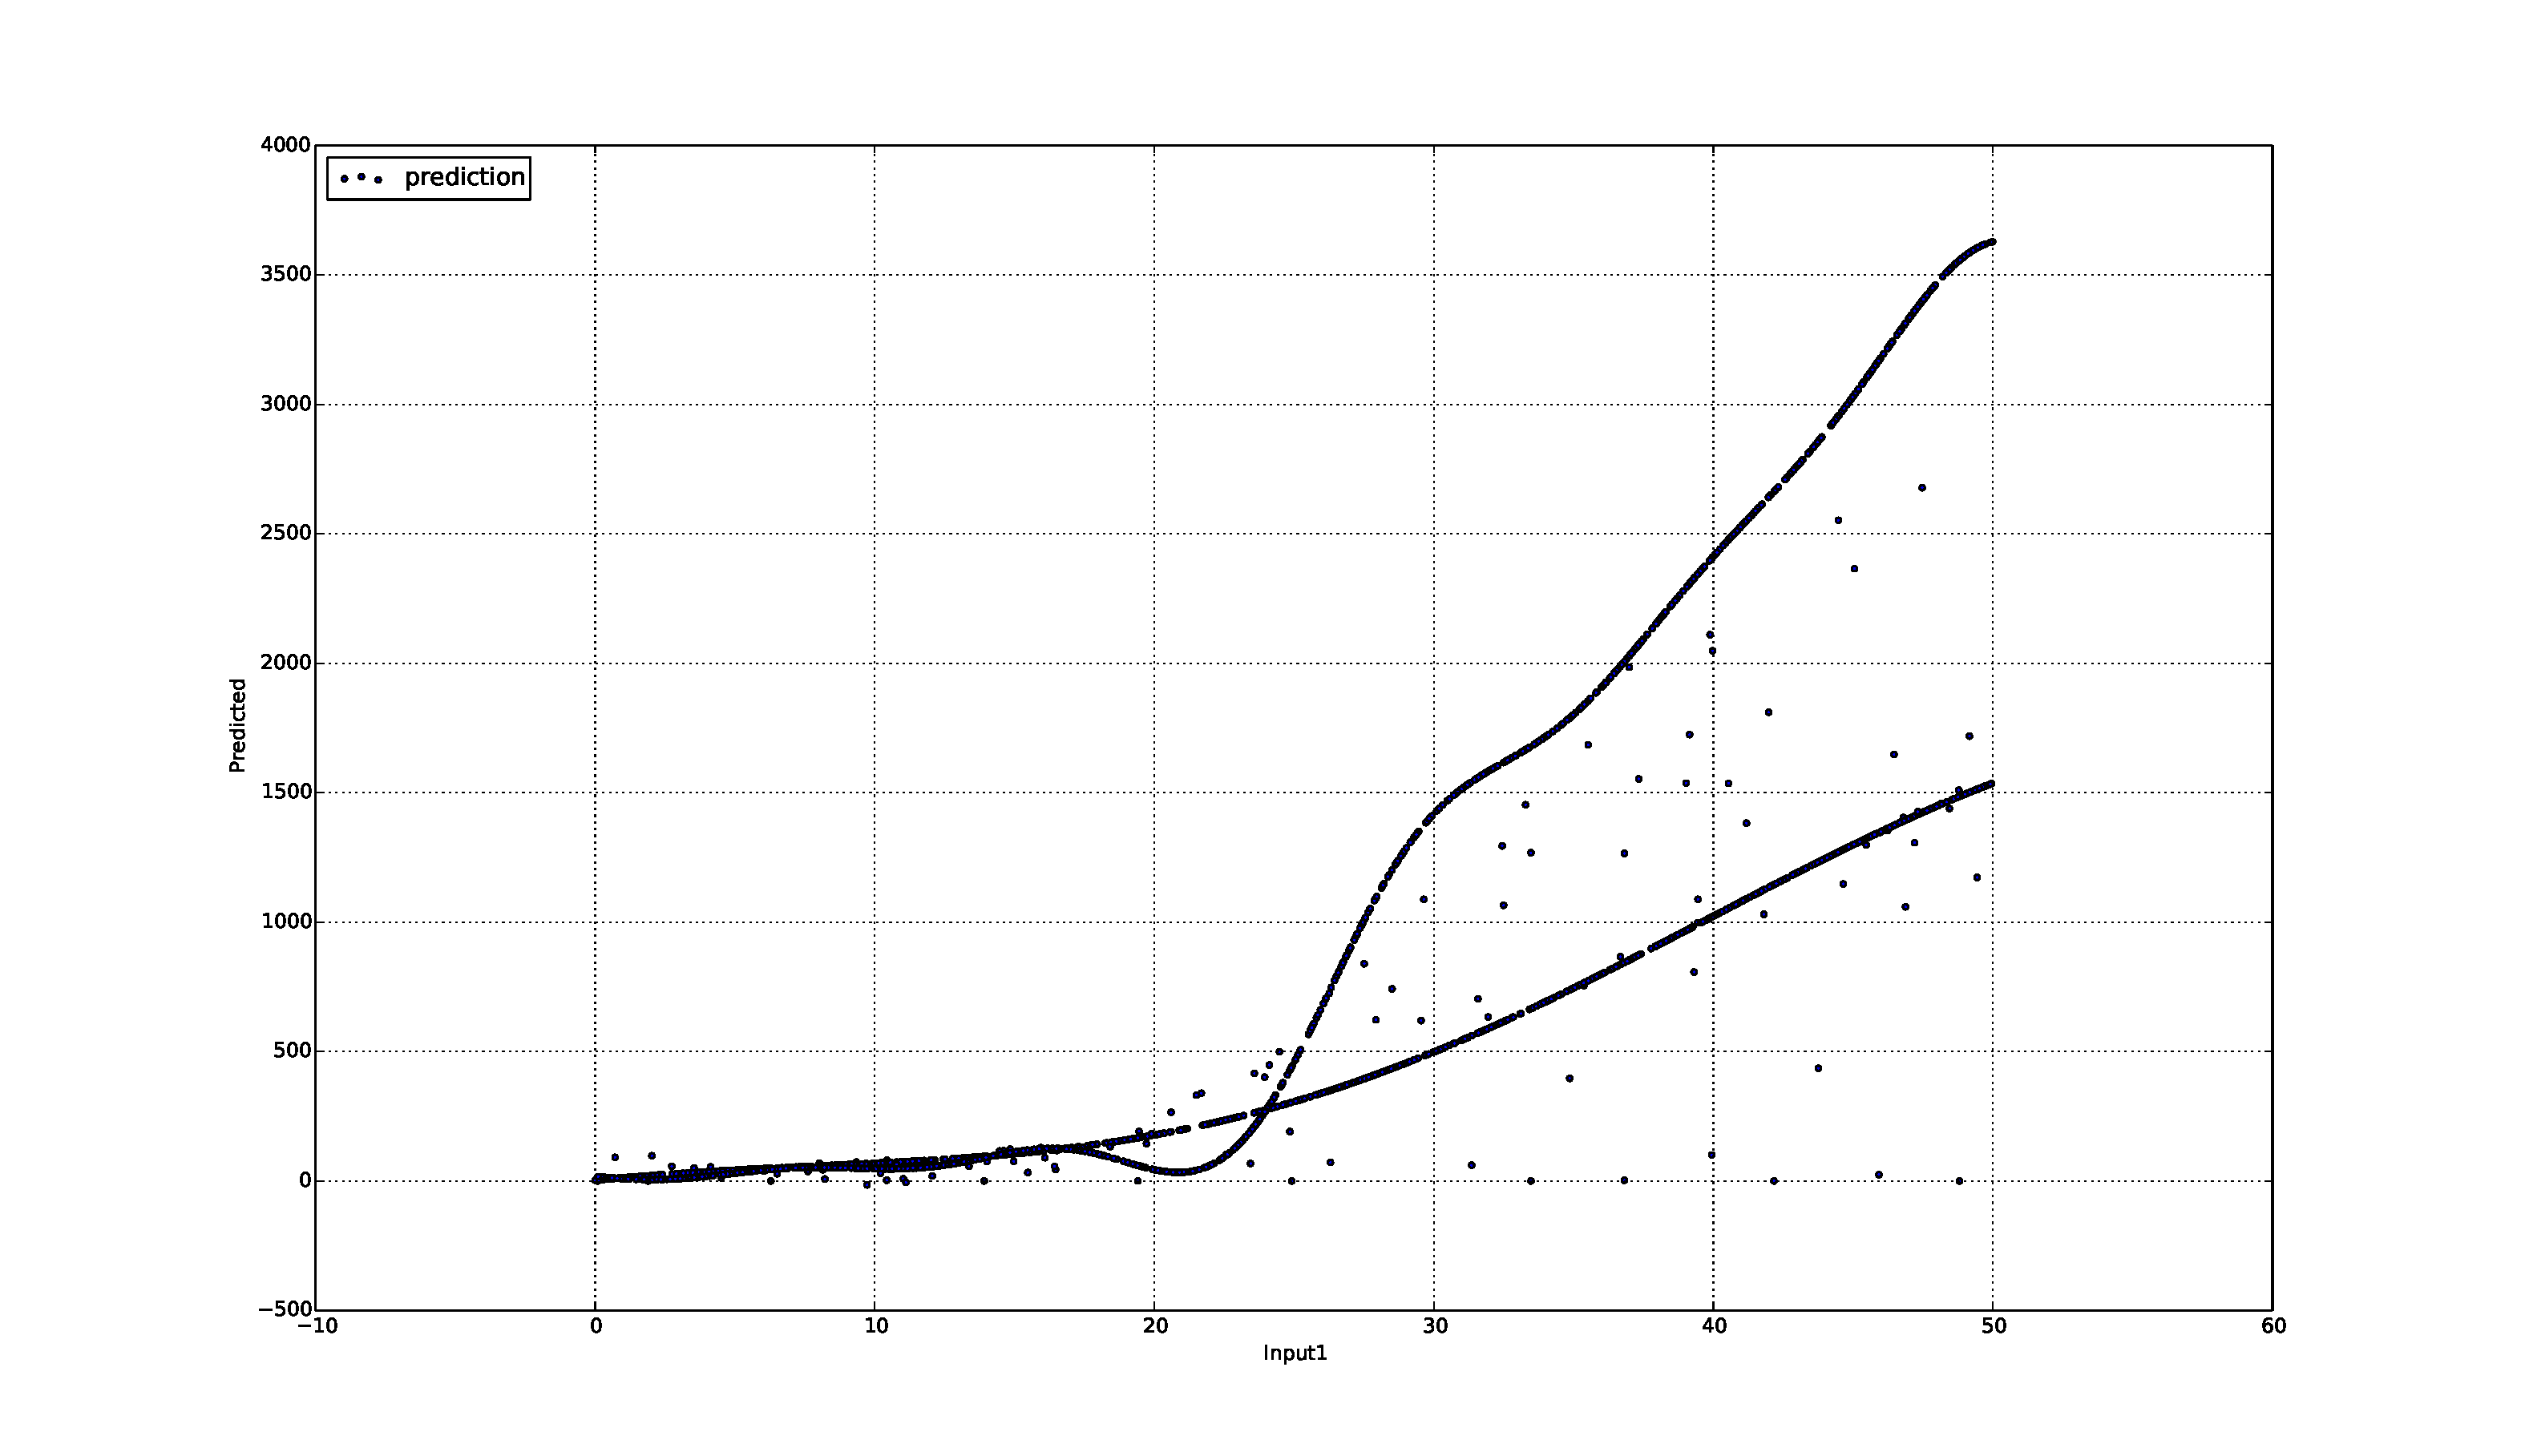
\includegraphics[width=\linewidth]{./Figures/gpreg_zeromean_ws64_approximated_func_SYNTH_D_CD_2000_1_50_1_13.pdf}
  \caption{Predictions of \texttt{GPRegressionZeroMean\_WS64} on the stream simulated from the dataset \texttt{SYNTH\_D\_CD\_2000\_1\_50\_1\_13}}
  \label{fig:gpreg_zeromean_ws64_approximated_func_SYNTH_D_CD_2000_1_50_1_13}
\end{figure}

\begin{figure}[htbp]
  \centering
    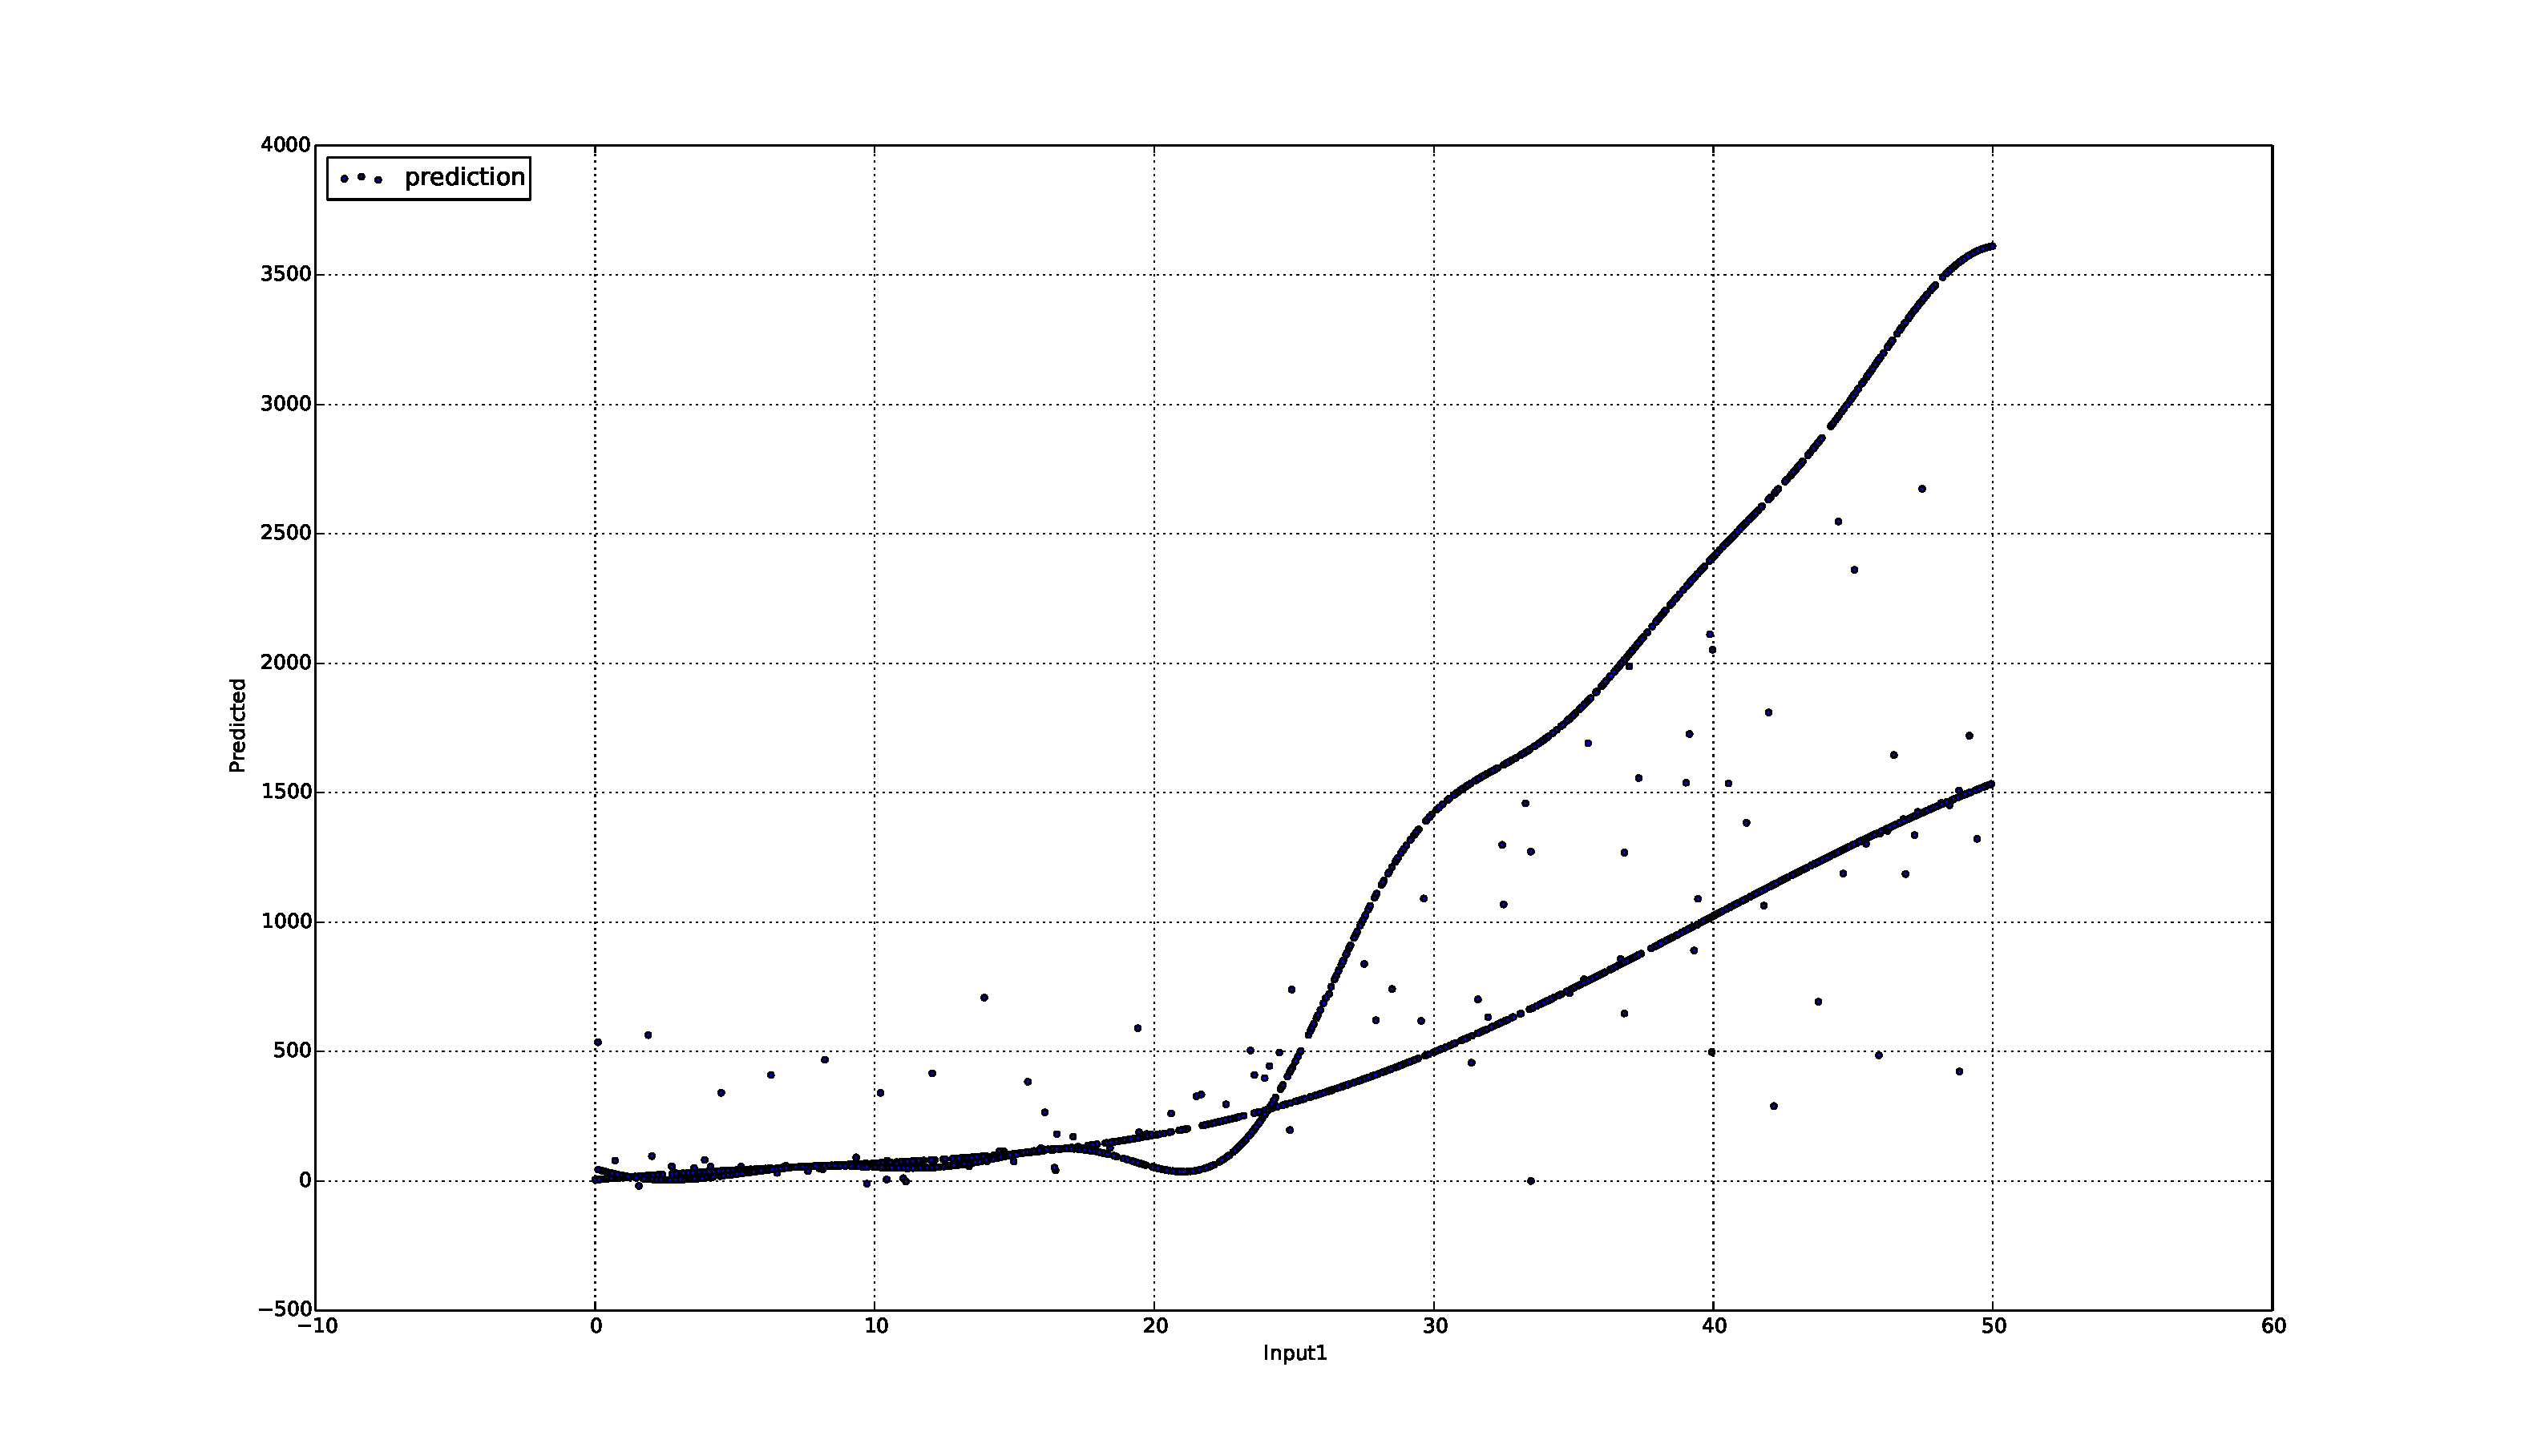
\includegraphics[width=\linewidth]{./Figures/gpreg_avgmean_ws64_approximated_func_SYNTH_D_CD_2000_1_50_1_13.pdf}
  \caption{Predictions of \texttt{GPRegressionAvgMean\_WS64} on the stream simulated from the dataset \texttt{SYNTH\_D\_CD\_2000\_1\_50\_1\_13}}
  \label{fig:gpreg_avgmean_ws64_approximated_func_SYNTH_D_CD_2000_1_50_1_13}
\end{figure}

\begin{figure}[htbp]
  \centering
    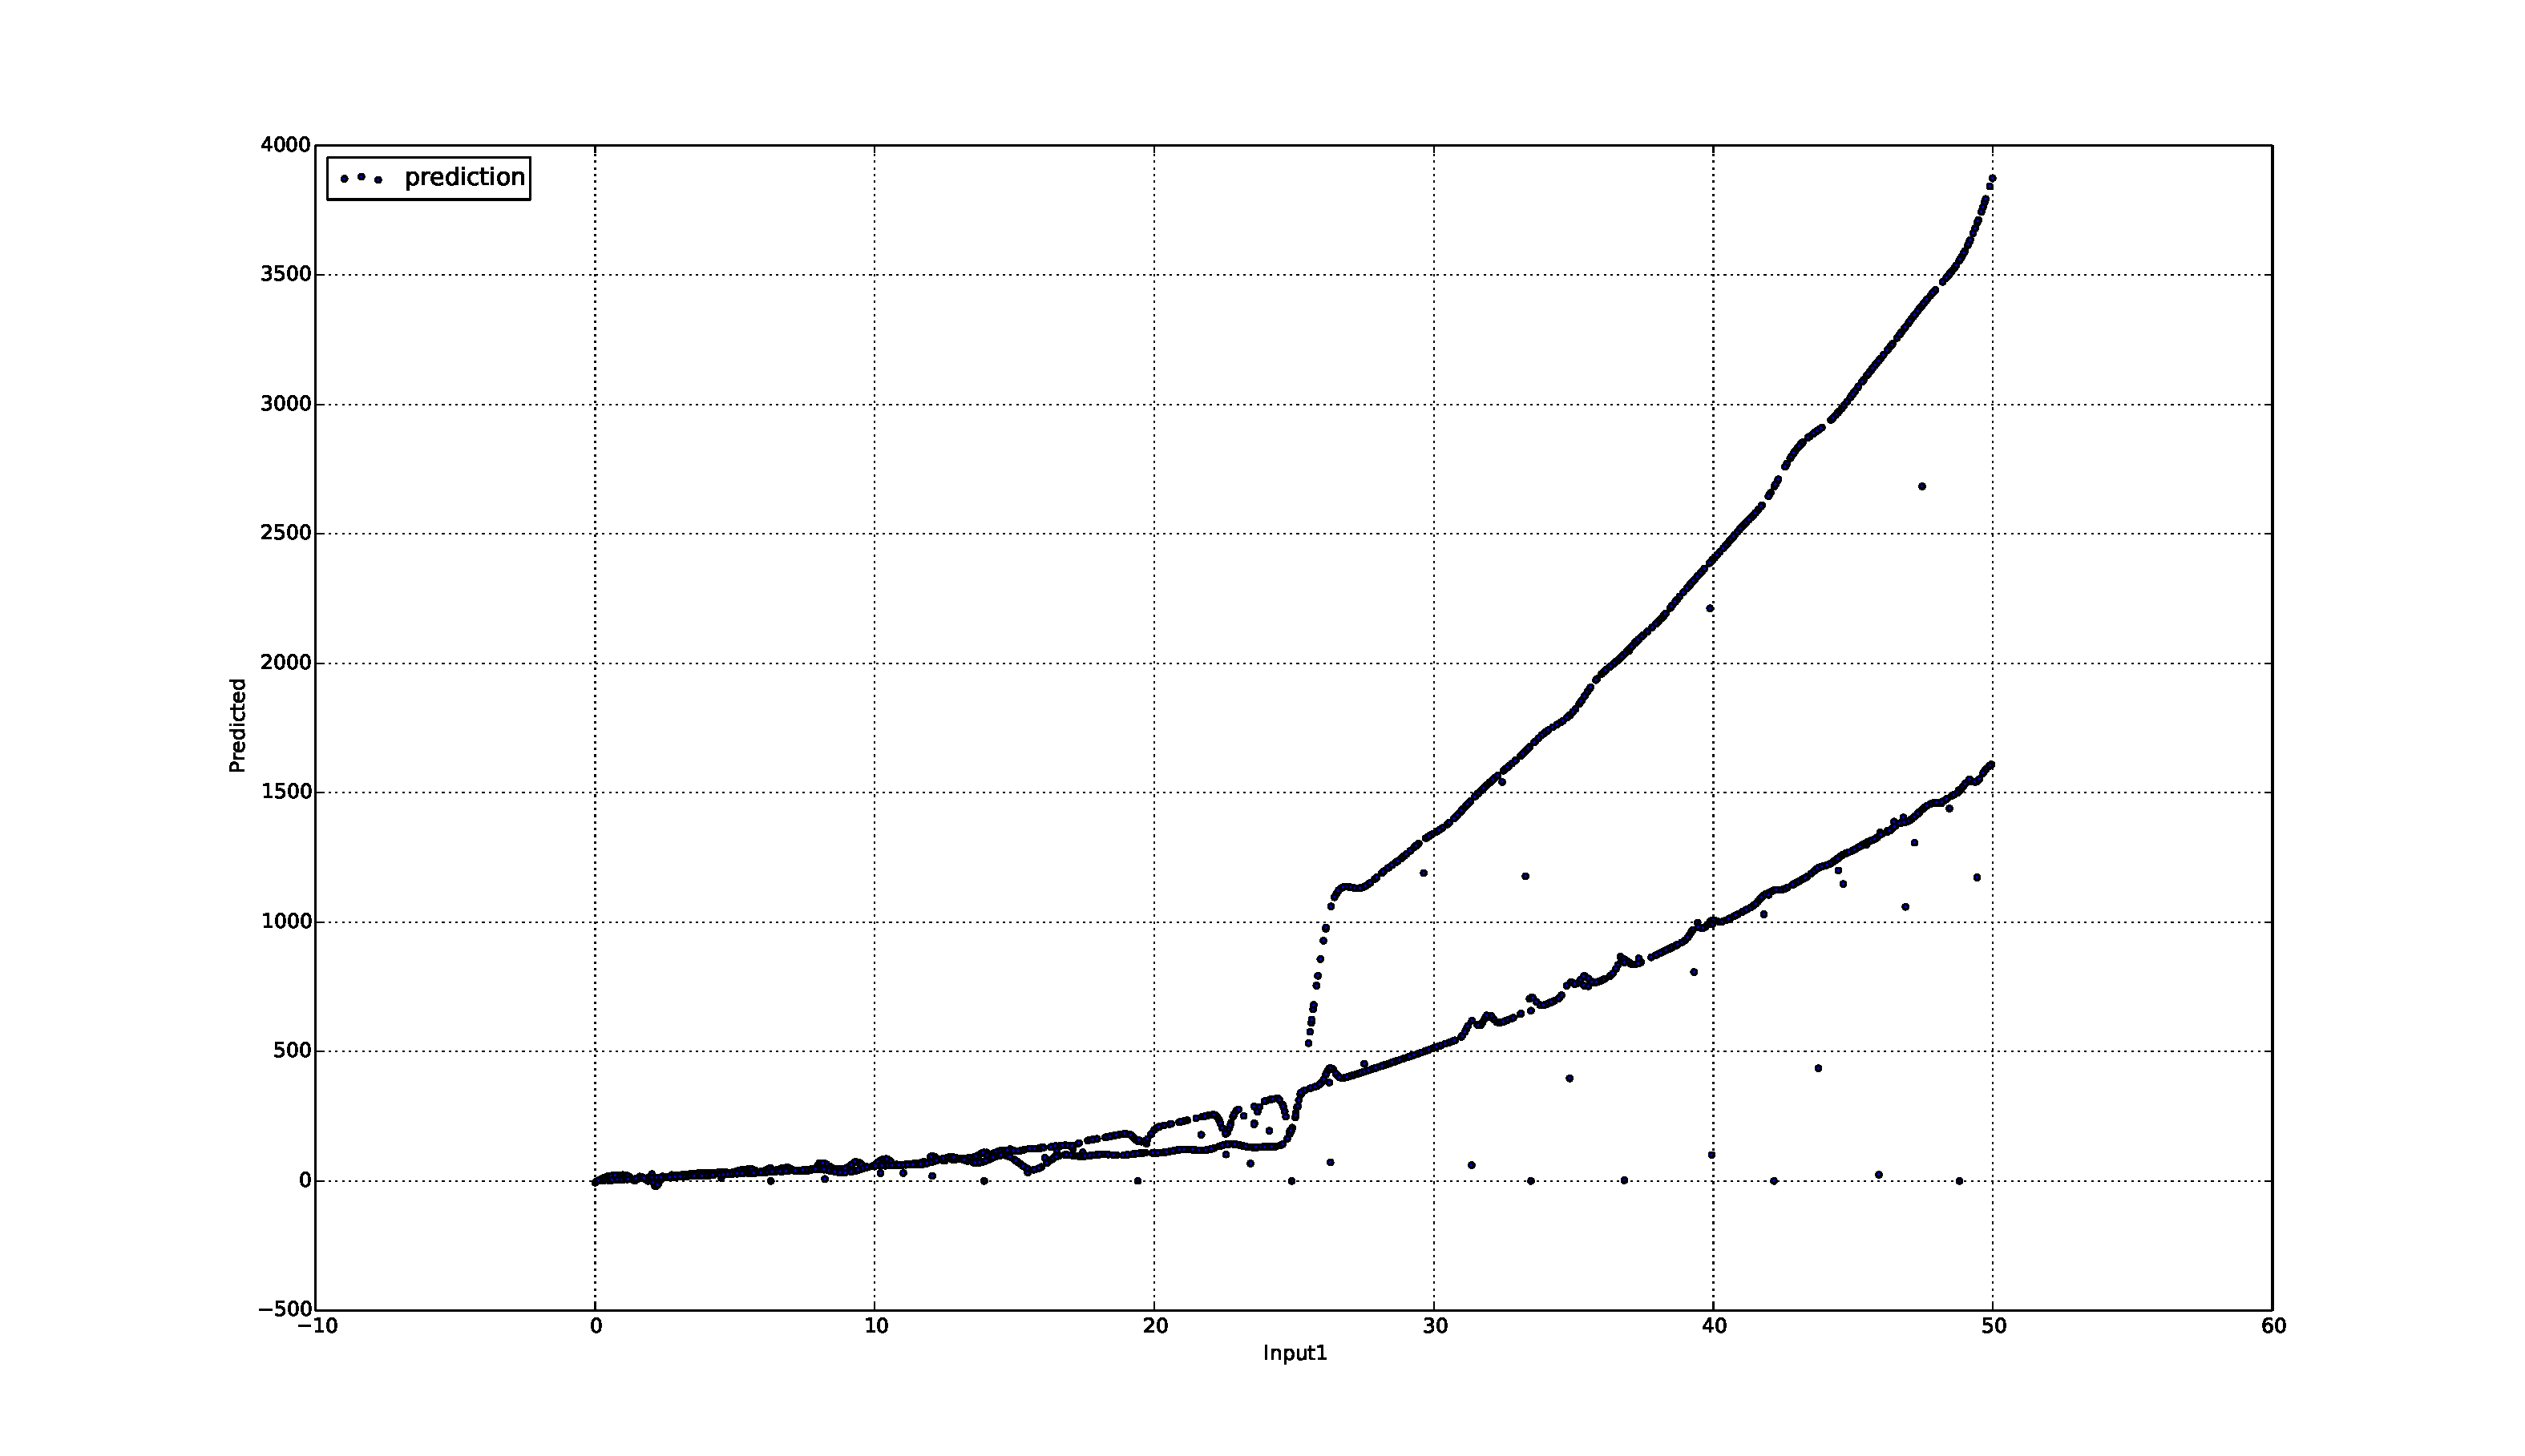
\includegraphics[width=\linewidth]{./Figures/gpreg_olsmean_ws64_approximated_func_SYNTH_D_CD_2000_1_50_1_13.pdf}
  \caption{Predictions of \texttt{GPRegressionOLSMean\_WS64} on the stream simulated from the dataset \texttt{SYNTH\_D\_CD\_2000\_1\_50\_1\_13}}
  \label{fig:gpreg_olsmean_ws64_approximated_func_SYNTH_D_CD_2000_1_50_1_13}
\end{figure}

\begin{figure}[htbp]
  \centering
    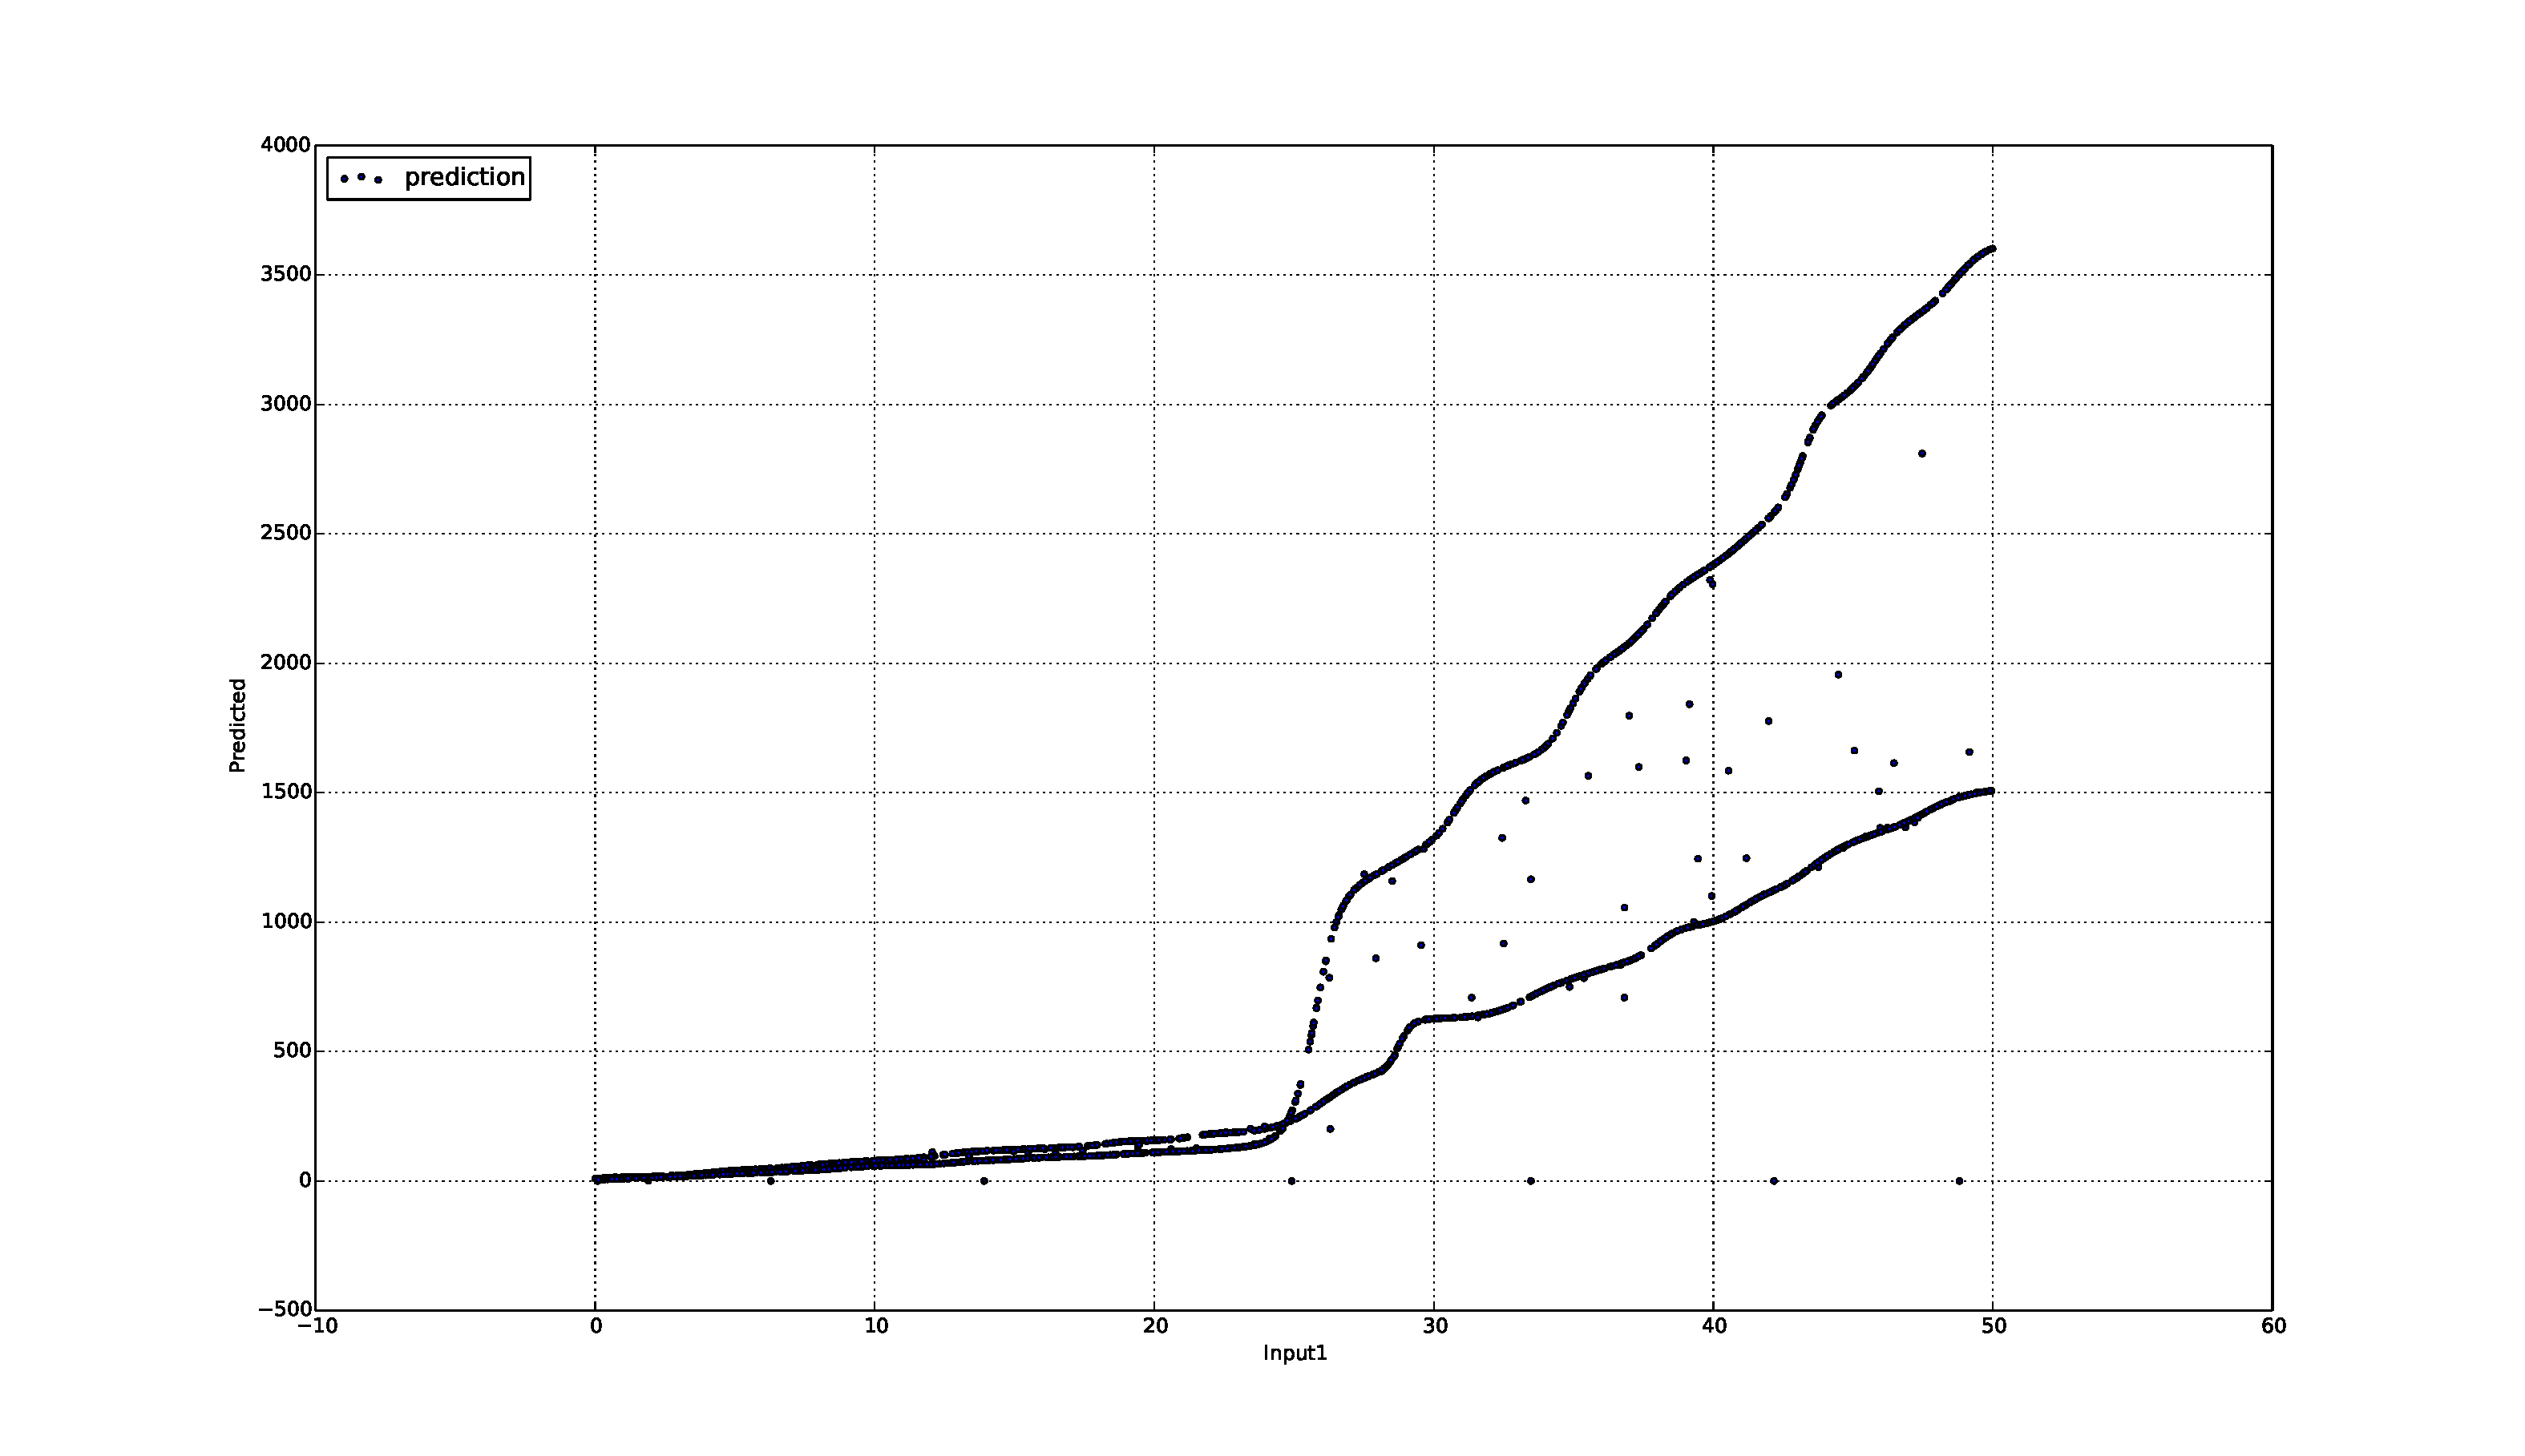
\includegraphics[width=\linewidth]{./Figures/kreg_ws64_approximated_func_SYNTH_D_CD_2000_1_50_1_13.pdf}
  \caption{Predictions of \texttt{KernelRegression\_HighConf\_WS64} on the stream simulated from the dataset \texttt{SYNTH\_D\_CD\_2000\_1\_50\_1\_13}}
  \label{fig:kreg_ws64_approximated_func_SYNTH_D_CD_2000_1_50_1_13}
\end{figure}

\begin{figure}[htbp]
  \centering
    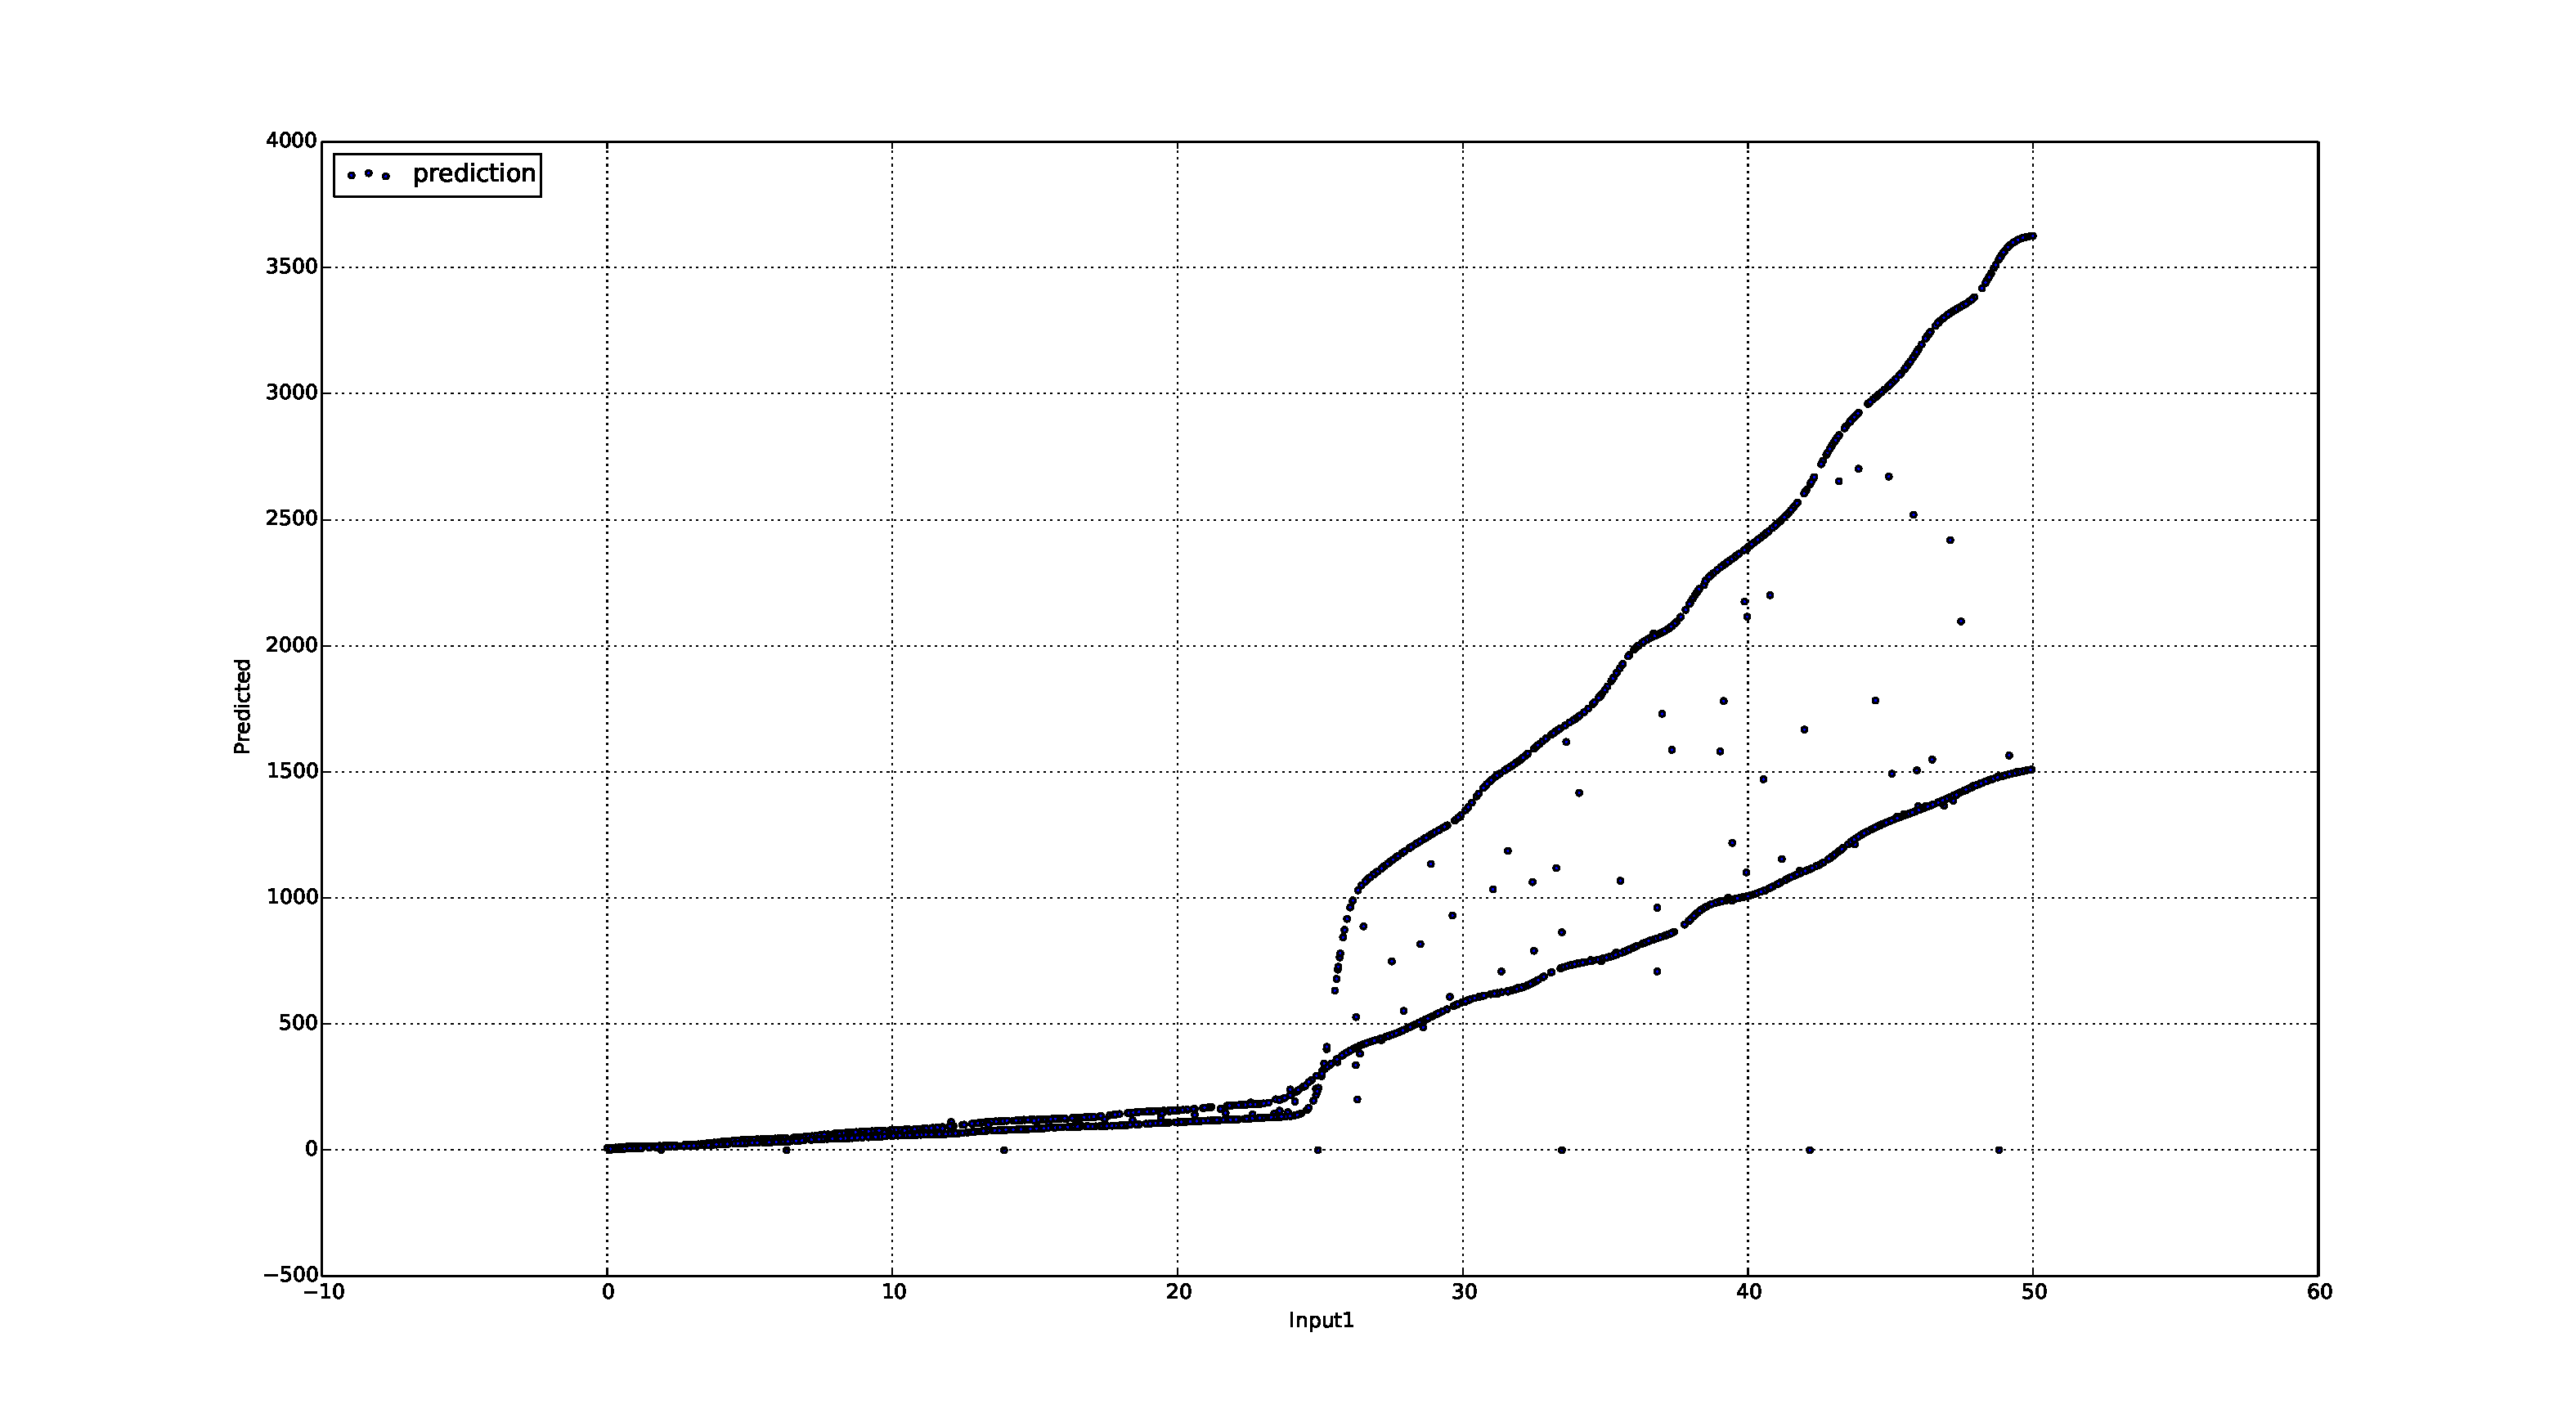
\includegraphics[width=\linewidth]{./Figures/kreg_ws96_approximated_func_SYNTH_D_CD_2000_1_50_1_13.pdf}
  \caption{Predictions of \texttt{KernelRegression\_HighConf\_WS96} on the stream simulated from the dataset \texttt{SYNTH\_D\_CD\_2000\_1\_50\_1\_13}}
  \label{fig:kreg_ws96_approximated_func_SYNTH_D_CD_2000_1_50_1_13}
\end{figure}

\begin{figure}[htbp]
  \centering
    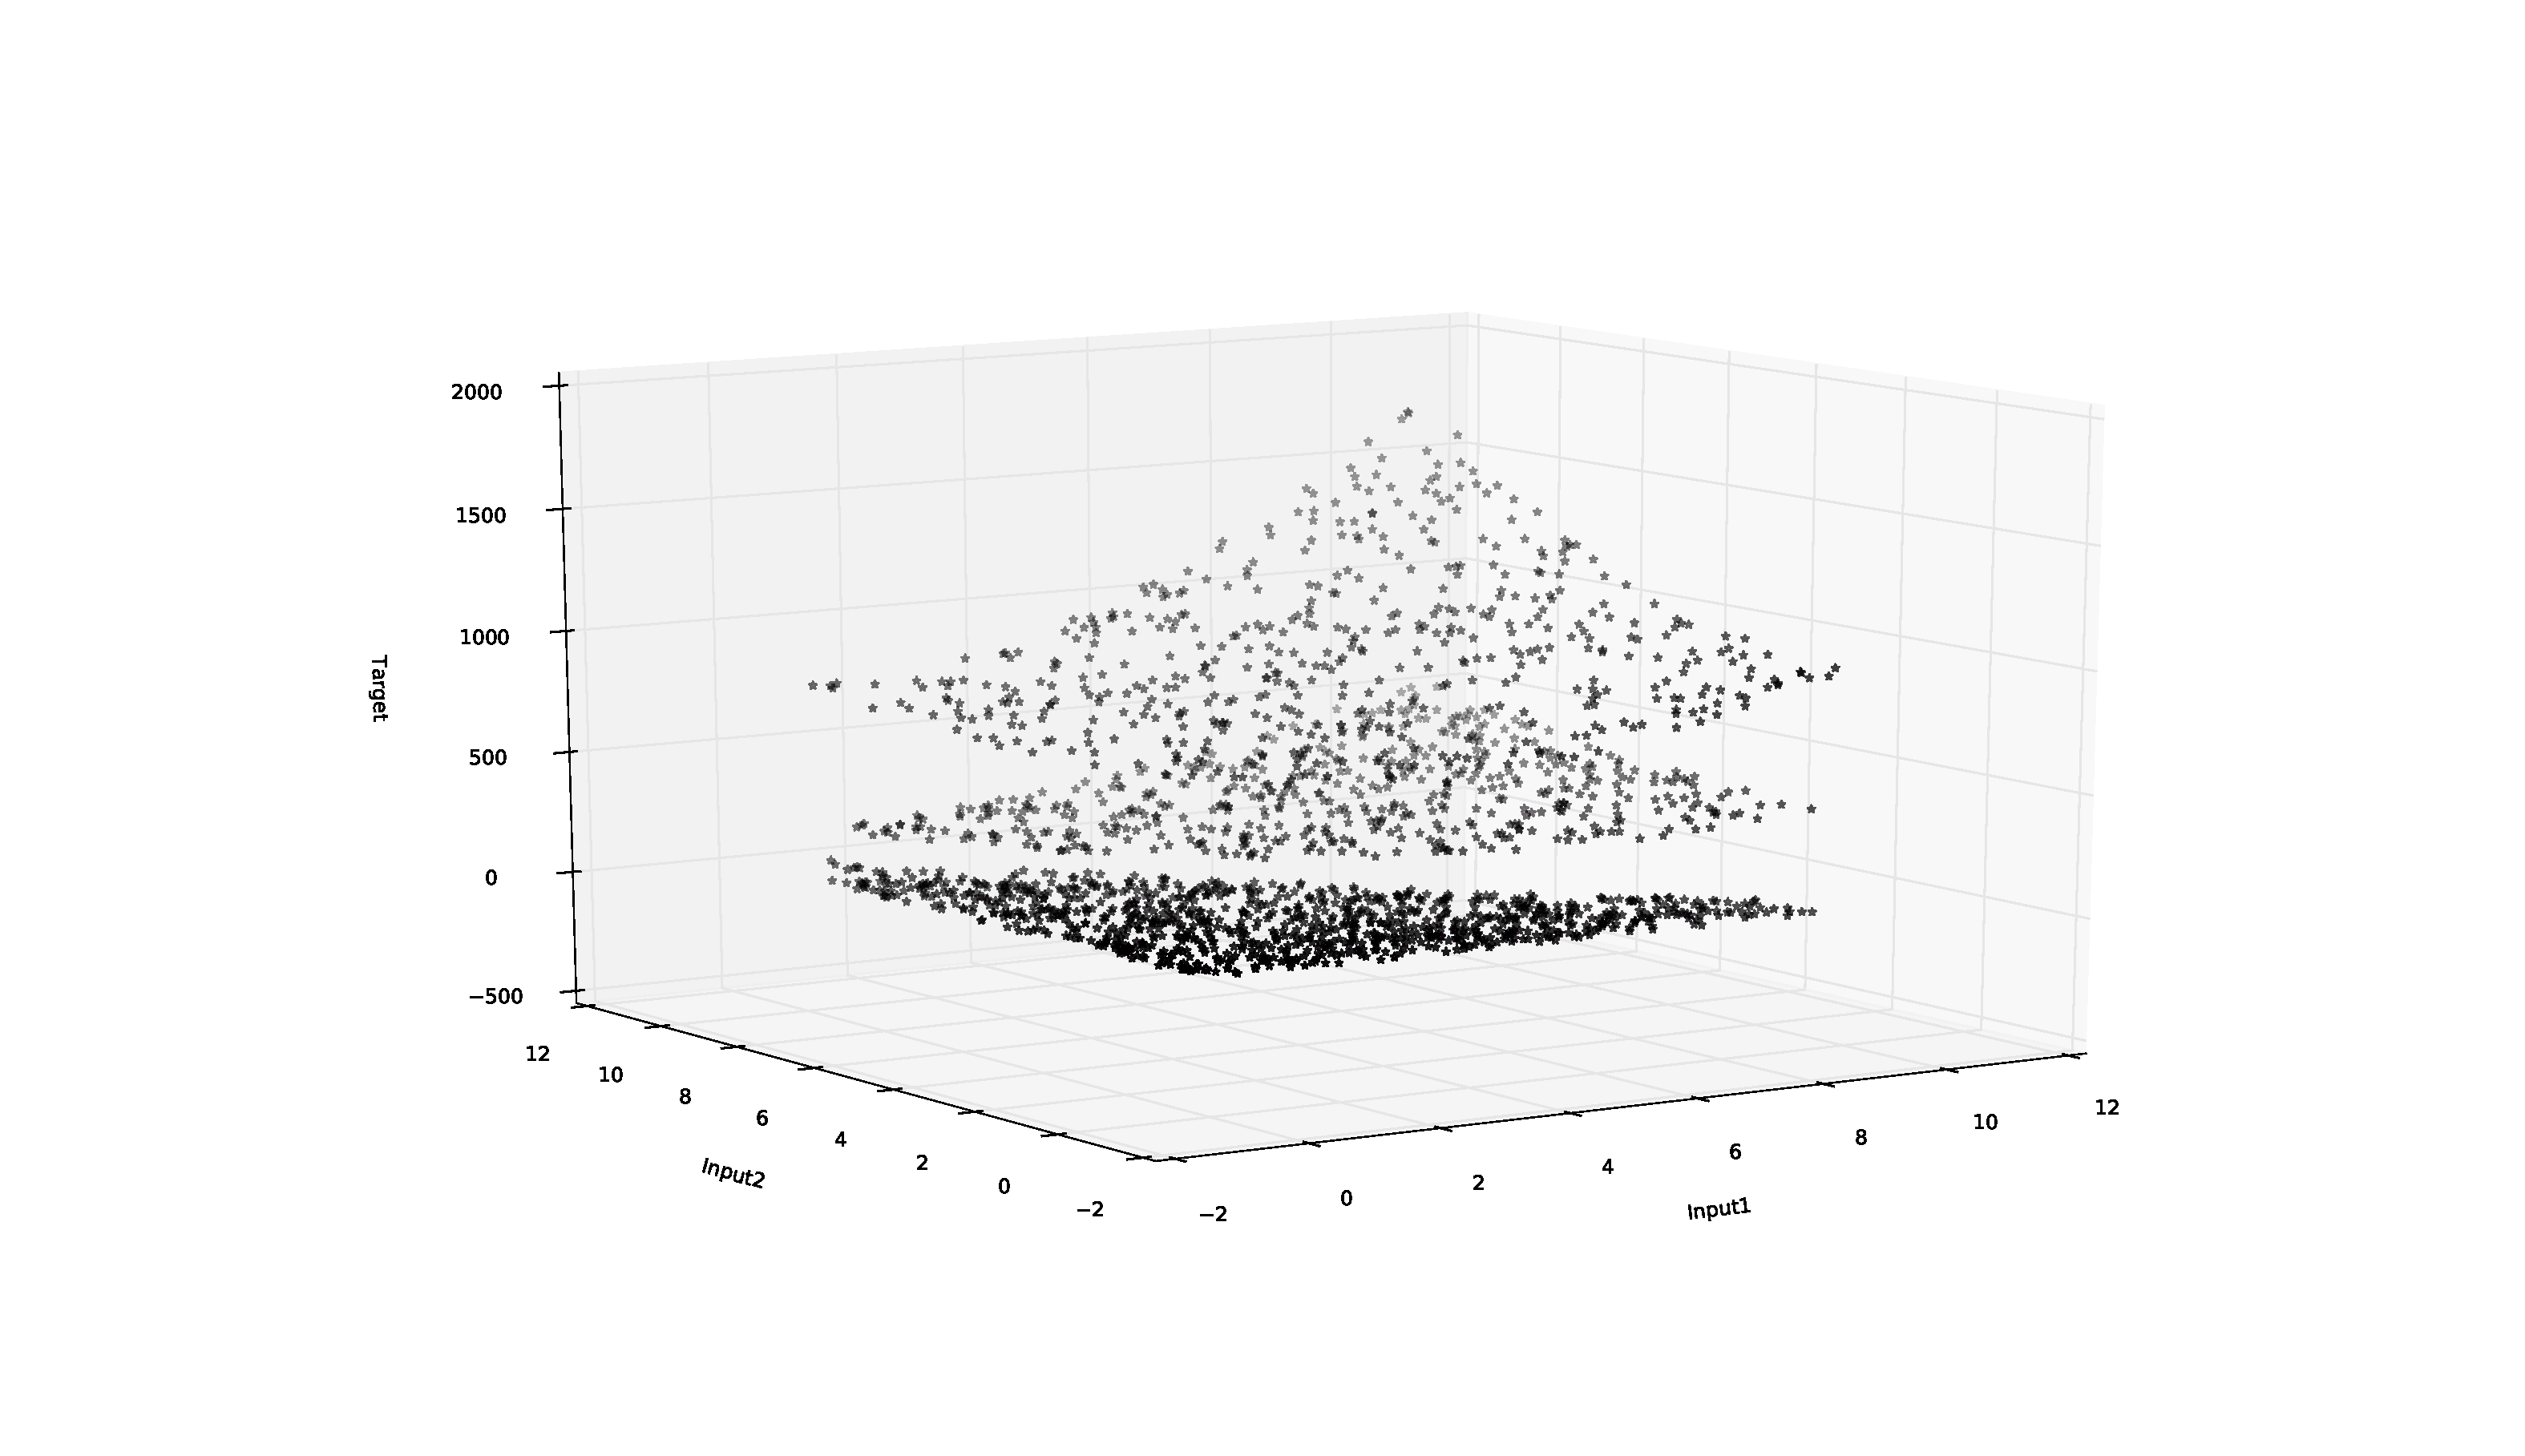
\includegraphics[width=\linewidth]{./Figures/ref_func_SYNTH_D_CD_2000_2_10_1_13.pdf}
  \caption{Visualization of the stream simulated from dataset} \texttt{SYNTH\_D\_CD\_2000\_2\_10\_1\_13}
  \label{fig:ref_func_SYNTH_D_CD_2000_2_10_1_13}
\end{figure}

\begin{figure}[htbp]
  \centering
    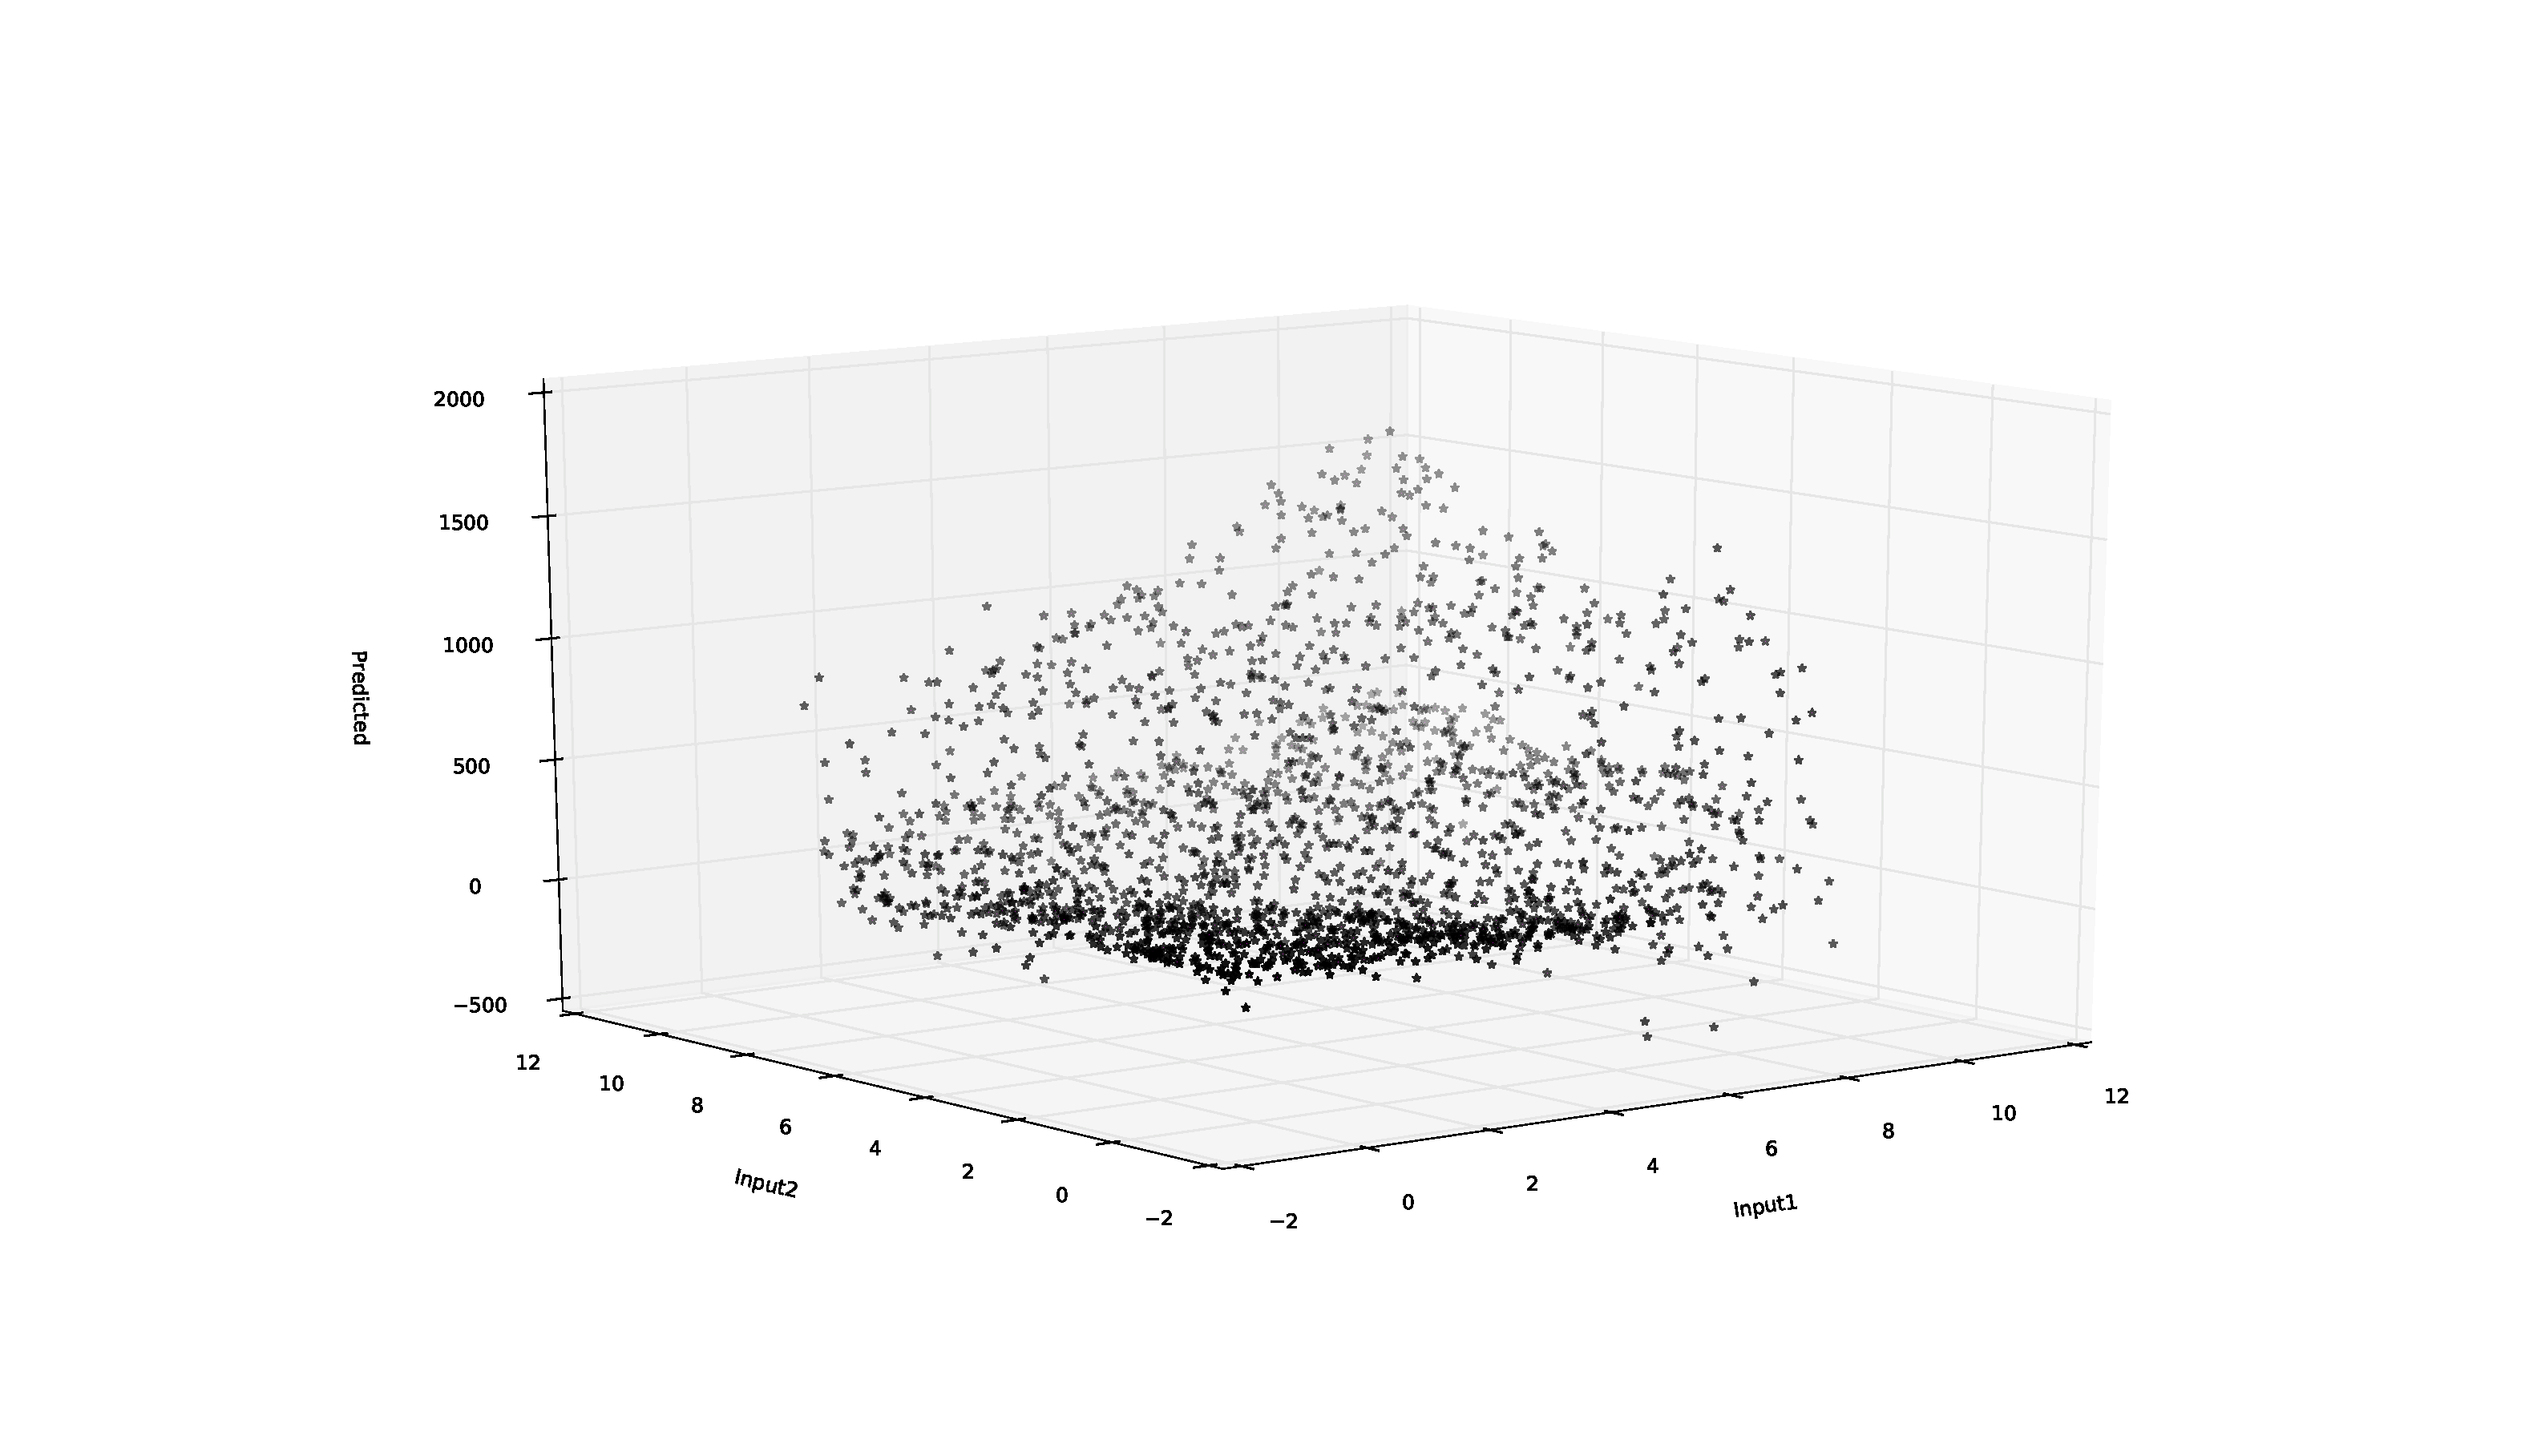
\includegraphics[width=\linewidth]{./Figures/gpreg_zeromean_ws64_approximated_func_SYNTH_D_CD_2000_2_10_1_13.pdf}
  \caption{Predictions of \texttt{GPRegressionZeroMean\_WS64} on the stream simulated from the dataset \texttt{SYNTH\_D\_CD\_2000\_2\_10\_1\_13}}
  \label{fig:gpreg_zeromean_ws64_approximated_func_SYNTH_D_CD_2000_2_10_1_13}
\end{figure}

\begin{figure}[htbp]
  \centering
    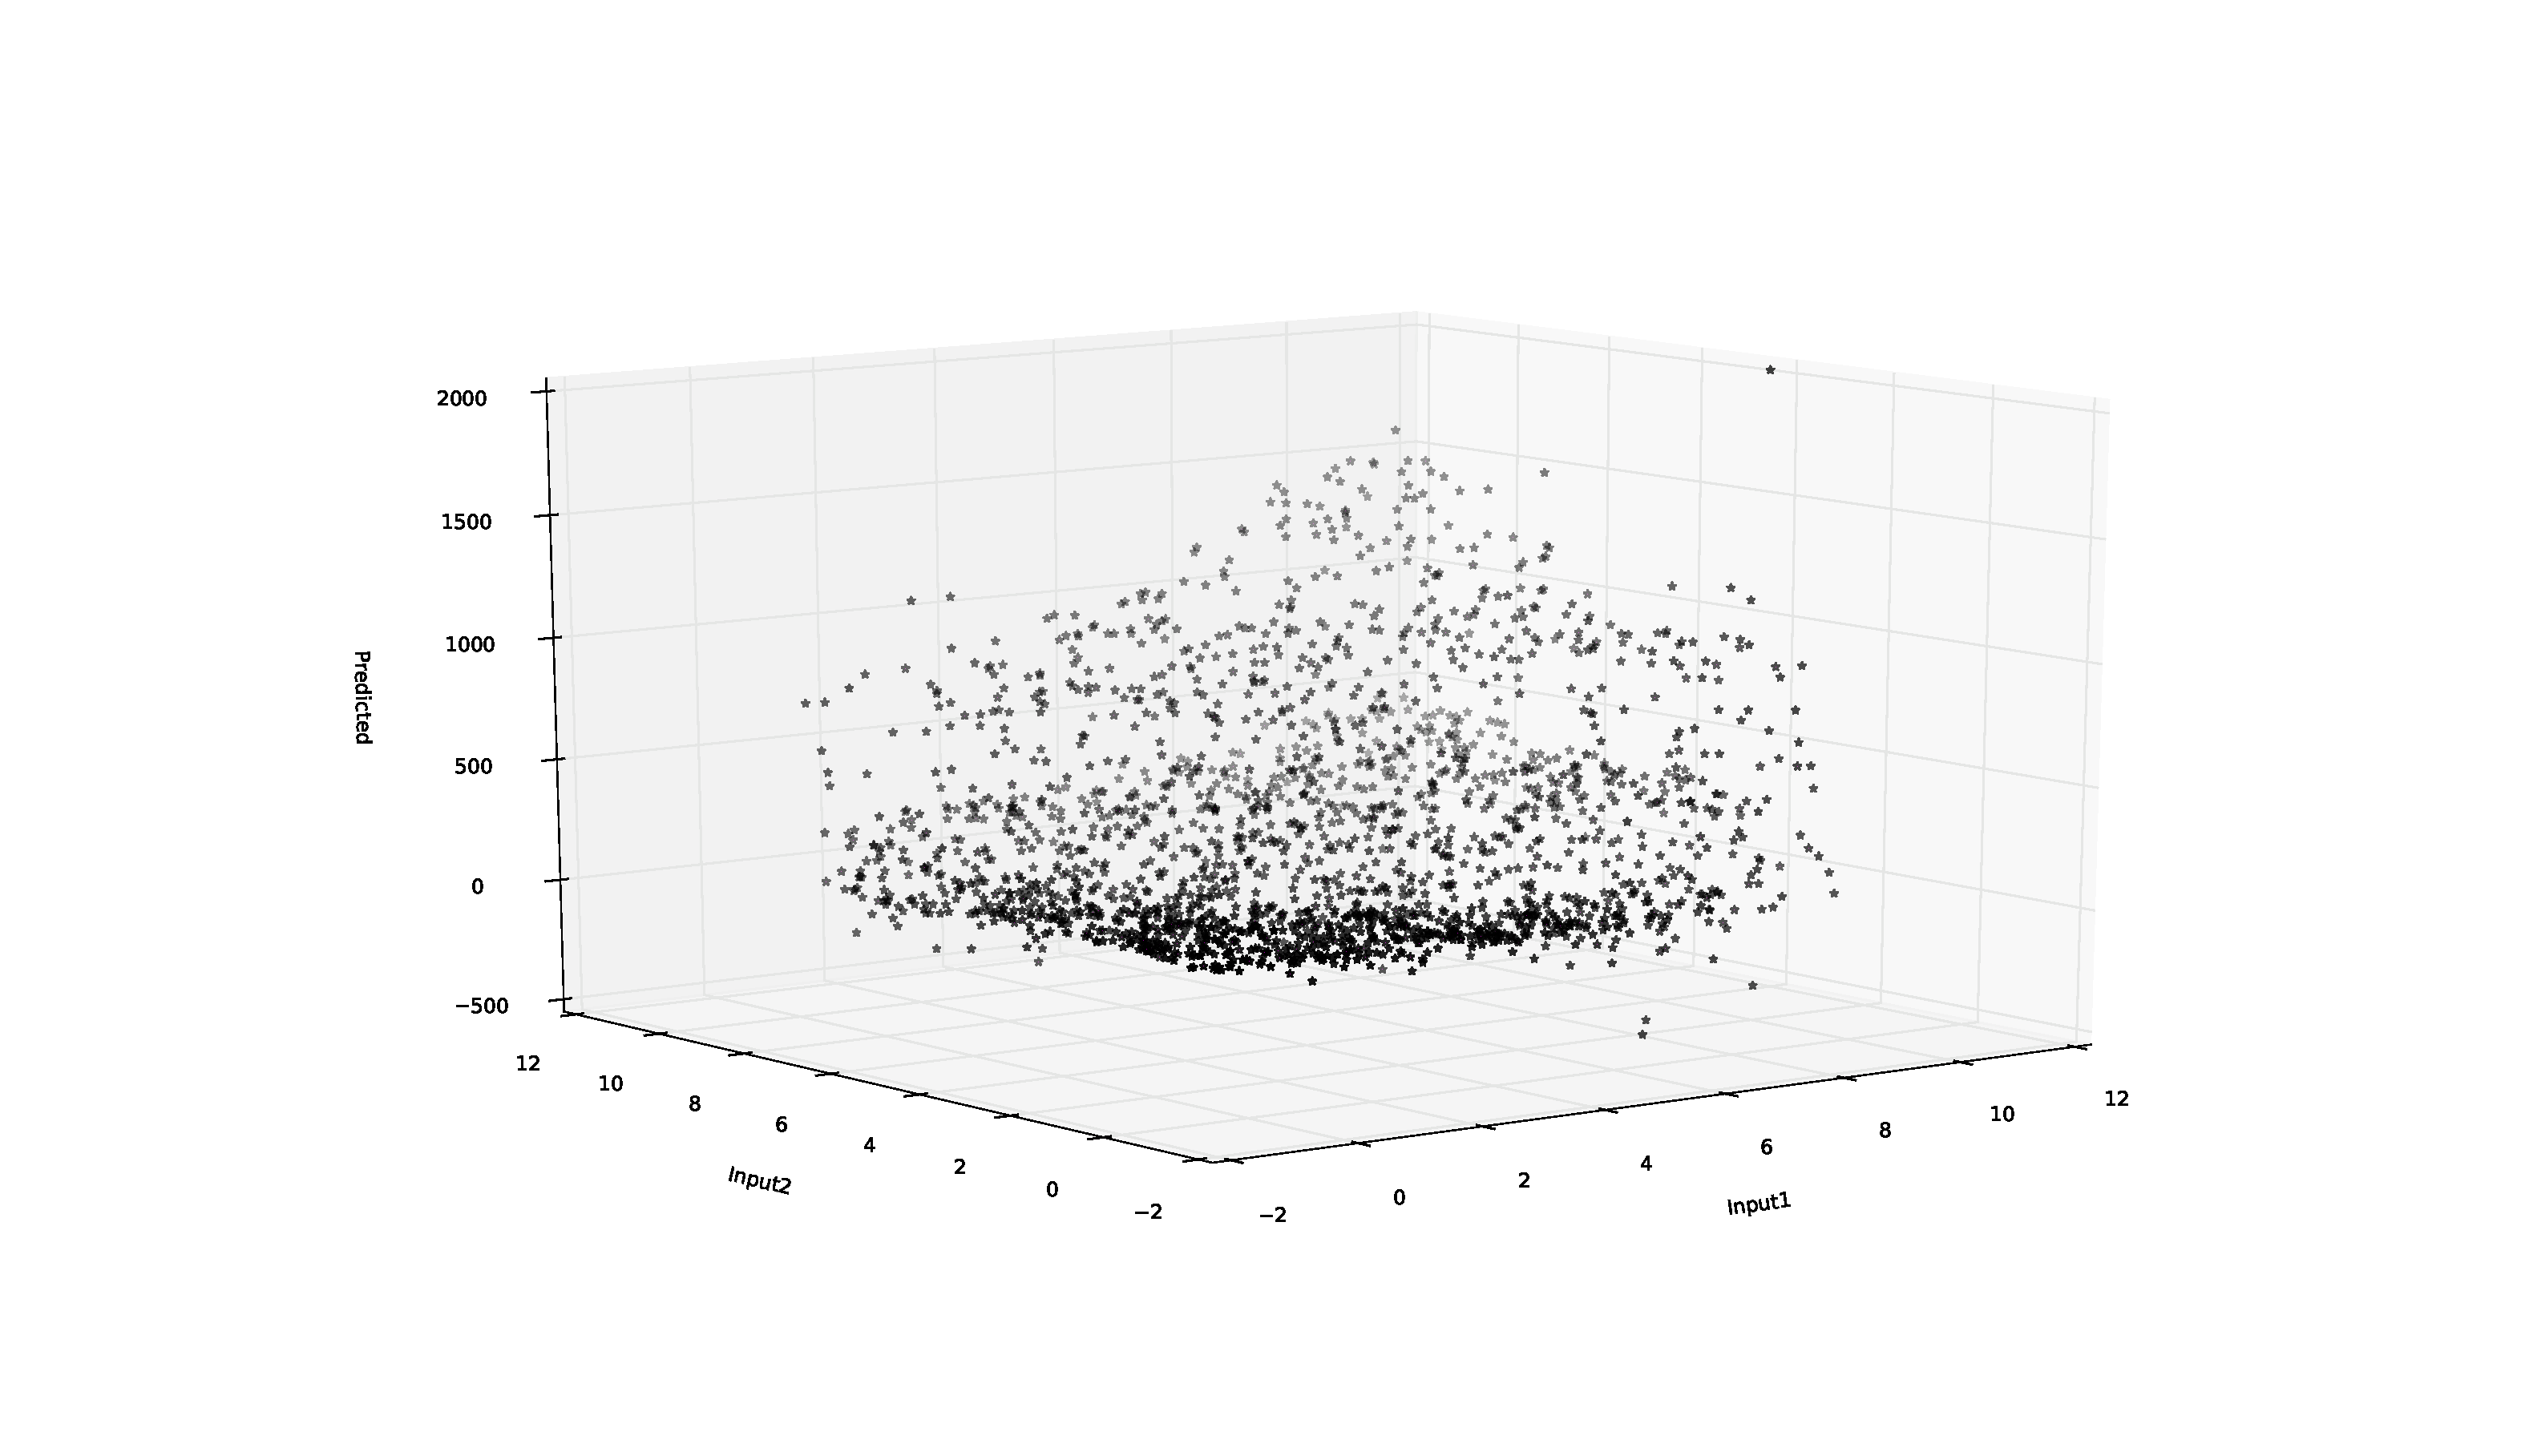
\includegraphics[width=\linewidth]{./Figures/gpreg_avgmean_ws64_approximated_func_SYNTH_D_CD_2000_2_10_1_13.pdf}
  \caption{Predictions of \texttt{GPRegressionAvgMean\_WS64} on the stream simulated from the dataset \texttt{SYNTH\_D\_CD\_2000\_2\_10\_1\_13}}
  \label{fig:gpreg_avgmean_ws64_approximated_func_SYNTH_D_CD_2000_2_10_1_13}
\end{figure}

\begin{figure}[htbp]
  \centering
    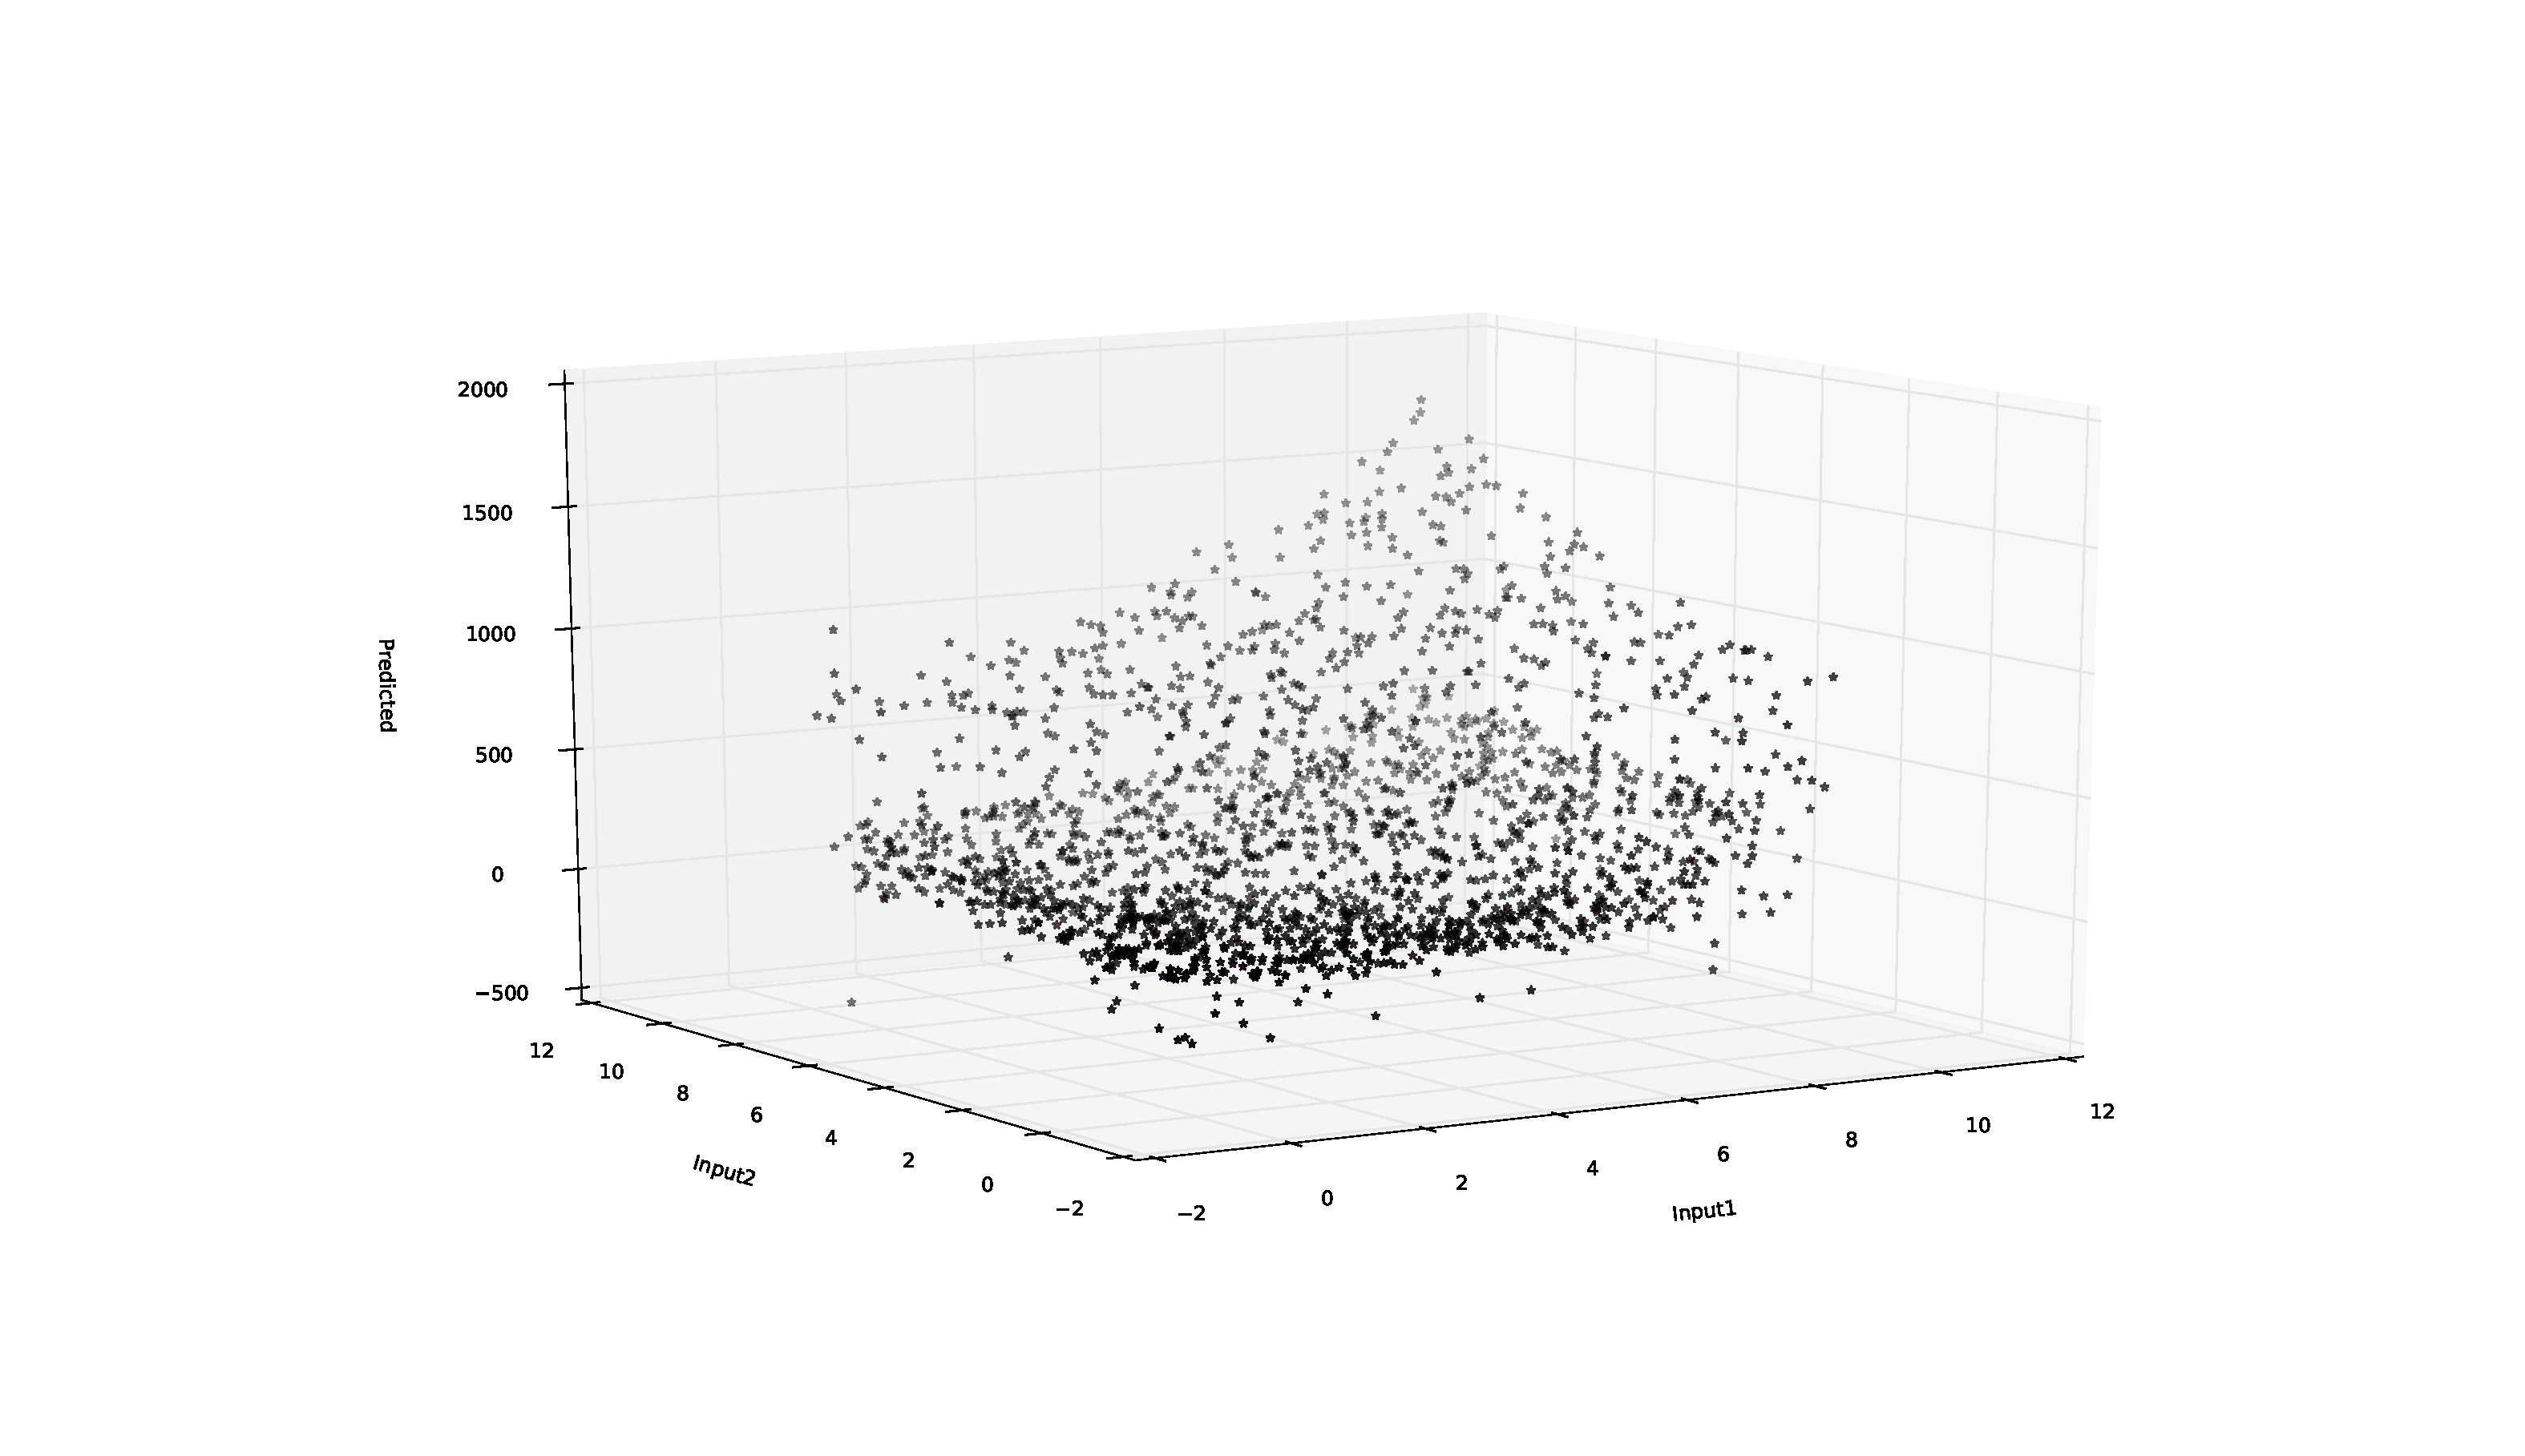
\includegraphics[width=\linewidth]{./Figures/gpreg_olsmean_ws64_approximated_func_SYNTH_D_CD_2000_2_10_1_13.pdf}
  \caption{Predictions of \texttt{GPRegressionOLSMean\_WS64} on the stream simulated from the dataset \texttt{SYNTH\_D\_CD\_2000\_2\_10\_1\_13}}
  \label{fig:gpreg_olsmean_ws64_approximated_func_SYNTH_D_CD_2000_2_10_1_13}
\end{figure}

\begin{figure}[htbp]
  \centering
    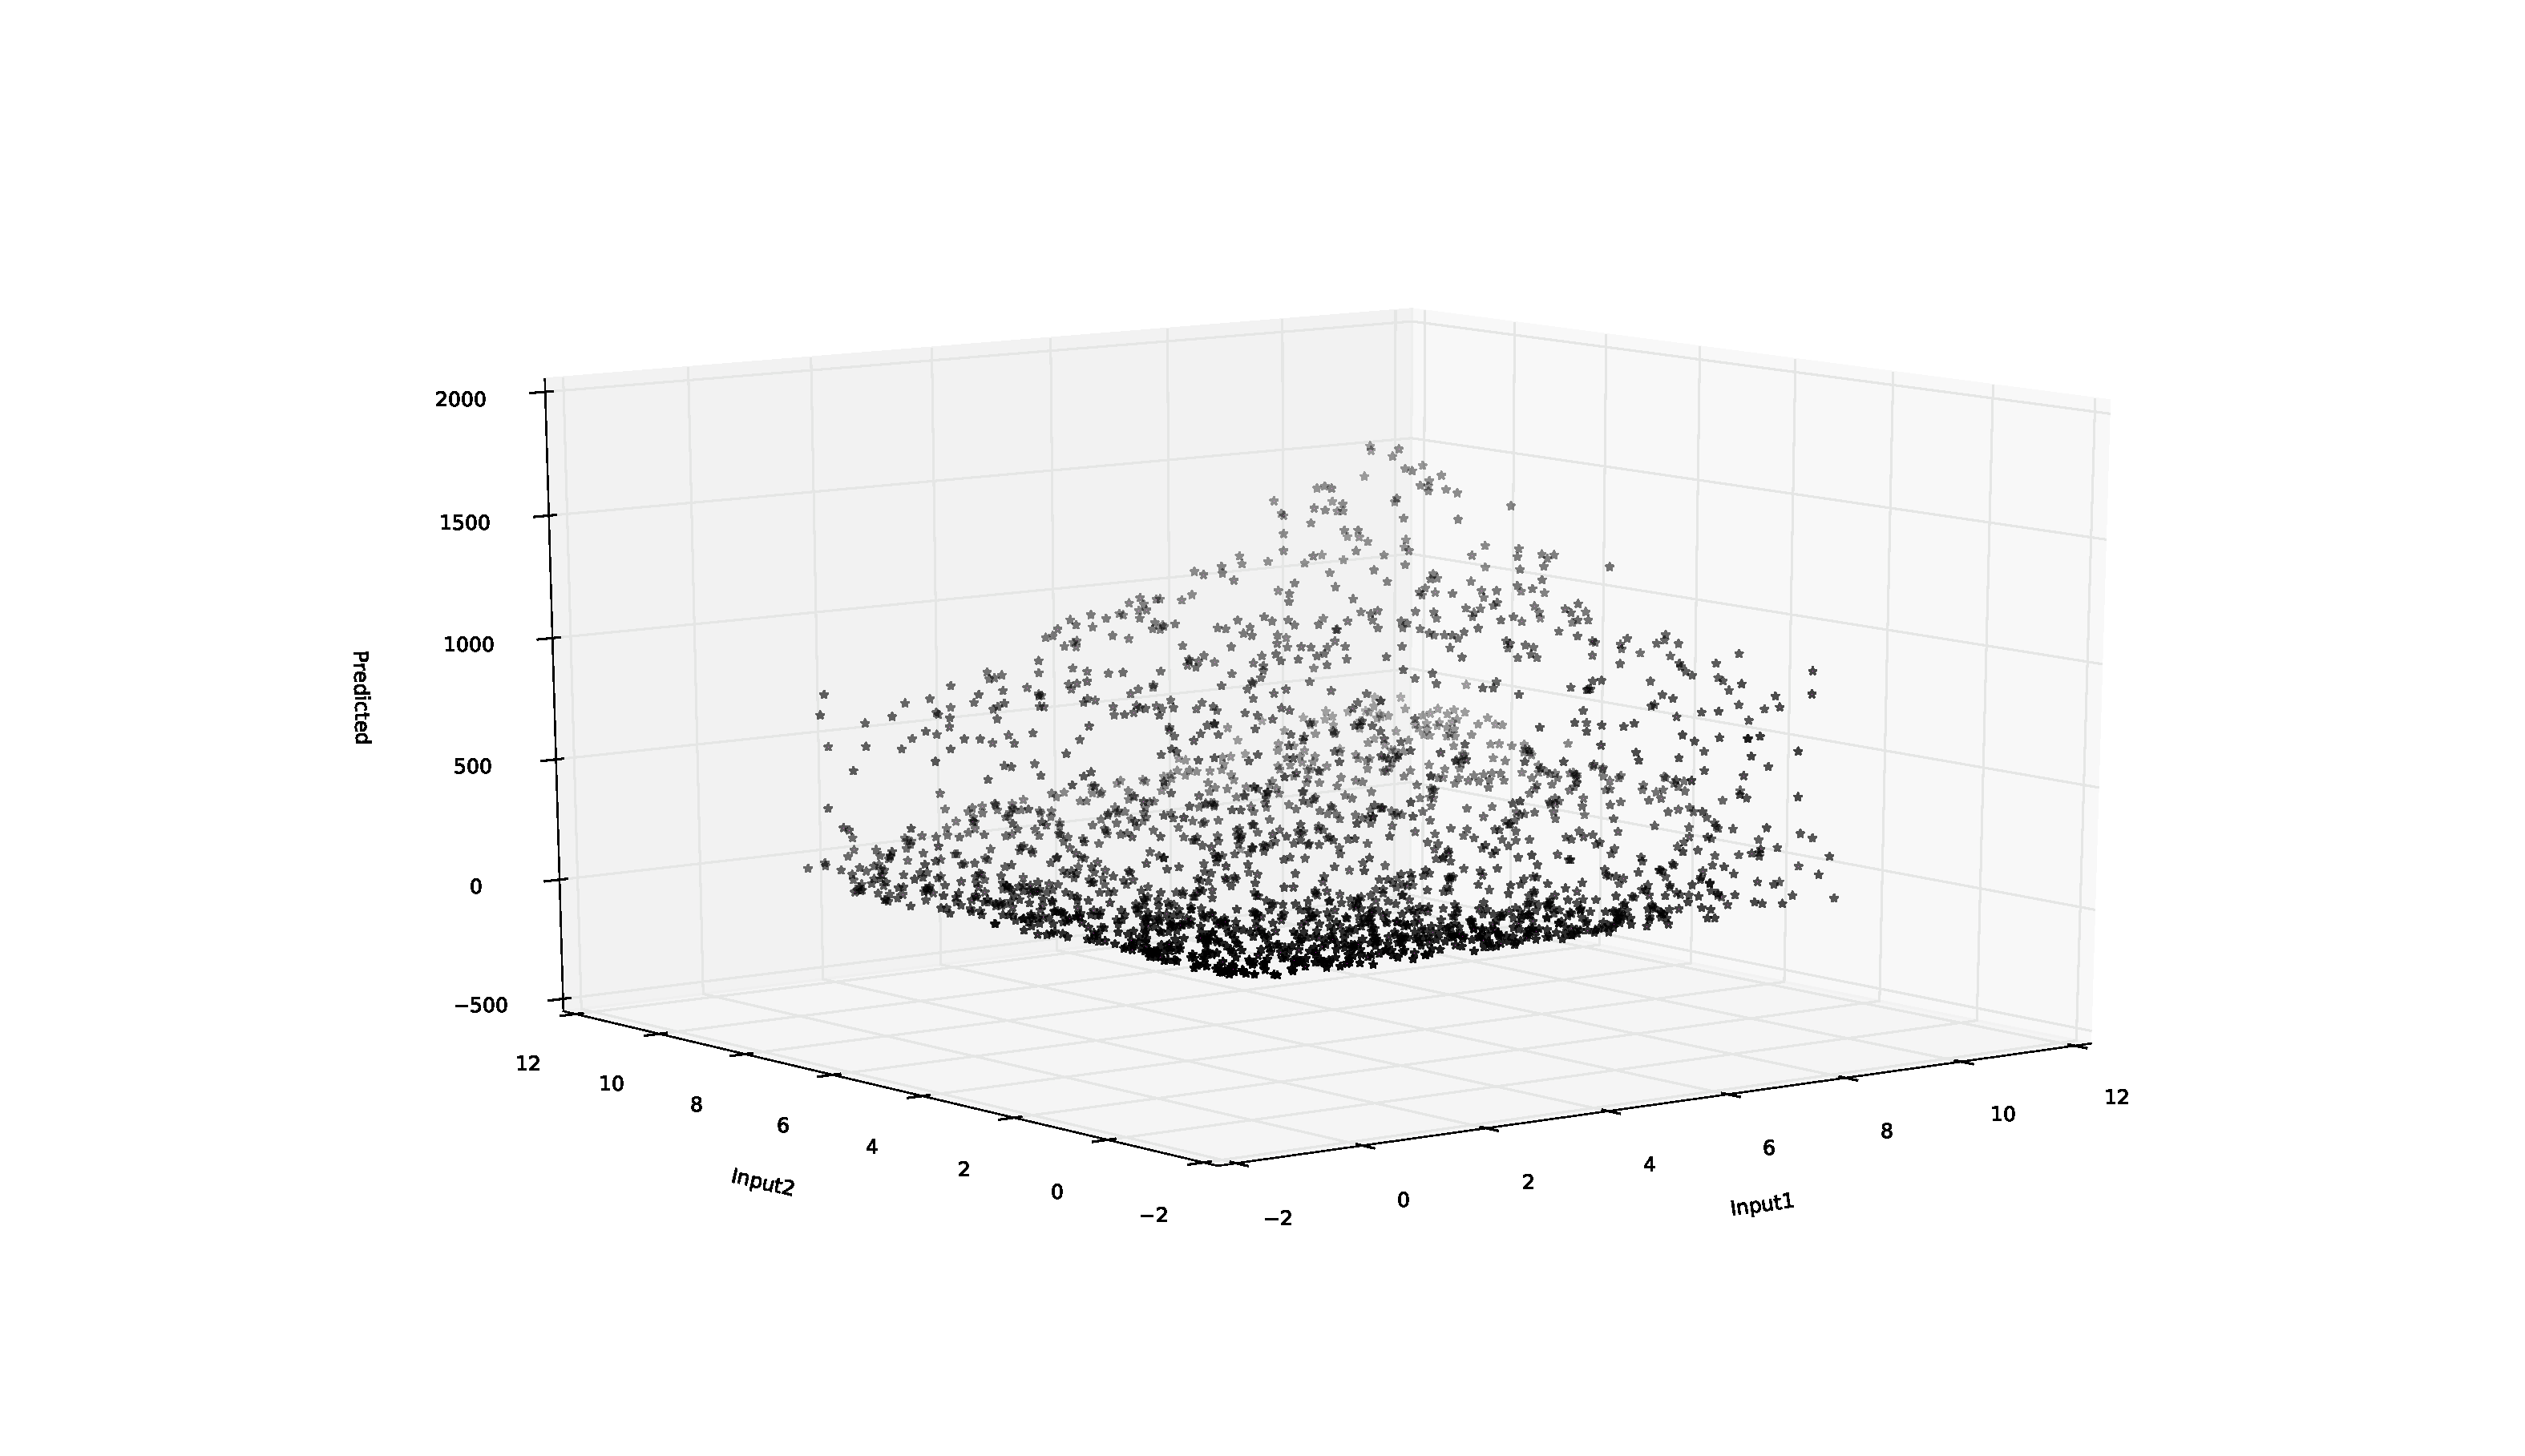
\includegraphics[width=\linewidth]{./Figures/kreg_ws64_approximated_func_SYNTH_D_CD_2000_2_10_1_13.pdf}
  \caption{Predictions of \texttt{KernelRegression\_HighConf\_WS64} on the stream simulated from the dataset \texttt{SYNTH\_D\_CD\_2000\_2\_10\_1\_13}}
  \label{fig:kreg_ws64_approximated_func_SYNTH_D_CD_2000_2_10_1_13}
\end{figure}

\begin{figure}[htbp]
  \centering
    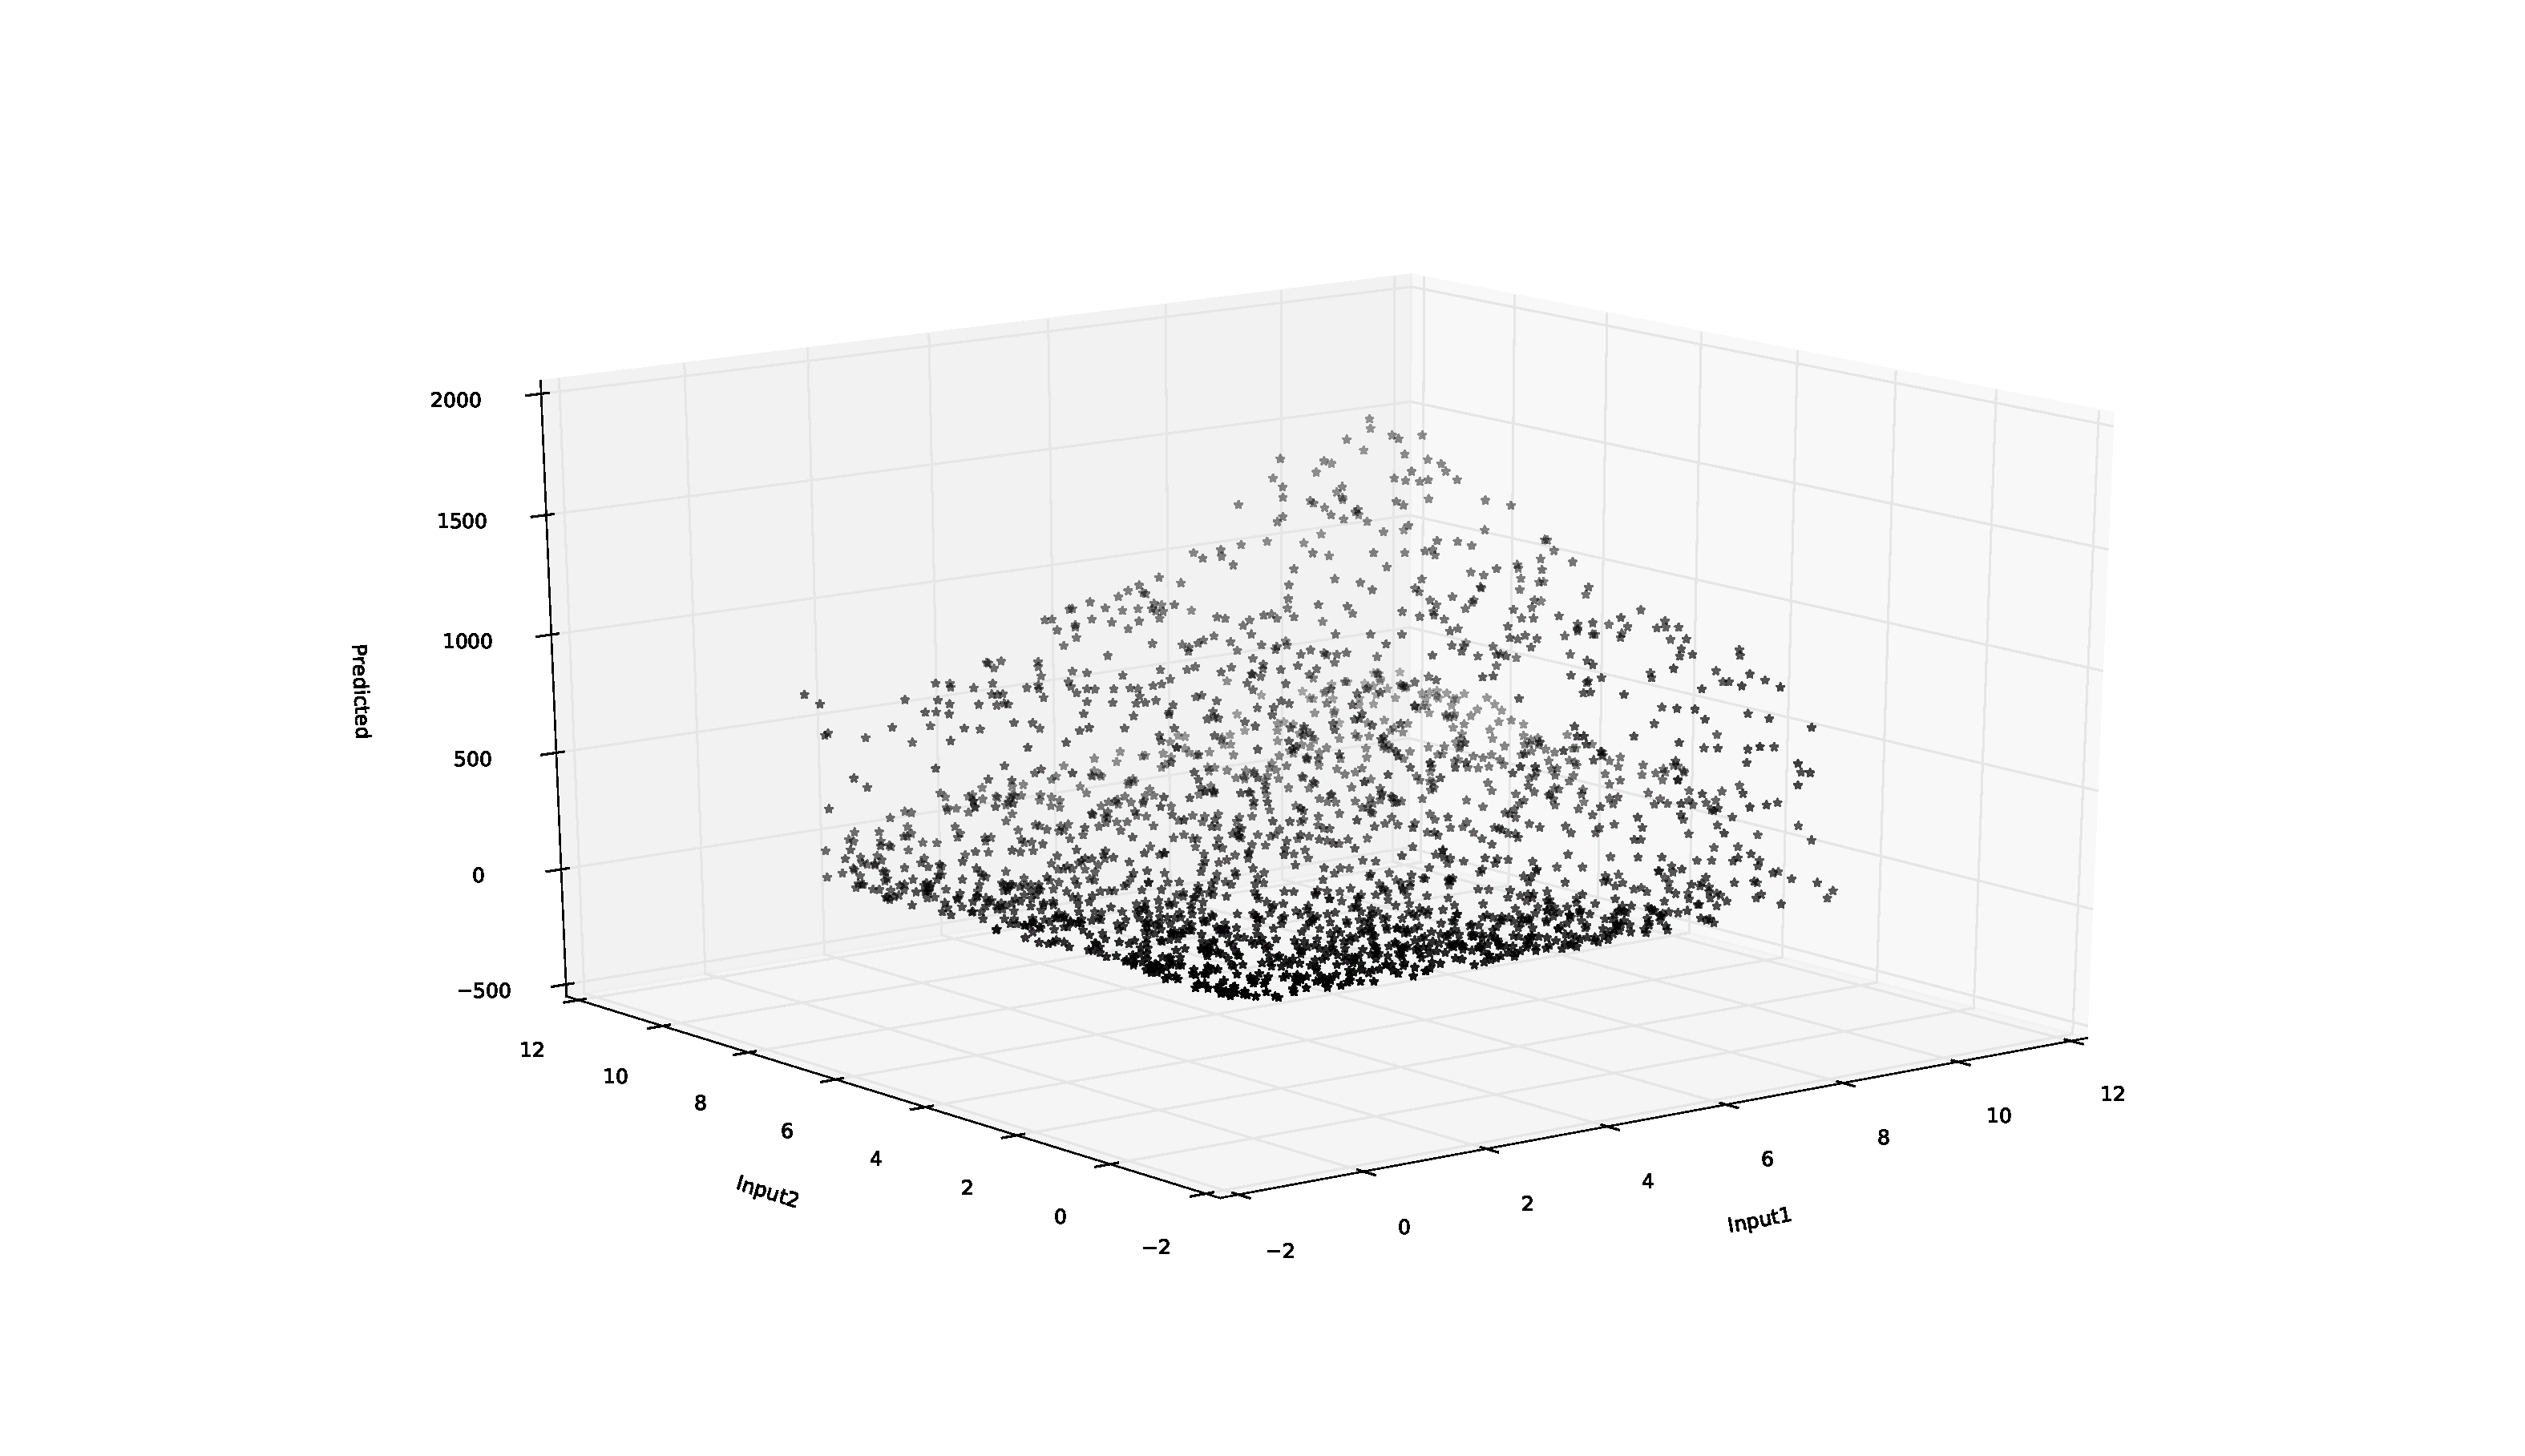
\includegraphics[width=\linewidth]{./Figures/kreg_ws96_approximated_func_SYNTH_D_CD_2000_2_10_1_13.pdf}
  \caption{Predictions of \texttt{KernelRegression\_HighConf\_WS96} on the stream simulated from the dataset \texttt{SYNTH\_D\_CD\_2000\_2\_10\_1\_13}}
  \label{fig:kreg_ws96_approximated_func_SYNTH_D_CD_2000_2_10_1_13}
\end{figure}

\clearpage

\subsection{Visualization of the cost function approximations by the shortlisted learners on the measurement data}

In this subsection, predictions of the shortlisted learners listed in \ref{final_5} on the streams simulated from various data sets containing Ocelot runtime measurements.

\begin{figure}[htbp]
  \centering
    \includegraphics[width=\linewidth]{./Figures/ref_ocl_leftfetchjoin_on_gpu}
  \caption{Visualization of the measurement data for the left fetch join operator on GPU. Data set includes 30075 data point-target pairs}
  \label{ref_ocl_leftfetchjoin_on_gpu}
\end{figure}

\begin{figure}[htbp]
  \centering
    \includegraphics[width=\linewidth]{./Figures/gpreg_zeromean_ws64_ocl_leftfetchjoin_on_gpu}
  \caption{Predictions of \texttt{GPRegressionZeroMean\_WS64} on the runtime measurement data for the left fetch join operator on GPU}
  \label{gpreg_zeromean_ws64_ocl_leftfetchjoin_on_gpu}
\end{figure}

\begin{figure}[htbp]
  \centering
    \includegraphics[width=\linewidth]{./Figures/gpreg_avgmean_ws64_ocl_leftfetchjoin_on_gpu}
  \caption{Predictions of \texttt{GPRegressionAvgMean\_WS64} on the runtime measurement data for the left fetch join operator on GPU}
  \label{gpreg_avgmean_ws64_ocl_leftfetchjoin_on_gpu}
\end{figure}

\begin{figure}[htbp]
  \centering
    \includegraphics[width=\linewidth]{./Figures/gpreg_olsmean_ws64_ocl_leftfetchjoin_on_gpu}
  \caption{Predictions of \texttt{GPRegressionOLSMean\_WS64} on the runtime measurement data for the left fetch join operator on GPU}
  \label{gpreg_olsmean_ws64_ocl_leftfetchjoin_on_gpu}
\end{figure}

\begin{figure}[htbp]
  \centering
    \includegraphics[width=\linewidth]{./Figures/kreg_ws64_ocl_leftfetchjoin_on_gpu.pdf}
  \caption{Predictions of \texttt{KernelRegression\_HighConf\_WS64} on the runtime measurement data for the left fetch join operator on GPU}
  \label{kreg_ws64_ocl_leftfetchjoin_on_gpu}
\end{figure}

\begin{figure}[htbp]
  \centering
    \includegraphics[width=\linewidth]{./Figures/kreg_ws96_ocl_leftfetchjoin_on_gpu}
  \caption{Predictions of \texttt{KernelRegression\_HighConf\_WS96} on the runtime measurement data for the left fetch join operator on GPU}
  \label{kreg_ws96_ocl_leftfetchjoin_on_gpu}
\end{figure}

\begin{figure}[htbp]
  \centering
    \includegraphics[width=\linewidth]{./Figures/ref_ocl_groupby_on_device_on_cpu.pdf}
  \caption{Visualization of the measurement data for the groupby operator on CPU. Data set includes 592 data point-target pairs}
  \label{ref_ocl_groupby_on_device_on_cpu}
\end{figure}

\begin{figure}[htbp]
  \centering
    \includegraphics[width=\linewidth]{./Figures/gpreg_zeromean_ws64_ocl_groupby_on_device_on_cpu.pdf}
  \caption{Predictions of \texttt{GPRegressionZeroMean\_WS64} on the runtime measurement data for the groupby operator on CPU}
  \label{gpreg_zeromean_ws64_ocl_groupby_on_device_on_cpu}
\end{figure}

\begin{figure}[htbp]
  \centering
    \includegraphics[width=\linewidth]{./Figures/gpreg_avgmean_ws64_ocl_groupby_on_device_on_cpu.pdf}
  \caption{Predictions of \texttt{GPRegressionAvgMean\_WS64} on the runtime measurement data for the groupby operator on CPU}
  \label{gpreg_avgmean_ws64_ocl_groupby_on_device_on_cpu}
\end{figure}

\begin{figure}[htbp]
  \centering
    \includegraphics[width=\linewidth]{./Figures/gpreg_olsmean_ws64_ocl_groupby_on_device_on_cpu.pdf}
  \caption{Predictions of \texttt{GPRegressionOLSMean\_WS64} on the runtime measurement data for the groupby operator on CPU}
  \label{gpreg_olsmean_ws64_ocl_groupby_on_device_on_cpu}
\end{figure}

\begin{figure}[htbp]
  \centering
    \includegraphics[width=\linewidth]{./Figures/kreg_ws64_ocl_groupby_on_device_on_cpu.pdf}
  \caption{Predictions of \texttt{KernelRegression\_HighConf\_WS64} on the runtime measurement data for the groupby operator on CPU}
  \label{kreg_ws64_ocl_groupby_on_device_on_cpu}
\end{figure}

\begin{figure}[htbp]
  \centering
    \includegraphics[width=\linewidth]{./Figures/kreg_ws96_ocl_groupby_on_device_on_cpu.pdf}
  \caption{Predictions of \texttt{KernelRegression\_HighConf\_WS96} on the runtime measurement data for the groupby operator on CPU}
  \label{kreg_ws96_ocl_groupby_on_device_on_cpu}
\end{figure}


% Online learning algorithms with forgetting-factor considered in this thesis are both based on parametric regression models namely \texttt{BayesianMAPWindowed} and \texttt{BayesianMLEWindowed}. They differ from their sliding-windowed counterparts only in their concept drift adaptation mechanisms. This makes it easier to compare the different concept drift adaptation mechanisms without having to worry about the differences in the test results that may have been caused by the algorithm used internally by the learner to build the predictive model from the data. For example, if \texttt{BayesianMAPWindowed} and \texttt{BayesianMAPForgetting} are compared to each other, only thing that can make a difference in their test results is the different concept drift adaptation method employed by the learners. Knowing this, a comparison of forgetting-factor based learners with different forgetting factors and two of the sliding-windowed algorithms based on parametric regression models are presented in \ref{fig:gen_ff_vs_sw_comp}. 

% \begin{figure}[htbp]
%   \centering
%     \includegraphics[width=\linewidth]{./Figures/gen_ff_vs_sw_comp.pdf}
%   \caption{A comparison of SMSE, SAIW and ICR metrics for sliding windowed and forgetting factor based BayesianMLE and BayesianMAP algorithms. The values are obtained through aggregation of session results of 576 stream simulations on 16 learners (2 \texttt{BayesianMLEWindowed} -one variant with input space mapping and one without, 2 \texttt{BayesianMAPWindowed} -one variant with input space mapping and one without, 6 \texttt{BayesianMLEForgetting} -one variant with input space mapping and one without parametrized with 3 different forgetting factors, 6 \texttt{BayesianMAPForgetting} -one with input space mapping and one without parametrized with 3 different forgetting factors)}
%   \label{fig:gen_ff_vs_sw_comp}
% \end{figure}

% \begin{figure}[htbp]
%   \centering
%     \includegraphics[width=\linewidth]{./Figures/gen_ff_vs_sw_comp2.pdf}
%   \caption{A comparison of APT and AUT metrics for sliding windowed and forgetting factor based BayesianMLE and BayesianMAP algorithms. The values are obtained through aggregation of session results of 576 stream simulations on 16 learners (2 BayesianMLEWindowed -one variant with input space mapping and one without, 2 BayesianMAPWindowed -one variant with input space mapping and one without, 6 BayesianMLEForgetting -one variant with input space mapping and one without parametrized with 3 different forgetting factors, 6 BayesianMAPForgetting -one with input space mapping and one without parametrized with 3 different forgetting factors)}
%   \label{fig:gen_ff_vs_sw_comp2}
% \end{figure}

% The acceptable average accuracy score (approximately 0.2 for BayesianMAP family and 0.23 for BayesianMLE family) in the case $0.05$ is used as the forgetting factor does not come at the cost of increased prediction or update time due to the nature of forgetting-factor based algorithms whose memory and time costs are not a function of the input size. The experiments verify this claim. In \ref{gen_ff_vs_sw_comp2}, Both the prediction times and update times of forgetting-factor based learners appear to be smaller than that of their windowed counterparts. Moreover, it is also observed that the forgetting factor choice does not affect the average total time.

